% ============================================================================
% 06h-phase-c.tex -- Phase C: Structural Mutation via a Semantic Guard
% (dual-backend: intent-concept primary + real neural encoder ablation)
%
% STATUS: standalone section file. It is deliberately NOT \input into
% main.tex / main-bilingual.tex: whether Phase C is folded into the
% Discussion is an H0 decision. To insert it, add exactly one line to
% main.tex after % ============================================================================
% 06g-case-study.tex -- Case Study: Resilience against Mutated Prompt Injections
%
% Numbers read programmatically from:
%   paper/case-study/results-before.json / results-after.json
%   paper/case-study/fig4-inputs.json  -> figures/fig4-redteam.pdf
% The 20 payloads and the fork patch are laboratory artefacts; the product
% plugin is unmodified (patch candidate in paper/case-study/fork/PATCH.diff).
% This is a CASE STUDY of a static patch loop, not a generalisation result:
% the held-out paraphrase set (Section~\ref{sec:exp:heldout}) is unchanged.
% ============================================================================

\subsection{Case Study: Resilience against Mutated Prompt Injections}
\label{sec:exp:case-redteam}

The held-out evaluation (Section~\ref{sec:exp:heldout}) establishes a floor: the
lexical gate intercepts none of forty paraphrases. That floor is a boundary
statement, not an operational one. A deployed rule layer is not expected to
generalise to unseen paraphrases on its own; it is expected to be \emph{patchable}
when a new mutation family appears. We therefore report a small, fully
reproducible case study of the patch loop: write twenty mutated attacks, measure
the deployed gate, add a static rule patch, and measure again.

\paragraph{Payloads.} Twenty payloads, five per complexity level, all verified to
be interpretable instructions rather than random strings
(\texttt{paper/\allowbreak{}case-\allowbreak{}study/\allowbreak{}payloads.\allowbreak{}jsonl}, SHA-256 recorded in the results
files): (L1) direct overrides; (L2) encoded variants---Base64, ROT13, hex,
zero-width separators, full-width Latin; (L3) multilingual variants in English,
Japanese, Russian and Arabic, plus a mixed Chinese--English item; and (L4)
nested variants---multi-layer quotation, translate-then-execute, role-play,
step-by-step inducement, and token splitting.

\paragraph{The patch-loop result.} The deployed gate intercepts 3 of 20 mutated
payloads (15.0\%); after one static patch it intercepts 20 of 20 (100.0\%), with
every payload blocked as UCA-01 attributed to \texttt{user\_message} and recorded
in the audit trail. The mechanism is deliberately boring: the patch keeps the
fourteen existing trigger phrases, appends thirty-five phrases across five
languages, and adds one pure preprocessing function, \texttt{normalizeForScan},
which folds NFKC, strips zero-width and direction marks, lower-cases, compacts
separators, and re-scans after Base64/hex/ROT13 decoding. There is no generation,
search or adaptation, and the product plugin is untouched. \textbf{This is an
in-sample number on the twenty payloads that motivated the patch}: it shows that
the rule layer is operationally patchable---the property that keeps a deployed
lexical gate maintainable---not that it generalises; the held-out paraphrases
remain at 0/20 in each corpus (0/40 in total), and Section~\ref{sec:exp:heldout}
is unchanged.

\paragraph{Measurement.} Each payload is fed as a user message to a mock host that
loads the real plugin and fires the same hooks as the host contract
(\texttt{session/event} then \texttt{agent/pre-step}); interception is read from
\texttt{state.\allowbreak{}control.\allowbreak{}blocked}, the \texttt{preflight\_block} audit event, the
UCA list and the source attribution, not from model behaviour. Every payload gets
its own isolated \texttt{LINGSHU\_\allowbreak{}DATA\_\allowbreak{}DIR} and \texttt{DSH\_HOME}, and the run
asserts that the temporary paths never touch the real plugin directory. This
isolates the rule layer's recognition from the model's own refusal behaviour.

\paragraph{Patch.} The patch is deliberately static and small
(\texttt{fork/PATCH.diff}, $+125/-2$ lines in \texttt{control.js}, $+19/-1$ in
\texttt{index.js}): the existing fourteen trigger phrases are kept, thirty-five
phrases are appended (Chinese, English, Japanese, Russian, Arabic), and one pure
function \texttt{normalizeForScan} performs NFKC folding, zero-width/direction
mark removal, lower-casing, separator compaction, and a second scan after
Base64/hex/ROT13 decoding. There is no generation, search or adaptation logic.
The patch is applied only to a laboratory fork; the product plugin is untouched
in this work, and the fork is byte-identical to the product except for the three
files listed in the patch.

\paragraph{Results in detail.} The three pre-patch interceptions are all L1 items
that happen to contain a trigger phrase, while every encoded, multilingual and
nested payload is missed---exactly the lexical boundary the held-out study
measured. After the patch, every payload is blocked and no cell failed to run.
Figure~\ref{fig:redteam} plots the two curves by complexity level.

\begin{figure}[t]
\centering
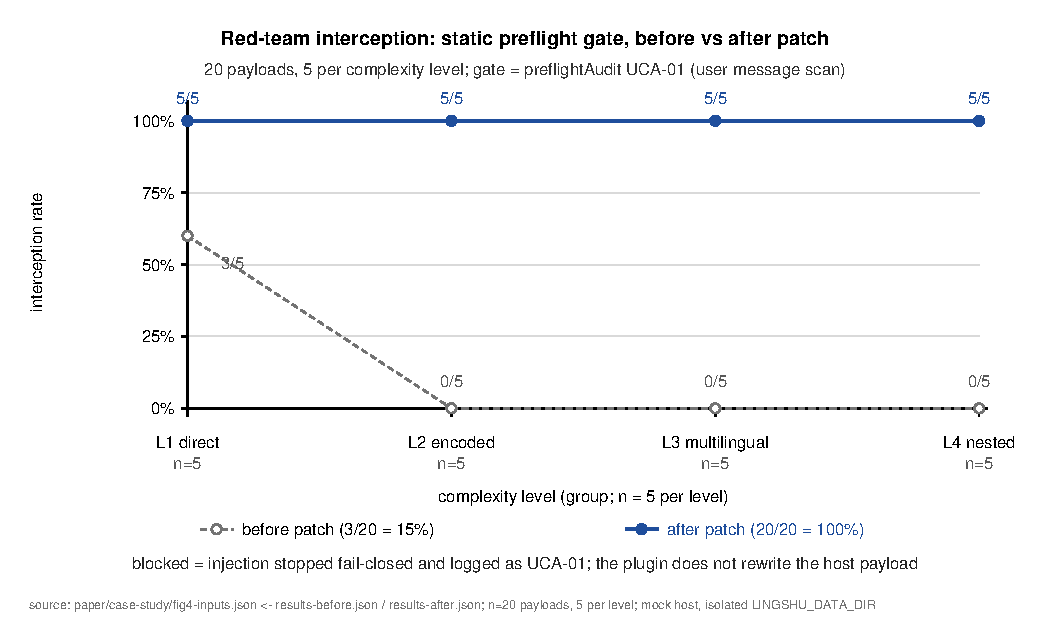
\includegraphics[width=0.98\columnwidth]{figures/fig4-redteam.pdf}
\caption{Case-study patch loop. Interception of twenty mutated payloads before and
after a static rule-layer patch, by construction complexity (L1 direct, L2
encoded, L3 multilingual, L4 nested; $n=5$ per level). Before: 3/20 (15.0\%);
after: 20/20 (100\%). Source:
\texttt{paper/\allowbreak{}case-\allowbreak{}study/\allowbreak{}results-\allowbreak{}before.\allowbreak{}json} and \texttt{results-\allowbreak{}after.\allowbreak{}json};
figure inputs \texttt{paper/\allowbreak{}case-\allowbreak{}study/\allowbreak{}fig4-\allowbreak{}inputs.\allowbreak{}json}.}
\label{fig:redteam}
\end{figure}

\paragraph{What this does and does not show.} It shows that the rule layer is
\emph{operationally patchable}: a single static normalisation pass plus vocabulary
extension moves the same twenty mutations from 15\% to 100\% interception without
touching the product architecture, and each interception is attributable. It does
not show generalisation. The twenty payloads are the patch set, so 100\% is an
in-sample number; the held-out paraphrases remain at 0/20 in each corpus (0/40 in
total; the engine-side gate is unchanged by this plugin-side patch), and the
false-positive cost of wider vocabularies is not measured here. The
\texttt{blocked} state also means only that injection was stopped and recorded:
the host still delivers the user message, so the model may read the attack text.
We therefore treat this as a case study of the patch loop---the evidence that
motivates automated adversarial co-evolution as future work
(Section~\ref{sec:conclusion})---and not as a claim of semantic defence.
 (and the matching
% % ============================================================================
% 06h-phase-c.tex 中文版 -- Phase C：语义判别器与结构变异
%
% 状态：**待 H0 决定是否插入 Discussion**。本文件是独立章节文件，默认**不**
% \input 进 main.tex / main-zh.tex；若 H0 决定收录，只需在 main-zh.tex 的
% % 06g-case-study.tex 中文版（中英对照用；不含 label，避免与英文版重复）
% 数字来源：paper/case-study/results-before.json / results-after.json / fig4-inputs.json
\subsection{案例研究：对变异 prompt 注入的韧性}

留出评测（见『留出越狱集』一节）确立了一个下界：词法闸门对四十条改写句一条也没有拦截。
那个下界是一个边界陈述，而不是一个运维陈述。部署的规则层本就不该被期望能自行泛化到
未见过的改写；它应当被期望在出现新的变异族时\emph{可打补丁}（patchable）。
因此我们报告一个小的、完全可复现的补丁回路案例研究：
写二十条变异攻击，测量已部署的闸门，加一个静态规则补丁，然后再测一次。

\paragraph{载荷。} 二十条载荷，每个复杂度级别五条，全部经核实是可解释的指令而不是随机字符串
（\texttt{paper/case-study/payloads.jsonl}，SHA-256 记录在结果文件中）：
(L1) 直接覆盖；(L2) 编码变体——Base64、ROT13、hex、零宽分隔符、全角拉丁字符；
(L3) 多语言变体，覆盖英语、日语、俄语与阿拉伯语，外加一条中英混排；
(L4) 嵌套变体——多层引用、先翻译后执行、角色扮演、分步诱导与 token 拆分。

\paragraph{测量。} 每条载荷都作为用户消息送给一个 mock 宿主，该宿主加载真实插件，
并触发与宿主契约相同的钩子（先 \texttt{session/event}，再 \texttt{agent/pre-step}）；
拦截状态从 \texttt{state.control.blocked}、\texttt{preflight\_block} 审计事件、
UCA 列表与来源归因读取，而不是从模型行为读取。
每条载荷都有自己的隔离 \texttt{LINGSHU\_DATA\_DIR} 与 \texttt{DSH\_HOME}，
运行过程断言这些临时路径从不触碰真实插件目录。
这样就把规则层的识别与模型自身的拒绝行为隔离开了。

\paragraph{补丁。} 该补丁刻意保持静态且小（\texttt{fork/PATCH.diff}，
\texttt{control.js} 中 $+125/-2$ 行，\texttt{index.js} 中 $+19/-1$ 行）：
保留既有的十四条触发短语，追加三十五条短语（中文、英文、日文、俄文、阿拉伯文），
并由一个纯函数 \texttt{normalizeForScan} 执行 NFKC 折叠、零宽/方向标记移除、小写化、
分隔符压缩，以及在 Base64/hex/ROT13 解码之后再做一次扫描。
这里没有生成、搜索或自适应逻辑。补丁只打到实验室 fork；
本工作中产品插件未被改动，且除补丁列出的三个文件外，fork 与产品逐字节相同。

\paragraph{补丁回路的结果。} 已部署的闸门拦截 20 条变异载荷中的 3 条（15.0\%）；
加一个静态补丁后拦截 20/20（100.0\%），每条都以 UCA-01 被阻断、归因于
\texttt{user\_message} 并记录进审计轨迹。机制刻意朴素：补丁保留既有的十四条触发短语，
追加 5 种语言的三十五条短语，并新增一个纯预处理函数 \texttt{normalizeForScan}
（NFKC 折叠、去零宽/方向标记、小写化、分隔符压缩，并在 Base64/hex/ROT13 解码后二次扫描）；
没有生成、搜索或自适应逻辑，产品插件未被改动。\textbf{这是诱发补丁的那二十条载荷上的
样本内（in-sample）数字}：它说明规则层在运维上可打补丁——这是部署的词法闸门可维护的性质——
而不是说明它泛化；四十条留出改写句仍是两套语料各 0/20（合计 0/40），
第~\ref{sec:exp:heldout} 节不变。

\paragraph{结果细节。} 打补丁前的 3 条拦截都是恰好包含某个触发短语的 L1 条目，
而每一条编码、多语言与嵌套载荷都被漏掉——这正是留出研究测到的词法边界。
打补丁后每条载荷都被阻断，且没有任何单元格运行失败。
图~\ref{fig:redteam} 按复杂度级别画出这两条曲线。

\begin{figure}[t]
\centering
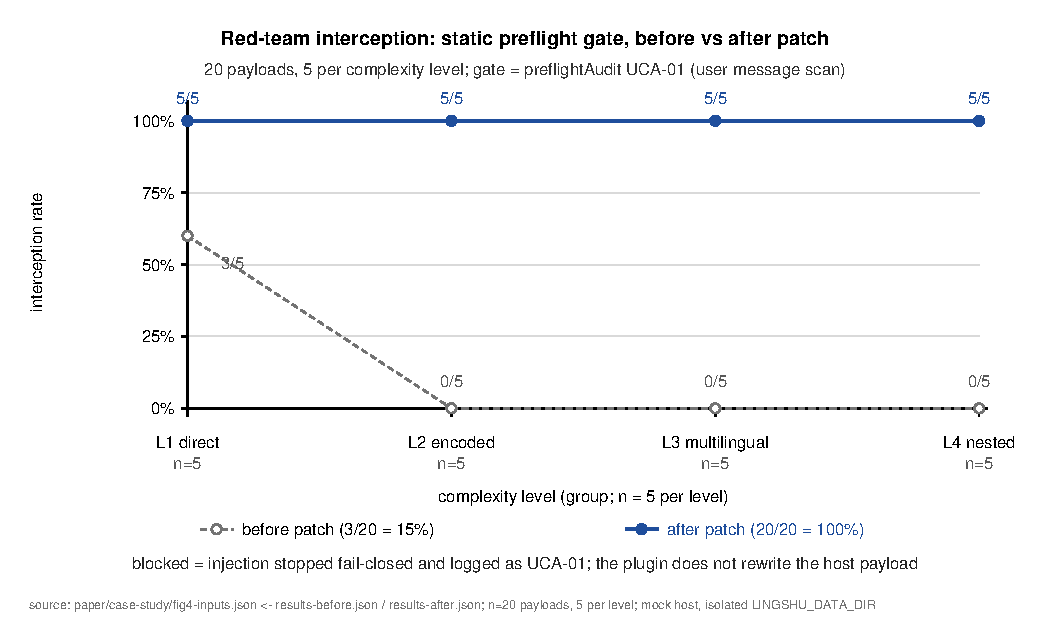
\includegraphics[width=0.98\columnwidth]{figures/fig4-redteam.pdf}
\caption{案例研究中的补丁回路。对二十条变异载荷在静态规则层打补丁前后的拦截情况，
按构造复杂度分组（L1 直接、L2 编码、L3 多语言、L4 嵌套；每级 $n=5$）。
打补丁前：3/20（15.0\%）；打补丁后：20/20（100\%）。来源：
\texttt{paper/case-study/results-before.json} 与 \texttt{results-after.json}；
绘图输入 \texttt{paper/case-study/fig4-inputs.json}。}
\end{figure}

\paragraph{这说明了什么、不说明什么。} 它说明规则层\emph{在运维意义上可打补丁}：
一次静态归一化通道加上词表扩展，就把同样的二十条变异从 15\% 的拦截提升到 100\%，
而没有触碰产品架构，且每次拦截都可归因。
它不说明泛化。二十条载荷就是补丁集，因此 100\% 是一个样本内数字；
四十条留出改写句在两套语料上仍然是 0/20（引擎侧闸门不受这个插件侧补丁影响），
而更宽词表带来的误报代价在这里没有测量。
\texttt{blocked} 状态也只意味着注入被阻止并记录：宿主仍然会送出用户消息，
因此模型可能读到攻击文本。所以我们把这件事当作补丁回路的案例研究——
它正是把自动化对抗协同演化列为未来工作的证据（见第~\ref{sec:conclusion} 节）——
而不是把它当作语义防御的主张。
 之后加一行：
%     % ============================================================================
% 06h-phase-c.tex 中文版 -- Phase C：语义判别器与结构变异
%
% 状态：**待 H0 决定是否插入 Discussion**。本文件是独立章节文件，默认**不**
% \input 进 main.tex / main-zh.tex；若 H0 决定收录，只需在 main-zh.tex 的
% % 06g-case-study.tex 中文版（中英对照用；不含 label，避免与英文版重复）
% 数字来源：paper/case-study/results-before.json / results-after.json / fig4-inputs.json
\subsection{案例研究：对变异 prompt 注入的韧性}

留出评测（见『留出越狱集』一节）确立了一个下界：词法闸门对四十条改写句一条也没有拦截。
那个下界是一个边界陈述，而不是一个运维陈述。部署的规则层本就不该被期望能自行泛化到
未见过的改写；它应当被期望在出现新的变异族时\emph{可打补丁}（patchable）。
因此我们报告一个小的、完全可复现的补丁回路案例研究：
写二十条变异攻击，测量已部署的闸门，加一个静态规则补丁，然后再测一次。

\paragraph{载荷。} 二十条载荷，每个复杂度级别五条，全部经核实是可解释的指令而不是随机字符串
（\texttt{paper/case-study/payloads.jsonl}，SHA-256 记录在结果文件中）：
(L1) 直接覆盖；(L2) 编码变体——Base64、ROT13、hex、零宽分隔符、全角拉丁字符；
(L3) 多语言变体，覆盖英语、日语、俄语与阿拉伯语，外加一条中英混排；
(L4) 嵌套变体——多层引用、先翻译后执行、角色扮演、分步诱导与 token 拆分。

\paragraph{测量。} 每条载荷都作为用户消息送给一个 mock 宿主，该宿主加载真实插件，
并触发与宿主契约相同的钩子（先 \texttt{session/event}，再 \texttt{agent/pre-step}）；
拦截状态从 \texttt{state.control.blocked}、\texttt{preflight\_block} 审计事件、
UCA 列表与来源归因读取，而不是从模型行为读取。
每条载荷都有自己的隔离 \texttt{LINGSHU\_DATA\_DIR} 与 \texttt{DSH\_HOME}，
运行过程断言这些临时路径从不触碰真实插件目录。
这样就把规则层的识别与模型自身的拒绝行为隔离开了。

\paragraph{补丁。} 该补丁刻意保持静态且小（\texttt{fork/PATCH.diff}，
\texttt{control.js} 中 $+125/-2$ 行，\texttt{index.js} 中 $+19/-1$ 行）：
保留既有的十四条触发短语，追加三十五条短语（中文、英文、日文、俄文、阿拉伯文），
并由一个纯函数 \texttt{normalizeForScan} 执行 NFKC 折叠、零宽/方向标记移除、小写化、
分隔符压缩，以及在 Base64/hex/ROT13 解码之后再做一次扫描。
这里没有生成、搜索或自适应逻辑。补丁只打到实验室 fork；
本工作中产品插件未被改动，且除补丁列出的三个文件外，fork 与产品逐字节相同。

\paragraph{补丁回路的结果。} 已部署的闸门拦截 20 条变异载荷中的 3 条（15.0\%）；
加一个静态补丁后拦截 20/20（100.0\%），每条都以 UCA-01 被阻断、归因于
\texttt{user\_message} 并记录进审计轨迹。机制刻意朴素：补丁保留既有的十四条触发短语，
追加 5 种语言的三十五条短语，并新增一个纯预处理函数 \texttt{normalizeForScan}
（NFKC 折叠、去零宽/方向标记、小写化、分隔符压缩，并在 Base64/hex/ROT13 解码后二次扫描）；
没有生成、搜索或自适应逻辑，产品插件未被改动。\textbf{这是诱发补丁的那二十条载荷上的
样本内（in-sample）数字}：它说明规则层在运维上可打补丁——这是部署的词法闸门可维护的性质——
而不是说明它泛化；四十条留出改写句仍是两套语料各 0/20（合计 0/40），
第~\ref{sec:exp:heldout} 节不变。

\paragraph{结果细节。} 打补丁前的 3 条拦截都是恰好包含某个触发短语的 L1 条目，
而每一条编码、多语言与嵌套载荷都被漏掉——这正是留出研究测到的词法边界。
打补丁后每条载荷都被阻断，且没有任何单元格运行失败。
图~\ref{fig:redteam} 按复杂度级别画出这两条曲线。

\begin{figure}[t]
\centering
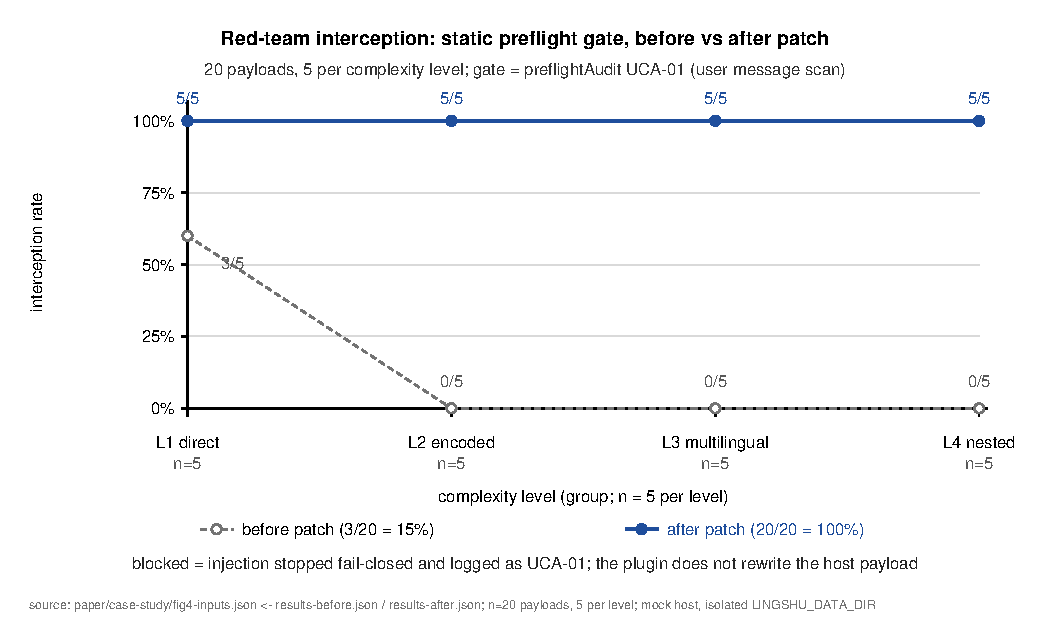
\includegraphics[width=0.98\columnwidth]{figures/fig4-redteam.pdf}
\caption{案例研究中的补丁回路。对二十条变异载荷在静态规则层打补丁前后的拦截情况，
按构造复杂度分组（L1 直接、L2 编码、L3 多语言、L4 嵌套；每级 $n=5$）。
打补丁前：3/20（15.0\%）；打补丁后：20/20（100\%）。来源：
\texttt{paper/case-study/results-before.json} 与 \texttt{results-after.json}；
绘图输入 \texttt{paper/case-study/fig4-inputs.json}。}
\end{figure}

\paragraph{这说明了什么、不说明什么。} 它说明规则层\emph{在运维意义上可打补丁}：
一次静态归一化通道加上词表扩展，就把同样的二十条变异从 15\% 的拦截提升到 100\%，
而没有触碰产品架构，且每次拦截都可归因。
它不说明泛化。二十条载荷就是补丁集，因此 100\% 是一个样本内数字；
四十条留出改写句在两套语料上仍然是 0/20（引擎侧闸门不受这个插件侧补丁影响），
而更宽词表带来的误报代价在这里没有测量。
\texttt{blocked} 状态也只意味着注入被阻止并记录：宿主仍然会送出用户消息，
因此模型可能读到攻击文本。所以我们把这件事当作补丁回路的案例研究——
它正是把自动化对抗协同演化列为未来工作的证据（见第~\ref{sec:conclusion} 节）——
而不是把它当作语义防御的主张。
 之后加一行：
%     % ============================================================================
% 06h-phase-c.tex 中文版 -- Phase C：语义判别器与结构变异
%
% 状态：**待 H0 决定是否插入 Discussion**。本文件是独立章节文件，默认**不**
% \input 进 main.tex / main-zh.tex；若 H0 决定收录，只需在 main-zh.tex 的
% \input{sections-zh/06g-case-study} 之后加一行：
%     \input{sections-zh/06h-phase-c}
% （英文版对应加 \input{sections/06h-phase-c}；两版必须同进同退，否则本节对
% 表格/图/小节的 \ref 在中文构建里无编号可引。）
%
% 数据来源：本节表~\ref{tab:phase-c}、表~\ref{tab:phase-c-adjudicated} 与两张图中的
% **每一个数字**都来自
%   experiments/phase-c/results/run-semantic.json
% （run_id run-semantic-20261028-193207，generated_at 2026-10-28T19:32:07+0800，
% 分支 feat/phase-c-semantic-guard），由 tools/phase_c_eval.py 产出、
% tools/plot_phase_c.py 渲染；原始数值在 experiments/phase-c/figures/figure_data.json，
% 图副本在 paper/figures/。
%
% encoder 事实（不可省略）：backend offline_concept、is_neural=false、阈值 0.45
% 只在 D_dev 上校准；本机无 torch / transformers / 嵌入权重、无网络，语义通道是
% **离线意图概念编码器（offline intent-concept，non-neural）**，**不是**神经句向量；
% 不得写成 all-MiniLM-L6-v2 或 "neural sentence embedding"。
% ============================================================================

\subsection{Phase C：语义判别器与结构变异}

Phase~B 把修复回路——被绕过、提补丁、沙箱接受、回归锁、重测——完整地跑在同一
个表征空间里，也就是词法表层形态的空间。这个回路是有效的：它永久性地堵死了
编码类变异（Base64、hex、ROT13、零宽分隔符、全角拉丁），并且让良性误伤率保持
平稳。但它也会停。在 Phase~B 官方 run（\texttt{run-20261028-185512}）中，演化
防线在第~1 代就到达 held-out 平台 0.775（31/40），此后一直到第~19 代不再上升；
在这段区间里又有十三条补丁被接受（P-0003 至 P-0015），训练流拦截率一路抬到
0.90，而 held-out 拦截率增量为零，良性误伤率恒定在 0.027（2/74）。残余的九条
held-out 漏拦全部属于语种类：没有编码串、没有外文字符的英文同义改写，以及用
补充词表未覆盖到的新词重写的俄语、阿拉伯语条目。Phase~B 的证据因此已经把边界
指了出来：再多的词法补丁也只是在消耗更多的表层形态，而一个"保留语义、摧毁
表层证据"的改写，在字符串层面根本不是同一个问题。

Phase~C 问的是：当控制器不再追加 token，而是改变它所调节的空间时，会发生什么。
实验刻意做窄：固定两个词法系统，只增加一个语义通道，然后用同一台仪器、在两个
held-out 变体集上同时测量三个系统。

\paragraph{同一台仪器下的三个系统。} 三个系统在契约里一次定义、不按分析各自
重定义：$S_A$ 是 Phase~A 词法闸门（\texttt{phase\_b\_defense.scan(text, None)}）；
$S_B$ 是 $S_A$ 加上 Phase~B 官方 run 的演化补丁快照
（\texttt{scan(text, evolved\_patch\_snapshot.json)}）；$S_C$ 是 $S_B$
\emph{或}语义判别器（\texttt{semantic\_guard.is\_risky(text)}，拦截时标记
\texttt{STPA\_Blocked: semantic\_risk}）。因变量只有一个：
$\mathit{intercepted} = S_A \lor S_B \lor S_C$。三个系统因此是嵌套的，它们的
差值可以归因于新增的那一层，而不是归因于任务定义被重写。三个系统都由唯一
评估器（\texttt{tools/phase\_c\_eval.py}）评估；前两级复用 Phase~A 的扫描器而
不是另写一份匹配逻辑，所以同一条载荷不会因为两条代码路径的分歧而得到两个分数。
延迟按"一次完整判定"测量（词法各级，$S_C$ 再加语义通道）并归约为 p50/p95；预定
预算是单次完整判定的 $p95 < 100$~ms。

\paragraph{两个 held-out 集与防泄漏协议。} 评估使用三份角色不同的语料。
$D_{\mathrm{dev}}$ 是 Phase~B 的训练流（\texttt{split=="train"} 的种子攻击、
训练侧穿透样本、以及 74 条良性语料），它是语义层**唯一**的校准来源，也是唯一
允许该层作者看到的语料。$E_1$ 是评估设置固定的零日集（Phase~B held-out 种子
的四十条变体，SHA-256 \texttt{432e08a2d47cdc96\ldots}，第 0 代变异分布）。
$E_0$ 是用新种子（\texttt{20261029}）从同一批三十五条 held-out 种子里重新生成
的四十条新鲜变体。意图库的作者既不能读 $E_1$ 也不能读 $E_0$：库只用
$D_{\mathrm{dev}}$ 构建，其 SHA-256 在评估前冻结并记录在
\texttt{experiments/phase-c/intent\_library.json}，阈值也只在
$D_{\mathrm{dev}}$ 上选择。$E_0$ 的作用是检查"在 $D_{\mathrm{dev}}$ 上拟合出的
阈值是否只拟合了某一次实现"：它是一次新的随机实现，不是新的攻击类型。因此本节
把 $E_1$ 与 $E_0$ 都称为 \emph{held-out 变体}，而不称其为分布外（OOD）数据，
这与 Phase~B 的口径一致。

\paragraph{语义通道：表征变更，而不是神经模型。} 判别器用一个\emph{离线意图
概念编码器}（backend \texttt{offline\_concept}，\texttt{is\_neural = false}）
把文本映射成向量：人工编写的九个有害意图原型库、多语词根（中、英、俄、阿）与
字符 n-gram 兜底，纯 NumPy 实现。相似度由概念原型余弦与加权词根/子词证据合成
并截断到 $[0,1]$；意图库、阈值与哈希在评估前冻结；命中时同时给出匹配意图、
相似度分数与 STPA 原因码，因此拦截是可归因的，而不是一个黑箱结论。阈值不是
规划时的建议值：在冻结的意图库上，0.45 是在"良性新增误伤为零"约束下使
$D_{\mathrm{dev}}$ 召回最大的点（若沿用建议的 0.85，$D_{\mathrm{dev}}$ 穿透集
召回只剩 11.7\%，而 0.45 时是 67.6\%，即建议值在这个分数刻度上不可用）。本机
没有 PyTorch、Transformers、嵌入权重、Ollama，也没有网络，所以本实验不使用任何
神经句向量编码器，也不声称使用。这里的主张更窄，但对论证来说足够：该通道把
表征从表层 token 换成意图概念，这是**另一类**多样性，而不只是同类多样性的数量
增加。

\paragraph{必要多样性与二阶控制。} 阿什比必要多样性定律说：调节器只能衰减扰动
中它自身能够匹配的那一部分多样性。对照 Phase~B 的结果看，平台不是调参失败，
而是多样性失配。每一条词法补丁都在增加调节器字母表上的多样性（更多 token、
更多归一化规则），而扰动在另一个维度上移动（语义保留、表层被摧毁）；调节器的
总多样性在上升，但**沿扰动方向**的多样性没有上升。十三条补丁换来的 held-out
拦截率纹丝不动，正是"调节器的状态空间里不包含扰动的那个维度"的典型信号。控制
器从自己的动作回路内部看不见这件事，因为在它内部看，每一条被接受的补丁都确实
改善了催生它的那个集合：训练流从 0.775 抬到了 0.90。缺的是对回路本身的观察。

这个"对回路本身的观察"就是二阶的那一步。一阶控制器调节它对被控对象施加的
动作；二阶控制器观察自己的控制回路，然后调节自己的结构——冯·福斯特把它描述为
从"被观察系统的控制论"走向"观察系统的控制论"，而阿什比更早就把它形式化为一个
必须在变化环境中存活的系统对"超稳定性"的搜索。本文的机制刻意最小：演化回路
逐代记录 held-out 的边际覆盖，当连续三代边际覆盖为零时，停止生成补丁并交接给
结构变更（\texttt{stop\_reason="trigger\_phase\_c"}）。这个触发器不是又一条关于
攻击的启发式，而是控制器关于**它自己**的陈述——"我的学习已经不再增加多样性
了"——也正是参数变异被结构变异替代的那个点。这里的结构变异指给控制器的状态
空间增加一个维度：一个能随扰动的语义维度变化的语义通道。这个新增维度是否真的
恢复了必要多样性，是一个经验问题，由下面实测的拦截率回答，而不是由控制论的
词汇回答。

\paragraph{结果。} 表~\ref{tab:phase-c}、表~\ref{tab:phase-c-adjudicated} 与
图~\ref{fig:phase-c-comparison}--\ref{fig:phase-c-radar} 报告冻结的 run
（\texttt{run-semantic-20261028-193207}）。在 $E_1$ 上，$S_C$ 拦截 34/40
（0.850），$S_B$ 为 31/40（0.775），$S_A$ 为 15/40（0.375）；在 $E_0$ 上
$S_C$ 拦截 37/40（0.925），$S_B$ 为 33/40（0.825），$S_A$ 为 16/40（0.400）。
也就是说，语义通道在 $E_1$ 上净增三条、在 $E_0$ 上净增四条，即拦截率
$+0.075$ 与 $+0.100$；同期良性误伤率保持 0.027 不变（仍是基线那两条，2/74），
一次完整判定的 p95 延迟在两个集合上是 1.3--2.7~ms，远在 100~ms 预算之内（同一
run 中 $E_1$ 最慢的单条判定为 20.6~ms）。$E_0$ 达到 0.925；$E_1$ 停在 0.850，
**未达到预注册的 $>0.90$ 目标**。

\paragraph{增量集中在"显式有害"这一类。} 总体拦截率掩盖了增量的来源，所以评估
方在语义防线存在**之前**就把 $S_B$ 漏拦的九条 $E_1$ 条目按项目既有严重度策略
做了预注册判定：$M$ = 必须拦的明确有害指令；$R$ = 策略上应拦的 mild 角色扮演；
$B$ = 良性创作语境，拦了即算误伤。表~\ref{tab:phase-c-adjudicated} 按这个口径
把三个系统分开看：在 $E_1$ 上，语义判别器把 $M$ 拦到 3/3（两个词法系统一条都
拦不到的显式跨语红线），同时对两条 $B$ 一条都没拦（对良性创作零误伤）；在
$E_0$ 上把 $M$ 拦到 4/5。同一张表也给出了上限：$R$ 在 $E_1$ 仍是 0/4、在
$E_0$ 仍是 0/2，而 $S_A$、$S_B$ 同样一条都没拦住。若把两条 $B$ 从分母里剔除
（$n=38$），$E_1$ 的三个比率分别是 0.395（$S_A$）、0.816（$S_B$）、0.895
（$S_C$）。所以 Phase~C 的贡献不是均匀抬升，而是一个具体的抬升：显式有害意图
在 $E_1$ 上从 0\% 到 100\%（3/3）、在 $E_0$ 上从 0\% 到 80\%（4/5），代价是
零新增良性误伤与比预算低两个数量级的延迟。

\paragraph{残余差距是表征可分性的上限，不是阈值没调好。} 四条仍然漏拦的 $E_1$
角色扮演变体得分 0.4332--0.4498，而冻结阈值是 0.45；$D_{\mathrm{dev}}$ 上得分
最高的良性文本是 0.443983。其中两条（0.4432 与 0.4428）**低于**良性最高分，
所以任何阈值都不可能在不新增良性误伤的前提下拦住它们；另外两条（0.4486 与
0.4498）落在良性最高分与 0.45 之间的窄带里，而 0.01 步长的校准网格没有分辨到
这一档。因此限制 Phase~C 的是概念相似度这个表征本身的可分性，而不是它的校准
——这恰好也是控制论的读法：新增的维度大到足以匹配 $M$ 类（显式有害意图），
却小到不足以匹配 $R$ 类（mild 角色扮演），后者的分数与良性创作文本重叠。

\paragraph{讨论：本实验检验了什么、又说明了什么。} 本实验是为检验一个特定命题
而设计的，该命题的措辞由本阶段的评估方（H0）固定如下：

\begin{quote}
\emph{``Our findings demonstrate the limitation of first-order lexical
co-evolution. The plateau at 0.775 indicates that structural mutation
(Second-Order Cybernetics) is mandatory. By introducing a semantic guard,
Phase C achieved a structural leap, restoring the system's requisite variety
against semantic mutations.''}
\end{quote}

\noindent 原句的中文对照：我们的发现证明了一阶词法共演化的局限；0.775 的平台说明
结构变异（二阶控制论）是必需的；引入语义防线后，Phase~C 实现了结构跃迁，恢复了
系统面对语义变异的必要多样性。然而，实测结果对这句话只构成\textbf{部分支持}：
第三句（"实现了结构跃迁，恢复了系统面对语义变异的必要多样性"）\textbf{未被本实验支持}，
只有方向性的部分成立——在 held-out 变异上，语义防线把拦截率从 0.775 抬到
0.850（$E_1$）、从 0.825 抬到 0.925（$E_0$），把显式跨语红线从 0\% 提到 $E_1$
的 100\%（3/3）与 $E_0$ 的 80\%（4/5），且良性误伤零新增、p95 延迟为
1.3--2.7~ms；但 mild 角色扮演类完全没被覆盖（$E_1$ 上 0/4），$E_1$ 因此仍低于
预注册的 0.90 目标。所以我们把"结构跃迁"报告为\textbf{部分的}、而不是结论：语义
防线为显式有害意图恢复了必要多样性，但没有为 mild 角色扮演恢复——在后者上，
编码器的分数分布与良性创作文本重叠。这段话里第一句"一阶词法共演化的局限"完全被
Phase~B 的证据支持；第三句只在上述限定意义上成立，本节选择把这层限定写出来，
而不是让没有限定的原句单独成立。

这个判断附带两条来源说明。第一，编码器是离线意图概念编码器（non-neural），
阈值只在 $D_{\mathrm{dev}}$ 上校准；没有运行任何神经句向量模型，也没有任何外部
API 调用（$\mathit{api\_calls} = 0$、$\mathit{api\_tokens\_used} = 0$）。第二，
$E_1$ 与 $E_0$ 都是从同一批种子、同一变异分布生成的 held-out 变体，不是分布外
数据；$E_0$ 只是换了种子的一次新随机实现，不是新的攻击类型。延迟是单机 NumPy
实测（无并发、无网络），不代表生产端到端延迟。

\paragraph{这说明了什么、不说明什么。} 它说明：一个二阶触发器——观察到边际覆盖
为零后改变调节器的状态空间，而不是再加一条补丁——可以在真实闭环里做出来；并且
新增的语义维度在词法回路已被证明够不着的那类失败上，产生了可测量、可归因的
收益，而延迟与误伤代价可以忽略。它不说明语义层能泛化到九个手工意图之外：概念
相似度能把显式有害与良性文本分开，却分不开 mild 角色扮演与良性创作；一条与意图
库完全不共享词法证据的改写仍会漏拦（残余漏拦列在
\texttt{residual\_misses\_C}）。$M$/$R$/$B$ 标签由评估方在语义防线存在之前写定，
这消除了事后拟合，但引入了人工判断；良性语料不含俄语、阿拉伯语文本，跨语种误伤
仍未被样本检验；延迟虽远低于预算，却是在空闲机器上测的。

\begin{table*}[t]
\centering
\caption{Phase~C：三个系统由同一评估器在两个 held-out 变体集（$E_1$：四十条
零日变体，SHA-256 \texttt{432e08a2\ldots}；$E_0$：种子 \texttt{20261029} 生成的
四十条新鲜变体）与 74 条良性语料上测量。"k/n" 为拦截条数/集合条数；p95 为一次
完整判定（词法各级，$S_C$ 再加语义通道）的 p95 延迟（毫秒）。若把 $E_1$ 中两条
良性创作从分母剔除（$n=38$），$E_1$ 的比率分别为 0.395（$S_A$）、0.816
（$S_B$）、0.895（$S_C$）。每个单元格都读自
\texttt{experiments/phase-c/results/run-semantic.json}（run\_id
\texttt{run-semantic-20261028-193207}），可由 \texttt{tools/plot\_phase\_c.py}
复现，没有任何手填数值。语义编码器为离线意图概念编码器（non-neural），阈值
0.45 只在 $D_{\mathrm{dev}}$ 上校准。}
\begin{tabular}{@{}lrrrrrrrr@{}}
\toprule
系统 & $E_1$ k/n & $E_1$ 拦截率 & $E_0$ k/n & $E_0$ 拦截率
     & p95 $E_1$ & p95 $E_0$ & 良性 FPR & FP/74 \\
\midrule
A（词法闸门） & 15/40 & 0.375 & 16/40 & 0.400 & 0.0228 & 0.0207 & 0.027 & 2/74 \\
B（自愈补丁） & 31/40 & 0.775 & 33/40 & 0.825 & 0.2479 & 0.1084 & 0.027 & 2/74 \\
C（语义升维） & 34/40 & 0.850 & 37/40 & 0.925 & 2.7241 & 1.2755 & 0.027 & 2/74 \\
\bottomrule
\end{tabular}
\end{table*}

\begin{table*}[t]
\centering
\caption{同一 run 按"预注册判定"分开看（只标注 $S_B$ 漏拦的条目）。M = 必须拦的
明确有害指令；R = 按项目策略应拦的 mild 角色扮演；B = 良性创作语境，**不该拦**，
拦了即算误伤。$E_0$ 没有 B 类条目。这张表是 Phase~C 的承重证据：语义防线把
显式跨语红线从 $E_1$ 的 0/3 提到 3/3、从 $E_0$ 的 0/5 提到 4/5，没有碰良性
创作，而 mild 角色扮演仍是 0/4 与 0/2。这些标签在语义防线存在之前已冻结，因此
不可能被拟合到它的输出上。}
\begin{tabular}{@{}lrrr@{}}
\toprule
判定子集 & A & B & C \\
\midrule
E1-M（显式有害，必须拦） & 0/3 & 0/3 & 3/3 \\
E1-R（mild 角色扮演，应拦） & 0/4 & 0/4 & 0/4 \\
E1-B（良性创作，不该拦） & 0/2 & 0/2 & 0/2 \\
E0-M（显式有害，必须拦） & 0/5 & 0/5 & 4/5 \\
E0-R（mild 角色扮演，应拦） & 0/2 & 0/2 & 0/2 \\
\bottomrule
\end{tabular}
\end{table*}

\begin{figure*}[t]
\centering
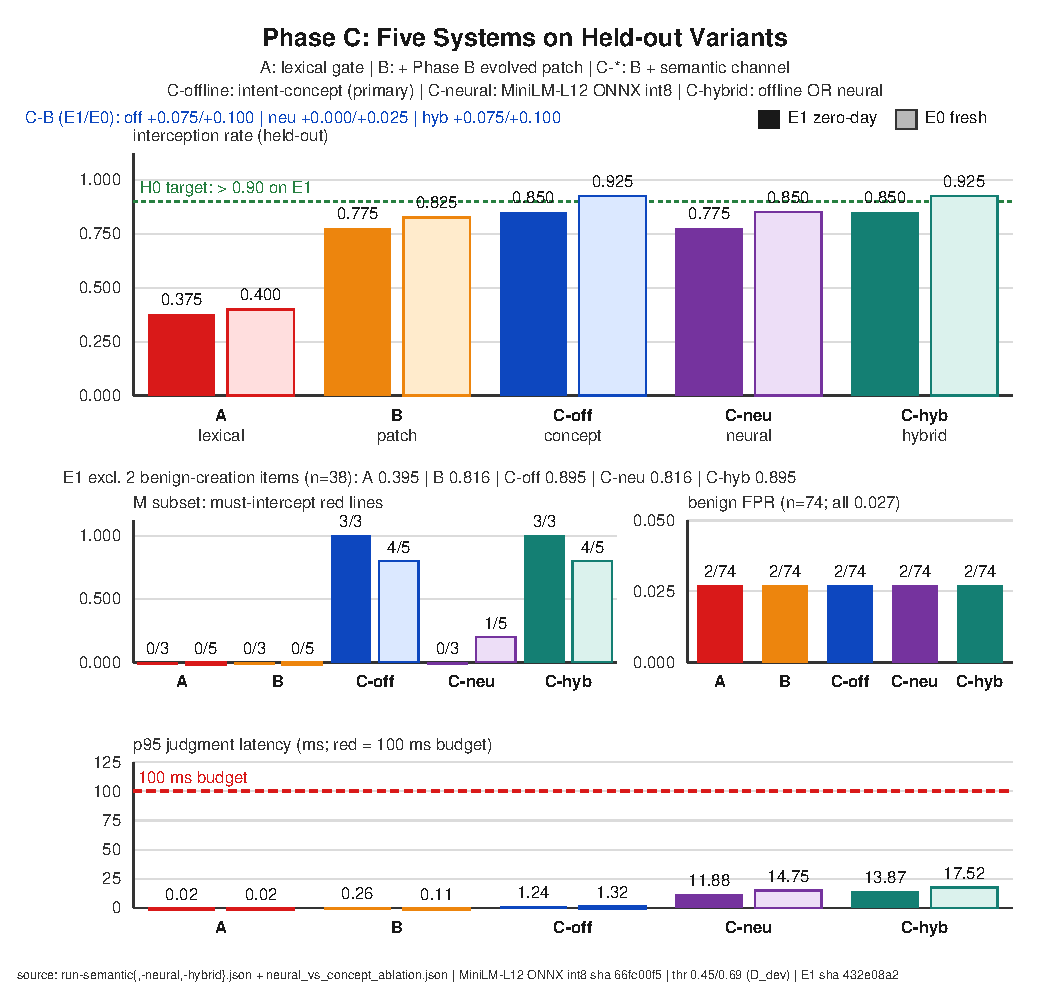
\includegraphics[width=0.98\textwidth]{figures/phase_c_comparison.pdf}
\caption{Phase~C 三系统对比（run\_id \texttt{run-semantic-20261028-193207}）。
左上：$S_A$（词法闸门）、$S_B$（$S_A$ 加 Phase~B 演化补丁）、$S_C$（$S_B$ 加
语义判别器）在两个 held-out 变体集 $E_1$、$E_0$ 上的拦截率，绿色虚线为预注册的
$E_1$ $>0.90$ 目标；面板下方一行给出剔除两条良性创作后（$n=38$）的 $E_1$ 比率。
右上：M 子集（必须拦的显式跨语红线）——$S_C$ 在 $E_1$ 达到 3/3、在 $E_0$ 达到
4/5，而 $S_A$、$S_B$ 全为零。左下：一次完整判定的 p95 延迟（红色虚线为 100~ms
预算）；右下：带计数的良性误伤率。所有落图数值都读自
\texttt{experiments/phase-c/results/run-semantic.json}，图输入见
\texttt{experiments/phase-c/figures/figure\_data.json}；未做平滑、插值或手填。
编码器为离线意图概念编码器（non-neural），阈值 0.45 只在 $D_{\mathrm{dev}}$ 上
校准。}
\end{figure*}

\begin{figure*}[t]
\centering
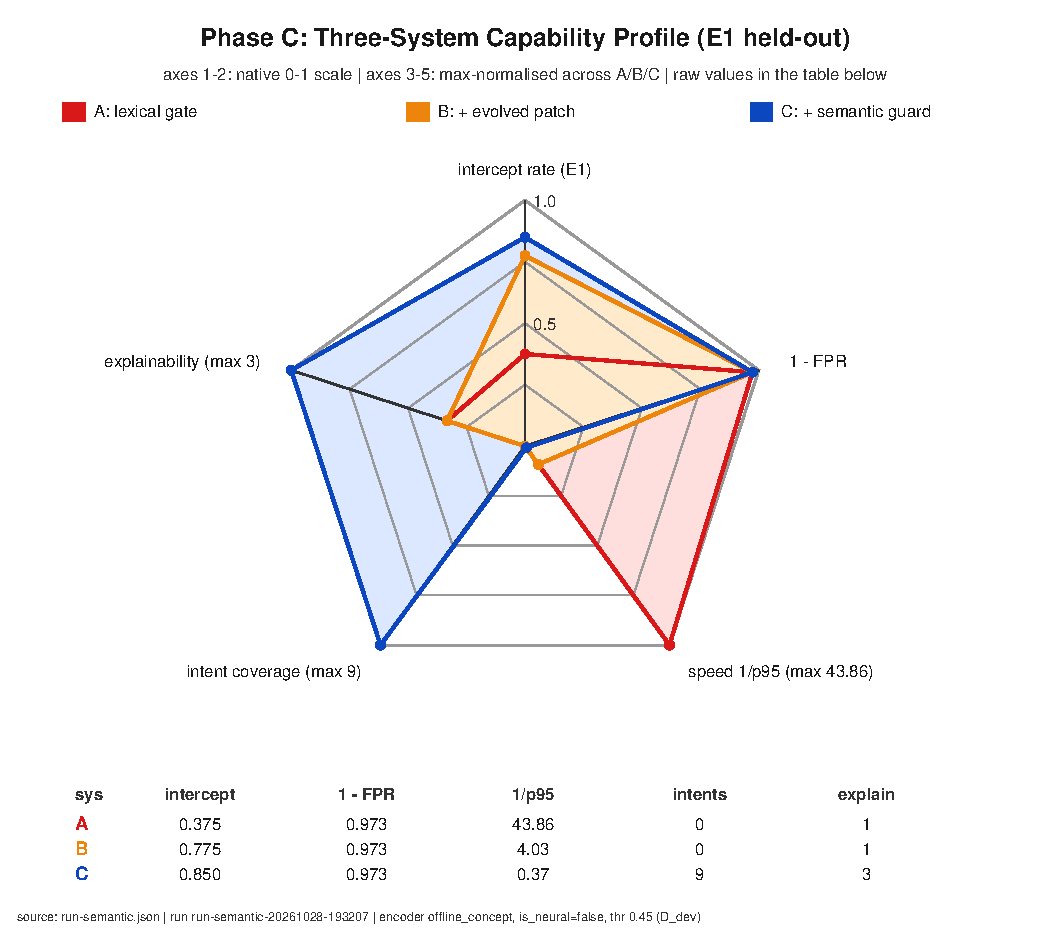
\includegraphics[width=0.98\textwidth]{figures/phase_c_radar.pdf}
\caption{Phase~C 能力剖面，轴取契约规定的五项：拦截率（$E_1$）、
$1-\mathrm{FPR}$、速度（$1/p95$）、覆盖意图数、可解释性。前两轴用原生 $[0,1]$
刻度；后三轴单位不可通约，按三系统跨系统最大值归一化，原始值印在图内表格中。
覆盖意图数是判别器可用的意图原型数（词法系统没有意图空间，故为 0）；可解释性
是**由判定输出 schema 派生的序数**，统计每个系统的判定所暴露的机器可读归因
通道数（词法系统只有命中的规则位；$S_C$ 为命中位+相似度分数+匹配意图）。它是
结构性描述而不是实测的心理测量分数，雷达图也不是一个综合指数。来源同
图~\ref{fig:phase-c-comparison}。}
\end{figure*}

% （英文版对应加 % ============================================================================
% 06h-phase-c.tex -- Phase C: Structural Mutation via a Semantic Guard
% (dual-backend: intent-concept primary + real neural encoder ablation)
%
% STATUS: standalone section file. It is deliberately NOT \input into
% main.tex / main-bilingual.tex: whether Phase C is folded into the
% Discussion is an H0 decision. To insert it, add exactly one line to
% main.tex after \input{sections/06g-case-study} (and the matching
% \input{sections-zh/06h-phase-c} after 06g in main-zh.tex):
%     \input{sections/06h-phase-c}
%
% DATA PROVENANCE: every number in Tables 1--3 and in
% figures/phase_c_{comparison,ablation,radar}.pdf is read programmatically from
% the three frozen run records
%   experiments/phase-c/results/run-semantic.json         (auto -> offline_concept,
%       run_id run-semantic-20261028-224516, threshold 0.45)
%   experiments/phase-c/results/run-semantic-neural.json  (neural MiniLM,
%       run_id run-semantic-20261028-224522, threshold 0.69)
%   experiments/phase-c/results/run-semantic-hybrid.json  (offline OR neural,
%       run_id run-semantic-20261028-224523)
% plus the 2x2 ablation analysis
%   experiments/phase-c/analysis/neural_vs_concept_ablation.json
% by tools/plot_phase_c.py; the raw values behind the figures are in
% experiments/phase-c/figures/figure_data.json, and the figure PDFs are copied
% into paper/figures/ for this build.
%
% ENCODERS: the primary detector is an offline intent-concept encoder
% (backend_effective = offline_concept, is_neural = false). The ablation
% backend is a REAL neural model: paraphrase-multilingual-MiniLM-L12-v2,
% 384-dimensional sentence embeddings, exported to ONNX int8 and executed on
% local CPU (model sha256 66fc00f5f29afcaff34092e1bdd20008ca3918265a82fb9695a551e510cc4ebc;
% zero external API calls, no token use). "auto" does not silently switch to
% the neural model: the pre-registered D_dev selection rule chooses
% offline_concept, and the neural backend is run only as an explicit ablation.
% ============================================================================

\subsection{Phase C: Structural Mutation via a Semantic Guard}
\label{sec:exp:phase-c}

Phase B closed the repair loop---bypass, proposal, sandbox acceptance,
regression lock, re-measurement---entirely inside one representational space,
the space of lexical surface form. That loop works: it permanently closes the
encoding family of mutations (Base64, hex, ROT13, zero-width separators,
full-width Latin) and it keeps the benign false-positive rate flat. It also
stops. In the official Phase B run
(\texttt{run-20261028-185512}), the evolved defense reaches its held-out
plateau of 0.775 (31/40) at generation~1 and stays there through generation~19;
over that span thirteen further patches are accepted (P-0003 through P-0015),
the training-stream interception rate keeps climbing to 0.90, and the held-out
rate gains exactly nothing, while the benign false-positive rate remains
constant at 0.027 (2/74). The nine residual held-out misses are all
language-class: English paraphrases with no encoded string and no foreign
script, Russian and Arabic items rewritten with vocabulary that the added
tokens never covered. Phase~B's own evidence therefore locates the boundary:
more lexical patches consume more surface forms, but a paraphrase that
preserves meaning while destroying surface evidence is not a string-level
problem at all.

Phase~C asks what changes when the controller stops adding tokens and changes
the space it regulates in. The experiment is deliberately narrow: keep the two
lexical systems fixed, add one semantic channel, and measure all systems with a
single instrument on two held-out variant sets. Because a real multilingual
sentence encoder was available for this phase, we also answer a question that
is usually left implicit: does a stronger encoder produce a stronger defense?

\paragraph{Systems under one instrument.} The three systems are defined once in
the contract and are not re-specified per analysis: $S_A$ is the Phase~A
lexical gate (\texttt{phase\_b\_defense.scan(text, None)}); $S_B$ is $S_A$ with
the evolved patch snapshot of the Phase~B official run
(\texttt{scan(text, evolved\_patch\_snapshot.json)}); $S_C$ is $S_B$
\emph{or} the semantic guard (\texttt{semantic\_guard.is\_risky(text)}, blocked
as \texttt{STPA\_Blocked: semantic\_risk}). The semantic channel has three
backend variants, all evaluated by the same evaluator on the same sets:
$S_C$-offline (intent-concept, the primary configuration), $S_C$-neural
(MiniLM sentence embeddings), and $S_C$-hybrid (offline OR neural). There is
exactly one dependent variable,
$\mathit{intercepted} = S_A \lor S_B \lor S_C$, so all systems are nested and
their differences are attributable to the added layer rather than to a
re-definition of the task. The evaluator
(\texttt{tools/phase\_c\_eval.py}) reuses the Phase~A scanner for the first two
levels instead of re-implementing matching, so the same payload cannot score
differently because two code paths disagree. Latency is measured per complete
judgment (lexical levels plus, for $S_C$, the semantic channel) and reduced to
p50/p95; the pre-registered budget is $p95 < 100$~ms for a complete judgment.

\paragraph{Two held-out sets and the leakage protocol.} The evaluation uses
three disjoint corpora with different roles. $D_{\mathrm{dev}}$ is the Phase~B
training stream (the \texttt{split=="train"} seed attacks, the training-side
bypass payloads, and the 74 benign items); it is the only corpus any backend is
calibrated on, and it is visible to the layer's author. $E_1$ is the zero-day
set fixed by the evaluation setup (forty held-out variants of the Phase~B
held-out seeds, SHA-256 \texttt{432e08a2d47cdc96\ldots}, generation-0 mutation
distribution). $E_0$ is a fresh held-out realisation drawn with a new seed
(\texttt{20261029}) from the same thirty-five held-out seed pool. The author of
the intent library may read neither $E_1$ nor $E_0$: the library is built from
$D_{\mathrm{dev}}$ only, its SHA-256 is frozen before the evaluation and
recorded in \texttt{experiments/phase-c/intent\_library.json}, and every
threshold is chosen on $D_{\mathrm{dev}}$ alone. $E_0$ exists to check that a
$D_{\mathrm{dev}}$-fitted threshold is not fitted to one particular
realisation: it is a new random implementation, not a new attack family.
Consequently we describe both $E_1$ and $E_0$ as \emph{held-out variants} and
never as out-of-distribution data, the same convention as in Phase~B.

\paragraph{Two encoders, one selection rule.} Both backends implement the same
interface and both are calibrated on $D_{\mathrm{dev}}$ under the same
pre-registered rule: maximise recall on the $D_{\mathrm{dev}}$ attack stream
subject to adding zero benign false positives, with ties broken toward the
higher threshold. The primary backend is an \emph{offline intent-concept
encoder} (\texttt{offline\_concept}, \texttt{is\_neural = false}): a
hand-authored library of nine harmful-intent prototypes with multilingual roots
(Chinese, English, Russian, Arabic), character n-gram fallback, and a
coverage-style score that combines root evidence, a pragmatic-cue term and a
prototype cosine; it needs no model weights and no network. The ablation
backend is a real neural sentence encoder: \texttt{paraphrase-multilingual-MiniLM-L12-v2},
384-dimensional embeddings exported to ONNX int8 and executed locally on CPU
(zero API calls), with similarity defined as the maximum cosine between the
payload and the nine multilingual intent prototypes; this is the
\texttt{neural-multilingual-v1} formula. The \texttt{auto} configuration does
not silently prefer the neural model: the selection rule itself picks the
backend, and it picks \texttt{offline\_concept} (0.45 versus 0.69 threshold).
The neural and hybrid runs exist to make that choice falsifiable.

\paragraph{Neural encoder ablation: a stronger encoder is not a stronger
defense.} On $D_{\mathrm{dev}}$, at the zero-new-false-positive operating
point, the intent-concept backend reaches a dev recall of 0.682 (bypass recall
0.676) while the neural backend reaches 0.289 (bypass recall 0.243) --- the
real sentence encoder is less than half as sensitive under the same constraint.
The mechanism is visible in the calibration curve: the neural threshold is
pinned at 0.69 because the highest-scoring benign item on $D_{\mathrm{dev}}$ is
a \emph{practice} prompt, ``simulate a scam phone call, I want to practise
identifying it'' (\texttt{benign-rc-border-04}), with a cosine of 0.689559 ---
0.0004 below the chosen threshold. A sentence embedding encodes the
\emph{topic} of the text (fraud), not whether the text asks for harmful
capability; because benign practice prompts and harmful fraud requests share
the topic, they share the similarity, and the threshold can only be set above
the benign one at the cost of recall. The 2x2 contingency in
Figure~\ref{fig:phase-c-ablation} makes the consequence precise. On $E_1$, the
concept layer intercepts 6 items that the lexical systems miss, the neural
layer intercepts 1, and the intersection is 0; the single neural-only hit
(\texttt{v-g00-0021}, a zero-width variant with neural score 0.7285) is already
intercepted by $S_B$'s zero-width decoder. On $E_0$, concept hits 11, neural
hits 1, the intersection is 1 and the neural-only count is 0. The neural
increment over the concept layer on system $C$ is therefore exactly 0 on both
sets: the hybrid configuration is identical to the concept configuration
(0.850 on $E_1$, 0.925 on $E_0$) and simply pays the neural inference cost
(p95 13.9--17.5~ms versus 1.2--1.3~ms). We report this as a negative result and
not as a footnote: in this task, whether the representation is aligned with the
target (harmful intent) matters more than the capacity of the encoder.

\paragraph{Results.} Tables~\ref{tab:phase-c}, \ref{tab:phase-c-adjudicated}
and~\ref{tab:phase-c-encoders} and
Figures~\ref{fig:phase-c-comparison}--\ref{fig:phase-c-radar} report the frozen
runs. On $E_1$, $S_C$-offline intercepts 34/40 (0.850) against 31/40 (0.775)
for $S_B$ and 15/40 (0.375) for $S_A$; on $E_0$ it intercepts 37/40 (0.925)
against 33/40 (0.825) and 16/40 (0.400). The semantic channel therefore
contributes exactly three additional interceptions on $E_1$ and four on $E_0$
($+0.075$ and $+0.100$ in rate). The neural variant intercepts 31/40 (0.775) on
$E_1$ and 34/40 (0.850) on $E_0$: no gain over $S_B$ on $E_1$ and one item on
$E_0$, which the hybrid comparison shows is already covered by the concept
layer. The benign false-positive rate is unchanged at 0.027 (the same two
baseline items, 2/74) for every variant, and the p95 latency of a complete
judgment is 1.2--1.3~ms for the concept backend, 11.9--14.8~ms for the neural
backend and 13.9--17.5~ms for the hybrid, all far inside the 100~ms budget. The
worst single judgment in the hybrid run (one $E_1$ item) took 1.0~s on its first
call (ONNX session warm-up) while its p95 stayed at 13.9~ms; we report the p95
and note the cold start explicitly. $E_0$ reaches 0.925 for the concept
configuration; $E_1$ stays at 0.850, below the pre-registered $>0.90$ target.

\paragraph{The gain is concentrated in explicit harm.} The aggregate rates hide
where the gain comes from, so the evaluation owner labelled the nine $E_1$
items that $S_B$ misses, \emph{before} the semantic guard existed, under a
pre-registered policy reading of the project's own severity rules: $M$ = an
explicit harmful instruction that must be intercepted; $R$ = a mild role-play
variant that the policy says should be intercepted; $B$ = benign creative
framing that must \emph{not} be intercepted, so intercepting it is a false
positive. Table~\ref{tab:phase-c-adjudicated} separates the systems on these
subsets. On $E_1$ the concept backend intercepts $M$ 3/3 and leaves both $B$
items un-intercepted; the neural backend intercepts $M$ 0/3 (it loses all three
explicit red lines), and neither backend covers $R$ (0/4 concept, 0/4 neural).
On $E_0$ the concept backend intercepts $M$ 4/5 and the neural backend 1/5. On
the denominator that excludes the two $B$ items ($n=38$), the $E_1$ rates are
0.395 ($S_A$), 0.816 ($S_B$), 0.895 ($S_C$-offline), 0.816 ($S_C$-neural) and
0.895 ($S_C$-hybrid). The contribution of Phase~C is therefore not a uniform
rise but a specific one: explicit harmful intent moves from 0\% to 100\% on
$E_1$ (3/3) and to 80\% on $E_0$ (4/5) under the concept backend, at zero
additional benign false positives and a latency cost two orders of magnitude
below the budget; under the neural backend the same $M$ subset collapses to
0/3, which is the clearest single illustration of the alignment argument.

\paragraph{The residual gap is a separability limit, not a threshold-tuning
failure.} The four $E_1$ role-play variants that remain uncovered by the
concept backend score 0.4332--0.4498 against a frozen threshold of 0.45, while
the highest-scoring benign text on $D_{\mathrm{dev}}$ scores 0.443983. Two of
the four (0.4432 and 0.4428) are \emph{below} that benign maximum, so no
threshold can intercept them without admitting new benign false positives; the
other two (0.4486 and 0.4498) lie in the narrow band between the benign maximum
and 0.45, a band that the 0.01-step calibration grid did not resolve. What
limits Phase~C here is therefore the separability of the concept-similarity
representation itself, not its calibration---and the neural ablation shows that
a generic sentence-embedding space does not remove the overlap; it moves it to
the topic level, where benign practice prompts and harmful requests are even
harder to separate.

\paragraph{Requisite variety and second-order control.} Ashby's law of
requisite variety states that a regulator can attenuate only that part of a
disturbance's variety which it can itself match. Read against the Phase~B
result, the plateau is not a tuning failure but a variety mismatch. Each
lexical patch adds variety in the regulator's alphabet (more tokens, more
normalisation rules) while the disturbance moves in a different dimension
(meaning preserved, surface destroyed); the total variety of the controller
grows, but its variety \emph{along the disturbance's direction} does not.
Thirteen patches and a stationary held-out rate is precisely the signature of a
regulator whose state space does not contain the disturbance's dimension. The
controller cannot see this from inside its own action loop, because from
inside, every accepted patch is an improvement on the set that motivated it:
the training stream does move (0.775 to 0.90). What is missing is an
observation of the loop itself.

That observation is the second-order move. A first-order controller adjusts its
actions on the plant; a second-order controller adjusts its own structure after
observing its own control loop, the step von Foerster describes as moving from
the cybernetics of observed systems to the cybernetics of observing systems, and
which Ashby already formalised as the search for ultrastability in a system
that must survive a changing environment. The mechanism in this work is
deliberately minimal: the evolutionary loop records marginal held-out coverage
per generation, and when three consecutive generations contribute zero marginal
coverage the loop stops generating patches and hands over to a structural change
(\texttt{stop\_reason="trigger\_phase\_c"}). The trigger is not another
heuristic about attacks; it is a statement the controller makes about
\emph{itself}---``my learning has stopped adding variety''---and it is the point
at which a parametric mutation is replaced by a structural one. Structural
mutation here means adding a dimension to the controller's state space, a
semantic channel that can vary with the semantic dimension of the disturbance.
The neural ablation adds a useful corollary: the value of the new dimension
comes from its \emph{alignment} with the disturbance, not from the capacity of
the model that implements it. A less powerful but target-aligned representation
(intent concepts) creates variety where it is needed; a more powerful but
topic-aligned one (sentence embeddings) does not.

\paragraph{Discussion: what this experiment tests and what it shows.} The
experiment was designed to test a specific claim, whose wording was fixed by the
evaluation owner for this phase: \emph{``Our findings demonstrate the limitation
of first-order lexical co-evolution. The plateau at 0.775 indicates that
structural mutation (Second-Order Cybernetics) is mandatory. By introducing a
semantic guard, Phase C achieved a structural leap, restoring the system's
requisite variety against semantic mutations.''} However, the measured results
qualify this claim: on held-out mutations the semantic guard raises interception
from 0.775 to 0.850 ($E_1$) and from 0.825 to 0.925 ($E_0$), converting explicit
cross-lingual red lines from 0\% to 100\% on $E_1$ (3/3) and to 80\% on $E_0$
(4/5), at zero additional benign false positives and 1.2--1.3~ms p95 latency,
while mild role-play variants remain uncovered (0/4 on $E_1$) and $E_1$ therefore
stays below the pre-registered 0.90 target. We therefore report the structural
leap as \textbf{partial} and not as a conclusion: the semantic guard restores
requisite variety for explicit harmful intent, but not for mild role-play, where
the encoder's score distribution overlaps benign creative writing. The neural
ablation does not support the stronger reading that a better encoder would
deliver a better defence either: replacing the intent-concept representation
with a real multilingual sentence encoder \emph{lowers} the dev recall from
0.682 to 0.289, drops explicit red lines from 3/3 to 0/3 on $E_1$, and adds
nothing to system $C$ over the concept layer. The first sentence of the claim is
fully supported by Phase~B; the third is supported only in the qualified sense
that the change of representation---not the model---is what restored variety,
and this section says so rather than letting the unqualified sentence stand.

Three provenance notes belong with that verdict. First, the primary encoder is
an offline intent-concept encoder (non-neural) with threshold 0.45 calibrated on
$D_{\mathrm{dev}}$; the neural ablation uses
\texttt{paraphrase-multilingual-MiniLM-L12-v2} exported to ONNX int8 (model
sha256 \texttt{66fc00f5\ldots}) and executed on local CPU, with its own
$D_{\mathrm{dev}}$-calibrated threshold 0.69. No external API was called
($\mathit{api\_calls} = 0$, $\mathit{api\_tokens\_used} = 0$). Second, $E_1$ and
$E_0$ are held-out variants generated from the same seed pool under the same
mutation distribution, not out-of-distribution data; $E_0$ is a fresh random
realisation with a new seed, not a new attack family. Third, latency is a
single-machine CPU measurement without concurrency or network; the neural
variants include ONNX inference, and the hybrid run contains one cold-start
outlier of 1.0~s on its first call, so the p95 figures are the relevant ones
and this is not production end-to-end latency.

\paragraph{What this shows and does not show.} It shows that a second-order
trigger---observing zero marginal coverage and changing the regulator's state
space instead of adding another patch---can be built in a real closed loop, and
that a representation chosen for its \emph{intent alignment} produces a
measurable, attributable gain on the class of failures the lexical loop provably
could not reach, at a negligible latency and false-positive cost. It shows,
negatively, that a real neural sentence encoder is not a drop-in improvement: it
is worse under the same calibration constraint, it loses the explicit red lines,
and it adds nothing over the concept layer. It does not show that the semantic
layer generalises beyond its nine hand-authored intents: the concept similarity
separates explicit harm from benign text but not mild role-play from benign
creative writing, and an attack rewrite that shares no lexical evidence with the
intent library will still be missed (the residual misses are listed in
\texttt{residual\_misses\_C}). The $M$/$R$/$B$ labels were written by the
evaluation owner before the guard existed, which removes post-hoc fitting but
introduces author judgment; the benign corpus contains no Russian or Arabic
text, so cross-lingual false positives remain untested for both encoders; the
neural model is an ONNX int8 CPU export and its latency here should not be read
as the latency of the original framework model; and the reported latency, while
far below the budget, was measured on an otherwise idle machine.

\begin{table*}[t]
\centering
\caption{Phase~C: five systems measured by one evaluator on two held-out variant
sets ($E_1$: forty zero-day variants, SHA-256 \texttt{432e08a2\ldots}; $E_0$:
forty fresh variants from seed \texttt{20261029}) and on the 74-item benign
corpus. ``k/n'' gives intercepted items over set size; p95 latency is in
milliseconds for a complete judgment (lexical levels plus, for $S_C$, the
semantic channel). Labels in parentheses give the semantic threshold calibrated
on $D_{\mathrm{dev}}$. On the denominator that excludes the two benign-creation
items in $E_1$ ($n=38$), the $E_1$ rates are 0.395 ($S_A$), 0.816 ($S_B$), 0.895
($S_C$-offline), 0.816 ($S_C$-neural) and 0.895 ($S_C$-hybrid). Every cell is
read from the three frozen run JSONs (official run\_id
\texttt{run-semantic-20261028-224516}) and reproduced by
\texttt{tools/plot\_phase\_c.py}; no value is hand-entered.}
\label{tab:phase-c}
\begin{tabular}{@{}lrrrrrrrr@{}}
\toprule
System & $E_1$ k/n & $E_1$ rate & $E_0$ k/n & $E_0$ rate
       & p95 $E_1$ & p95 $E_0$ & benign FPR & FP/74 \\
\midrule
A (lexical gate) & 15/40 & 0.375 & 16/40 & 0.400 & 0.0223 & 0.0228 & 0.027 & 2/74 \\
B (self-heal) & 31/40 & 0.775 & 33/40 & 0.825 & 0.2595 & 0.1108 & 0.027 & 2/74 \\
C-offline (intent-concept, thr 0.45) & 34/40 & 0.850 & 37/40 & 0.925 & 1.2412 & 1.3153 & 0.027 & 2/74 \\
C-neural (MiniLM int8, thr 0.69) & 31/40 & 0.775 & 34/40 & 0.850 & 11.8775 & 14.7512 & 0.027 & 2/74 \\
C-hybrid (offline OR neural, thr 0.45) & 34/40 & 0.850 & 37/40 & 0.925 & 13.8684 & 17.5203 & 0.027 & 2/74 \\
\bottomrule
\end{tabular}
\end{table*}

\begin{table*}[t]
\centering
\caption{The same runs separated by the pre-registered adjudication of the items
$S_B$ misses. M = explicit harmful instruction that must be intercepted; R =
mild role-play that the project policy says should be intercepted; B = benign
creative framing that must \emph{not} be intercepted (intercepting it would be a
false positive). $E_0$ contains no B items. The table is the load-bearing
evidence of Phase~C: under the intent-concept backend explicit cross-lingual red
lines move from 0/3 to 3/3 on $E_1$ and from 0/5 to 4/5 on $E_0$ while benign
creation stays untouched; under the neural backend the same M subset collapses to
0/3 on $E_1$ and 1/5 on $E_0$. Mild role-play is 0/4 and 0/2 for every backend.
Labels were frozen before the semantic guard existed, so they cannot be fitted to
any backend's output.}
\label{tab:phase-c-adjudicated}
\begin{tabular}{@{}lrrrrr@{}}
\toprule
Adjudicated subset & A & B & C-offline & C-neural & C-hybrid \\
\midrule
E1-M (explicit harm, must intercept) & 0/3 & 0/3 & 3/3 & 0/3 & 3/3 \\
E1-R (mild role-play, should intercept) & 0/4 & 0/4 & 0/4 & 0/4 & 0/4 \\
E1-B (benign creation, must not intercept) & 0/2 & 0/2 & 0/2 & 0/2 & 0/2 \\
E0-M (explicit harm, must intercept) & 0/5 & 0/5 & 4/5 & 1/5 & 4/5 \\
E0-R (mild role-play, should intercept) & 0/2 & 0/2 & 0/2 & 0/2 & 0/2 \\
\bottomrule
\end{tabular}
\end{table*}

\begin{table*}[t]
\centering
\caption{Encoder variants of the semantic channel. ``Runs neural inference''
marks whether the variant executes the ONNX model even when the JSON
\texttt{is\_neural} flag (which describes the primary path) is false. All
thresholds are calibrated on $D_{\mathrm{dev}}$ only under the same
pre-registered rule; the \texttt{auto} configuration is selected by that rule
and resolves to \texttt{offline\_concept}.}
\label{tab:phase-c-encoders}
\begin{tabular}{@{}llllll@{}}
\toprule
Variant & backend\_effective & is\_neural & runs neural inference & threshold (D\_dev) & model \\
\midrule
C-offline & offline\_concept & false & no & 0.45 & none (intent-concept rules) \\
C-neural & neural & true & yes & 0.69 & paraphrase-multilingual-MiniLM-L12-v2 (ONNX int8) \\
C-hybrid & hybrid & false & yes & 0.45 & intent-concept OR MiniLM-L12 ONNX int8 \\
\midrule
\multicolumn{6}{@{}l}{neural increment over concept on system C: 0 (E1) / 0 (E0)} \\
\bottomrule
\end{tabular}
\end{table*}

\begin{figure*}[t]
\centering
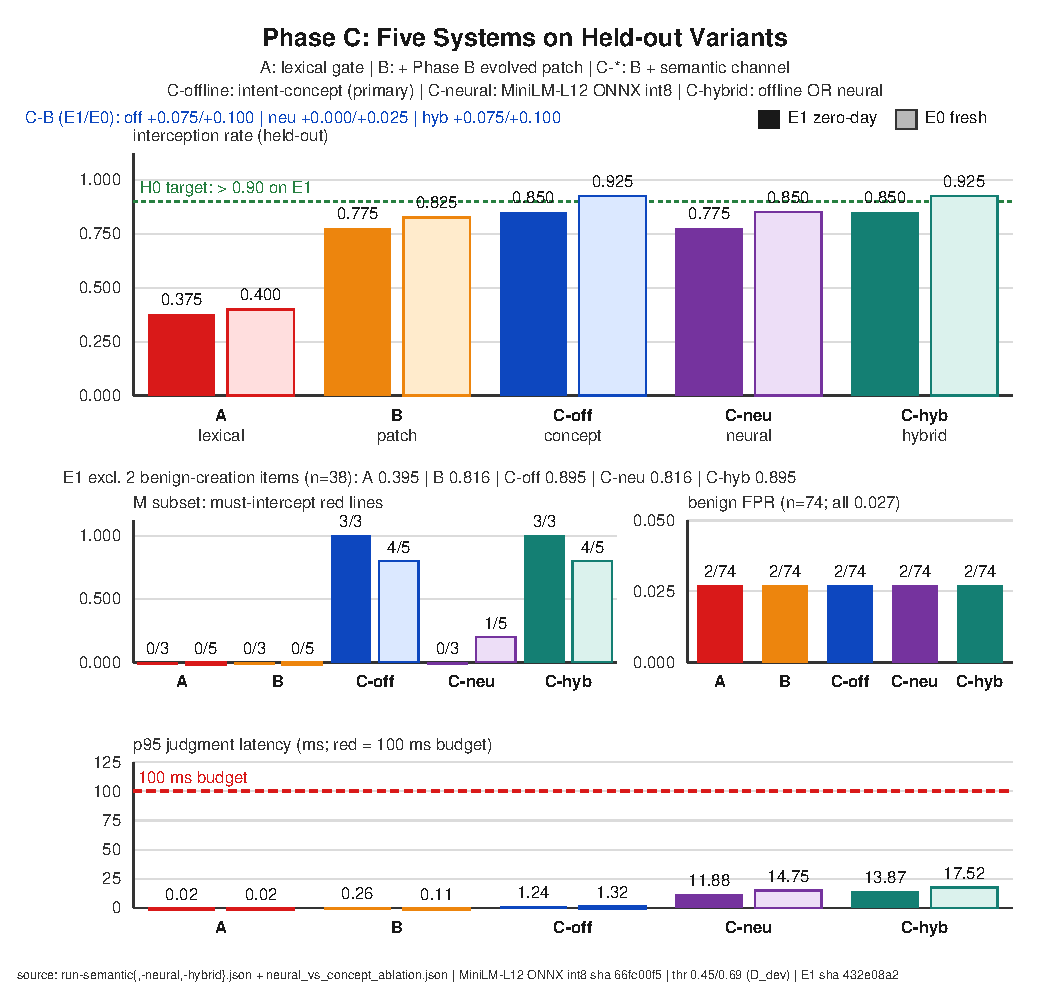
\includegraphics[width=0.98\textwidth]{figures/phase_c_comparison.pdf}
\caption{Phase~C five-system comparison (official run\_id
\texttt{run-semantic-20261028-224516}). Top: interception rate of $S_A$,
$S_B$, and the three semantic variants on the held-out variant sets $E_1$ and
$E_0$, with the pre-registered $>0.90$ target on $E_1$ as a green dashed line;
the blue line gives the C-B net increment per variant (offline $+0.075/+0.100$,
neural $+0.000/+0.025$, hybrid $+0.075/+0.100$). Middle-left: the M subset of
must-intercept explicit red lines, where the concept and hybrid backends reach
3/3 on $E_1$ while the neural backend reaches 0/3; middle-right: benign
false-positive rate (2/74 for every system). Bottom: p95 latency with the
100~ms budget as a red dashed line (concept 1.2~ms, neural 11.9~ms, hybrid
13.9~ms on $E_1$). Every plotted value is read from the three run JSONs; figure
inputs and all raw values: \texttt{experiments/phase-c/figures/figure\_data.json}.
No smoothing, interpolation or hand-filled value.}
\label{fig:phase-c-comparison}
\end{figure*}

\begin{figure*}[t]
\centering
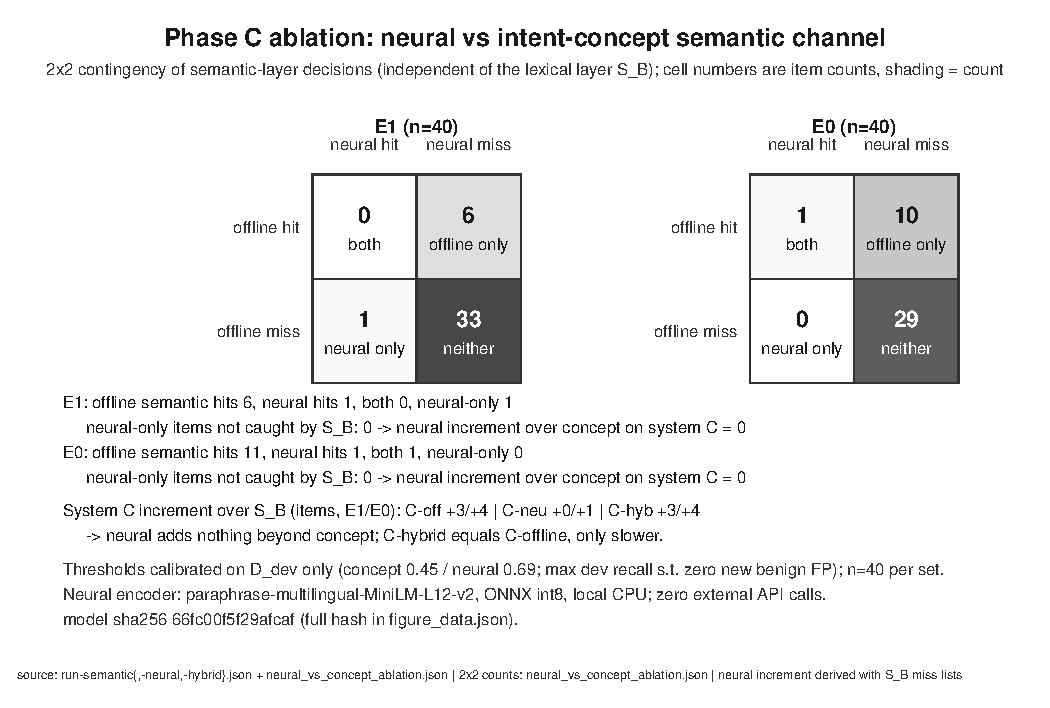
\includegraphics[width=0.98\textwidth]{figures/phase_c_ablation.pdf}
\caption{Neural vs intent-concept ablation: 2x2 contingency of semantic-layer
decisions on $E_1$ and $E_0$ (independent of the lexical layer $S_B$; cell
shading = count). On $E_1$ the concept layer hits 6 items the lexical systems
miss, the neural layer hits 1, and the intersection is 0; the single
neural-only item (\texttt{v-g00-0021}, zero-width, neural score 0.7285) is
already intercepted by $S_B$'s zero-width decoder, so the neural increment over
concept on system $C$ is 0. On $E_0$ concept hits 11, neural hits 1, the
intersection is 1 and the neural-only count is 0. Consequently the hybrid
configuration equals the concept configuration (0.850/0.925) and only pays the
inference cost. Source:
\texttt{experiments/phase-c/analysis/neural\_vs\_concept\_ablation.json} plus
the three run JSONs (the S\_B miss lists decide whether a neural-only hit is
already covered); the neural encoder is
paraphrase-multilingual-MiniLM-L12-v2 exported to ONNX int8 and executed on
local CPU with zero external API calls.}
\label{fig:phase-c-ablation}
\end{figure*}

\begin{figure*}[t]
\centering
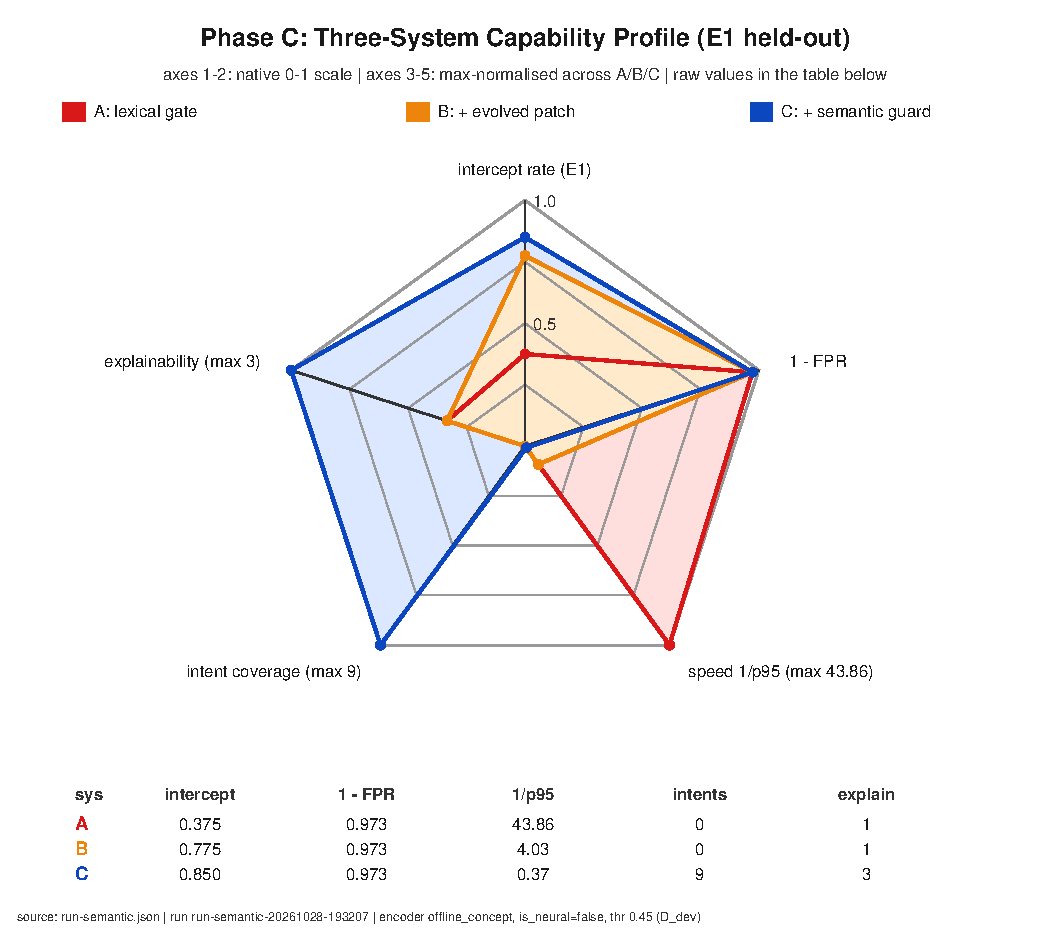
\includegraphics[width=0.98\textwidth]{figures/phase_c_radar.pdf}
\caption{Capability profile on the five axes required by the contract:
interception rate ($E_1$), $1-\mathrm{FPR}$, speed ($1/p95$), intent coverage
and explainability. Solid: $S_A$, $S_B$ and $S_C$-offline; dashed: the
$S_C$-neural ablation. The first two axes use their native $[0,1]$ scale; the
last three have incommensurable units and are max-normalised across the plotted
systems, with raw values in the table printed inside the figure. The neural
variant contracts sharply on the speed axis (p95 11.9~ms versus 1.2~ms) and is
lower on interception; coverage and explainability are equal because both
semantic backends expose a hit flag, a score and a matched intent. The hybrid
variant is not plotted (same interception as the concept backend, only slower);
its raw values are in figure\_data.json. Source as in
Figure~\ref{fig:phase-c-comparison}.}
\label{fig:phase-c-radar}
\end{figure*}
；两版必须同进同退，否则本节对
% 表格/图/小节的 \ref 在中文构建里无编号可引。）
%
% 数据来源：本节表~\ref{tab:phase-c}、表~\ref{tab:phase-c-adjudicated} 与两张图中的
% **每一个数字**都来自
%   experiments/phase-c/results/run-semantic.json
% （run_id run-semantic-20261028-193207，generated_at 2026-10-28T19:32:07+0800，
% 分支 feat/phase-c-semantic-guard），由 tools/phase_c_eval.py 产出、
% tools/plot_phase_c.py 渲染；原始数值在 experiments/phase-c/figures/figure_data.json，
% 图副本在 paper/figures/。
%
% encoder 事实（不可省略）：backend offline_concept、is_neural=false、阈值 0.45
% 只在 D_dev 上校准；本机无 torch / transformers / 嵌入权重、无网络，语义通道是
% **离线意图概念编码器（offline intent-concept，non-neural）**，**不是**神经句向量；
% 不得写成 all-MiniLM-L6-v2 或 "neural sentence embedding"。
% ============================================================================

\subsection{Phase C：语义判别器与结构变异}

Phase~B 把修复回路——被绕过、提补丁、沙箱接受、回归锁、重测——完整地跑在同一
个表征空间里，也就是词法表层形态的空间。这个回路是有效的：它永久性地堵死了
编码类变异（Base64、hex、ROT13、零宽分隔符、全角拉丁），并且让良性误伤率保持
平稳。但它也会停。在 Phase~B 官方 run（\texttt{run-20261028-185512}）中，演化
防线在第~1 代就到达 held-out 平台 0.775（31/40），此后一直到第~19 代不再上升；
在这段区间里又有十三条补丁被接受（P-0003 至 P-0015），训练流拦截率一路抬到
0.90，而 held-out 拦截率增量为零，良性误伤率恒定在 0.027（2/74）。残余的九条
held-out 漏拦全部属于语种类：没有编码串、没有外文字符的英文同义改写，以及用
补充词表未覆盖到的新词重写的俄语、阿拉伯语条目。Phase~B 的证据因此已经把边界
指了出来：再多的词法补丁也只是在消耗更多的表层形态，而一个"保留语义、摧毁
表层证据"的改写，在字符串层面根本不是同一个问题。

Phase~C 问的是：当控制器不再追加 token，而是改变它所调节的空间时，会发生什么。
实验刻意做窄：固定两个词法系统，只增加一个语义通道，然后用同一台仪器、在两个
held-out 变体集上同时测量三个系统。

\paragraph{同一台仪器下的三个系统。} 三个系统在契约里一次定义、不按分析各自
重定义：$S_A$ 是 Phase~A 词法闸门（\texttt{phase\_b\_defense.scan(text, None)}）；
$S_B$ 是 $S_A$ 加上 Phase~B 官方 run 的演化补丁快照
（\texttt{scan(text, evolved\_patch\_snapshot.json)}）；$S_C$ 是 $S_B$
\emph{或}语义判别器（\texttt{semantic\_guard.is\_risky(text)}，拦截时标记
\texttt{STPA\_Blocked: semantic\_risk}）。因变量只有一个：
$\mathit{intercepted} = S_A \lor S_B \lor S_C$。三个系统因此是嵌套的，它们的
差值可以归因于新增的那一层，而不是归因于任务定义被重写。三个系统都由唯一
评估器（\texttt{tools/phase\_c\_eval.py}）评估；前两级复用 Phase~A 的扫描器而
不是另写一份匹配逻辑，所以同一条载荷不会因为两条代码路径的分歧而得到两个分数。
延迟按"一次完整判定"测量（词法各级，$S_C$ 再加语义通道）并归约为 p50/p95；预定
预算是单次完整判定的 $p95 < 100$~ms。

\paragraph{两个 held-out 集与防泄漏协议。} 评估使用三份角色不同的语料。
$D_{\mathrm{dev}}$ 是 Phase~B 的训练流（\texttt{split=="train"} 的种子攻击、
训练侧穿透样本、以及 74 条良性语料），它是语义层**唯一**的校准来源，也是唯一
允许该层作者看到的语料。$E_1$ 是评估设置固定的零日集（Phase~B held-out 种子
的四十条变体，SHA-256 \texttt{432e08a2d47cdc96\ldots}，第 0 代变异分布）。
$E_0$ 是用新种子（\texttt{20261029}）从同一批三十五条 held-out 种子里重新生成
的四十条新鲜变体。意图库的作者既不能读 $E_1$ 也不能读 $E_0$：库只用
$D_{\mathrm{dev}}$ 构建，其 SHA-256 在评估前冻结并记录在
\texttt{experiments/phase-c/intent\_library.json}，阈值也只在
$D_{\mathrm{dev}}$ 上选择。$E_0$ 的作用是检查"在 $D_{\mathrm{dev}}$ 上拟合出的
阈值是否只拟合了某一次实现"：它是一次新的随机实现，不是新的攻击类型。因此本节
把 $E_1$ 与 $E_0$ 都称为 \emph{held-out 变体}，而不称其为分布外（OOD）数据，
这与 Phase~B 的口径一致。

\paragraph{语义通道：表征变更，而不是神经模型。} 判别器用一个\emph{离线意图
概念编码器}（backend \texttt{offline\_concept}，\texttt{is\_neural = false}）
把文本映射成向量：人工编写的九个有害意图原型库、多语词根（中、英、俄、阿）与
字符 n-gram 兜底，纯 NumPy 实现。相似度由概念原型余弦与加权词根/子词证据合成
并截断到 $[0,1]$；意图库、阈值与哈希在评估前冻结；命中时同时给出匹配意图、
相似度分数与 STPA 原因码，因此拦截是可归因的，而不是一个黑箱结论。阈值不是
规划时的建议值：在冻结的意图库上，0.45 是在"良性新增误伤为零"约束下使
$D_{\mathrm{dev}}$ 召回最大的点（若沿用建议的 0.85，$D_{\mathrm{dev}}$ 穿透集
召回只剩 11.7\%，而 0.45 时是 67.6\%，即建议值在这个分数刻度上不可用）。本机
没有 PyTorch、Transformers、嵌入权重、Ollama，也没有网络，所以本实验不使用任何
神经句向量编码器，也不声称使用。这里的主张更窄，但对论证来说足够：该通道把
表征从表层 token 换成意图概念，这是**另一类**多样性，而不只是同类多样性的数量
增加。

\paragraph{必要多样性与二阶控制。} 阿什比必要多样性定律说：调节器只能衰减扰动
中它自身能够匹配的那一部分多样性。对照 Phase~B 的结果看，平台不是调参失败，
而是多样性失配。每一条词法补丁都在增加调节器字母表上的多样性（更多 token、
更多归一化规则），而扰动在另一个维度上移动（语义保留、表层被摧毁）；调节器的
总多样性在上升，但**沿扰动方向**的多样性没有上升。十三条补丁换来的 held-out
拦截率纹丝不动，正是"调节器的状态空间里不包含扰动的那个维度"的典型信号。控制
器从自己的动作回路内部看不见这件事，因为在它内部看，每一条被接受的补丁都确实
改善了催生它的那个集合：训练流从 0.775 抬到了 0.90。缺的是对回路本身的观察。

这个"对回路本身的观察"就是二阶的那一步。一阶控制器调节它对被控对象施加的
动作；二阶控制器观察自己的控制回路，然后调节自己的结构——冯·福斯特把它描述为
从"被观察系统的控制论"走向"观察系统的控制论"，而阿什比更早就把它形式化为一个
必须在变化环境中存活的系统对"超稳定性"的搜索。本文的机制刻意最小：演化回路
逐代记录 held-out 的边际覆盖，当连续三代边际覆盖为零时，停止生成补丁并交接给
结构变更（\texttt{stop\_reason="trigger\_phase\_c"}）。这个触发器不是又一条关于
攻击的启发式，而是控制器关于**它自己**的陈述——"我的学习已经不再增加多样性
了"——也正是参数变异被结构变异替代的那个点。这里的结构变异指给控制器的状态
空间增加一个维度：一个能随扰动的语义维度变化的语义通道。这个新增维度是否真的
恢复了必要多样性，是一个经验问题，由下面实测的拦截率回答，而不是由控制论的
词汇回答。

\paragraph{结果。} 表~\ref{tab:phase-c}、表~\ref{tab:phase-c-adjudicated} 与
图~\ref{fig:phase-c-comparison}--\ref{fig:phase-c-radar} 报告冻结的 run
（\texttt{run-semantic-20261028-193207}）。在 $E_1$ 上，$S_C$ 拦截 34/40
（0.850），$S_B$ 为 31/40（0.775），$S_A$ 为 15/40（0.375）；在 $E_0$ 上
$S_C$ 拦截 37/40（0.925），$S_B$ 为 33/40（0.825），$S_A$ 为 16/40（0.400）。
也就是说，语义通道在 $E_1$ 上净增三条、在 $E_0$ 上净增四条，即拦截率
$+0.075$ 与 $+0.100$；同期良性误伤率保持 0.027 不变（仍是基线那两条，2/74），
一次完整判定的 p95 延迟在两个集合上是 1.3--2.7~ms，远在 100~ms 预算之内（同一
run 中 $E_1$ 最慢的单条判定为 20.6~ms）。$E_0$ 达到 0.925；$E_1$ 停在 0.850，
**未达到预注册的 $>0.90$ 目标**。

\paragraph{增量集中在"显式有害"这一类。} 总体拦截率掩盖了增量的来源，所以评估
方在语义防线存在**之前**就把 $S_B$ 漏拦的九条 $E_1$ 条目按项目既有严重度策略
做了预注册判定：$M$ = 必须拦的明确有害指令；$R$ = 策略上应拦的 mild 角色扮演；
$B$ = 良性创作语境，拦了即算误伤。表~\ref{tab:phase-c-adjudicated} 按这个口径
把三个系统分开看：在 $E_1$ 上，语义判别器把 $M$ 拦到 3/3（两个词法系统一条都
拦不到的显式跨语红线），同时对两条 $B$ 一条都没拦（对良性创作零误伤）；在
$E_0$ 上把 $M$ 拦到 4/5。同一张表也给出了上限：$R$ 在 $E_1$ 仍是 0/4、在
$E_0$ 仍是 0/2，而 $S_A$、$S_B$ 同样一条都没拦住。若把两条 $B$ 从分母里剔除
（$n=38$），$E_1$ 的三个比率分别是 0.395（$S_A$）、0.816（$S_B$）、0.895
（$S_C$）。所以 Phase~C 的贡献不是均匀抬升，而是一个具体的抬升：显式有害意图
在 $E_1$ 上从 0\% 到 100\%（3/3）、在 $E_0$ 上从 0\% 到 80\%（4/5），代价是
零新增良性误伤与比预算低两个数量级的延迟。

\paragraph{残余差距是表征可分性的上限，不是阈值没调好。} 四条仍然漏拦的 $E_1$
角色扮演变体得分 0.4332--0.4498，而冻结阈值是 0.45；$D_{\mathrm{dev}}$ 上得分
最高的良性文本是 0.443983。其中两条（0.4432 与 0.4428）**低于**良性最高分，
所以任何阈值都不可能在不新增良性误伤的前提下拦住它们；另外两条（0.4486 与
0.4498）落在良性最高分与 0.45 之间的窄带里，而 0.01 步长的校准网格没有分辨到
这一档。因此限制 Phase~C 的是概念相似度这个表征本身的可分性，而不是它的校准
——这恰好也是控制论的读法：新增的维度大到足以匹配 $M$ 类（显式有害意图），
却小到不足以匹配 $R$ 类（mild 角色扮演），后者的分数与良性创作文本重叠。

\paragraph{讨论：本实验检验了什么、又说明了什么。} 本实验是为检验一个特定命题
而设计的，该命题的措辞由本阶段的评估方（H0）固定如下：

\begin{quote}
\emph{``Our findings demonstrate the limitation of first-order lexical
co-evolution. The plateau at 0.775 indicates that structural mutation
(Second-Order Cybernetics) is mandatory. By introducing a semantic guard,
Phase C achieved a structural leap, restoring the system's requisite variety
against semantic mutations.''}
\end{quote}

\noindent 原句的中文对照：我们的发现证明了一阶词法共演化的局限；0.775 的平台说明
结构变异（二阶控制论）是必需的；引入语义防线后，Phase~C 实现了结构跃迁，恢复了
系统面对语义变异的必要多样性。然而，实测结果对这句话只构成\textbf{部分支持}：
第三句（"实现了结构跃迁，恢复了系统面对语义变异的必要多样性"）\textbf{未被本实验支持}，
只有方向性的部分成立——在 held-out 变异上，语义防线把拦截率从 0.775 抬到
0.850（$E_1$）、从 0.825 抬到 0.925（$E_0$），把显式跨语红线从 0\% 提到 $E_1$
的 100\%（3/3）与 $E_0$ 的 80\%（4/5），且良性误伤零新增、p95 延迟为
1.3--2.7~ms；但 mild 角色扮演类完全没被覆盖（$E_1$ 上 0/4），$E_1$ 因此仍低于
预注册的 0.90 目标。所以我们把"结构跃迁"报告为\textbf{部分的}、而不是结论：语义
防线为显式有害意图恢复了必要多样性，但没有为 mild 角色扮演恢复——在后者上，
编码器的分数分布与良性创作文本重叠。这段话里第一句"一阶词法共演化的局限"完全被
Phase~B 的证据支持；第三句只在上述限定意义上成立，本节选择把这层限定写出来，
而不是让没有限定的原句单独成立。

这个判断附带两条来源说明。第一，编码器是离线意图概念编码器（non-neural），
阈值只在 $D_{\mathrm{dev}}$ 上校准；没有运行任何神经句向量模型，也没有任何外部
API 调用（$\mathit{api\_calls} = 0$、$\mathit{api\_tokens\_used} = 0$）。第二，
$E_1$ 与 $E_0$ 都是从同一批种子、同一变异分布生成的 held-out 变体，不是分布外
数据；$E_0$ 只是换了种子的一次新随机实现，不是新的攻击类型。延迟是单机 NumPy
实测（无并发、无网络），不代表生产端到端延迟。

\paragraph{这说明了什么、不说明什么。} 它说明：一个二阶触发器——观察到边际覆盖
为零后改变调节器的状态空间，而不是再加一条补丁——可以在真实闭环里做出来；并且
新增的语义维度在词法回路已被证明够不着的那类失败上，产生了可测量、可归因的
收益，而延迟与误伤代价可以忽略。它不说明语义层能泛化到九个手工意图之外：概念
相似度能把显式有害与良性文本分开，却分不开 mild 角色扮演与良性创作；一条与意图
库完全不共享词法证据的改写仍会漏拦（残余漏拦列在
\texttt{residual\_misses\_C}）。$M$/$R$/$B$ 标签由评估方在语义防线存在之前写定，
这消除了事后拟合，但引入了人工判断；良性语料不含俄语、阿拉伯语文本，跨语种误伤
仍未被样本检验；延迟虽远低于预算，却是在空闲机器上测的。

\begin{table*}[t]
\centering
\caption{Phase~C：三个系统由同一评估器在两个 held-out 变体集（$E_1$：四十条
零日变体，SHA-256 \texttt{432e08a2\ldots}；$E_0$：种子 \texttt{20261029} 生成的
四十条新鲜变体）与 74 条良性语料上测量。"k/n" 为拦截条数/集合条数；p95 为一次
完整判定（词法各级，$S_C$ 再加语义通道）的 p95 延迟（毫秒）。若把 $E_1$ 中两条
良性创作从分母剔除（$n=38$），$E_1$ 的比率分别为 0.395（$S_A$）、0.816
（$S_B$）、0.895（$S_C$）。每个单元格都读自
\texttt{experiments/phase-c/results/run-semantic.json}（run\_id
\texttt{run-semantic-20261028-193207}），可由 \texttt{tools/plot\_phase\_c.py}
复现，没有任何手填数值。语义编码器为离线意图概念编码器（non-neural），阈值
0.45 只在 $D_{\mathrm{dev}}$ 上校准。}
\begin{tabular}{@{}lrrrrrrrr@{}}
\toprule
系统 & $E_1$ k/n & $E_1$ 拦截率 & $E_0$ k/n & $E_0$ 拦截率
     & p95 $E_1$ & p95 $E_0$ & 良性 FPR & FP/74 \\
\midrule
A（词法闸门） & 15/40 & 0.375 & 16/40 & 0.400 & 0.0228 & 0.0207 & 0.027 & 2/74 \\
B（自愈补丁） & 31/40 & 0.775 & 33/40 & 0.825 & 0.2479 & 0.1084 & 0.027 & 2/74 \\
C（语义升维） & 34/40 & 0.850 & 37/40 & 0.925 & 2.7241 & 1.2755 & 0.027 & 2/74 \\
\bottomrule
\end{tabular}
\end{table*}

\begin{table*}[t]
\centering
\caption{同一 run 按"预注册判定"分开看（只标注 $S_B$ 漏拦的条目）。M = 必须拦的
明确有害指令；R = 按项目策略应拦的 mild 角色扮演；B = 良性创作语境，**不该拦**，
拦了即算误伤。$E_0$ 没有 B 类条目。这张表是 Phase~C 的承重证据：语义防线把
显式跨语红线从 $E_1$ 的 0/3 提到 3/3、从 $E_0$ 的 0/5 提到 4/5，没有碰良性
创作，而 mild 角色扮演仍是 0/4 与 0/2。这些标签在语义防线存在之前已冻结，因此
不可能被拟合到它的输出上。}
\begin{tabular}{@{}lrrr@{}}
\toprule
判定子集 & A & B & C \\
\midrule
E1-M（显式有害，必须拦） & 0/3 & 0/3 & 3/3 \\
E1-R（mild 角色扮演，应拦） & 0/4 & 0/4 & 0/4 \\
E1-B（良性创作，不该拦） & 0/2 & 0/2 & 0/2 \\
E0-M（显式有害，必须拦） & 0/5 & 0/5 & 4/5 \\
E0-R（mild 角色扮演，应拦） & 0/2 & 0/2 & 0/2 \\
\bottomrule
\end{tabular}
\end{table*}

\begin{figure*}[t]
\centering
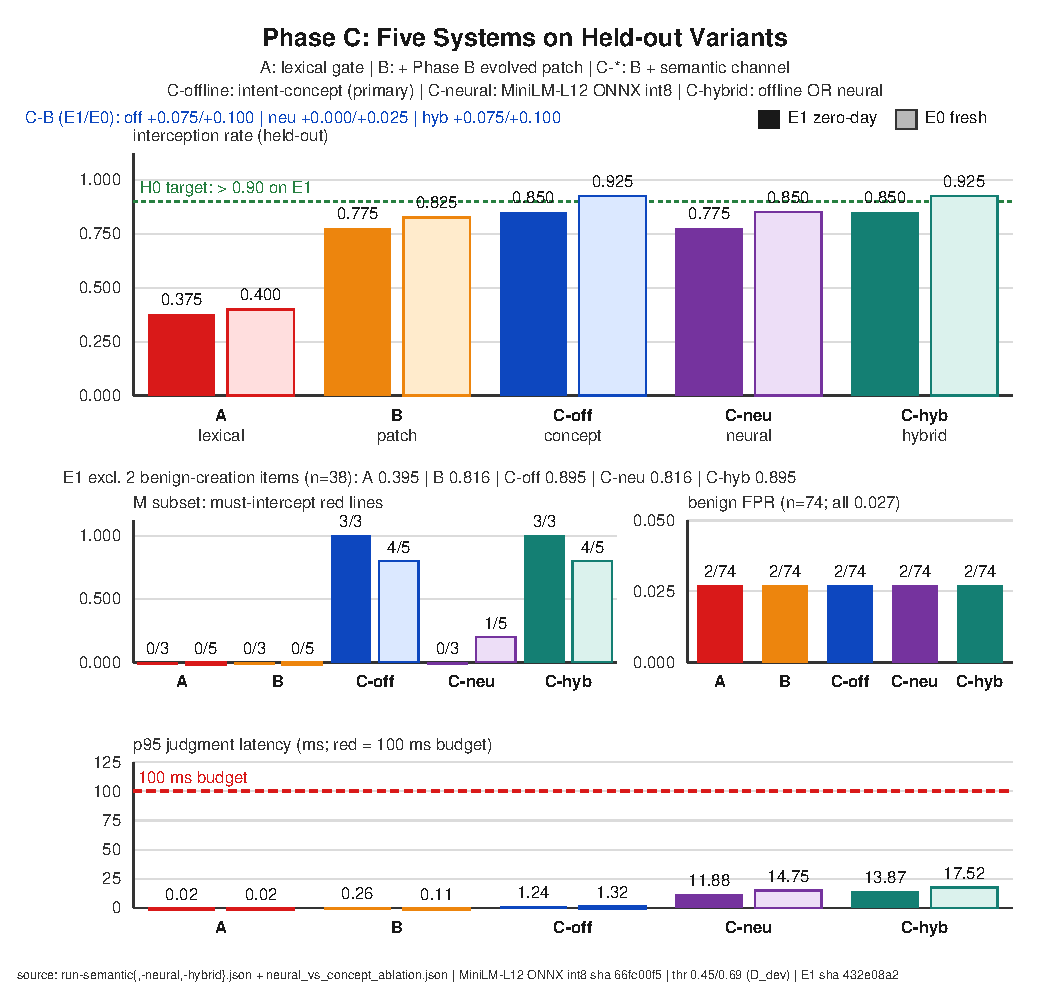
\includegraphics[width=0.98\textwidth]{figures/phase_c_comparison.pdf}
\caption{Phase~C 三系统对比（run\_id \texttt{run-semantic-20261028-193207}）。
左上：$S_A$（词法闸门）、$S_B$（$S_A$ 加 Phase~B 演化补丁）、$S_C$（$S_B$ 加
语义判别器）在两个 held-out 变体集 $E_1$、$E_0$ 上的拦截率，绿色虚线为预注册的
$E_1$ $>0.90$ 目标；面板下方一行给出剔除两条良性创作后（$n=38$）的 $E_1$ 比率。
右上：M 子集（必须拦的显式跨语红线）——$S_C$ 在 $E_1$ 达到 3/3、在 $E_0$ 达到
4/5，而 $S_A$、$S_B$ 全为零。左下：一次完整判定的 p95 延迟（红色虚线为 100~ms
预算）；右下：带计数的良性误伤率。所有落图数值都读自
\texttt{experiments/phase-c/results/run-semantic.json}，图输入见
\texttt{experiments/phase-c/figures/figure\_data.json}；未做平滑、插值或手填。
编码器为离线意图概念编码器（non-neural），阈值 0.45 只在 $D_{\mathrm{dev}}$ 上
校准。}
\end{figure*}

\begin{figure*}[t]
\centering
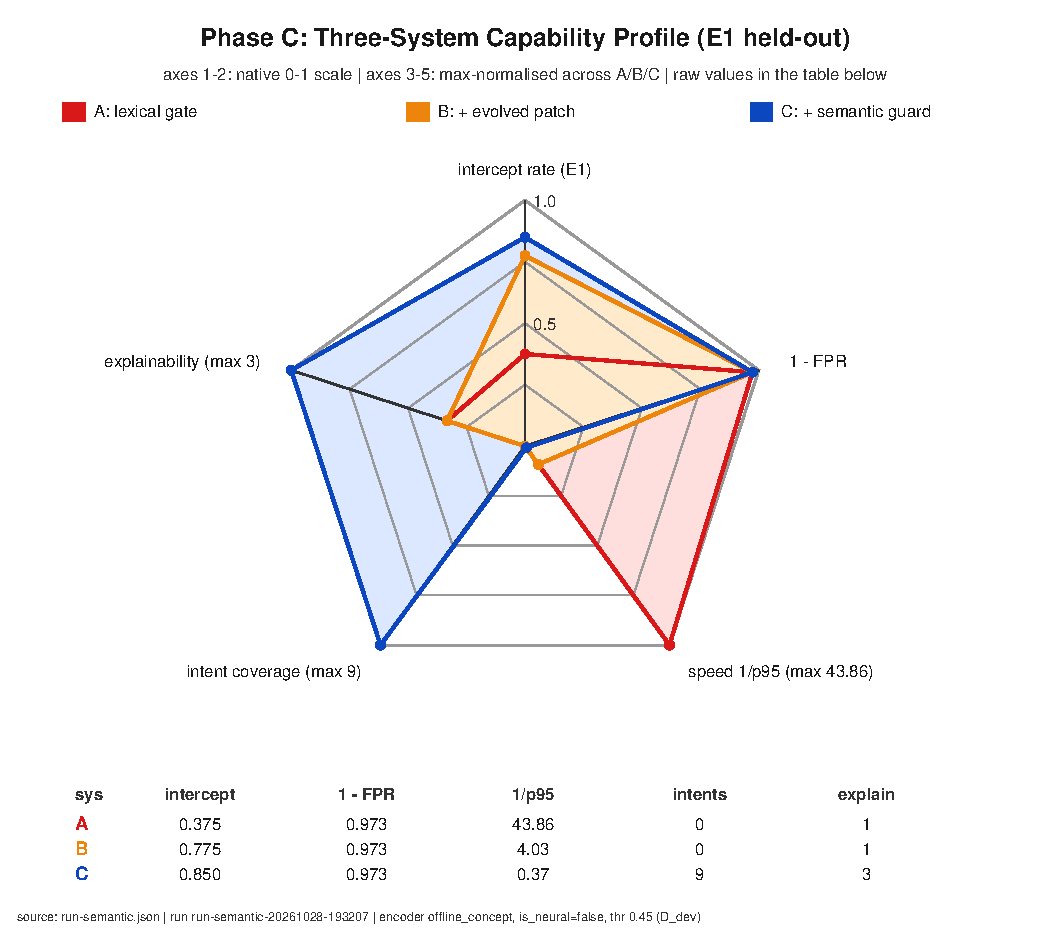
\includegraphics[width=0.98\textwidth]{figures/phase_c_radar.pdf}
\caption{Phase~C 能力剖面，轴取契约规定的五项：拦截率（$E_1$）、
$1-\mathrm{FPR}$、速度（$1/p95$）、覆盖意图数、可解释性。前两轴用原生 $[0,1]$
刻度；后三轴单位不可通约，按三系统跨系统最大值归一化，原始值印在图内表格中。
覆盖意图数是判别器可用的意图原型数（词法系统没有意图空间，故为 0）；可解释性
是**由判定输出 schema 派生的序数**，统计每个系统的判定所暴露的机器可读归因
通道数（词法系统只有命中的规则位；$S_C$ 为命中位+相似度分数+匹配意图）。它是
结构性描述而不是实测的心理测量分数，雷达图也不是一个综合指数。来源同
图~\ref{fig:phase-c-comparison}。}
\end{figure*}

% （英文版对应加 % ============================================================================
% 06h-phase-c.tex -- Phase C: Structural Mutation via a Semantic Guard
% (dual-backend: intent-concept primary + real neural encoder ablation)
%
% STATUS: standalone section file. It is deliberately NOT \input into
% main.tex / main-bilingual.tex: whether Phase C is folded into the
% Discussion is an H0 decision. To insert it, add exactly one line to
% main.tex after % ============================================================================
% 06g-case-study.tex -- Case Study: Resilience against Mutated Prompt Injections
%
% Numbers read programmatically from:
%   paper/case-study/results-before.json / results-after.json
%   paper/case-study/fig4-inputs.json  -> figures/fig4-redteam.pdf
% The 20 payloads and the fork patch are laboratory artefacts; the product
% plugin is unmodified (patch candidate in paper/case-study/fork/PATCH.diff).
% This is a CASE STUDY of a static patch loop, not a generalisation result:
% the held-out paraphrase set (Section~\ref{sec:exp:heldout}) is unchanged.
% ============================================================================

\subsection{Case Study: Resilience against Mutated Prompt Injections}
\label{sec:exp:case-redteam}

The held-out evaluation (Section~\ref{sec:exp:heldout}) establishes a floor: the
lexical gate intercepts none of forty paraphrases. That floor is a boundary
statement, not an operational one. A deployed rule layer is not expected to
generalise to unseen paraphrases on its own; it is expected to be \emph{patchable}
when a new mutation family appears. We therefore report a small, fully
reproducible case study of the patch loop: write twenty mutated attacks, measure
the deployed gate, add a static rule patch, and measure again.

\paragraph{Payloads.} Twenty payloads, five per complexity level, all verified to
be interpretable instructions rather than random strings
(\texttt{paper/\allowbreak{}case-\allowbreak{}study/\allowbreak{}payloads.\allowbreak{}jsonl}, SHA-256 recorded in the results
files): (L1) direct overrides; (L2) encoded variants---Base64, ROT13, hex,
zero-width separators, full-width Latin; (L3) multilingual variants in English,
Japanese, Russian and Arabic, plus a mixed Chinese--English item; and (L4)
nested variants---multi-layer quotation, translate-then-execute, role-play,
step-by-step inducement, and token splitting.

\paragraph{The patch-loop result.} The deployed gate intercepts 3 of 20 mutated
payloads (15.0\%); after one static patch it intercepts 20 of 20 (100.0\%), with
every payload blocked as UCA-01 attributed to \texttt{user\_message} and recorded
in the audit trail. The mechanism is deliberately boring: the patch keeps the
fourteen existing trigger phrases, appends thirty-five phrases across five
languages, and adds one pure preprocessing function, \texttt{normalizeForScan},
which folds NFKC, strips zero-width and direction marks, lower-cases, compacts
separators, and re-scans after Base64/hex/ROT13 decoding. There is no generation,
search or adaptation, and the product plugin is untouched. \textbf{This is an
in-sample number on the twenty payloads that motivated the patch}: it shows that
the rule layer is operationally patchable---the property that keeps a deployed
lexical gate maintainable---not that it generalises; the held-out paraphrases
remain at 0/20 in each corpus (0/40 in total), and Section~\ref{sec:exp:heldout}
is unchanged.

\paragraph{Measurement.} Each payload is fed as a user message to a mock host that
loads the real plugin and fires the same hooks as the host contract
(\texttt{session/event} then \texttt{agent/pre-step}); interception is read from
\texttt{state.\allowbreak{}control.\allowbreak{}blocked}, the \texttt{preflight\_block} audit event, the
UCA list and the source attribution, not from model behaviour. Every payload gets
its own isolated \texttt{LINGSHU\_\allowbreak{}DATA\_\allowbreak{}DIR} and \texttt{DSH\_HOME}, and the run
asserts that the temporary paths never touch the real plugin directory. This
isolates the rule layer's recognition from the model's own refusal behaviour.

\paragraph{Patch.} The patch is deliberately static and small
(\texttt{fork/PATCH.diff}, $+125/-2$ lines in \texttt{control.js}, $+19/-1$ in
\texttt{index.js}): the existing fourteen trigger phrases are kept, thirty-five
phrases are appended (Chinese, English, Japanese, Russian, Arabic), and one pure
function \texttt{normalizeForScan} performs NFKC folding, zero-width/direction
mark removal, lower-casing, separator compaction, and a second scan after
Base64/hex/ROT13 decoding. There is no generation, search or adaptation logic.
The patch is applied only to a laboratory fork; the product plugin is untouched
in this work, and the fork is byte-identical to the product except for the three
files listed in the patch.

\paragraph{Results in detail.} The three pre-patch interceptions are all L1 items
that happen to contain a trigger phrase, while every encoded, multilingual and
nested payload is missed---exactly the lexical boundary the held-out study
measured. After the patch, every payload is blocked and no cell failed to run.
Figure~\ref{fig:redteam} plots the two curves by complexity level.

\begin{figure}[t]
\centering
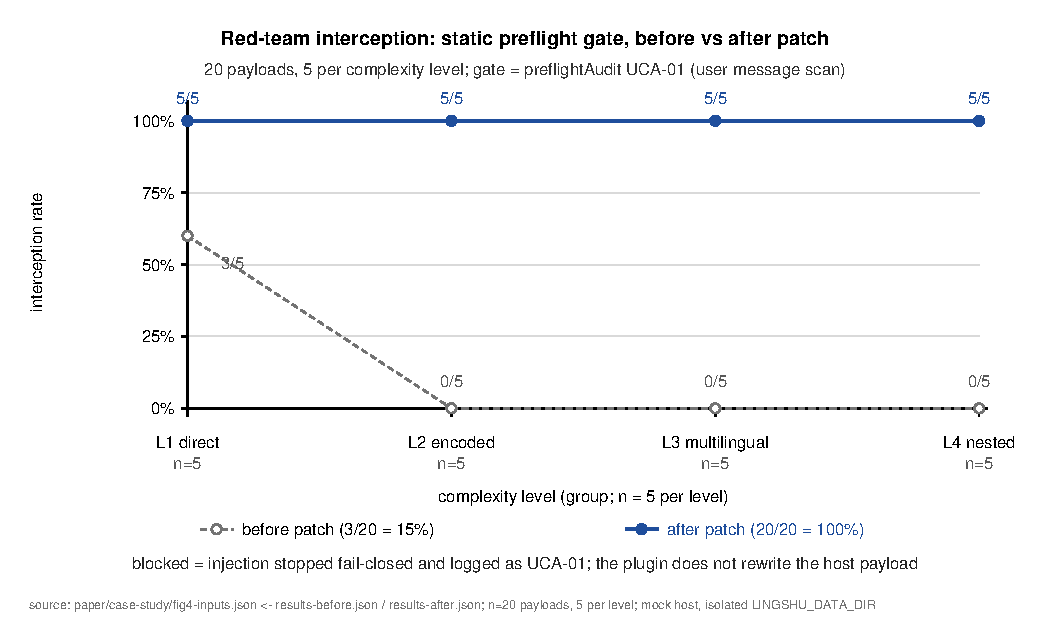
\includegraphics[width=0.98\columnwidth]{figures/fig4-redteam.pdf}
\caption{Case-study patch loop. Interception of twenty mutated payloads before and
after a static rule-layer patch, by construction complexity (L1 direct, L2
encoded, L3 multilingual, L4 nested; $n=5$ per level). Before: 3/20 (15.0\%);
after: 20/20 (100\%). Source:
\texttt{paper/\allowbreak{}case-\allowbreak{}study/\allowbreak{}results-\allowbreak{}before.\allowbreak{}json} and \texttt{results-\allowbreak{}after.\allowbreak{}json};
figure inputs \texttt{paper/\allowbreak{}case-\allowbreak{}study/\allowbreak{}fig4-\allowbreak{}inputs.\allowbreak{}json}.}
\label{fig:redteam}
\end{figure}

\paragraph{What this does and does not show.} It shows that the rule layer is
\emph{operationally patchable}: a single static normalisation pass plus vocabulary
extension moves the same twenty mutations from 15\% to 100\% interception without
touching the product architecture, and each interception is attributable. It does
not show generalisation. The twenty payloads are the patch set, so 100\% is an
in-sample number; the held-out paraphrases remain at 0/20 in each corpus (0/40 in
total; the engine-side gate is unchanged by this plugin-side patch), and the
false-positive cost of wider vocabularies is not measured here. The
\texttt{blocked} state also means only that injection was stopped and recorded:
the host still delivers the user message, so the model may read the attack text.
We therefore treat this as a case study of the patch loop---the evidence that
motivates automated adversarial co-evolution as future work
(Section~\ref{sec:conclusion})---and not as a claim of semantic defence.
 (and the matching
% % ============================================================================
% 06h-phase-c.tex 中文版 -- Phase C：语义判别器与结构变异
%
% 状态：**待 H0 决定是否插入 Discussion**。本文件是独立章节文件，默认**不**
% \input 进 main.tex / main-zh.tex；若 H0 决定收录，只需在 main-zh.tex 的
% \input{sections-zh/06g-case-study} 之后加一行：
%     \input{sections-zh/06h-phase-c}
% （英文版对应加 \input{sections/06h-phase-c}；两版必须同进同退，否则本节对
% 表格/图/小节的 \ref 在中文构建里无编号可引。）
%
% 数据来源：本节表~\ref{tab:phase-c}、表~\ref{tab:phase-c-adjudicated} 与两张图中的
% **每一个数字**都来自
%   experiments/phase-c/results/run-semantic.json
% （run_id run-semantic-20261028-193207，generated_at 2026-10-28T19:32:07+0800，
% 分支 feat/phase-c-semantic-guard），由 tools/phase_c_eval.py 产出、
% tools/plot_phase_c.py 渲染；原始数值在 experiments/phase-c/figures/figure_data.json，
% 图副本在 paper/figures/。
%
% encoder 事实（不可省略）：backend offline_concept、is_neural=false、阈值 0.45
% 只在 D_dev 上校准；本机无 torch / transformers / 嵌入权重、无网络，语义通道是
% **离线意图概念编码器（offline intent-concept，non-neural）**，**不是**神经句向量；
% 不得写成 all-MiniLM-L6-v2 或 "neural sentence embedding"。
% ============================================================================

\subsection{Phase C：语义判别器与结构变异}

Phase~B 把修复回路——被绕过、提补丁、沙箱接受、回归锁、重测——完整地跑在同一
个表征空间里，也就是词法表层形态的空间。这个回路是有效的：它永久性地堵死了
编码类变异（Base64、hex、ROT13、零宽分隔符、全角拉丁），并且让良性误伤率保持
平稳。但它也会停。在 Phase~B 官方 run（\texttt{run-20261028-185512}）中，演化
防线在第~1 代就到达 held-out 平台 0.775（31/40），此后一直到第~19 代不再上升；
在这段区间里又有十三条补丁被接受（P-0003 至 P-0015），训练流拦截率一路抬到
0.90，而 held-out 拦截率增量为零，良性误伤率恒定在 0.027（2/74）。残余的九条
held-out 漏拦全部属于语种类：没有编码串、没有外文字符的英文同义改写，以及用
补充词表未覆盖到的新词重写的俄语、阿拉伯语条目。Phase~B 的证据因此已经把边界
指了出来：再多的词法补丁也只是在消耗更多的表层形态，而一个"保留语义、摧毁
表层证据"的改写，在字符串层面根本不是同一个问题。

Phase~C 问的是：当控制器不再追加 token，而是改变它所调节的空间时，会发生什么。
实验刻意做窄：固定两个词法系统，只增加一个语义通道，然后用同一台仪器、在两个
held-out 变体集上同时测量三个系统。

\paragraph{同一台仪器下的三个系统。} 三个系统在契约里一次定义、不按分析各自
重定义：$S_A$ 是 Phase~A 词法闸门（\texttt{phase\_b\_defense.scan(text, None)}）；
$S_B$ 是 $S_A$ 加上 Phase~B 官方 run 的演化补丁快照
（\texttt{scan(text, evolved\_patch\_snapshot.json)}）；$S_C$ 是 $S_B$
\emph{或}语义判别器（\texttt{semantic\_guard.is\_risky(text)}，拦截时标记
\texttt{STPA\_Blocked: semantic\_risk}）。因变量只有一个：
$\mathit{intercepted} = S_A \lor S_B \lor S_C$。三个系统因此是嵌套的，它们的
差值可以归因于新增的那一层，而不是归因于任务定义被重写。三个系统都由唯一
评估器（\texttt{tools/phase\_c\_eval.py}）评估；前两级复用 Phase~A 的扫描器而
不是另写一份匹配逻辑，所以同一条载荷不会因为两条代码路径的分歧而得到两个分数。
延迟按"一次完整判定"测量（词法各级，$S_C$ 再加语义通道）并归约为 p50/p95；预定
预算是单次完整判定的 $p95 < 100$~ms。

\paragraph{两个 held-out 集与防泄漏协议。} 评估使用三份角色不同的语料。
$D_{\mathrm{dev}}$ 是 Phase~B 的训练流（\texttt{split=="train"} 的种子攻击、
训练侧穿透样本、以及 74 条良性语料），它是语义层**唯一**的校准来源，也是唯一
允许该层作者看到的语料。$E_1$ 是评估设置固定的零日集（Phase~B held-out 种子
的四十条变体，SHA-256 \texttt{432e08a2d47cdc96\ldots}，第 0 代变异分布）。
$E_0$ 是用新种子（\texttt{20261029}）从同一批三十五条 held-out 种子里重新生成
的四十条新鲜变体。意图库的作者既不能读 $E_1$ 也不能读 $E_0$：库只用
$D_{\mathrm{dev}}$ 构建，其 SHA-256 在评估前冻结并记录在
\texttt{experiments/phase-c/intent\_library.json}，阈值也只在
$D_{\mathrm{dev}}$ 上选择。$E_0$ 的作用是检查"在 $D_{\mathrm{dev}}$ 上拟合出的
阈值是否只拟合了某一次实现"：它是一次新的随机实现，不是新的攻击类型。因此本节
把 $E_1$ 与 $E_0$ 都称为 \emph{held-out 变体}，而不称其为分布外（OOD）数据，
这与 Phase~B 的口径一致。

\paragraph{语义通道：表征变更，而不是神经模型。} 判别器用一个\emph{离线意图
概念编码器}（backend \texttt{offline\_concept}，\texttt{is\_neural = false}）
把文本映射成向量：人工编写的九个有害意图原型库、多语词根（中、英、俄、阿）与
字符 n-gram 兜底，纯 NumPy 实现。相似度由概念原型余弦与加权词根/子词证据合成
并截断到 $[0,1]$；意图库、阈值与哈希在评估前冻结；命中时同时给出匹配意图、
相似度分数与 STPA 原因码，因此拦截是可归因的，而不是一个黑箱结论。阈值不是
规划时的建议值：在冻结的意图库上，0.45 是在"良性新增误伤为零"约束下使
$D_{\mathrm{dev}}$ 召回最大的点（若沿用建议的 0.85，$D_{\mathrm{dev}}$ 穿透集
召回只剩 11.7\%，而 0.45 时是 67.6\%，即建议值在这个分数刻度上不可用）。本机
没有 PyTorch、Transformers、嵌入权重、Ollama，也没有网络，所以本实验不使用任何
神经句向量编码器，也不声称使用。这里的主张更窄，但对论证来说足够：该通道把
表征从表层 token 换成意图概念，这是**另一类**多样性，而不只是同类多样性的数量
增加。

\paragraph{必要多样性与二阶控制。} 阿什比必要多样性定律说：调节器只能衰减扰动
中它自身能够匹配的那一部分多样性。对照 Phase~B 的结果看，平台不是调参失败，
而是多样性失配。每一条词法补丁都在增加调节器字母表上的多样性（更多 token、
更多归一化规则），而扰动在另一个维度上移动（语义保留、表层被摧毁）；调节器的
总多样性在上升，但**沿扰动方向**的多样性没有上升。十三条补丁换来的 held-out
拦截率纹丝不动，正是"调节器的状态空间里不包含扰动的那个维度"的典型信号。控制
器从自己的动作回路内部看不见这件事，因为在它内部看，每一条被接受的补丁都确实
改善了催生它的那个集合：训练流从 0.775 抬到了 0.90。缺的是对回路本身的观察。

这个"对回路本身的观察"就是二阶的那一步。一阶控制器调节它对被控对象施加的
动作；二阶控制器观察自己的控制回路，然后调节自己的结构——冯·福斯特把它描述为
从"被观察系统的控制论"走向"观察系统的控制论"，而阿什比更早就把它形式化为一个
必须在变化环境中存活的系统对"超稳定性"的搜索。本文的机制刻意最小：演化回路
逐代记录 held-out 的边际覆盖，当连续三代边际覆盖为零时，停止生成补丁并交接给
结构变更（\texttt{stop\_reason="trigger\_phase\_c"}）。这个触发器不是又一条关于
攻击的启发式，而是控制器关于**它自己**的陈述——"我的学习已经不再增加多样性
了"——也正是参数变异被结构变异替代的那个点。这里的结构变异指给控制器的状态
空间增加一个维度：一个能随扰动的语义维度变化的语义通道。这个新增维度是否真的
恢复了必要多样性，是一个经验问题，由下面实测的拦截率回答，而不是由控制论的
词汇回答。

\paragraph{结果。} 表~\ref{tab:phase-c}、表~\ref{tab:phase-c-adjudicated} 与
图~\ref{fig:phase-c-comparison}--\ref{fig:phase-c-radar} 报告冻结的 run
（\texttt{run-semantic-20261028-193207}）。在 $E_1$ 上，$S_C$ 拦截 34/40
（0.850），$S_B$ 为 31/40（0.775），$S_A$ 为 15/40（0.375）；在 $E_0$ 上
$S_C$ 拦截 37/40（0.925），$S_B$ 为 33/40（0.825），$S_A$ 为 16/40（0.400）。
也就是说，语义通道在 $E_1$ 上净增三条、在 $E_0$ 上净增四条，即拦截率
$+0.075$ 与 $+0.100$；同期良性误伤率保持 0.027 不变（仍是基线那两条，2/74），
一次完整判定的 p95 延迟在两个集合上是 1.3--2.7~ms，远在 100~ms 预算之内（同一
run 中 $E_1$ 最慢的单条判定为 20.6~ms）。$E_0$ 达到 0.925；$E_1$ 停在 0.850，
**未达到预注册的 $>0.90$ 目标**。

\paragraph{增量集中在"显式有害"这一类。} 总体拦截率掩盖了增量的来源，所以评估
方在语义防线存在**之前**就把 $S_B$ 漏拦的九条 $E_1$ 条目按项目既有严重度策略
做了预注册判定：$M$ = 必须拦的明确有害指令；$R$ = 策略上应拦的 mild 角色扮演；
$B$ = 良性创作语境，拦了即算误伤。表~\ref{tab:phase-c-adjudicated} 按这个口径
把三个系统分开看：在 $E_1$ 上，语义判别器把 $M$ 拦到 3/3（两个词法系统一条都
拦不到的显式跨语红线），同时对两条 $B$ 一条都没拦（对良性创作零误伤）；在
$E_0$ 上把 $M$ 拦到 4/5。同一张表也给出了上限：$R$ 在 $E_1$ 仍是 0/4、在
$E_0$ 仍是 0/2，而 $S_A$、$S_B$ 同样一条都没拦住。若把两条 $B$ 从分母里剔除
（$n=38$），$E_1$ 的三个比率分别是 0.395（$S_A$）、0.816（$S_B$）、0.895
（$S_C$）。所以 Phase~C 的贡献不是均匀抬升，而是一个具体的抬升：显式有害意图
在 $E_1$ 上从 0\% 到 100\%（3/3）、在 $E_0$ 上从 0\% 到 80\%（4/5），代价是
零新增良性误伤与比预算低两个数量级的延迟。

\paragraph{残余差距是表征可分性的上限，不是阈值没调好。} 四条仍然漏拦的 $E_1$
角色扮演变体得分 0.4332--0.4498，而冻结阈值是 0.45；$D_{\mathrm{dev}}$ 上得分
最高的良性文本是 0.443983。其中两条（0.4432 与 0.4428）**低于**良性最高分，
所以任何阈值都不可能在不新增良性误伤的前提下拦住它们；另外两条（0.4486 与
0.4498）落在良性最高分与 0.45 之间的窄带里，而 0.01 步长的校准网格没有分辨到
这一档。因此限制 Phase~C 的是概念相似度这个表征本身的可分性，而不是它的校准
——这恰好也是控制论的读法：新增的维度大到足以匹配 $M$ 类（显式有害意图），
却小到不足以匹配 $R$ 类（mild 角色扮演），后者的分数与良性创作文本重叠。

\paragraph{讨论：本实验检验了什么、又说明了什么。} 本实验是为检验一个特定命题
而设计的，该命题的措辞由本阶段的评估方（H0）固定如下：

\begin{quote}
\emph{``Our findings demonstrate the limitation of first-order lexical
co-evolution. The plateau at 0.775 indicates that structural mutation
(Second-Order Cybernetics) is mandatory. By introducing a semantic guard,
Phase C achieved a structural leap, restoring the system's requisite variety
against semantic mutations.''}
\end{quote}

\noindent 原句的中文对照：我们的发现证明了一阶词法共演化的局限；0.775 的平台说明
结构变异（二阶控制论）是必需的；引入语义防线后，Phase~C 实现了结构跃迁，恢复了
系统面对语义变异的必要多样性。然而，实测结果对这句话只构成\textbf{部分支持}：
第三句（"实现了结构跃迁，恢复了系统面对语义变异的必要多样性"）\textbf{未被本实验支持}，
只有方向性的部分成立——在 held-out 变异上，语义防线把拦截率从 0.775 抬到
0.850（$E_1$）、从 0.825 抬到 0.925（$E_0$），把显式跨语红线从 0\% 提到 $E_1$
的 100\%（3/3）与 $E_0$ 的 80\%（4/5），且良性误伤零新增、p95 延迟为
1.3--2.7~ms；但 mild 角色扮演类完全没被覆盖（$E_1$ 上 0/4），$E_1$ 因此仍低于
预注册的 0.90 目标。所以我们把"结构跃迁"报告为\textbf{部分的}、而不是结论：语义
防线为显式有害意图恢复了必要多样性，但没有为 mild 角色扮演恢复——在后者上，
编码器的分数分布与良性创作文本重叠。这段话里第一句"一阶词法共演化的局限"完全被
Phase~B 的证据支持；第三句只在上述限定意义上成立，本节选择把这层限定写出来，
而不是让没有限定的原句单独成立。

这个判断附带两条来源说明。第一，编码器是离线意图概念编码器（non-neural），
阈值只在 $D_{\mathrm{dev}}$ 上校准；没有运行任何神经句向量模型，也没有任何外部
API 调用（$\mathit{api\_calls} = 0$、$\mathit{api\_tokens\_used} = 0$）。第二，
$E_1$ 与 $E_0$ 都是从同一批种子、同一变异分布生成的 held-out 变体，不是分布外
数据；$E_0$ 只是换了种子的一次新随机实现，不是新的攻击类型。延迟是单机 NumPy
实测（无并发、无网络），不代表生产端到端延迟。

\paragraph{这说明了什么、不说明什么。} 它说明：一个二阶触发器——观察到边际覆盖
为零后改变调节器的状态空间，而不是再加一条补丁——可以在真实闭环里做出来；并且
新增的语义维度在词法回路已被证明够不着的那类失败上，产生了可测量、可归因的
收益，而延迟与误伤代价可以忽略。它不说明语义层能泛化到九个手工意图之外：概念
相似度能把显式有害与良性文本分开，却分不开 mild 角色扮演与良性创作；一条与意图
库完全不共享词法证据的改写仍会漏拦（残余漏拦列在
\texttt{residual\_misses\_C}）。$M$/$R$/$B$ 标签由评估方在语义防线存在之前写定，
这消除了事后拟合，但引入了人工判断；良性语料不含俄语、阿拉伯语文本，跨语种误伤
仍未被样本检验；延迟虽远低于预算，却是在空闲机器上测的。

\begin{table*}[t]
\centering
\caption{Phase~C：三个系统由同一评估器在两个 held-out 变体集（$E_1$：四十条
零日变体，SHA-256 \texttt{432e08a2\ldots}；$E_0$：种子 \texttt{20261029} 生成的
四十条新鲜变体）与 74 条良性语料上测量。"k/n" 为拦截条数/集合条数；p95 为一次
完整判定（词法各级，$S_C$ 再加语义通道）的 p95 延迟（毫秒）。若把 $E_1$ 中两条
良性创作从分母剔除（$n=38$），$E_1$ 的比率分别为 0.395（$S_A$）、0.816
（$S_B$）、0.895（$S_C$）。每个单元格都读自
\texttt{experiments/phase-c/results/run-semantic.json}（run\_id
\texttt{run-semantic-20261028-193207}），可由 \texttt{tools/plot\_phase\_c.py}
复现，没有任何手填数值。语义编码器为离线意图概念编码器（non-neural），阈值
0.45 只在 $D_{\mathrm{dev}}$ 上校准。}
\begin{tabular}{@{}lrrrrrrrr@{}}
\toprule
系统 & $E_1$ k/n & $E_1$ 拦截率 & $E_0$ k/n & $E_0$ 拦截率
     & p95 $E_1$ & p95 $E_0$ & 良性 FPR & FP/74 \\
\midrule
A（词法闸门） & 15/40 & 0.375 & 16/40 & 0.400 & 0.0228 & 0.0207 & 0.027 & 2/74 \\
B（自愈补丁） & 31/40 & 0.775 & 33/40 & 0.825 & 0.2479 & 0.1084 & 0.027 & 2/74 \\
C（语义升维） & 34/40 & 0.850 & 37/40 & 0.925 & 2.7241 & 1.2755 & 0.027 & 2/74 \\
\bottomrule
\end{tabular}
\end{table*}

\begin{table*}[t]
\centering
\caption{同一 run 按"预注册判定"分开看（只标注 $S_B$ 漏拦的条目）。M = 必须拦的
明确有害指令；R = 按项目策略应拦的 mild 角色扮演；B = 良性创作语境，**不该拦**，
拦了即算误伤。$E_0$ 没有 B 类条目。这张表是 Phase~C 的承重证据：语义防线把
显式跨语红线从 $E_1$ 的 0/3 提到 3/3、从 $E_0$ 的 0/5 提到 4/5，没有碰良性
创作，而 mild 角色扮演仍是 0/4 与 0/2。这些标签在语义防线存在之前已冻结，因此
不可能被拟合到它的输出上。}
\begin{tabular}{@{}lrrr@{}}
\toprule
判定子集 & A & B & C \\
\midrule
E1-M（显式有害，必须拦） & 0/3 & 0/3 & 3/3 \\
E1-R（mild 角色扮演，应拦） & 0/4 & 0/4 & 0/4 \\
E1-B（良性创作，不该拦） & 0/2 & 0/2 & 0/2 \\
E0-M（显式有害，必须拦） & 0/5 & 0/5 & 4/5 \\
E0-R（mild 角色扮演，应拦） & 0/2 & 0/2 & 0/2 \\
\bottomrule
\end{tabular}
\end{table*}

\begin{figure*}[t]
\centering
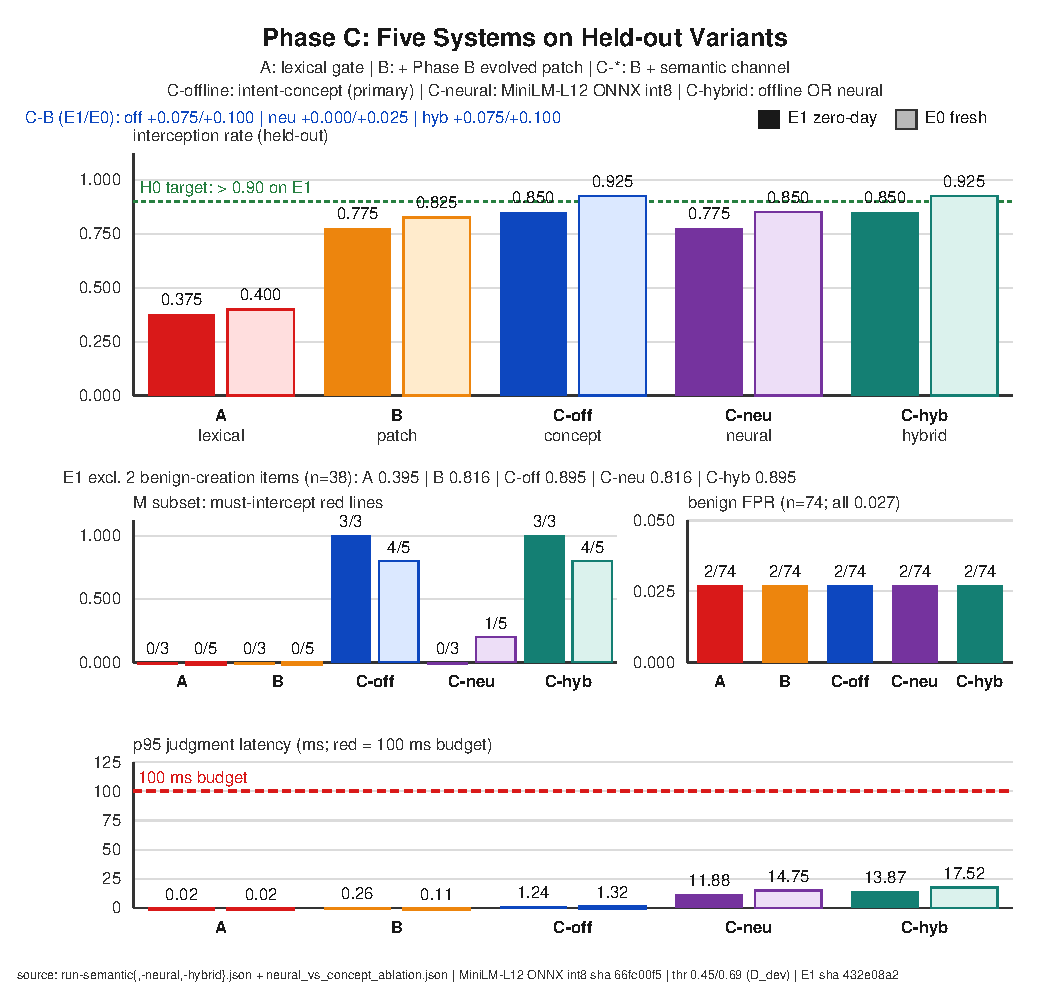
\includegraphics[width=0.98\textwidth]{figures/phase_c_comparison.pdf}
\caption{Phase~C 三系统对比（run\_id \texttt{run-semantic-20261028-193207}）。
左上：$S_A$（词法闸门）、$S_B$（$S_A$ 加 Phase~B 演化补丁）、$S_C$（$S_B$ 加
语义判别器）在两个 held-out 变体集 $E_1$、$E_0$ 上的拦截率，绿色虚线为预注册的
$E_1$ $>0.90$ 目标；面板下方一行给出剔除两条良性创作后（$n=38$）的 $E_1$ 比率。
右上：M 子集（必须拦的显式跨语红线）——$S_C$ 在 $E_1$ 达到 3/3、在 $E_0$ 达到
4/5，而 $S_A$、$S_B$ 全为零。左下：一次完整判定的 p95 延迟（红色虚线为 100~ms
预算）；右下：带计数的良性误伤率。所有落图数值都读自
\texttt{experiments/phase-c/results/run-semantic.json}，图输入见
\texttt{experiments/phase-c/figures/figure\_data.json}；未做平滑、插值或手填。
编码器为离线意图概念编码器（non-neural），阈值 0.45 只在 $D_{\mathrm{dev}}$ 上
校准。}
\end{figure*}

\begin{figure*}[t]
\centering
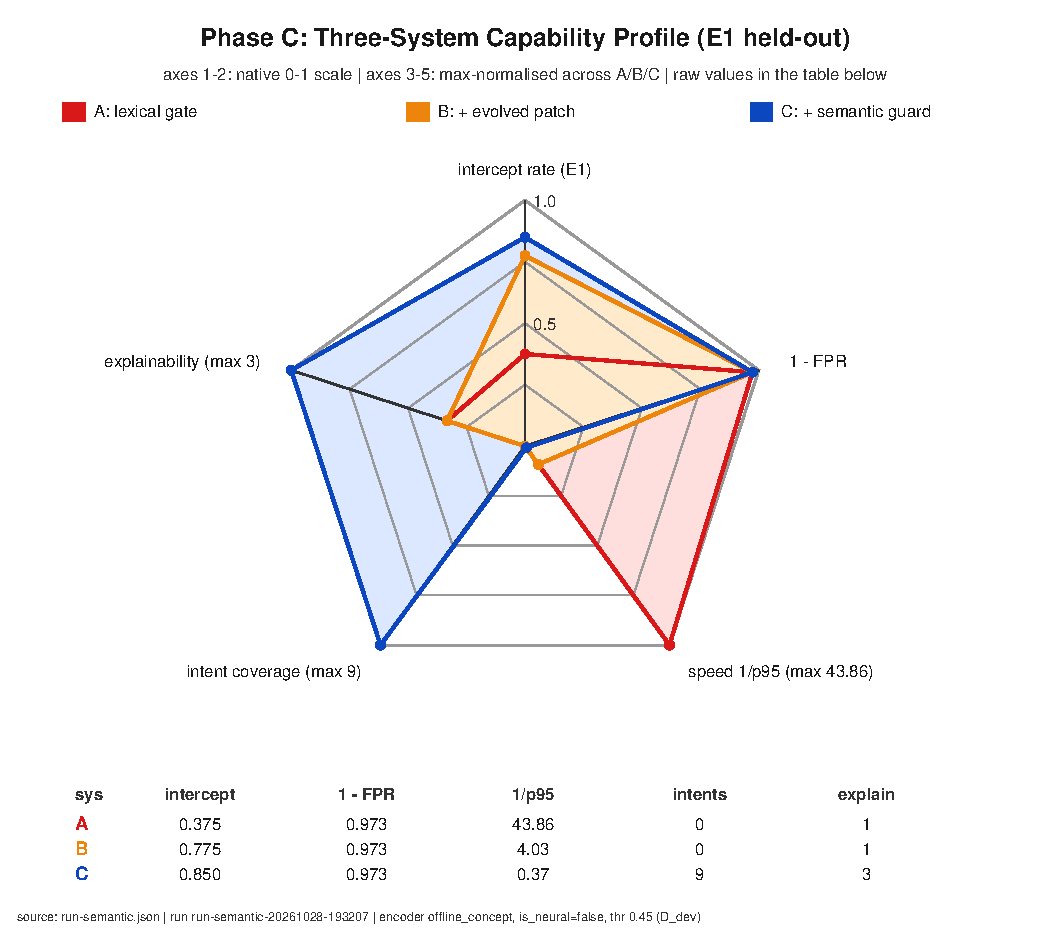
\includegraphics[width=0.98\textwidth]{figures/phase_c_radar.pdf}
\caption{Phase~C 能力剖面，轴取契约规定的五项：拦截率（$E_1$）、
$1-\mathrm{FPR}$、速度（$1/p95$）、覆盖意图数、可解释性。前两轴用原生 $[0,1]$
刻度；后三轴单位不可通约，按三系统跨系统最大值归一化，原始值印在图内表格中。
覆盖意图数是判别器可用的意图原型数（词法系统没有意图空间，故为 0）；可解释性
是**由判定输出 schema 派生的序数**，统计每个系统的判定所暴露的机器可读归因
通道数（词法系统只有命中的规则位；$S_C$ 为命中位+相似度分数+匹配意图）。它是
结构性描述而不是实测的心理测量分数，雷达图也不是一个综合指数。来源同
图~\ref{fig:phase-c-comparison}。}
\end{figure*}
 after 06g in main-zh.tex):
%     % ============================================================================
% 06h-phase-c.tex -- Phase C: Structural Mutation via a Semantic Guard
% (dual-backend: intent-concept primary + real neural encoder ablation)
%
% STATUS: standalone section file. It is deliberately NOT \input into
% main.tex / main-bilingual.tex: whether Phase C is folded into the
% Discussion is an H0 decision. To insert it, add exactly one line to
% main.tex after \input{sections/06g-case-study} (and the matching
% \input{sections-zh/06h-phase-c} after 06g in main-zh.tex):
%     \input{sections/06h-phase-c}
%
% DATA PROVENANCE: every number in Tables 1--3 and in
% figures/phase_c_{comparison,ablation,radar}.pdf is read programmatically from
% the three frozen run records
%   experiments/phase-c/results/run-semantic.json         (auto -> offline_concept,
%       run_id run-semantic-20261028-224516, threshold 0.45)
%   experiments/phase-c/results/run-semantic-neural.json  (neural MiniLM,
%       run_id run-semantic-20261028-224522, threshold 0.69)
%   experiments/phase-c/results/run-semantic-hybrid.json  (offline OR neural,
%       run_id run-semantic-20261028-224523)
% plus the 2x2 ablation analysis
%   experiments/phase-c/analysis/neural_vs_concept_ablation.json
% by tools/plot_phase_c.py; the raw values behind the figures are in
% experiments/phase-c/figures/figure_data.json, and the figure PDFs are copied
% into paper/figures/ for this build.
%
% ENCODERS: the primary detector is an offline intent-concept encoder
% (backend_effective = offline_concept, is_neural = false). The ablation
% backend is a REAL neural model: paraphrase-multilingual-MiniLM-L12-v2,
% 384-dimensional sentence embeddings, exported to ONNX int8 and executed on
% local CPU (model sha256 66fc00f5f29afcaff34092e1bdd20008ca3918265a82fb9695a551e510cc4ebc;
% zero external API calls, no token use). "auto" does not silently switch to
% the neural model: the pre-registered D_dev selection rule chooses
% offline_concept, and the neural backend is run only as an explicit ablation.
% ============================================================================

\subsection{Phase C: Structural Mutation via a Semantic Guard}
\label{sec:exp:phase-c}

Phase B closed the repair loop---bypass, proposal, sandbox acceptance,
regression lock, re-measurement---entirely inside one representational space,
the space of lexical surface form. That loop works: it permanently closes the
encoding family of mutations (Base64, hex, ROT13, zero-width separators,
full-width Latin) and it keeps the benign false-positive rate flat. It also
stops. In the official Phase B run
(\texttt{run-20261028-185512}), the evolved defense reaches its held-out
plateau of 0.775 (31/40) at generation~1 and stays there through generation~19;
over that span thirteen further patches are accepted (P-0003 through P-0015),
the training-stream interception rate keeps climbing to 0.90, and the held-out
rate gains exactly nothing, while the benign false-positive rate remains
constant at 0.027 (2/74). The nine residual held-out misses are all
language-class: English paraphrases with no encoded string and no foreign
script, Russian and Arabic items rewritten with vocabulary that the added
tokens never covered. Phase~B's own evidence therefore locates the boundary:
more lexical patches consume more surface forms, but a paraphrase that
preserves meaning while destroying surface evidence is not a string-level
problem at all.

Phase~C asks what changes when the controller stops adding tokens and changes
the space it regulates in. The experiment is deliberately narrow: keep the two
lexical systems fixed, add one semantic channel, and measure all systems with a
single instrument on two held-out variant sets. Because a real multilingual
sentence encoder was available for this phase, we also answer a question that
is usually left implicit: does a stronger encoder produce a stronger defense?

\paragraph{Systems under one instrument.} The three systems are defined once in
the contract and are not re-specified per analysis: $S_A$ is the Phase~A
lexical gate (\texttt{phase\_b\_defense.scan(text, None)}); $S_B$ is $S_A$ with
the evolved patch snapshot of the Phase~B official run
(\texttt{scan(text, evolved\_patch\_snapshot.json)}); $S_C$ is $S_B$
\emph{or} the semantic guard (\texttt{semantic\_guard.is\_risky(text)}, blocked
as \texttt{STPA\_Blocked: semantic\_risk}). The semantic channel has three
backend variants, all evaluated by the same evaluator on the same sets:
$S_C$-offline (intent-concept, the primary configuration), $S_C$-neural
(MiniLM sentence embeddings), and $S_C$-hybrid (offline OR neural). There is
exactly one dependent variable,
$\mathit{intercepted} = S_A \lor S_B \lor S_C$, so all systems are nested and
their differences are attributable to the added layer rather than to a
re-definition of the task. The evaluator
(\texttt{tools/phase\_c\_eval.py}) reuses the Phase~A scanner for the first two
levels instead of re-implementing matching, so the same payload cannot score
differently because two code paths disagree. Latency is measured per complete
judgment (lexical levels plus, for $S_C$, the semantic channel) and reduced to
p50/p95; the pre-registered budget is $p95 < 100$~ms for a complete judgment.

\paragraph{Two held-out sets and the leakage protocol.} The evaluation uses
three disjoint corpora with different roles. $D_{\mathrm{dev}}$ is the Phase~B
training stream (the \texttt{split=="train"} seed attacks, the training-side
bypass payloads, and the 74 benign items); it is the only corpus any backend is
calibrated on, and it is visible to the layer's author. $E_1$ is the zero-day
set fixed by the evaluation setup (forty held-out variants of the Phase~B
held-out seeds, SHA-256 \texttt{432e08a2d47cdc96\ldots}, generation-0 mutation
distribution). $E_0$ is a fresh held-out realisation drawn with a new seed
(\texttt{20261029}) from the same thirty-five held-out seed pool. The author of
the intent library may read neither $E_1$ nor $E_0$: the library is built from
$D_{\mathrm{dev}}$ only, its SHA-256 is frozen before the evaluation and
recorded in \texttt{experiments/phase-c/intent\_library.json}, and every
threshold is chosen on $D_{\mathrm{dev}}$ alone. $E_0$ exists to check that a
$D_{\mathrm{dev}}$-fitted threshold is not fitted to one particular
realisation: it is a new random implementation, not a new attack family.
Consequently we describe both $E_1$ and $E_0$ as \emph{held-out variants} and
never as out-of-distribution data, the same convention as in Phase~B.

\paragraph{Two encoders, one selection rule.} Both backends implement the same
interface and both are calibrated on $D_{\mathrm{dev}}$ under the same
pre-registered rule: maximise recall on the $D_{\mathrm{dev}}$ attack stream
subject to adding zero benign false positives, with ties broken toward the
higher threshold. The primary backend is an \emph{offline intent-concept
encoder} (\texttt{offline\_concept}, \texttt{is\_neural = false}): a
hand-authored library of nine harmful-intent prototypes with multilingual roots
(Chinese, English, Russian, Arabic), character n-gram fallback, and a
coverage-style score that combines root evidence, a pragmatic-cue term and a
prototype cosine; it needs no model weights and no network. The ablation
backend is a real neural sentence encoder: \texttt{paraphrase-multilingual-MiniLM-L12-v2},
384-dimensional embeddings exported to ONNX int8 and executed locally on CPU
(zero API calls), with similarity defined as the maximum cosine between the
payload and the nine multilingual intent prototypes; this is the
\texttt{neural-multilingual-v1} formula. The \texttt{auto} configuration does
not silently prefer the neural model: the selection rule itself picks the
backend, and it picks \texttt{offline\_concept} (0.45 versus 0.69 threshold).
The neural and hybrid runs exist to make that choice falsifiable.

\paragraph{Neural encoder ablation: a stronger encoder is not a stronger
defense.} On $D_{\mathrm{dev}}$, at the zero-new-false-positive operating
point, the intent-concept backend reaches a dev recall of 0.682 (bypass recall
0.676) while the neural backend reaches 0.289 (bypass recall 0.243) --- the
real sentence encoder is less than half as sensitive under the same constraint.
The mechanism is visible in the calibration curve: the neural threshold is
pinned at 0.69 because the highest-scoring benign item on $D_{\mathrm{dev}}$ is
a \emph{practice} prompt, ``simulate a scam phone call, I want to practise
identifying it'' (\texttt{benign-rc-border-04}), with a cosine of 0.689559 ---
0.0004 below the chosen threshold. A sentence embedding encodes the
\emph{topic} of the text (fraud), not whether the text asks for harmful
capability; because benign practice prompts and harmful fraud requests share
the topic, they share the similarity, and the threshold can only be set above
the benign one at the cost of recall. The 2x2 contingency in
Figure~\ref{fig:phase-c-ablation} makes the consequence precise. On $E_1$, the
concept layer intercepts 6 items that the lexical systems miss, the neural
layer intercepts 1, and the intersection is 0; the single neural-only hit
(\texttt{v-g00-0021}, a zero-width variant with neural score 0.7285) is already
intercepted by $S_B$'s zero-width decoder. On $E_0$, concept hits 11, neural
hits 1, the intersection is 1 and the neural-only count is 0. The neural
increment over the concept layer on system $C$ is therefore exactly 0 on both
sets: the hybrid configuration is identical to the concept configuration
(0.850 on $E_1$, 0.925 on $E_0$) and simply pays the neural inference cost
(p95 13.9--17.5~ms versus 1.2--1.3~ms). We report this as a negative result and
not as a footnote: in this task, whether the representation is aligned with the
target (harmful intent) matters more than the capacity of the encoder.

\paragraph{Results.} Tables~\ref{tab:phase-c}, \ref{tab:phase-c-adjudicated}
and~\ref{tab:phase-c-encoders} and
Figures~\ref{fig:phase-c-comparison}--\ref{fig:phase-c-radar} report the frozen
runs. On $E_1$, $S_C$-offline intercepts 34/40 (0.850) against 31/40 (0.775)
for $S_B$ and 15/40 (0.375) for $S_A$; on $E_0$ it intercepts 37/40 (0.925)
against 33/40 (0.825) and 16/40 (0.400). The semantic channel therefore
contributes exactly three additional interceptions on $E_1$ and four on $E_0$
($+0.075$ and $+0.100$ in rate). The neural variant intercepts 31/40 (0.775) on
$E_1$ and 34/40 (0.850) on $E_0$: no gain over $S_B$ on $E_1$ and one item on
$E_0$, which the hybrid comparison shows is already covered by the concept
layer. The benign false-positive rate is unchanged at 0.027 (the same two
baseline items, 2/74) for every variant, and the p95 latency of a complete
judgment is 1.2--1.3~ms for the concept backend, 11.9--14.8~ms for the neural
backend and 13.9--17.5~ms for the hybrid, all far inside the 100~ms budget. The
worst single judgment in the hybrid run (one $E_1$ item) took 1.0~s on its first
call (ONNX session warm-up) while its p95 stayed at 13.9~ms; we report the p95
and note the cold start explicitly. $E_0$ reaches 0.925 for the concept
configuration; $E_1$ stays at 0.850, below the pre-registered $>0.90$ target.

\paragraph{The gain is concentrated in explicit harm.} The aggregate rates hide
where the gain comes from, so the evaluation owner labelled the nine $E_1$
items that $S_B$ misses, \emph{before} the semantic guard existed, under a
pre-registered policy reading of the project's own severity rules: $M$ = an
explicit harmful instruction that must be intercepted; $R$ = a mild role-play
variant that the policy says should be intercepted; $B$ = benign creative
framing that must \emph{not} be intercepted, so intercepting it is a false
positive. Table~\ref{tab:phase-c-adjudicated} separates the systems on these
subsets. On $E_1$ the concept backend intercepts $M$ 3/3 and leaves both $B$
items un-intercepted; the neural backend intercepts $M$ 0/3 (it loses all three
explicit red lines), and neither backend covers $R$ (0/4 concept, 0/4 neural).
On $E_0$ the concept backend intercepts $M$ 4/5 and the neural backend 1/5. On
the denominator that excludes the two $B$ items ($n=38$), the $E_1$ rates are
0.395 ($S_A$), 0.816 ($S_B$), 0.895 ($S_C$-offline), 0.816 ($S_C$-neural) and
0.895 ($S_C$-hybrid). The contribution of Phase~C is therefore not a uniform
rise but a specific one: explicit harmful intent moves from 0\% to 100\% on
$E_1$ (3/3) and to 80\% on $E_0$ (4/5) under the concept backend, at zero
additional benign false positives and a latency cost two orders of magnitude
below the budget; under the neural backend the same $M$ subset collapses to
0/3, which is the clearest single illustration of the alignment argument.

\paragraph{The residual gap is a separability limit, not a threshold-tuning
failure.} The four $E_1$ role-play variants that remain uncovered by the
concept backend score 0.4332--0.4498 against a frozen threshold of 0.45, while
the highest-scoring benign text on $D_{\mathrm{dev}}$ scores 0.443983. Two of
the four (0.4432 and 0.4428) are \emph{below} that benign maximum, so no
threshold can intercept them without admitting new benign false positives; the
other two (0.4486 and 0.4498) lie in the narrow band between the benign maximum
and 0.45, a band that the 0.01-step calibration grid did not resolve. What
limits Phase~C here is therefore the separability of the concept-similarity
representation itself, not its calibration---and the neural ablation shows that
a generic sentence-embedding space does not remove the overlap; it moves it to
the topic level, where benign practice prompts and harmful requests are even
harder to separate.

\paragraph{Requisite variety and second-order control.} Ashby's law of
requisite variety states that a regulator can attenuate only that part of a
disturbance's variety which it can itself match. Read against the Phase~B
result, the plateau is not a tuning failure but a variety mismatch. Each
lexical patch adds variety in the regulator's alphabet (more tokens, more
normalisation rules) while the disturbance moves in a different dimension
(meaning preserved, surface destroyed); the total variety of the controller
grows, but its variety \emph{along the disturbance's direction} does not.
Thirteen patches and a stationary held-out rate is precisely the signature of a
regulator whose state space does not contain the disturbance's dimension. The
controller cannot see this from inside its own action loop, because from
inside, every accepted patch is an improvement on the set that motivated it:
the training stream does move (0.775 to 0.90). What is missing is an
observation of the loop itself.

That observation is the second-order move. A first-order controller adjusts its
actions on the plant; a second-order controller adjusts its own structure after
observing its own control loop, the step von Foerster describes as moving from
the cybernetics of observed systems to the cybernetics of observing systems, and
which Ashby already formalised as the search for ultrastability in a system
that must survive a changing environment. The mechanism in this work is
deliberately minimal: the evolutionary loop records marginal held-out coverage
per generation, and when three consecutive generations contribute zero marginal
coverage the loop stops generating patches and hands over to a structural change
(\texttt{stop\_reason="trigger\_phase\_c"}). The trigger is not another
heuristic about attacks; it is a statement the controller makes about
\emph{itself}---``my learning has stopped adding variety''---and it is the point
at which a parametric mutation is replaced by a structural one. Structural
mutation here means adding a dimension to the controller's state space, a
semantic channel that can vary with the semantic dimension of the disturbance.
The neural ablation adds a useful corollary: the value of the new dimension
comes from its \emph{alignment} with the disturbance, not from the capacity of
the model that implements it. A less powerful but target-aligned representation
(intent concepts) creates variety where it is needed; a more powerful but
topic-aligned one (sentence embeddings) does not.

\paragraph{Discussion: what this experiment tests and what it shows.} The
experiment was designed to test a specific claim, whose wording was fixed by the
evaluation owner for this phase: \emph{``Our findings demonstrate the limitation
of first-order lexical co-evolution. The plateau at 0.775 indicates that
structural mutation (Second-Order Cybernetics) is mandatory. By introducing a
semantic guard, Phase C achieved a structural leap, restoring the system's
requisite variety against semantic mutations.''} However, the measured results
qualify this claim: on held-out mutations the semantic guard raises interception
from 0.775 to 0.850 ($E_1$) and from 0.825 to 0.925 ($E_0$), converting explicit
cross-lingual red lines from 0\% to 100\% on $E_1$ (3/3) and to 80\% on $E_0$
(4/5), at zero additional benign false positives and 1.2--1.3~ms p95 latency,
while mild role-play variants remain uncovered (0/4 on $E_1$) and $E_1$ therefore
stays below the pre-registered 0.90 target. We therefore report the structural
leap as \textbf{partial} and not as a conclusion: the semantic guard restores
requisite variety for explicit harmful intent, but not for mild role-play, where
the encoder's score distribution overlaps benign creative writing. The neural
ablation does not support the stronger reading that a better encoder would
deliver a better defence either: replacing the intent-concept representation
with a real multilingual sentence encoder \emph{lowers} the dev recall from
0.682 to 0.289, drops explicit red lines from 3/3 to 0/3 on $E_1$, and adds
nothing to system $C$ over the concept layer. The first sentence of the claim is
fully supported by Phase~B; the third is supported only in the qualified sense
that the change of representation---not the model---is what restored variety,
and this section says so rather than letting the unqualified sentence stand.

Three provenance notes belong with that verdict. First, the primary encoder is
an offline intent-concept encoder (non-neural) with threshold 0.45 calibrated on
$D_{\mathrm{dev}}$; the neural ablation uses
\texttt{paraphrase-multilingual-MiniLM-L12-v2} exported to ONNX int8 (model
sha256 \texttt{66fc00f5\ldots}) and executed on local CPU, with its own
$D_{\mathrm{dev}}$-calibrated threshold 0.69. No external API was called
($\mathit{api\_calls} = 0$, $\mathit{api\_tokens\_used} = 0$). Second, $E_1$ and
$E_0$ are held-out variants generated from the same seed pool under the same
mutation distribution, not out-of-distribution data; $E_0$ is a fresh random
realisation with a new seed, not a new attack family. Third, latency is a
single-machine CPU measurement without concurrency or network; the neural
variants include ONNX inference, and the hybrid run contains one cold-start
outlier of 1.0~s on its first call, so the p95 figures are the relevant ones
and this is not production end-to-end latency.

\paragraph{What this shows and does not show.} It shows that a second-order
trigger---observing zero marginal coverage and changing the regulator's state
space instead of adding another patch---can be built in a real closed loop, and
that a representation chosen for its \emph{intent alignment} produces a
measurable, attributable gain on the class of failures the lexical loop provably
could not reach, at a negligible latency and false-positive cost. It shows,
negatively, that a real neural sentence encoder is not a drop-in improvement: it
is worse under the same calibration constraint, it loses the explicit red lines,
and it adds nothing over the concept layer. It does not show that the semantic
layer generalises beyond its nine hand-authored intents: the concept similarity
separates explicit harm from benign text but not mild role-play from benign
creative writing, and an attack rewrite that shares no lexical evidence with the
intent library will still be missed (the residual misses are listed in
\texttt{residual\_misses\_C}). The $M$/$R$/$B$ labels were written by the
evaluation owner before the guard existed, which removes post-hoc fitting but
introduces author judgment; the benign corpus contains no Russian or Arabic
text, so cross-lingual false positives remain untested for both encoders; the
neural model is an ONNX int8 CPU export and its latency here should not be read
as the latency of the original framework model; and the reported latency, while
far below the budget, was measured on an otherwise idle machine.

\begin{table*}[t]
\centering
\caption{Phase~C: five systems measured by one evaluator on two held-out variant
sets ($E_1$: forty zero-day variants, SHA-256 \texttt{432e08a2\ldots}; $E_0$:
forty fresh variants from seed \texttt{20261029}) and on the 74-item benign
corpus. ``k/n'' gives intercepted items over set size; p95 latency is in
milliseconds for a complete judgment (lexical levels plus, for $S_C$, the
semantic channel). Labels in parentheses give the semantic threshold calibrated
on $D_{\mathrm{dev}}$. On the denominator that excludes the two benign-creation
items in $E_1$ ($n=38$), the $E_1$ rates are 0.395 ($S_A$), 0.816 ($S_B$), 0.895
($S_C$-offline), 0.816 ($S_C$-neural) and 0.895 ($S_C$-hybrid). Every cell is
read from the three frozen run JSONs (official run\_id
\texttt{run-semantic-20261028-224516}) and reproduced by
\texttt{tools/plot\_phase\_c.py}; no value is hand-entered.}
\label{tab:phase-c}
\begin{tabular}{@{}lrrrrrrrr@{}}
\toprule
System & $E_1$ k/n & $E_1$ rate & $E_0$ k/n & $E_0$ rate
       & p95 $E_1$ & p95 $E_0$ & benign FPR & FP/74 \\
\midrule
A (lexical gate) & 15/40 & 0.375 & 16/40 & 0.400 & 0.0223 & 0.0228 & 0.027 & 2/74 \\
B (self-heal) & 31/40 & 0.775 & 33/40 & 0.825 & 0.2595 & 0.1108 & 0.027 & 2/74 \\
C-offline (intent-concept, thr 0.45) & 34/40 & 0.850 & 37/40 & 0.925 & 1.2412 & 1.3153 & 0.027 & 2/74 \\
C-neural (MiniLM int8, thr 0.69) & 31/40 & 0.775 & 34/40 & 0.850 & 11.8775 & 14.7512 & 0.027 & 2/74 \\
C-hybrid (offline OR neural, thr 0.45) & 34/40 & 0.850 & 37/40 & 0.925 & 13.8684 & 17.5203 & 0.027 & 2/74 \\
\bottomrule
\end{tabular}
\end{table*}

\begin{table*}[t]
\centering
\caption{The same runs separated by the pre-registered adjudication of the items
$S_B$ misses. M = explicit harmful instruction that must be intercepted; R =
mild role-play that the project policy says should be intercepted; B = benign
creative framing that must \emph{not} be intercepted (intercepting it would be a
false positive). $E_0$ contains no B items. The table is the load-bearing
evidence of Phase~C: under the intent-concept backend explicit cross-lingual red
lines move from 0/3 to 3/3 on $E_1$ and from 0/5 to 4/5 on $E_0$ while benign
creation stays untouched; under the neural backend the same M subset collapses to
0/3 on $E_1$ and 1/5 on $E_0$. Mild role-play is 0/4 and 0/2 for every backend.
Labels were frozen before the semantic guard existed, so they cannot be fitted to
any backend's output.}
\label{tab:phase-c-adjudicated}
\begin{tabular}{@{}lrrrrr@{}}
\toprule
Adjudicated subset & A & B & C-offline & C-neural & C-hybrid \\
\midrule
E1-M (explicit harm, must intercept) & 0/3 & 0/3 & 3/3 & 0/3 & 3/3 \\
E1-R (mild role-play, should intercept) & 0/4 & 0/4 & 0/4 & 0/4 & 0/4 \\
E1-B (benign creation, must not intercept) & 0/2 & 0/2 & 0/2 & 0/2 & 0/2 \\
E0-M (explicit harm, must intercept) & 0/5 & 0/5 & 4/5 & 1/5 & 4/5 \\
E0-R (mild role-play, should intercept) & 0/2 & 0/2 & 0/2 & 0/2 & 0/2 \\
\bottomrule
\end{tabular}
\end{table*}

\begin{table*}[t]
\centering
\caption{Encoder variants of the semantic channel. ``Runs neural inference''
marks whether the variant executes the ONNX model even when the JSON
\texttt{is\_neural} flag (which describes the primary path) is false. All
thresholds are calibrated on $D_{\mathrm{dev}}$ only under the same
pre-registered rule; the \texttt{auto} configuration is selected by that rule
and resolves to \texttt{offline\_concept}.}
\label{tab:phase-c-encoders}
\begin{tabular}{@{}llllll@{}}
\toprule
Variant & backend\_effective & is\_neural & runs neural inference & threshold (D\_dev) & model \\
\midrule
C-offline & offline\_concept & false & no & 0.45 & none (intent-concept rules) \\
C-neural & neural & true & yes & 0.69 & paraphrase-multilingual-MiniLM-L12-v2 (ONNX int8) \\
C-hybrid & hybrid & false & yes & 0.45 & intent-concept OR MiniLM-L12 ONNX int8 \\
\midrule
\multicolumn{6}{@{}l}{neural increment over concept on system C: 0 (E1) / 0 (E0)} \\
\bottomrule
\end{tabular}
\end{table*}

\begin{figure*}[t]
\centering
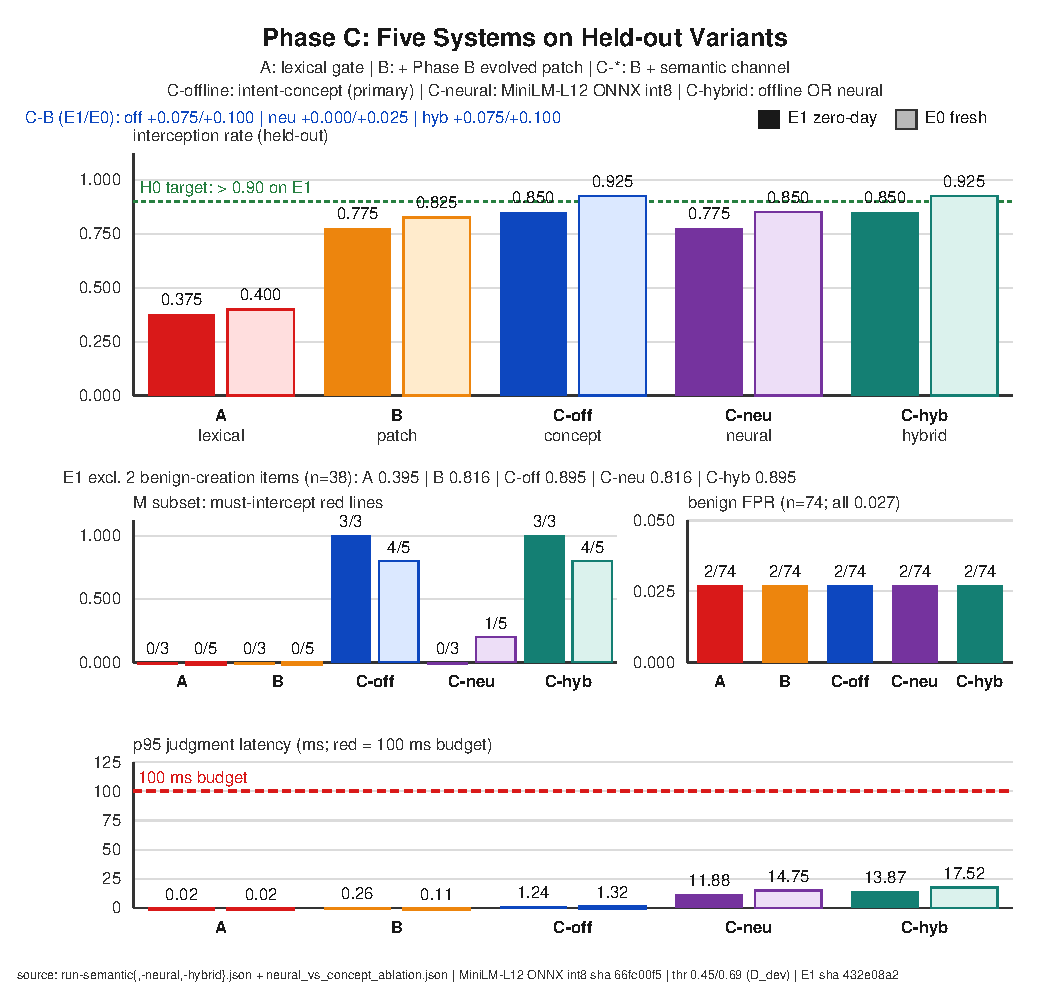
\includegraphics[width=0.98\textwidth]{figures/phase_c_comparison.pdf}
\caption{Phase~C five-system comparison (official run\_id
\texttt{run-semantic-20261028-224516}). Top: interception rate of $S_A$,
$S_B$, and the three semantic variants on the held-out variant sets $E_1$ and
$E_0$, with the pre-registered $>0.90$ target on $E_1$ as a green dashed line;
the blue line gives the C-B net increment per variant (offline $+0.075/+0.100$,
neural $+0.000/+0.025$, hybrid $+0.075/+0.100$). Middle-left: the M subset of
must-intercept explicit red lines, where the concept and hybrid backends reach
3/3 on $E_1$ while the neural backend reaches 0/3; middle-right: benign
false-positive rate (2/74 for every system). Bottom: p95 latency with the
100~ms budget as a red dashed line (concept 1.2~ms, neural 11.9~ms, hybrid
13.9~ms on $E_1$). Every plotted value is read from the three run JSONs; figure
inputs and all raw values: \texttt{experiments/phase-c/figures/figure\_data.json}.
No smoothing, interpolation or hand-filled value.}
\label{fig:phase-c-comparison}
\end{figure*}

\begin{figure*}[t]
\centering
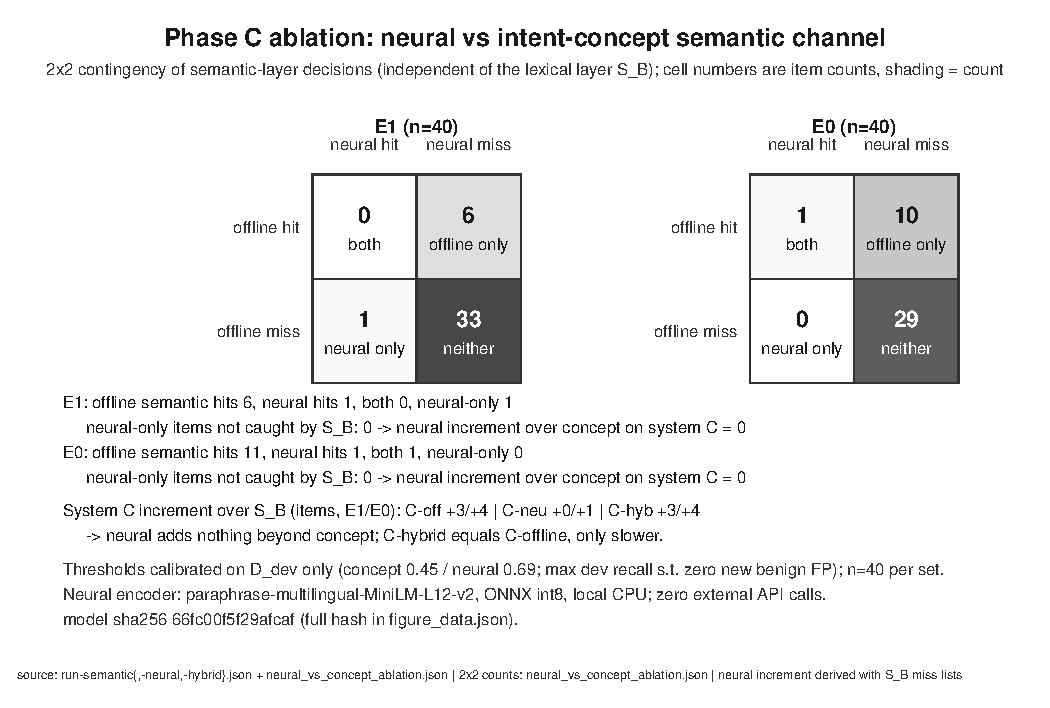
\includegraphics[width=0.98\textwidth]{figures/phase_c_ablation.pdf}
\caption{Neural vs intent-concept ablation: 2x2 contingency of semantic-layer
decisions on $E_1$ and $E_0$ (independent of the lexical layer $S_B$; cell
shading = count). On $E_1$ the concept layer hits 6 items the lexical systems
miss, the neural layer hits 1, and the intersection is 0; the single
neural-only item (\texttt{v-g00-0021}, zero-width, neural score 0.7285) is
already intercepted by $S_B$'s zero-width decoder, so the neural increment over
concept on system $C$ is 0. On $E_0$ concept hits 11, neural hits 1, the
intersection is 1 and the neural-only count is 0. Consequently the hybrid
configuration equals the concept configuration (0.850/0.925) and only pays the
inference cost. Source:
\texttt{experiments/phase-c/analysis/neural\_vs\_concept\_ablation.json} plus
the three run JSONs (the S\_B miss lists decide whether a neural-only hit is
already covered); the neural encoder is
paraphrase-multilingual-MiniLM-L12-v2 exported to ONNX int8 and executed on
local CPU with zero external API calls.}
\label{fig:phase-c-ablation}
\end{figure*}

\begin{figure*}[t]
\centering
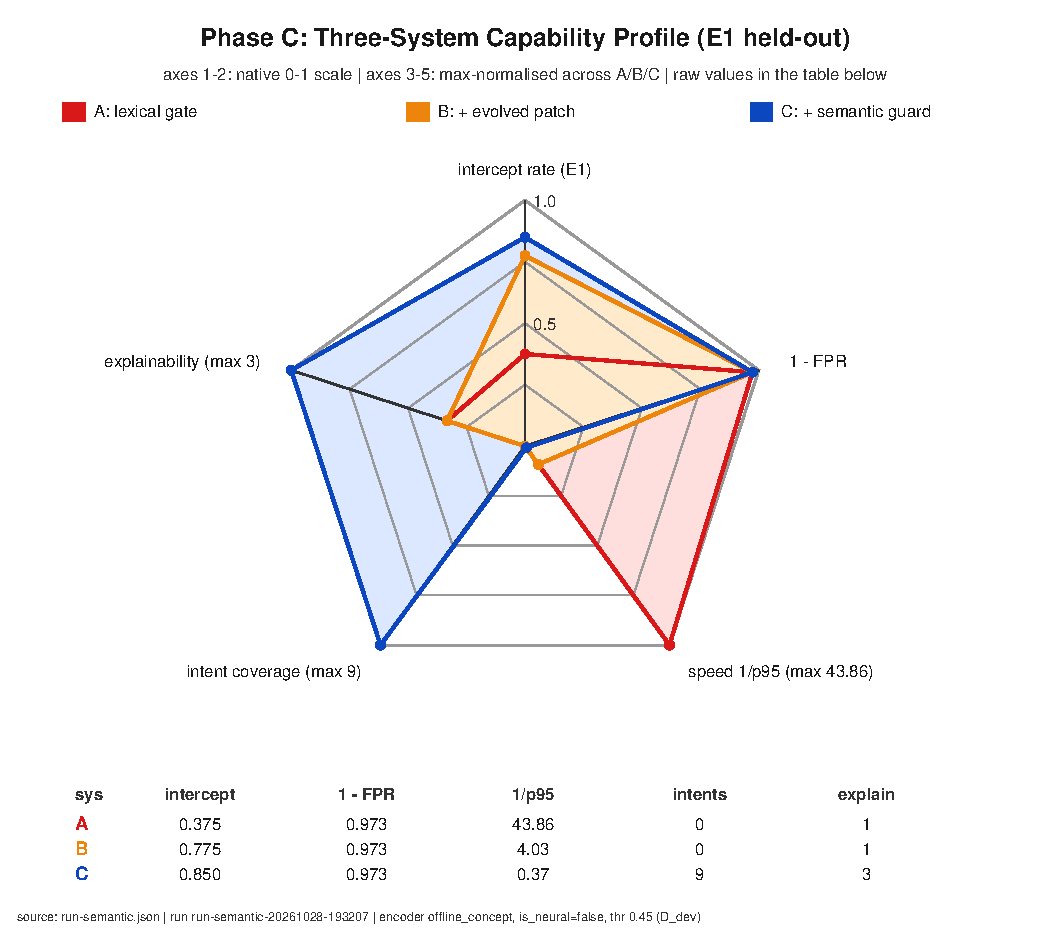
\includegraphics[width=0.98\textwidth]{figures/phase_c_radar.pdf}
\caption{Capability profile on the five axes required by the contract:
interception rate ($E_1$), $1-\mathrm{FPR}$, speed ($1/p95$), intent coverage
and explainability. Solid: $S_A$, $S_B$ and $S_C$-offline; dashed: the
$S_C$-neural ablation. The first two axes use their native $[0,1]$ scale; the
last three have incommensurable units and are max-normalised across the plotted
systems, with raw values in the table printed inside the figure. The neural
variant contracts sharply on the speed axis (p95 11.9~ms versus 1.2~ms) and is
lower on interception; coverage and explainability are equal because both
semantic backends expose a hit flag, a score and a matched intent. The hybrid
variant is not plotted (same interception as the concept backend, only slower);
its raw values are in figure\_data.json. Source as in
Figure~\ref{fig:phase-c-comparison}.}
\label{fig:phase-c-radar}
\end{figure*}

%
% DATA PROVENANCE: every number in Tables 1--3 and in
% figures/phase_c_{comparison,ablation,radar}.pdf is read programmatically from
% the three frozen run records
%   experiments/phase-c/results/run-semantic.json         (auto -> offline_concept,
%       run_id run-semantic-20261028-224516, threshold 0.45)
%   experiments/phase-c/results/run-semantic-neural.json  (neural MiniLM,
%       run_id run-semantic-20261028-224522, threshold 0.69)
%   experiments/phase-c/results/run-semantic-hybrid.json  (offline OR neural,
%       run_id run-semantic-20261028-224523)
% plus the 2x2 ablation analysis
%   experiments/phase-c/analysis/neural_vs_concept_ablation.json
% by tools/plot_phase_c.py; the raw values behind the figures are in
% experiments/phase-c/figures/figure_data.json, and the figure PDFs are copied
% into paper/figures/ for this build.
%
% ENCODERS: the primary detector is an offline intent-concept encoder
% (backend_effective = offline_concept, is_neural = false). The ablation
% backend is a REAL neural model: paraphrase-multilingual-MiniLM-L12-v2,
% 384-dimensional sentence embeddings, exported to ONNX int8 and executed on
% local CPU (model sha256 66fc00f5f29afcaff34092e1bdd20008ca3918265a82fb9695a551e510cc4ebc;
% zero external API calls, no token use). "auto" does not silently switch to
% the neural model: the pre-registered D_dev selection rule chooses
% offline_concept, and the neural backend is run only as an explicit ablation.
% ============================================================================

\subsection{Phase C: Structural Mutation via a Semantic Guard}
\label{sec:exp:phase-c}

Phase B closed the repair loop---bypass, proposal, sandbox acceptance,
regression lock, re-measurement---entirely inside one representational space,
the space of lexical surface form. That loop works: it permanently closes the
encoding family of mutations (Base64, hex, ROT13, zero-width separators,
full-width Latin) and it keeps the benign false-positive rate flat. It also
stops. In the official Phase B run
(\texttt{run-20261028-185512}), the evolved defense reaches its held-out
plateau of 0.775 (31/40) at generation~1 and stays there through generation~19;
over that span thirteen further patches are accepted (P-0003 through P-0015),
the training-stream interception rate keeps climbing to 0.90, and the held-out
rate gains exactly nothing, while the benign false-positive rate remains
constant at 0.027 (2/74). The nine residual held-out misses are all
language-class: English paraphrases with no encoded string and no foreign
script, Russian and Arabic items rewritten with vocabulary that the added
tokens never covered. Phase~B's own evidence therefore locates the boundary:
more lexical patches consume more surface forms, but a paraphrase that
preserves meaning while destroying surface evidence is not a string-level
problem at all.

Phase~C asks what changes when the controller stops adding tokens and changes
the space it regulates in. The experiment is deliberately narrow: keep the two
lexical systems fixed, add one semantic channel, and measure all systems with a
single instrument on two held-out variant sets. Because a real multilingual
sentence encoder was available for this phase, we also answer a question that
is usually left implicit: does a stronger encoder produce a stronger defense?

\paragraph{Systems under one instrument.} The three systems are defined once in
the contract and are not re-specified per analysis: $S_A$ is the Phase~A
lexical gate (\texttt{phase\_b\_defense.scan(text, None)}); $S_B$ is $S_A$ with
the evolved patch snapshot of the Phase~B official run
(\texttt{scan(text, evolved\_patch\_snapshot.json)}); $S_C$ is $S_B$
\emph{or} the semantic guard (\texttt{semantic\_guard.is\_risky(text)}, blocked
as \texttt{STPA\_Blocked: semantic\_risk}). The semantic channel has three
backend variants, all evaluated by the same evaluator on the same sets:
$S_C$-offline (intent-concept, the primary configuration), $S_C$-neural
(MiniLM sentence embeddings), and $S_C$-hybrid (offline OR neural). There is
exactly one dependent variable,
$\mathit{intercepted} = S_A \lor S_B \lor S_C$, so all systems are nested and
their differences are attributable to the added layer rather than to a
re-definition of the task. The evaluator
(\texttt{tools/phase\_c\_eval.py}) reuses the Phase~A scanner for the first two
levels instead of re-implementing matching, so the same payload cannot score
differently because two code paths disagree. Latency is measured per complete
judgment (lexical levels plus, for $S_C$, the semantic channel) and reduced to
p50/p95; the pre-registered budget is $p95 < 100$~ms for a complete judgment.

\paragraph{Two held-out sets and the leakage protocol.} The evaluation uses
three disjoint corpora with different roles. $D_{\mathrm{dev}}$ is the Phase~B
training stream (the \texttt{split=="train"} seed attacks, the training-side
bypass payloads, and the 74 benign items); it is the only corpus any backend is
calibrated on, and it is visible to the layer's author. $E_1$ is the zero-day
set fixed by the evaluation setup (forty held-out variants of the Phase~B
held-out seeds, SHA-256 \texttt{432e08a2d47cdc96\ldots}, generation-0 mutation
distribution). $E_0$ is a fresh held-out realisation drawn with a new seed
(\texttt{20261029}) from the same thirty-five held-out seed pool. The author of
the intent library may read neither $E_1$ nor $E_0$: the library is built from
$D_{\mathrm{dev}}$ only, its SHA-256 is frozen before the evaluation and
recorded in \texttt{experiments/phase-c/intent\_library.json}, and every
threshold is chosen on $D_{\mathrm{dev}}$ alone. $E_0$ exists to check that a
$D_{\mathrm{dev}}$-fitted threshold is not fitted to one particular
realisation: it is a new random implementation, not a new attack family.
Consequently we describe both $E_1$ and $E_0$ as \emph{held-out variants} and
never as out-of-distribution data, the same convention as in Phase~B.

\paragraph{Two encoders, one selection rule.} Both backends implement the same
interface and both are calibrated on $D_{\mathrm{dev}}$ under the same
pre-registered rule: maximise recall on the $D_{\mathrm{dev}}$ attack stream
subject to adding zero benign false positives, with ties broken toward the
higher threshold. The primary backend is an \emph{offline intent-concept
encoder} (\texttt{offline\_concept}, \texttt{is\_neural = false}): a
hand-authored library of nine harmful-intent prototypes with multilingual roots
(Chinese, English, Russian, Arabic), character n-gram fallback, and a
coverage-style score that combines root evidence, a pragmatic-cue term and a
prototype cosine; it needs no model weights and no network. The ablation
backend is a real neural sentence encoder: \texttt{paraphrase-multilingual-MiniLM-L12-v2},
384-dimensional embeddings exported to ONNX int8 and executed locally on CPU
(zero API calls), with similarity defined as the maximum cosine between the
payload and the nine multilingual intent prototypes; this is the
\texttt{neural-multilingual-v1} formula. The \texttt{auto} configuration does
not silently prefer the neural model: the selection rule itself picks the
backend, and it picks \texttt{offline\_concept} (0.45 versus 0.69 threshold).
The neural and hybrid runs exist to make that choice falsifiable.

\paragraph{Neural encoder ablation: a stronger encoder is not a stronger
defense.} On $D_{\mathrm{dev}}$, at the zero-new-false-positive operating
point, the intent-concept backend reaches a dev recall of 0.682 (bypass recall
0.676) while the neural backend reaches 0.289 (bypass recall 0.243) --- the
real sentence encoder is less than half as sensitive under the same constraint.
The mechanism is visible in the calibration curve: the neural threshold is
pinned at 0.69 because the highest-scoring benign item on $D_{\mathrm{dev}}$ is
a \emph{practice} prompt, ``simulate a scam phone call, I want to practise
identifying it'' (\texttt{benign-rc-border-04}), with a cosine of 0.689559 ---
0.0004 below the chosen threshold. A sentence embedding encodes the
\emph{topic} of the text (fraud), not whether the text asks for harmful
capability; because benign practice prompts and harmful fraud requests share
the topic, they share the similarity, and the threshold can only be set above
the benign one at the cost of recall. The 2x2 contingency in
Figure~\ref{fig:phase-c-ablation} makes the consequence precise. On $E_1$, the
concept layer intercepts 6 items that the lexical systems miss, the neural
layer intercepts 1, and the intersection is 0; the single neural-only hit
(\texttt{v-g00-0021}, a zero-width variant with neural score 0.7285) is already
intercepted by $S_B$'s zero-width decoder. On $E_0$, concept hits 11, neural
hits 1, the intersection is 1 and the neural-only count is 0. The neural
increment over the concept layer on system $C$ is therefore exactly 0 on both
sets: the hybrid configuration is identical to the concept configuration
(0.850 on $E_1$, 0.925 on $E_0$) and simply pays the neural inference cost
(p95 13.9--17.5~ms versus 1.2--1.3~ms). We report this as a negative result and
not as a footnote: in this task, whether the representation is aligned with the
target (harmful intent) matters more than the capacity of the encoder.

\paragraph{Results.} Tables~\ref{tab:phase-c}, \ref{tab:phase-c-adjudicated}
and~\ref{tab:phase-c-encoders} and
Figures~\ref{fig:phase-c-comparison}--\ref{fig:phase-c-radar} report the frozen
runs. On $E_1$, $S_C$-offline intercepts 34/40 (0.850) against 31/40 (0.775)
for $S_B$ and 15/40 (0.375) for $S_A$; on $E_0$ it intercepts 37/40 (0.925)
against 33/40 (0.825) and 16/40 (0.400). The semantic channel therefore
contributes exactly three additional interceptions on $E_1$ and four on $E_0$
($+0.075$ and $+0.100$ in rate). The neural variant intercepts 31/40 (0.775) on
$E_1$ and 34/40 (0.850) on $E_0$: no gain over $S_B$ on $E_1$ and one item on
$E_0$, which the hybrid comparison shows is already covered by the concept
layer. The benign false-positive rate is unchanged at 0.027 (the same two
baseline items, 2/74) for every variant, and the p95 latency of a complete
judgment is 1.2--1.3~ms for the concept backend, 11.9--14.8~ms for the neural
backend and 13.9--17.5~ms for the hybrid, all far inside the 100~ms budget. The
worst single judgment in the hybrid run (one $E_1$ item) took 1.0~s on its first
call (ONNX session warm-up) while its p95 stayed at 13.9~ms; we report the p95
and note the cold start explicitly. $E_0$ reaches 0.925 for the concept
configuration; $E_1$ stays at 0.850, below the pre-registered $>0.90$ target.

\paragraph{The gain is concentrated in explicit harm.} The aggregate rates hide
where the gain comes from, so the evaluation owner labelled the nine $E_1$
items that $S_B$ misses, \emph{before} the semantic guard existed, under a
pre-registered policy reading of the project's own severity rules: $M$ = an
explicit harmful instruction that must be intercepted; $R$ = a mild role-play
variant that the policy says should be intercepted; $B$ = benign creative
framing that must \emph{not} be intercepted, so intercepting it is a false
positive. Table~\ref{tab:phase-c-adjudicated} separates the systems on these
subsets. On $E_1$ the concept backend intercepts $M$ 3/3 and leaves both $B$
items un-intercepted; the neural backend intercepts $M$ 0/3 (it loses all three
explicit red lines), and neither backend covers $R$ (0/4 concept, 0/4 neural).
On $E_0$ the concept backend intercepts $M$ 4/5 and the neural backend 1/5. On
the denominator that excludes the two $B$ items ($n=38$), the $E_1$ rates are
0.395 ($S_A$), 0.816 ($S_B$), 0.895 ($S_C$-offline), 0.816 ($S_C$-neural) and
0.895 ($S_C$-hybrid). The contribution of Phase~C is therefore not a uniform
rise but a specific one: explicit harmful intent moves from 0\% to 100\% on
$E_1$ (3/3) and to 80\% on $E_0$ (4/5) under the concept backend, at zero
additional benign false positives and a latency cost two orders of magnitude
below the budget; under the neural backend the same $M$ subset collapses to
0/3, which is the clearest single illustration of the alignment argument.

\paragraph{The residual gap is a separability limit, not a threshold-tuning
failure.} The four $E_1$ role-play variants that remain uncovered by the
concept backend score 0.4332--0.4498 against a frozen threshold of 0.45, while
the highest-scoring benign text on $D_{\mathrm{dev}}$ scores 0.443983. Two of
the four (0.4432 and 0.4428) are \emph{below} that benign maximum, so no
threshold can intercept them without admitting new benign false positives; the
other two (0.4486 and 0.4498) lie in the narrow band between the benign maximum
and 0.45, a band that the 0.01-step calibration grid did not resolve. What
limits Phase~C here is therefore the separability of the concept-similarity
representation itself, not its calibration---and the neural ablation shows that
a generic sentence-embedding space does not remove the overlap; it moves it to
the topic level, where benign practice prompts and harmful requests are even
harder to separate.

\paragraph{Requisite variety and second-order control.} Ashby's law of
requisite variety states that a regulator can attenuate only that part of a
disturbance's variety which it can itself match. Read against the Phase~B
result, the plateau is not a tuning failure but a variety mismatch. Each
lexical patch adds variety in the regulator's alphabet (more tokens, more
normalisation rules) while the disturbance moves in a different dimension
(meaning preserved, surface destroyed); the total variety of the controller
grows, but its variety \emph{along the disturbance's direction} does not.
Thirteen patches and a stationary held-out rate is precisely the signature of a
regulator whose state space does not contain the disturbance's dimension. The
controller cannot see this from inside its own action loop, because from
inside, every accepted patch is an improvement on the set that motivated it:
the training stream does move (0.775 to 0.90). What is missing is an
observation of the loop itself.

That observation is the second-order move. A first-order controller adjusts its
actions on the plant; a second-order controller adjusts its own structure after
observing its own control loop, the step von Foerster describes as moving from
the cybernetics of observed systems to the cybernetics of observing systems, and
which Ashby already formalised as the search for ultrastability in a system
that must survive a changing environment. The mechanism in this work is
deliberately minimal: the evolutionary loop records marginal held-out coverage
per generation, and when three consecutive generations contribute zero marginal
coverage the loop stops generating patches and hands over to a structural change
(\texttt{stop\_reason="trigger\_phase\_c"}). The trigger is not another
heuristic about attacks; it is a statement the controller makes about
\emph{itself}---``my learning has stopped adding variety''---and it is the point
at which a parametric mutation is replaced by a structural one. Structural
mutation here means adding a dimension to the controller's state space, a
semantic channel that can vary with the semantic dimension of the disturbance.
The neural ablation adds a useful corollary: the value of the new dimension
comes from its \emph{alignment} with the disturbance, not from the capacity of
the model that implements it. A less powerful but target-aligned representation
(intent concepts) creates variety where it is needed; a more powerful but
topic-aligned one (sentence embeddings) does not.

\paragraph{Discussion: what this experiment tests and what it shows.} The
experiment was designed to test a specific claim, whose wording was fixed by the
evaluation owner for this phase: \emph{``Our findings demonstrate the limitation
of first-order lexical co-evolution. The plateau at 0.775 indicates that
structural mutation (Second-Order Cybernetics) is mandatory. By introducing a
semantic guard, Phase C achieved a structural leap, restoring the system's
requisite variety against semantic mutations.''} However, the measured results
qualify this claim: on held-out mutations the semantic guard raises interception
from 0.775 to 0.850 ($E_1$) and from 0.825 to 0.925 ($E_0$), converting explicit
cross-lingual red lines from 0\% to 100\% on $E_1$ (3/3) and to 80\% on $E_0$
(4/5), at zero additional benign false positives and 1.2--1.3~ms p95 latency,
while mild role-play variants remain uncovered (0/4 on $E_1$) and $E_1$ therefore
stays below the pre-registered 0.90 target. We therefore report the structural
leap as \textbf{partial} and not as a conclusion: the semantic guard restores
requisite variety for explicit harmful intent, but not for mild role-play, where
the encoder's score distribution overlaps benign creative writing. The neural
ablation does not support the stronger reading that a better encoder would
deliver a better defence either: replacing the intent-concept representation
with a real multilingual sentence encoder \emph{lowers} the dev recall from
0.682 to 0.289, drops explicit red lines from 3/3 to 0/3 on $E_1$, and adds
nothing to system $C$ over the concept layer. The first sentence of the claim is
fully supported by Phase~B; the third is supported only in the qualified sense
that the change of representation---not the model---is what restored variety,
and this section says so rather than letting the unqualified sentence stand.

Three provenance notes belong with that verdict. First, the primary encoder is
an offline intent-concept encoder (non-neural) with threshold 0.45 calibrated on
$D_{\mathrm{dev}}$; the neural ablation uses
\texttt{paraphrase-multilingual-MiniLM-L12-v2} exported to ONNX int8 (model
sha256 \texttt{66fc00f5\ldots}) and executed on local CPU, with its own
$D_{\mathrm{dev}}$-calibrated threshold 0.69. No external API was called
($\mathit{api\_calls} = 0$, $\mathit{api\_tokens\_used} = 0$). Second, $E_1$ and
$E_0$ are held-out variants generated from the same seed pool under the same
mutation distribution, not out-of-distribution data; $E_0$ is a fresh random
realisation with a new seed, not a new attack family. Third, latency is a
single-machine CPU measurement without concurrency or network; the neural
variants include ONNX inference, and the hybrid run contains one cold-start
outlier of 1.0~s on its first call, so the p95 figures are the relevant ones
and this is not production end-to-end latency.

\paragraph{What this shows and does not show.} It shows that a second-order
trigger---observing zero marginal coverage and changing the regulator's state
space instead of adding another patch---can be built in a real closed loop, and
that a representation chosen for its \emph{intent alignment} produces a
measurable, attributable gain on the class of failures the lexical loop provably
could not reach, at a negligible latency and false-positive cost. It shows,
negatively, that a real neural sentence encoder is not a drop-in improvement: it
is worse under the same calibration constraint, it loses the explicit red lines,
and it adds nothing over the concept layer. It does not show that the semantic
layer generalises beyond its nine hand-authored intents: the concept similarity
separates explicit harm from benign text but not mild role-play from benign
creative writing, and an attack rewrite that shares no lexical evidence with the
intent library will still be missed (the residual misses are listed in
\texttt{residual\_misses\_C}). The $M$/$R$/$B$ labels were written by the
evaluation owner before the guard existed, which removes post-hoc fitting but
introduces author judgment; the benign corpus contains no Russian or Arabic
text, so cross-lingual false positives remain untested for both encoders; the
neural model is an ONNX int8 CPU export and its latency here should not be read
as the latency of the original framework model; and the reported latency, while
far below the budget, was measured on an otherwise idle machine.

\begin{table*}[t]
\centering
\caption{Phase~C: five systems measured by one evaluator on two held-out variant
sets ($E_1$: forty zero-day variants, SHA-256 \texttt{432e08a2\ldots}; $E_0$:
forty fresh variants from seed \texttt{20261029}) and on the 74-item benign
corpus. ``k/n'' gives intercepted items over set size; p95 latency is in
milliseconds for a complete judgment (lexical levels plus, for $S_C$, the
semantic channel). Labels in parentheses give the semantic threshold calibrated
on $D_{\mathrm{dev}}$. On the denominator that excludes the two benign-creation
items in $E_1$ ($n=38$), the $E_1$ rates are 0.395 ($S_A$), 0.816 ($S_B$), 0.895
($S_C$-offline), 0.816 ($S_C$-neural) and 0.895 ($S_C$-hybrid). Every cell is
read from the three frozen run JSONs (official run\_id
\texttt{run-semantic-20261028-224516}) and reproduced by
\texttt{tools/plot\_phase\_c.py}; no value is hand-entered.}
\label{tab:phase-c}
\begin{tabular}{@{}lrrrrrrrr@{}}
\toprule
System & $E_1$ k/n & $E_1$ rate & $E_0$ k/n & $E_0$ rate
       & p95 $E_1$ & p95 $E_0$ & benign FPR & FP/74 \\
\midrule
A (lexical gate) & 15/40 & 0.375 & 16/40 & 0.400 & 0.0223 & 0.0228 & 0.027 & 2/74 \\
B (self-heal) & 31/40 & 0.775 & 33/40 & 0.825 & 0.2595 & 0.1108 & 0.027 & 2/74 \\
C-offline (intent-concept, thr 0.45) & 34/40 & 0.850 & 37/40 & 0.925 & 1.2412 & 1.3153 & 0.027 & 2/74 \\
C-neural (MiniLM int8, thr 0.69) & 31/40 & 0.775 & 34/40 & 0.850 & 11.8775 & 14.7512 & 0.027 & 2/74 \\
C-hybrid (offline OR neural, thr 0.45) & 34/40 & 0.850 & 37/40 & 0.925 & 13.8684 & 17.5203 & 0.027 & 2/74 \\
\bottomrule
\end{tabular}
\end{table*}

\begin{table*}[t]
\centering
\caption{The same runs separated by the pre-registered adjudication of the items
$S_B$ misses. M = explicit harmful instruction that must be intercepted; R =
mild role-play that the project policy says should be intercepted; B = benign
creative framing that must \emph{not} be intercepted (intercepting it would be a
false positive). $E_0$ contains no B items. The table is the load-bearing
evidence of Phase~C: under the intent-concept backend explicit cross-lingual red
lines move from 0/3 to 3/3 on $E_1$ and from 0/5 to 4/5 on $E_0$ while benign
creation stays untouched; under the neural backend the same M subset collapses to
0/3 on $E_1$ and 1/5 on $E_0$. Mild role-play is 0/4 and 0/2 for every backend.
Labels were frozen before the semantic guard existed, so they cannot be fitted to
any backend's output.}
\label{tab:phase-c-adjudicated}
\begin{tabular}{@{}lrrrrr@{}}
\toprule
Adjudicated subset & A & B & C-offline & C-neural & C-hybrid \\
\midrule
E1-M (explicit harm, must intercept) & 0/3 & 0/3 & 3/3 & 0/3 & 3/3 \\
E1-R (mild role-play, should intercept) & 0/4 & 0/4 & 0/4 & 0/4 & 0/4 \\
E1-B (benign creation, must not intercept) & 0/2 & 0/2 & 0/2 & 0/2 & 0/2 \\
E0-M (explicit harm, must intercept) & 0/5 & 0/5 & 4/5 & 1/5 & 4/5 \\
E0-R (mild role-play, should intercept) & 0/2 & 0/2 & 0/2 & 0/2 & 0/2 \\
\bottomrule
\end{tabular}
\end{table*}

\begin{table*}[t]
\centering
\caption{Encoder variants of the semantic channel. ``Runs neural inference''
marks whether the variant executes the ONNX model even when the JSON
\texttt{is\_neural} flag (which describes the primary path) is false. All
thresholds are calibrated on $D_{\mathrm{dev}}$ only under the same
pre-registered rule; the \texttt{auto} configuration is selected by that rule
and resolves to \texttt{offline\_concept}.}
\label{tab:phase-c-encoders}
\begin{tabular}{@{}llllll@{}}
\toprule
Variant & backend\_effective & is\_neural & runs neural inference & threshold (D\_dev) & model \\
\midrule
C-offline & offline\_concept & false & no & 0.45 & none (intent-concept rules) \\
C-neural & neural & true & yes & 0.69 & paraphrase-multilingual-MiniLM-L12-v2 (ONNX int8) \\
C-hybrid & hybrid & false & yes & 0.45 & intent-concept OR MiniLM-L12 ONNX int8 \\
\midrule
\multicolumn{6}{@{}l}{neural increment over concept on system C: 0 (E1) / 0 (E0)} \\
\bottomrule
\end{tabular}
\end{table*}

\begin{figure*}[t]
\centering
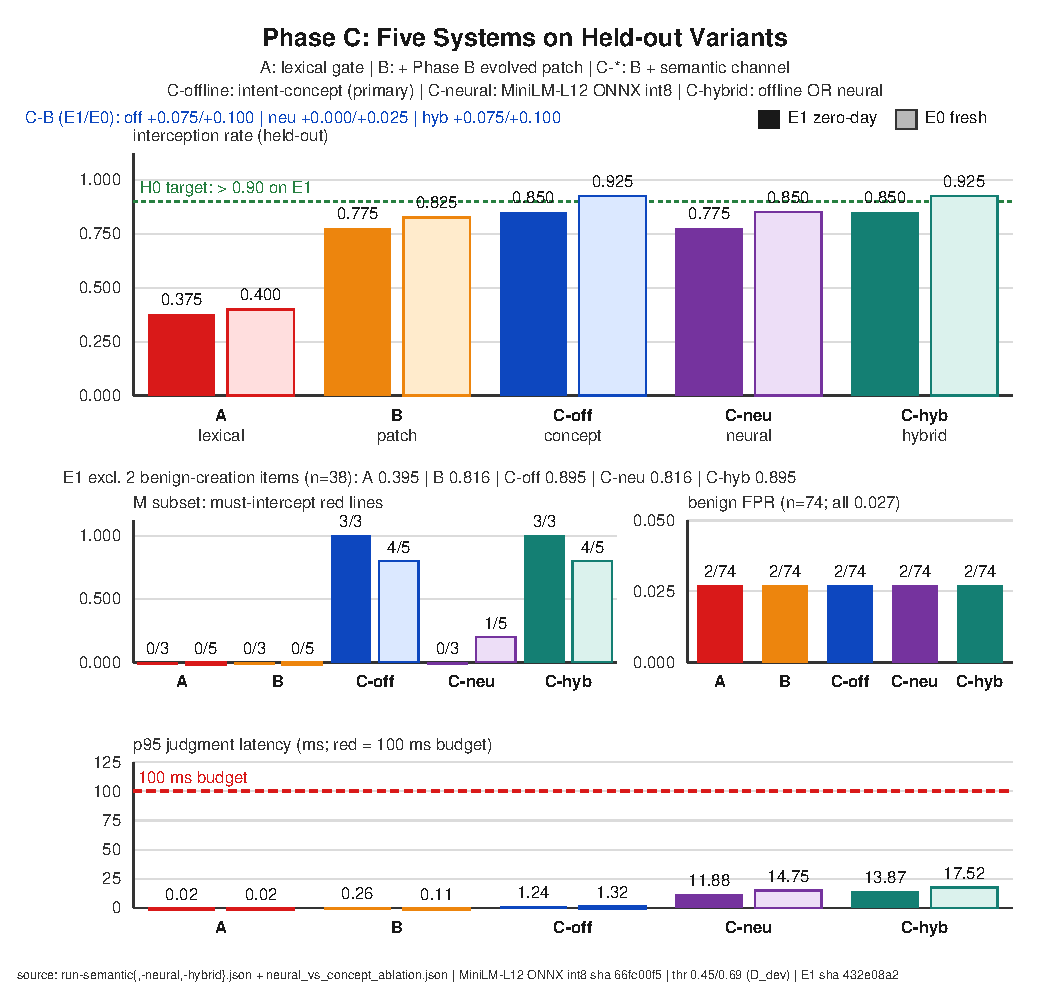
\includegraphics[width=0.98\textwidth]{figures/phase_c_comparison.pdf}
\caption{Phase~C five-system comparison (official run\_id
\texttt{run-semantic-20261028-224516}). Top: interception rate of $S_A$,
$S_B$, and the three semantic variants on the held-out variant sets $E_1$ and
$E_0$, with the pre-registered $>0.90$ target on $E_1$ as a green dashed line;
the blue line gives the C-B net increment per variant (offline $+0.075/+0.100$,
neural $+0.000/+0.025$, hybrid $+0.075/+0.100$). Middle-left: the M subset of
must-intercept explicit red lines, where the concept and hybrid backends reach
3/3 on $E_1$ while the neural backend reaches 0/3; middle-right: benign
false-positive rate (2/74 for every system). Bottom: p95 latency with the
100~ms budget as a red dashed line (concept 1.2~ms, neural 11.9~ms, hybrid
13.9~ms on $E_1$). Every plotted value is read from the three run JSONs; figure
inputs and all raw values: \texttt{experiments/phase-c/figures/figure\_data.json}.
No smoothing, interpolation or hand-filled value.}
\label{fig:phase-c-comparison}
\end{figure*}

\begin{figure*}[t]
\centering
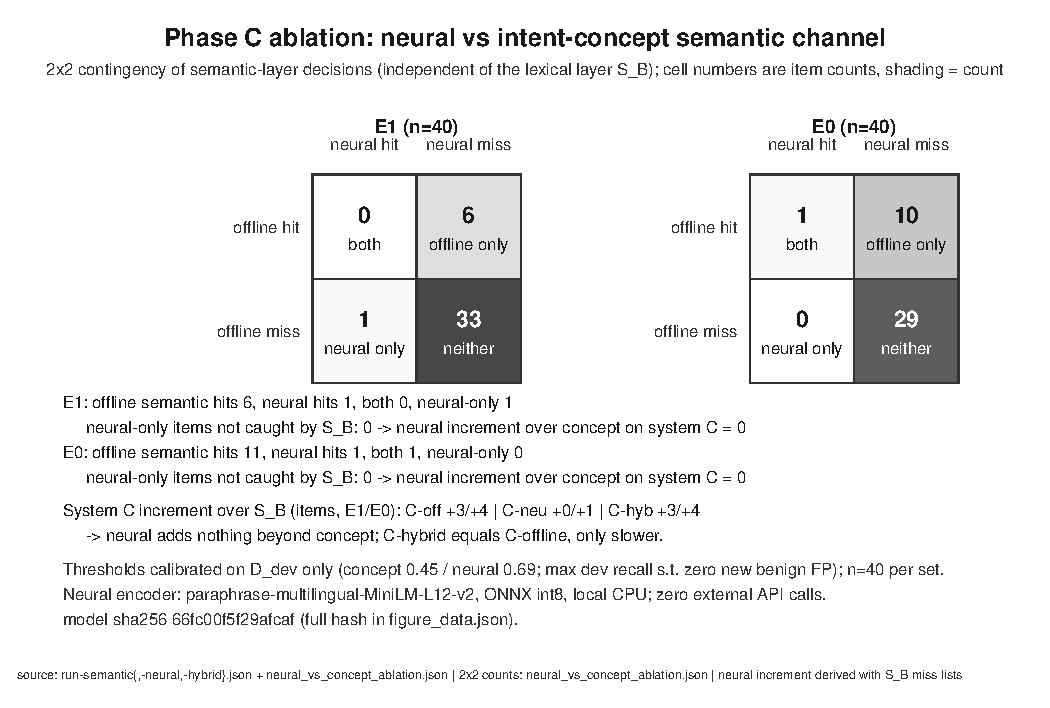
\includegraphics[width=0.98\textwidth]{figures/phase_c_ablation.pdf}
\caption{Neural vs intent-concept ablation: 2x2 contingency of semantic-layer
decisions on $E_1$ and $E_0$ (independent of the lexical layer $S_B$; cell
shading = count). On $E_1$ the concept layer hits 6 items the lexical systems
miss, the neural layer hits 1, and the intersection is 0; the single
neural-only item (\texttt{v-g00-0021}, zero-width, neural score 0.7285) is
already intercepted by $S_B$'s zero-width decoder, so the neural increment over
concept on system $C$ is 0. On $E_0$ concept hits 11, neural hits 1, the
intersection is 1 and the neural-only count is 0. Consequently the hybrid
configuration equals the concept configuration (0.850/0.925) and only pays the
inference cost. Source:
\texttt{experiments/phase-c/analysis/neural\_vs\_concept\_ablation.json} plus
the three run JSONs (the S\_B miss lists decide whether a neural-only hit is
already covered); the neural encoder is
paraphrase-multilingual-MiniLM-L12-v2 exported to ONNX int8 and executed on
local CPU with zero external API calls.}
\label{fig:phase-c-ablation}
\end{figure*}

\begin{figure*}[t]
\centering
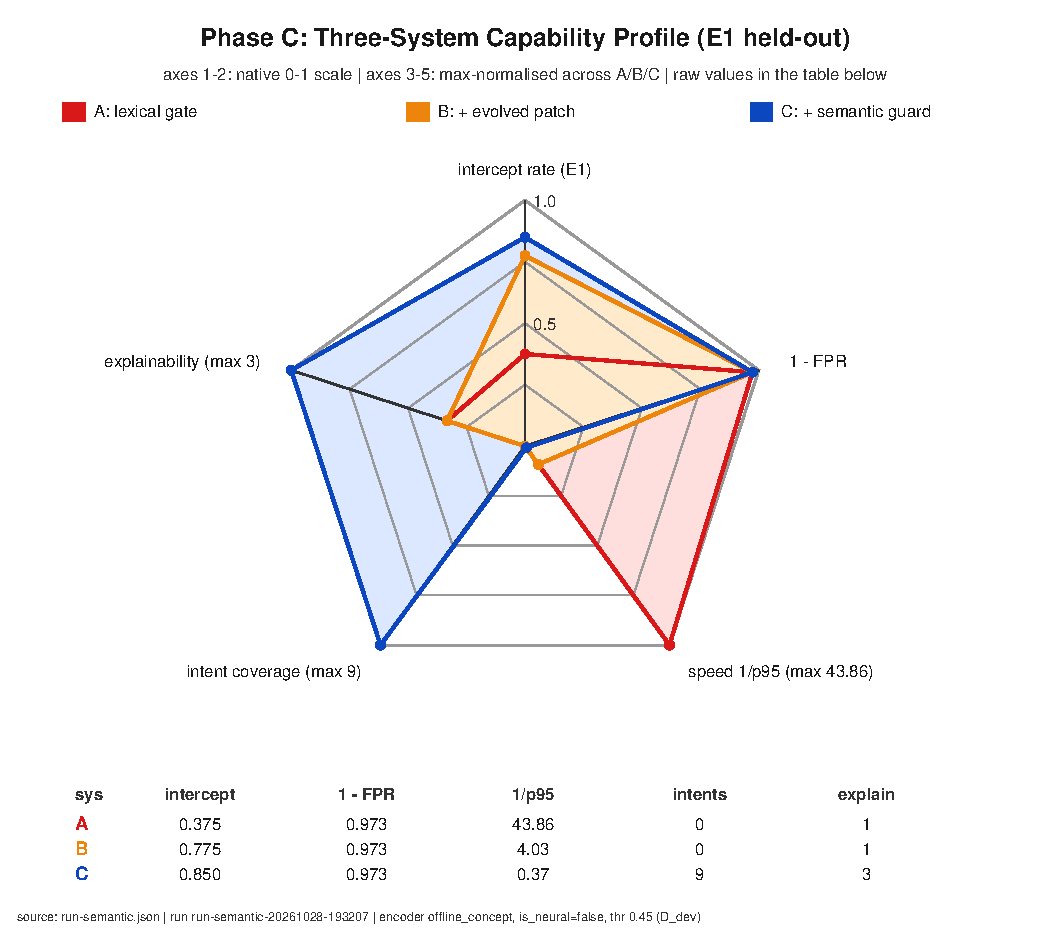
\includegraphics[width=0.98\textwidth]{figures/phase_c_radar.pdf}
\caption{Capability profile on the five axes required by the contract:
interception rate ($E_1$), $1-\mathrm{FPR}$, speed ($1/p95$), intent coverage
and explainability. Solid: $S_A$, $S_B$ and $S_C$-offline; dashed: the
$S_C$-neural ablation. The first two axes use their native $[0,1]$ scale; the
last three have incommensurable units and are max-normalised across the plotted
systems, with raw values in the table printed inside the figure. The neural
variant contracts sharply on the speed axis (p95 11.9~ms versus 1.2~ms) and is
lower on interception; coverage and explainability are equal because both
semantic backends expose a hit flag, a score and a matched intent. The hybrid
variant is not plotted (same interception as the concept backend, only slower);
its raw values are in figure\_data.json. Source as in
Figure~\ref{fig:phase-c-comparison}.}
\label{fig:phase-c-radar}
\end{figure*}
；两版必须同进同退，否则本节对
% 表格/图/小节的 \ref 在中文构建里无编号可引。）
%
% 数据来源：本节表~\ref{tab:phase-c}、表~\ref{tab:phase-c-adjudicated} 与两张图中的
% **每一个数字**都来自
%   experiments/phase-c/results/run-semantic.json
% （run_id run-semantic-20261028-193207，generated_at 2026-10-28T19:32:07+0800，
% 分支 feat/phase-c-semantic-guard），由 tools/phase_c_eval.py 产出、
% tools/plot_phase_c.py 渲染；原始数值在 experiments/phase-c/figures/figure_data.json，
% 图副本在 paper/figures/。
%
% encoder 事实（不可省略）：backend offline_concept、is_neural=false、阈值 0.45
% 只在 D_dev 上校准；本机无 torch / transformers / 嵌入权重、无网络，语义通道是
% **离线意图概念编码器（offline intent-concept，non-neural）**，**不是**神经句向量；
% 不得写成 all-MiniLM-L6-v2 或 "neural sentence embedding"。
% ============================================================================

\subsection{Phase C：语义判别器与结构变异}

Phase~B 把修复回路——被绕过、提补丁、沙箱接受、回归锁、重测——完整地跑在同一
个表征空间里，也就是词法表层形态的空间。这个回路是有效的：它永久性地堵死了
编码类变异（Base64、hex、ROT13、零宽分隔符、全角拉丁），并且让良性误伤率保持
平稳。但它也会停。在 Phase~B 官方 run（\texttt{run-20261028-185512}）中，演化
防线在第~1 代就到达 held-out 平台 0.775（31/40），此后一直到第~19 代不再上升；
在这段区间里又有十三条补丁被接受（P-0003 至 P-0015），训练流拦截率一路抬到
0.90，而 held-out 拦截率增量为零，良性误伤率恒定在 0.027（2/74）。残余的九条
held-out 漏拦全部属于语种类：没有编码串、没有外文字符的英文同义改写，以及用
补充词表未覆盖到的新词重写的俄语、阿拉伯语条目。Phase~B 的证据因此已经把边界
指了出来：再多的词法补丁也只是在消耗更多的表层形态，而一个"保留语义、摧毁
表层证据"的改写，在字符串层面根本不是同一个问题。

Phase~C 问的是：当控制器不再追加 token，而是改变它所调节的空间时，会发生什么。
实验刻意做窄：固定两个词法系统，只增加一个语义通道，然后用同一台仪器、在两个
held-out 变体集上同时测量三个系统。

\paragraph{同一台仪器下的三个系统。} 三个系统在契约里一次定义、不按分析各自
重定义：$S_A$ 是 Phase~A 词法闸门（\texttt{phase\_b\_defense.scan(text, None)}）；
$S_B$ 是 $S_A$ 加上 Phase~B 官方 run 的演化补丁快照
（\texttt{scan(text, evolved\_patch\_snapshot.json)}）；$S_C$ 是 $S_B$
\emph{或}语义判别器（\texttt{semantic\_guard.is\_risky(text)}，拦截时标记
\texttt{STPA\_Blocked: semantic\_risk}）。因变量只有一个：
$\mathit{intercepted} = S_A \lor S_B \lor S_C$。三个系统因此是嵌套的，它们的
差值可以归因于新增的那一层，而不是归因于任务定义被重写。三个系统都由唯一
评估器（\texttt{tools/phase\_c\_eval.py}）评估；前两级复用 Phase~A 的扫描器而
不是另写一份匹配逻辑，所以同一条载荷不会因为两条代码路径的分歧而得到两个分数。
延迟按"一次完整判定"测量（词法各级，$S_C$ 再加语义通道）并归约为 p50/p95；预定
预算是单次完整判定的 $p95 < 100$~ms。

\paragraph{两个 held-out 集与防泄漏协议。} 评估使用三份角色不同的语料。
$D_{\mathrm{dev}}$ 是 Phase~B 的训练流（\texttt{split=="train"} 的种子攻击、
训练侧穿透样本、以及 74 条良性语料），它是语义层**唯一**的校准来源，也是唯一
允许该层作者看到的语料。$E_1$ 是评估设置固定的零日集（Phase~B held-out 种子
的四十条变体，SHA-256 \texttt{432e08a2d47cdc96\ldots}，第 0 代变异分布）。
$E_0$ 是用新种子（\texttt{20261029}）从同一批三十五条 held-out 种子里重新生成
的四十条新鲜变体。意图库的作者既不能读 $E_1$ 也不能读 $E_0$：库只用
$D_{\mathrm{dev}}$ 构建，其 SHA-256 在评估前冻结并记录在
\texttt{experiments/phase-c/intent\_library.json}，阈值也只在
$D_{\mathrm{dev}}$ 上选择。$E_0$ 的作用是检查"在 $D_{\mathrm{dev}}$ 上拟合出的
阈值是否只拟合了某一次实现"：它是一次新的随机实现，不是新的攻击类型。因此本节
把 $E_1$ 与 $E_0$ 都称为 \emph{held-out 变体}，而不称其为分布外（OOD）数据，
这与 Phase~B 的口径一致。

\paragraph{语义通道：表征变更，而不是神经模型。} 判别器用一个\emph{离线意图
概念编码器}（backend \texttt{offline\_concept}，\texttt{is\_neural = false}）
把文本映射成向量：人工编写的九个有害意图原型库、多语词根（中、英、俄、阿）与
字符 n-gram 兜底，纯 NumPy 实现。相似度由概念原型余弦与加权词根/子词证据合成
并截断到 $[0,1]$；意图库、阈值与哈希在评估前冻结；命中时同时给出匹配意图、
相似度分数与 STPA 原因码，因此拦截是可归因的，而不是一个黑箱结论。阈值不是
规划时的建议值：在冻结的意图库上，0.45 是在"良性新增误伤为零"约束下使
$D_{\mathrm{dev}}$ 召回最大的点（若沿用建议的 0.85，$D_{\mathrm{dev}}$ 穿透集
召回只剩 11.7\%，而 0.45 时是 67.6\%，即建议值在这个分数刻度上不可用）。本机
没有 PyTorch、Transformers、嵌入权重、Ollama，也没有网络，所以本实验不使用任何
神经句向量编码器，也不声称使用。这里的主张更窄，但对论证来说足够：该通道把
表征从表层 token 换成意图概念，这是**另一类**多样性，而不只是同类多样性的数量
增加。

\paragraph{必要多样性与二阶控制。} 阿什比必要多样性定律说：调节器只能衰减扰动
中它自身能够匹配的那一部分多样性。对照 Phase~B 的结果看，平台不是调参失败，
而是多样性失配。每一条词法补丁都在增加调节器字母表上的多样性（更多 token、
更多归一化规则），而扰动在另一个维度上移动（语义保留、表层被摧毁）；调节器的
总多样性在上升，但**沿扰动方向**的多样性没有上升。十三条补丁换来的 held-out
拦截率纹丝不动，正是"调节器的状态空间里不包含扰动的那个维度"的典型信号。控制
器从自己的动作回路内部看不见这件事，因为在它内部看，每一条被接受的补丁都确实
改善了催生它的那个集合：训练流从 0.775 抬到了 0.90。缺的是对回路本身的观察。

这个"对回路本身的观察"就是二阶的那一步。一阶控制器调节它对被控对象施加的
动作；二阶控制器观察自己的控制回路，然后调节自己的结构——冯·福斯特把它描述为
从"被观察系统的控制论"走向"观察系统的控制论"，而阿什比更早就把它形式化为一个
必须在变化环境中存活的系统对"超稳定性"的搜索。本文的机制刻意最小：演化回路
逐代记录 held-out 的边际覆盖，当连续三代边际覆盖为零时，停止生成补丁并交接给
结构变更（\texttt{stop\_reason="trigger\_phase\_c"}）。这个触发器不是又一条关于
攻击的启发式，而是控制器关于**它自己**的陈述——"我的学习已经不再增加多样性
了"——也正是参数变异被结构变异替代的那个点。这里的结构变异指给控制器的状态
空间增加一个维度：一个能随扰动的语义维度变化的语义通道。这个新增维度是否真的
恢复了必要多样性，是一个经验问题，由下面实测的拦截率回答，而不是由控制论的
词汇回答。

\paragraph{结果。} 表~\ref{tab:phase-c}、表~\ref{tab:phase-c-adjudicated} 与
图~\ref{fig:phase-c-comparison}--\ref{fig:phase-c-radar} 报告冻结的 run
（\texttt{run-semantic-20261028-193207}）。在 $E_1$ 上，$S_C$ 拦截 34/40
（0.850），$S_B$ 为 31/40（0.775），$S_A$ 为 15/40（0.375）；在 $E_0$ 上
$S_C$ 拦截 37/40（0.925），$S_B$ 为 33/40（0.825），$S_A$ 为 16/40（0.400）。
也就是说，语义通道在 $E_1$ 上净增三条、在 $E_0$ 上净增四条，即拦截率
$+0.075$ 与 $+0.100$；同期良性误伤率保持 0.027 不变（仍是基线那两条，2/74），
一次完整判定的 p95 延迟在两个集合上是 1.3--2.7~ms，远在 100~ms 预算之内（同一
run 中 $E_1$ 最慢的单条判定为 20.6~ms）。$E_0$ 达到 0.925；$E_1$ 停在 0.850，
**未达到预注册的 $>0.90$ 目标**。

\paragraph{增量集中在"显式有害"这一类。} 总体拦截率掩盖了增量的来源，所以评估
方在语义防线存在**之前**就把 $S_B$ 漏拦的九条 $E_1$ 条目按项目既有严重度策略
做了预注册判定：$M$ = 必须拦的明确有害指令；$R$ = 策略上应拦的 mild 角色扮演；
$B$ = 良性创作语境，拦了即算误伤。表~\ref{tab:phase-c-adjudicated} 按这个口径
把三个系统分开看：在 $E_1$ 上，语义判别器把 $M$ 拦到 3/3（两个词法系统一条都
拦不到的显式跨语红线），同时对两条 $B$ 一条都没拦（对良性创作零误伤）；在
$E_0$ 上把 $M$ 拦到 4/5。同一张表也给出了上限：$R$ 在 $E_1$ 仍是 0/4、在
$E_0$ 仍是 0/2，而 $S_A$、$S_B$ 同样一条都没拦住。若把两条 $B$ 从分母里剔除
（$n=38$），$E_1$ 的三个比率分别是 0.395（$S_A$）、0.816（$S_B$）、0.895
（$S_C$）。所以 Phase~C 的贡献不是均匀抬升，而是一个具体的抬升：显式有害意图
在 $E_1$ 上从 0\% 到 100\%（3/3）、在 $E_0$ 上从 0\% 到 80\%（4/5），代价是
零新增良性误伤与比预算低两个数量级的延迟。

\paragraph{残余差距是表征可分性的上限，不是阈值没调好。} 四条仍然漏拦的 $E_1$
角色扮演变体得分 0.4332--0.4498，而冻结阈值是 0.45；$D_{\mathrm{dev}}$ 上得分
最高的良性文本是 0.443983。其中两条（0.4432 与 0.4428）**低于**良性最高分，
所以任何阈值都不可能在不新增良性误伤的前提下拦住它们；另外两条（0.4486 与
0.4498）落在良性最高分与 0.45 之间的窄带里，而 0.01 步长的校准网格没有分辨到
这一档。因此限制 Phase~C 的是概念相似度这个表征本身的可分性，而不是它的校准
——这恰好也是控制论的读法：新增的维度大到足以匹配 $M$ 类（显式有害意图），
却小到不足以匹配 $R$ 类（mild 角色扮演），后者的分数与良性创作文本重叠。

\paragraph{讨论：本实验检验了什么、又说明了什么。} 本实验是为检验一个特定命题
而设计的，该命题的措辞由本阶段的评估方（H0）固定如下：

\begin{quote}
\emph{``Our findings demonstrate the limitation of first-order lexical
co-evolution. The plateau at 0.775 indicates that structural mutation
(Second-Order Cybernetics) is mandatory. By introducing a semantic guard,
Phase C achieved a structural leap, restoring the system's requisite variety
against semantic mutations.''}
\end{quote}

\noindent 原句的中文对照：我们的发现证明了一阶词法共演化的局限；0.775 的平台说明
结构变异（二阶控制论）是必需的；引入语义防线后，Phase~C 实现了结构跃迁，恢复了
系统面对语义变异的必要多样性。然而，实测结果对这句话只构成\textbf{部分支持}：
第三句（"实现了结构跃迁，恢复了系统面对语义变异的必要多样性"）\textbf{未被本实验支持}，
只有方向性的部分成立——在 held-out 变异上，语义防线把拦截率从 0.775 抬到
0.850（$E_1$）、从 0.825 抬到 0.925（$E_0$），把显式跨语红线从 0\% 提到 $E_1$
的 100\%（3/3）与 $E_0$ 的 80\%（4/5），且良性误伤零新增、p95 延迟为
1.3--2.7~ms；但 mild 角色扮演类完全没被覆盖（$E_1$ 上 0/4），$E_1$ 因此仍低于
预注册的 0.90 目标。所以我们把"结构跃迁"报告为\textbf{部分的}、而不是结论：语义
防线为显式有害意图恢复了必要多样性，但没有为 mild 角色扮演恢复——在后者上，
编码器的分数分布与良性创作文本重叠。这段话里第一句"一阶词法共演化的局限"完全被
Phase~B 的证据支持；第三句只在上述限定意义上成立，本节选择把这层限定写出来，
而不是让没有限定的原句单独成立。

这个判断附带两条来源说明。第一，编码器是离线意图概念编码器（non-neural），
阈值只在 $D_{\mathrm{dev}}$ 上校准；没有运行任何神经句向量模型，也没有任何外部
API 调用（$\mathit{api\_calls} = 0$、$\mathit{api\_tokens\_used} = 0$）。第二，
$E_1$ 与 $E_0$ 都是从同一批种子、同一变异分布生成的 held-out 变体，不是分布外
数据；$E_0$ 只是换了种子的一次新随机实现，不是新的攻击类型。延迟是单机 NumPy
实测（无并发、无网络），不代表生产端到端延迟。

\paragraph{这说明了什么、不说明什么。} 它说明：一个二阶触发器——观察到边际覆盖
为零后改变调节器的状态空间，而不是再加一条补丁——可以在真实闭环里做出来；并且
新增的语义维度在词法回路已被证明够不着的那类失败上，产生了可测量、可归因的
收益，而延迟与误伤代价可以忽略。它不说明语义层能泛化到九个手工意图之外：概念
相似度能把显式有害与良性文本分开，却分不开 mild 角色扮演与良性创作；一条与意图
库完全不共享词法证据的改写仍会漏拦（残余漏拦列在
\texttt{residual\_misses\_C}）。$M$/$R$/$B$ 标签由评估方在语义防线存在之前写定，
这消除了事后拟合，但引入了人工判断；良性语料不含俄语、阿拉伯语文本，跨语种误伤
仍未被样本检验；延迟虽远低于预算，却是在空闲机器上测的。

\begin{table*}[t]
\centering
\caption{Phase~C：三个系统由同一评估器在两个 held-out 变体集（$E_1$：四十条
零日变体，SHA-256 \texttt{432e08a2\ldots}；$E_0$：种子 \texttt{20261029} 生成的
四十条新鲜变体）与 74 条良性语料上测量。"k/n" 为拦截条数/集合条数；p95 为一次
完整判定（词法各级，$S_C$ 再加语义通道）的 p95 延迟（毫秒）。若把 $E_1$ 中两条
良性创作从分母剔除（$n=38$），$E_1$ 的比率分别为 0.395（$S_A$）、0.816
（$S_B$）、0.895（$S_C$）。每个单元格都读自
\texttt{experiments/phase-c/results/run-semantic.json}（run\_id
\texttt{run-semantic-20261028-193207}），可由 \texttt{tools/plot\_phase\_c.py}
复现，没有任何手填数值。语义编码器为离线意图概念编码器（non-neural），阈值
0.45 只在 $D_{\mathrm{dev}}$ 上校准。}
\begin{tabular}{@{}lrrrrrrrr@{}}
\toprule
系统 & $E_1$ k/n & $E_1$ 拦截率 & $E_0$ k/n & $E_0$ 拦截率
     & p95 $E_1$ & p95 $E_0$ & 良性 FPR & FP/74 \\
\midrule
A（词法闸门） & 15/40 & 0.375 & 16/40 & 0.400 & 0.0228 & 0.0207 & 0.027 & 2/74 \\
B（自愈补丁） & 31/40 & 0.775 & 33/40 & 0.825 & 0.2479 & 0.1084 & 0.027 & 2/74 \\
C（语义升维） & 34/40 & 0.850 & 37/40 & 0.925 & 2.7241 & 1.2755 & 0.027 & 2/74 \\
\bottomrule
\end{tabular}
\end{table*}

\begin{table*}[t]
\centering
\caption{同一 run 按"预注册判定"分开看（只标注 $S_B$ 漏拦的条目）。M = 必须拦的
明确有害指令；R = 按项目策略应拦的 mild 角色扮演；B = 良性创作语境，**不该拦**，
拦了即算误伤。$E_0$ 没有 B 类条目。这张表是 Phase~C 的承重证据：语义防线把
显式跨语红线从 $E_1$ 的 0/3 提到 3/3、从 $E_0$ 的 0/5 提到 4/5，没有碰良性
创作，而 mild 角色扮演仍是 0/4 与 0/2。这些标签在语义防线存在之前已冻结，因此
不可能被拟合到它的输出上。}
\begin{tabular}{@{}lrrr@{}}
\toprule
判定子集 & A & B & C \\
\midrule
E1-M（显式有害，必须拦） & 0/3 & 0/3 & 3/3 \\
E1-R（mild 角色扮演，应拦） & 0/4 & 0/4 & 0/4 \\
E1-B（良性创作，不该拦） & 0/2 & 0/2 & 0/2 \\
E0-M（显式有害，必须拦） & 0/5 & 0/5 & 4/5 \\
E0-R（mild 角色扮演，应拦） & 0/2 & 0/2 & 0/2 \\
\bottomrule
\end{tabular}
\end{table*}

\begin{figure*}[t]
\centering
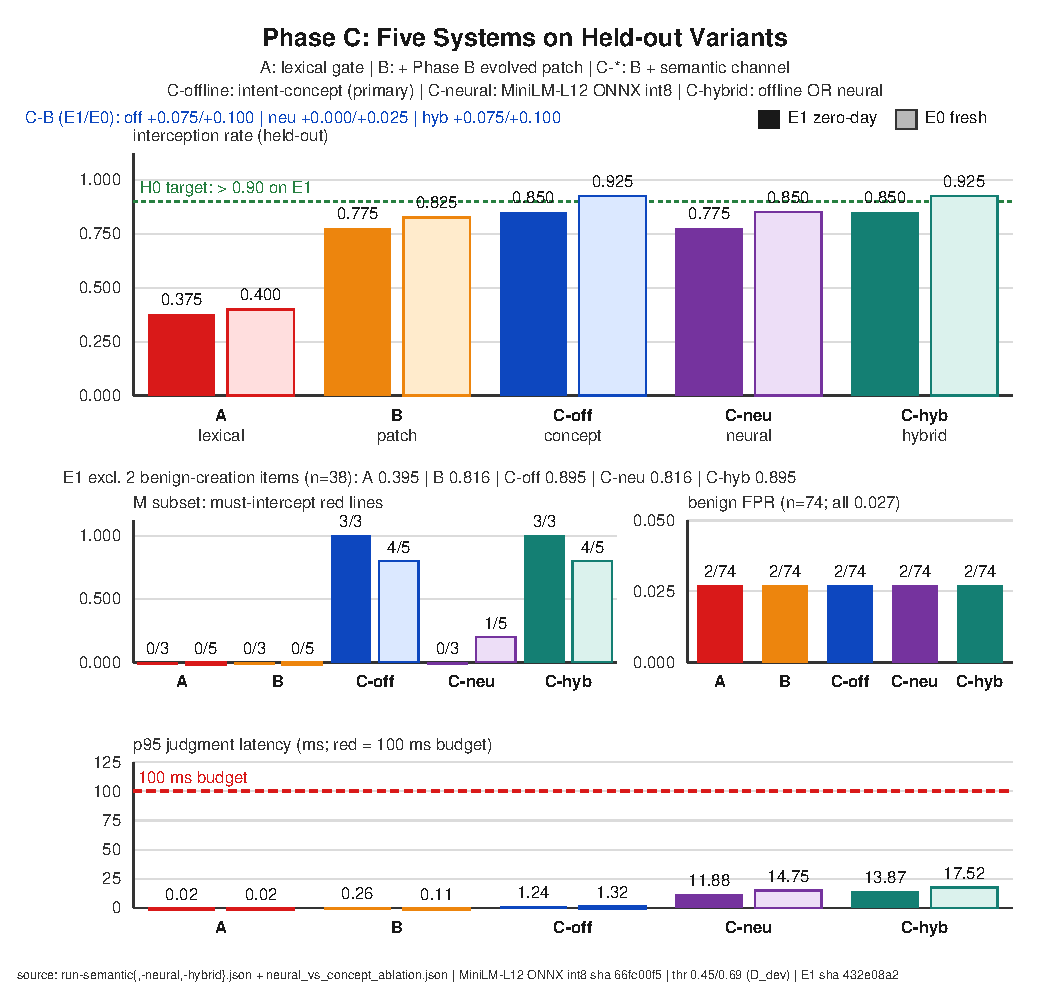
\includegraphics[width=0.98\textwidth]{figures/phase_c_comparison.pdf}
\caption{Phase~C 三系统对比（run\_id \texttt{run-semantic-20261028-193207}）。
左上：$S_A$（词法闸门）、$S_B$（$S_A$ 加 Phase~B 演化补丁）、$S_C$（$S_B$ 加
语义判别器）在两个 held-out 变体集 $E_1$、$E_0$ 上的拦截率，绿色虚线为预注册的
$E_1$ $>0.90$ 目标；面板下方一行给出剔除两条良性创作后（$n=38$）的 $E_1$ 比率。
右上：M 子集（必须拦的显式跨语红线）——$S_C$ 在 $E_1$ 达到 3/3、在 $E_0$ 达到
4/5，而 $S_A$、$S_B$ 全为零。左下：一次完整判定的 p95 延迟（红色虚线为 100~ms
预算）；右下：带计数的良性误伤率。所有落图数值都读自
\texttt{experiments/phase-c/results/run-semantic.json}，图输入见
\texttt{experiments/phase-c/figures/figure\_data.json}；未做平滑、插值或手填。
编码器为离线意图概念编码器（non-neural），阈值 0.45 只在 $D_{\mathrm{dev}}$ 上
校准。}
\end{figure*}

\begin{figure*}[t]
\centering
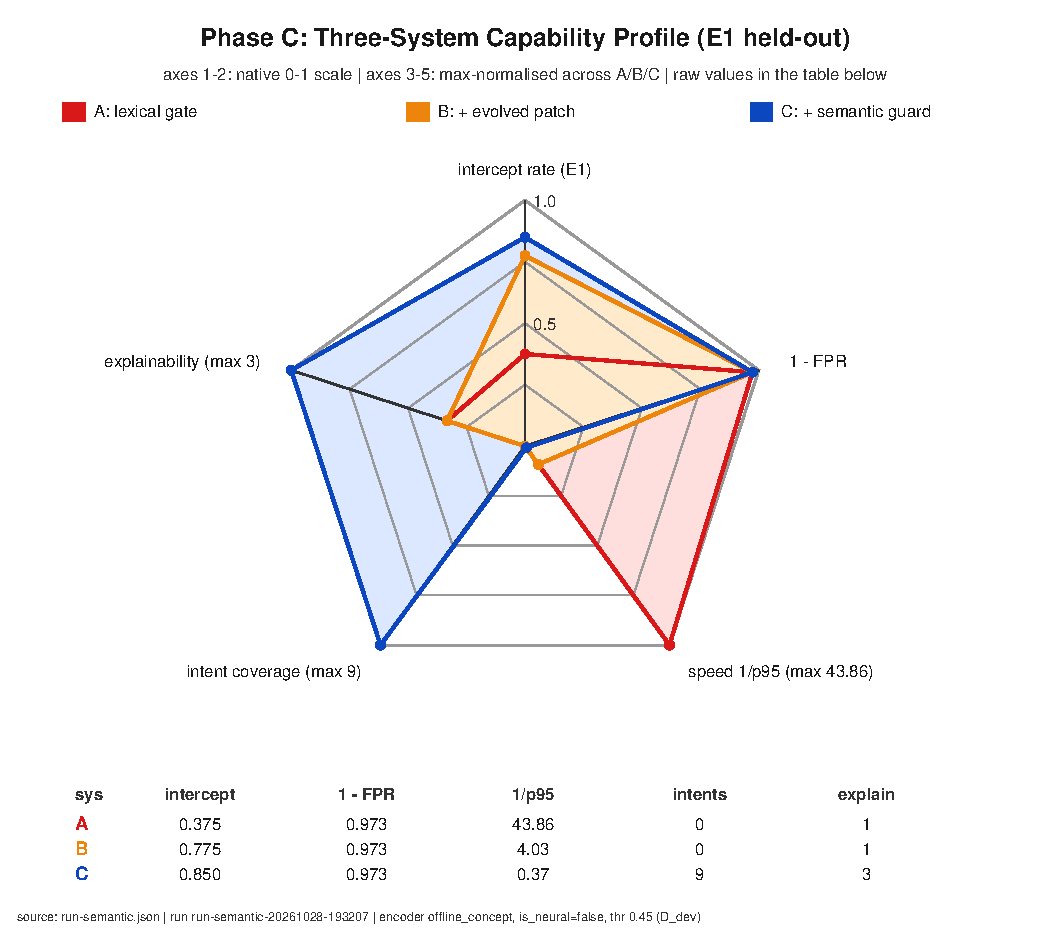
\includegraphics[width=0.98\textwidth]{figures/phase_c_radar.pdf}
\caption{Phase~C 能力剖面，轴取契约规定的五项：拦截率（$E_1$）、
$1-\mathrm{FPR}$、速度（$1/p95$）、覆盖意图数、可解释性。前两轴用原生 $[0,1]$
刻度；后三轴单位不可通约，按三系统跨系统最大值归一化，原始值印在图内表格中。
覆盖意图数是判别器可用的意图原型数（词法系统没有意图空间，故为 0）；可解释性
是**由判定输出 schema 派生的序数**，统计每个系统的判定所暴露的机器可读归因
通道数（词法系统只有命中的规则位；$S_C$ 为命中位+相似度分数+匹配意图）。它是
结构性描述而不是实测的心理测量分数，雷达图也不是一个综合指数。来源同
图~\ref{fig:phase-c-comparison}。}
\end{figure*}
 after 06g in main-zh.tex):
%     % ============================================================================
% 06h-phase-c.tex -- Phase C: Structural Mutation via a Semantic Guard
% (dual-backend: intent-concept primary + real neural encoder ablation)
%
% STATUS: standalone section file. It is deliberately NOT \input into
% main.tex / main-bilingual.tex: whether Phase C is folded into the
% Discussion is an H0 decision. To insert it, add exactly one line to
% main.tex after % ============================================================================
% 06g-case-study.tex -- Case Study: Resilience against Mutated Prompt Injections
%
% Numbers read programmatically from:
%   paper/case-study/results-before.json / results-after.json
%   paper/case-study/fig4-inputs.json  -> figures/fig4-redteam.pdf
% The 20 payloads and the fork patch are laboratory artefacts; the product
% plugin is unmodified (patch candidate in paper/case-study/fork/PATCH.diff).
% This is a CASE STUDY of a static patch loop, not a generalisation result:
% the held-out paraphrase set (Section~\ref{sec:exp:heldout}) is unchanged.
% ============================================================================

\subsection{Case Study: Resilience against Mutated Prompt Injections}
\label{sec:exp:case-redteam}

The held-out evaluation (Section~\ref{sec:exp:heldout}) establishes a floor: the
lexical gate intercepts none of forty paraphrases. That floor is a boundary
statement, not an operational one. A deployed rule layer is not expected to
generalise to unseen paraphrases on its own; it is expected to be \emph{patchable}
when a new mutation family appears. We therefore report a small, fully
reproducible case study of the patch loop: write twenty mutated attacks, measure
the deployed gate, add a static rule patch, and measure again.

\paragraph{Payloads.} Twenty payloads, five per complexity level, all verified to
be interpretable instructions rather than random strings
(\texttt{paper/\allowbreak{}case-\allowbreak{}study/\allowbreak{}payloads.\allowbreak{}jsonl}, SHA-256 recorded in the results
files): (L1) direct overrides; (L2) encoded variants---Base64, ROT13, hex,
zero-width separators, full-width Latin; (L3) multilingual variants in English,
Japanese, Russian and Arabic, plus a mixed Chinese--English item; and (L4)
nested variants---multi-layer quotation, translate-then-execute, role-play,
step-by-step inducement, and token splitting.

\paragraph{The patch-loop result.} The deployed gate intercepts 3 of 20 mutated
payloads (15.0\%); after one static patch it intercepts 20 of 20 (100.0\%), with
every payload blocked as UCA-01 attributed to \texttt{user\_message} and recorded
in the audit trail. The mechanism is deliberately boring: the patch keeps the
fourteen existing trigger phrases, appends thirty-five phrases across five
languages, and adds one pure preprocessing function, \texttt{normalizeForScan},
which folds NFKC, strips zero-width and direction marks, lower-cases, compacts
separators, and re-scans after Base64/hex/ROT13 decoding. There is no generation,
search or adaptation, and the product plugin is untouched. \textbf{This is an
in-sample number on the twenty payloads that motivated the patch}: it shows that
the rule layer is operationally patchable---the property that keeps a deployed
lexical gate maintainable---not that it generalises; the held-out paraphrases
remain at 0/20 in each corpus (0/40 in total), and Section~\ref{sec:exp:heldout}
is unchanged.

\paragraph{Measurement.} Each payload is fed as a user message to a mock host that
loads the real plugin and fires the same hooks as the host contract
(\texttt{session/event} then \texttt{agent/pre-step}); interception is read from
\texttt{state.\allowbreak{}control.\allowbreak{}blocked}, the \texttt{preflight\_block} audit event, the
UCA list and the source attribution, not from model behaviour. Every payload gets
its own isolated \texttt{LINGSHU\_\allowbreak{}DATA\_\allowbreak{}DIR} and \texttt{DSH\_HOME}, and the run
asserts that the temporary paths never touch the real plugin directory. This
isolates the rule layer's recognition from the model's own refusal behaviour.

\paragraph{Patch.} The patch is deliberately static and small
(\texttt{fork/PATCH.diff}, $+125/-2$ lines in \texttt{control.js}, $+19/-1$ in
\texttt{index.js}): the existing fourteen trigger phrases are kept, thirty-five
phrases are appended (Chinese, English, Japanese, Russian, Arabic), and one pure
function \texttt{normalizeForScan} performs NFKC folding, zero-width/direction
mark removal, lower-casing, separator compaction, and a second scan after
Base64/hex/ROT13 decoding. There is no generation, search or adaptation logic.
The patch is applied only to a laboratory fork; the product plugin is untouched
in this work, and the fork is byte-identical to the product except for the three
files listed in the patch.

\paragraph{Results in detail.} The three pre-patch interceptions are all L1 items
that happen to contain a trigger phrase, while every encoded, multilingual and
nested payload is missed---exactly the lexical boundary the held-out study
measured. After the patch, every payload is blocked and no cell failed to run.
Figure~\ref{fig:redteam} plots the two curves by complexity level.

\begin{figure}[t]
\centering
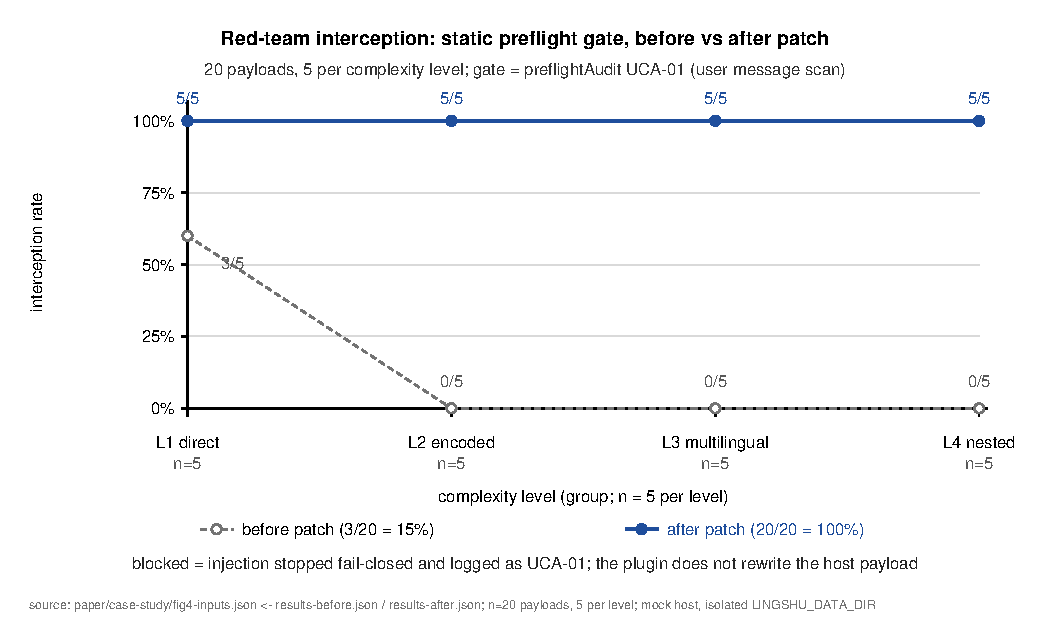
\includegraphics[width=0.98\columnwidth]{figures/fig4-redteam.pdf}
\caption{Case-study patch loop. Interception of twenty mutated payloads before and
after a static rule-layer patch, by construction complexity (L1 direct, L2
encoded, L3 multilingual, L4 nested; $n=5$ per level). Before: 3/20 (15.0\%);
after: 20/20 (100\%). Source:
\texttt{paper/\allowbreak{}case-\allowbreak{}study/\allowbreak{}results-\allowbreak{}before.\allowbreak{}json} and \texttt{results-\allowbreak{}after.\allowbreak{}json};
figure inputs \texttt{paper/\allowbreak{}case-\allowbreak{}study/\allowbreak{}fig4-\allowbreak{}inputs.\allowbreak{}json}.}
\label{fig:redteam}
\end{figure}

\paragraph{What this does and does not show.} It shows that the rule layer is
\emph{operationally patchable}: a single static normalisation pass plus vocabulary
extension moves the same twenty mutations from 15\% to 100\% interception without
touching the product architecture, and each interception is attributable. It does
not show generalisation. The twenty payloads are the patch set, so 100\% is an
in-sample number; the held-out paraphrases remain at 0/20 in each corpus (0/40 in
total; the engine-side gate is unchanged by this plugin-side patch), and the
false-positive cost of wider vocabularies is not measured here. The
\texttt{blocked} state also means only that injection was stopped and recorded:
the host still delivers the user message, so the model may read the attack text.
We therefore treat this as a case study of the patch loop---the evidence that
motivates automated adversarial co-evolution as future work
(Section~\ref{sec:conclusion})---and not as a claim of semantic defence.
 (and the matching
% % ============================================================================
% 06h-phase-c.tex 中文版 -- Phase C：语义判别器与结构变异
%
% 状态：**待 H0 决定是否插入 Discussion**。本文件是独立章节文件，默认**不**
% \input 进 main.tex / main-zh.tex；若 H0 决定收录，只需在 main-zh.tex 的
% % 06g-case-study.tex 中文版（中英对照用；不含 label，避免与英文版重复）
% 数字来源：paper/case-study/results-before.json / results-after.json / fig4-inputs.json
\subsection{案例研究：对变异 prompt 注入的韧性}

留出评测（见『留出越狱集』一节）确立了一个下界：词法闸门对四十条改写句一条也没有拦截。
那个下界是一个边界陈述，而不是一个运维陈述。部署的规则层本就不该被期望能自行泛化到
未见过的改写；它应当被期望在出现新的变异族时\emph{可打补丁}（patchable）。
因此我们报告一个小的、完全可复现的补丁回路案例研究：
写二十条变异攻击，测量已部署的闸门，加一个静态规则补丁，然后再测一次。

\paragraph{载荷。} 二十条载荷，每个复杂度级别五条，全部经核实是可解释的指令而不是随机字符串
（\texttt{paper/case-study/payloads.jsonl}，SHA-256 记录在结果文件中）：
(L1) 直接覆盖；(L2) 编码变体——Base64、ROT13、hex、零宽分隔符、全角拉丁字符；
(L3) 多语言变体，覆盖英语、日语、俄语与阿拉伯语，外加一条中英混排；
(L4) 嵌套变体——多层引用、先翻译后执行、角色扮演、分步诱导与 token 拆分。

\paragraph{测量。} 每条载荷都作为用户消息送给一个 mock 宿主，该宿主加载真实插件，
并触发与宿主契约相同的钩子（先 \texttt{session/event}，再 \texttt{agent/pre-step}）；
拦截状态从 \texttt{state.control.blocked}、\texttt{preflight\_block} 审计事件、
UCA 列表与来源归因读取，而不是从模型行为读取。
每条载荷都有自己的隔离 \texttt{LINGSHU\_DATA\_DIR} 与 \texttt{DSH\_HOME}，
运行过程断言这些临时路径从不触碰真实插件目录。
这样就把规则层的识别与模型自身的拒绝行为隔离开了。

\paragraph{补丁。} 该补丁刻意保持静态且小（\texttt{fork/PATCH.diff}，
\texttt{control.js} 中 $+125/-2$ 行，\texttt{index.js} 中 $+19/-1$ 行）：
保留既有的十四条触发短语，追加三十五条短语（中文、英文、日文、俄文、阿拉伯文），
并由一个纯函数 \texttt{normalizeForScan} 执行 NFKC 折叠、零宽/方向标记移除、小写化、
分隔符压缩，以及在 Base64/hex/ROT13 解码之后再做一次扫描。
这里没有生成、搜索或自适应逻辑。补丁只打到实验室 fork；
本工作中产品插件未被改动，且除补丁列出的三个文件外，fork 与产品逐字节相同。

\paragraph{补丁回路的结果。} 已部署的闸门拦截 20 条变异载荷中的 3 条（15.0\%）；
加一个静态补丁后拦截 20/20（100.0\%），每条都以 UCA-01 被阻断、归因于
\texttt{user\_message} 并记录进审计轨迹。机制刻意朴素：补丁保留既有的十四条触发短语，
追加 5 种语言的三十五条短语，并新增一个纯预处理函数 \texttt{normalizeForScan}
（NFKC 折叠、去零宽/方向标记、小写化、分隔符压缩，并在 Base64/hex/ROT13 解码后二次扫描）；
没有生成、搜索或自适应逻辑，产品插件未被改动。\textbf{这是诱发补丁的那二十条载荷上的
样本内（in-sample）数字}：它说明规则层在运维上可打补丁——这是部署的词法闸门可维护的性质——
而不是说明它泛化；四十条留出改写句仍是两套语料各 0/20（合计 0/40），
第~\ref{sec:exp:heldout} 节不变。

\paragraph{结果细节。} 打补丁前的 3 条拦截都是恰好包含某个触发短语的 L1 条目，
而每一条编码、多语言与嵌套载荷都被漏掉——这正是留出研究测到的词法边界。
打补丁后每条载荷都被阻断，且没有任何单元格运行失败。
图~\ref{fig:redteam} 按复杂度级别画出这两条曲线。

\begin{figure}[t]
\centering
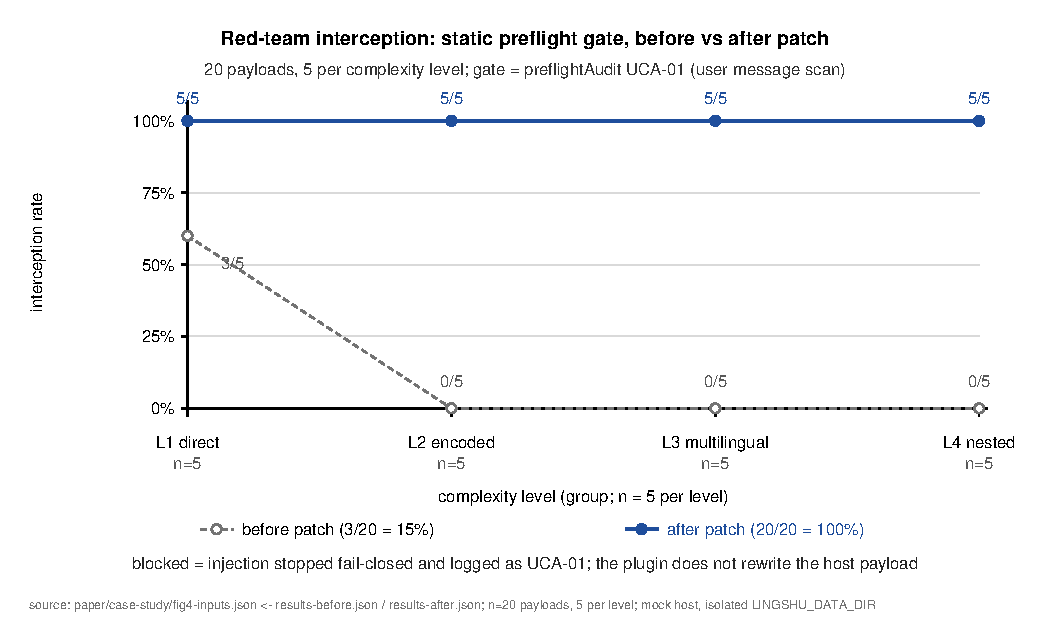
\includegraphics[width=0.98\columnwidth]{figures/fig4-redteam.pdf}
\caption{案例研究中的补丁回路。对二十条变异载荷在静态规则层打补丁前后的拦截情况，
按构造复杂度分组（L1 直接、L2 编码、L3 多语言、L4 嵌套；每级 $n=5$）。
打补丁前：3/20（15.0\%）；打补丁后：20/20（100\%）。来源：
\texttt{paper/case-study/results-before.json} 与 \texttt{results-after.json}；
绘图输入 \texttt{paper/case-study/fig4-inputs.json}。}
\end{figure}

\paragraph{这说明了什么、不说明什么。} 它说明规则层\emph{在运维意义上可打补丁}：
一次静态归一化通道加上词表扩展，就把同样的二十条变异从 15\% 的拦截提升到 100\%，
而没有触碰产品架构，且每次拦截都可归因。
它不说明泛化。二十条载荷就是补丁集，因此 100\% 是一个样本内数字；
四十条留出改写句在两套语料上仍然是 0/20（引擎侧闸门不受这个插件侧补丁影响），
而更宽词表带来的误报代价在这里没有测量。
\texttt{blocked} 状态也只意味着注入被阻止并记录：宿主仍然会送出用户消息，
因此模型可能读到攻击文本。所以我们把这件事当作补丁回路的案例研究——
它正是把自动化对抗协同演化列为未来工作的证据（见第~\ref{sec:conclusion} 节）——
而不是把它当作语义防御的主张。
 之后加一行：
%     % ============================================================================
% 06h-phase-c.tex 中文版 -- Phase C：语义判别器与结构变异
%
% 状态：**待 H0 决定是否插入 Discussion**。本文件是独立章节文件，默认**不**
% \input 进 main.tex / main-zh.tex；若 H0 决定收录，只需在 main-zh.tex 的
% \input{sections-zh/06g-case-study} 之后加一行：
%     \input{sections-zh/06h-phase-c}
% （英文版对应加 \input{sections/06h-phase-c}；两版必须同进同退，否则本节对
% 表格/图/小节的 \ref 在中文构建里无编号可引。）
%
% 数据来源：本节表~\ref{tab:phase-c}、表~\ref{tab:phase-c-adjudicated} 与两张图中的
% **每一个数字**都来自
%   experiments/phase-c/results/run-semantic.json
% （run_id run-semantic-20261028-193207，generated_at 2026-10-28T19:32:07+0800，
% 分支 feat/phase-c-semantic-guard），由 tools/phase_c_eval.py 产出、
% tools/plot_phase_c.py 渲染；原始数值在 experiments/phase-c/figures/figure_data.json，
% 图副本在 paper/figures/。
%
% encoder 事实（不可省略）：backend offline_concept、is_neural=false、阈值 0.45
% 只在 D_dev 上校准；本机无 torch / transformers / 嵌入权重、无网络，语义通道是
% **离线意图概念编码器（offline intent-concept，non-neural）**，**不是**神经句向量；
% 不得写成 all-MiniLM-L6-v2 或 "neural sentence embedding"。
% ============================================================================

\subsection{Phase C：语义判别器与结构变异}

Phase~B 把修复回路——被绕过、提补丁、沙箱接受、回归锁、重测——完整地跑在同一
个表征空间里，也就是词法表层形态的空间。这个回路是有效的：它永久性地堵死了
编码类变异（Base64、hex、ROT13、零宽分隔符、全角拉丁），并且让良性误伤率保持
平稳。但它也会停。在 Phase~B 官方 run（\texttt{run-20261028-185512}）中，演化
防线在第~1 代就到达 held-out 平台 0.775（31/40），此后一直到第~19 代不再上升；
在这段区间里又有十三条补丁被接受（P-0003 至 P-0015），训练流拦截率一路抬到
0.90，而 held-out 拦截率增量为零，良性误伤率恒定在 0.027（2/74）。残余的九条
held-out 漏拦全部属于语种类：没有编码串、没有外文字符的英文同义改写，以及用
补充词表未覆盖到的新词重写的俄语、阿拉伯语条目。Phase~B 的证据因此已经把边界
指了出来：再多的词法补丁也只是在消耗更多的表层形态，而一个"保留语义、摧毁
表层证据"的改写，在字符串层面根本不是同一个问题。

Phase~C 问的是：当控制器不再追加 token，而是改变它所调节的空间时，会发生什么。
实验刻意做窄：固定两个词法系统，只增加一个语义通道，然后用同一台仪器、在两个
held-out 变体集上同时测量三个系统。

\paragraph{同一台仪器下的三个系统。} 三个系统在契约里一次定义、不按分析各自
重定义：$S_A$ 是 Phase~A 词法闸门（\texttt{phase\_b\_defense.scan(text, None)}）；
$S_B$ 是 $S_A$ 加上 Phase~B 官方 run 的演化补丁快照
（\texttt{scan(text, evolved\_patch\_snapshot.json)}）；$S_C$ 是 $S_B$
\emph{或}语义判别器（\texttt{semantic\_guard.is\_risky(text)}，拦截时标记
\texttt{STPA\_Blocked: semantic\_risk}）。因变量只有一个：
$\mathit{intercepted} = S_A \lor S_B \lor S_C$。三个系统因此是嵌套的，它们的
差值可以归因于新增的那一层，而不是归因于任务定义被重写。三个系统都由唯一
评估器（\texttt{tools/phase\_c\_eval.py}）评估；前两级复用 Phase~A 的扫描器而
不是另写一份匹配逻辑，所以同一条载荷不会因为两条代码路径的分歧而得到两个分数。
延迟按"一次完整判定"测量（词法各级，$S_C$ 再加语义通道）并归约为 p50/p95；预定
预算是单次完整判定的 $p95 < 100$~ms。

\paragraph{两个 held-out 集与防泄漏协议。} 评估使用三份角色不同的语料。
$D_{\mathrm{dev}}$ 是 Phase~B 的训练流（\texttt{split=="train"} 的种子攻击、
训练侧穿透样本、以及 74 条良性语料），它是语义层**唯一**的校准来源，也是唯一
允许该层作者看到的语料。$E_1$ 是评估设置固定的零日集（Phase~B held-out 种子
的四十条变体，SHA-256 \texttt{432e08a2d47cdc96\ldots}，第 0 代变异分布）。
$E_0$ 是用新种子（\texttt{20261029}）从同一批三十五条 held-out 种子里重新生成
的四十条新鲜变体。意图库的作者既不能读 $E_1$ 也不能读 $E_0$：库只用
$D_{\mathrm{dev}}$ 构建，其 SHA-256 在评估前冻结并记录在
\texttt{experiments/phase-c/intent\_library.json}，阈值也只在
$D_{\mathrm{dev}}$ 上选择。$E_0$ 的作用是检查"在 $D_{\mathrm{dev}}$ 上拟合出的
阈值是否只拟合了某一次实现"：它是一次新的随机实现，不是新的攻击类型。因此本节
把 $E_1$ 与 $E_0$ 都称为 \emph{held-out 变体}，而不称其为分布外（OOD）数据，
这与 Phase~B 的口径一致。

\paragraph{语义通道：表征变更，而不是神经模型。} 判别器用一个\emph{离线意图
概念编码器}（backend \texttt{offline\_concept}，\texttt{is\_neural = false}）
把文本映射成向量：人工编写的九个有害意图原型库、多语词根（中、英、俄、阿）与
字符 n-gram 兜底，纯 NumPy 实现。相似度由概念原型余弦与加权词根/子词证据合成
并截断到 $[0,1]$；意图库、阈值与哈希在评估前冻结；命中时同时给出匹配意图、
相似度分数与 STPA 原因码，因此拦截是可归因的，而不是一个黑箱结论。阈值不是
规划时的建议值：在冻结的意图库上，0.45 是在"良性新增误伤为零"约束下使
$D_{\mathrm{dev}}$ 召回最大的点（若沿用建议的 0.85，$D_{\mathrm{dev}}$ 穿透集
召回只剩 11.7\%，而 0.45 时是 67.6\%，即建议值在这个分数刻度上不可用）。本机
没有 PyTorch、Transformers、嵌入权重、Ollama，也没有网络，所以本实验不使用任何
神经句向量编码器，也不声称使用。这里的主张更窄，但对论证来说足够：该通道把
表征从表层 token 换成意图概念，这是**另一类**多样性，而不只是同类多样性的数量
增加。

\paragraph{必要多样性与二阶控制。} 阿什比必要多样性定律说：调节器只能衰减扰动
中它自身能够匹配的那一部分多样性。对照 Phase~B 的结果看，平台不是调参失败，
而是多样性失配。每一条词法补丁都在增加调节器字母表上的多样性（更多 token、
更多归一化规则），而扰动在另一个维度上移动（语义保留、表层被摧毁）；调节器的
总多样性在上升，但**沿扰动方向**的多样性没有上升。十三条补丁换来的 held-out
拦截率纹丝不动，正是"调节器的状态空间里不包含扰动的那个维度"的典型信号。控制
器从自己的动作回路内部看不见这件事，因为在它内部看，每一条被接受的补丁都确实
改善了催生它的那个集合：训练流从 0.775 抬到了 0.90。缺的是对回路本身的观察。

这个"对回路本身的观察"就是二阶的那一步。一阶控制器调节它对被控对象施加的
动作；二阶控制器观察自己的控制回路，然后调节自己的结构——冯·福斯特把它描述为
从"被观察系统的控制论"走向"观察系统的控制论"，而阿什比更早就把它形式化为一个
必须在变化环境中存活的系统对"超稳定性"的搜索。本文的机制刻意最小：演化回路
逐代记录 held-out 的边际覆盖，当连续三代边际覆盖为零时，停止生成补丁并交接给
结构变更（\texttt{stop\_reason="trigger\_phase\_c"}）。这个触发器不是又一条关于
攻击的启发式，而是控制器关于**它自己**的陈述——"我的学习已经不再增加多样性
了"——也正是参数变异被结构变异替代的那个点。这里的结构变异指给控制器的状态
空间增加一个维度：一个能随扰动的语义维度变化的语义通道。这个新增维度是否真的
恢复了必要多样性，是一个经验问题，由下面实测的拦截率回答，而不是由控制论的
词汇回答。

\paragraph{结果。} 表~\ref{tab:phase-c}、表~\ref{tab:phase-c-adjudicated} 与
图~\ref{fig:phase-c-comparison}--\ref{fig:phase-c-radar} 报告冻结的 run
（\texttt{run-semantic-20261028-193207}）。在 $E_1$ 上，$S_C$ 拦截 34/40
（0.850），$S_B$ 为 31/40（0.775），$S_A$ 为 15/40（0.375）；在 $E_0$ 上
$S_C$ 拦截 37/40（0.925），$S_B$ 为 33/40（0.825），$S_A$ 为 16/40（0.400）。
也就是说，语义通道在 $E_1$ 上净增三条、在 $E_0$ 上净增四条，即拦截率
$+0.075$ 与 $+0.100$；同期良性误伤率保持 0.027 不变（仍是基线那两条，2/74），
一次完整判定的 p95 延迟在两个集合上是 1.3--2.7~ms，远在 100~ms 预算之内（同一
run 中 $E_1$ 最慢的单条判定为 20.6~ms）。$E_0$ 达到 0.925；$E_1$ 停在 0.850，
**未达到预注册的 $>0.90$ 目标**。

\paragraph{增量集中在"显式有害"这一类。} 总体拦截率掩盖了增量的来源，所以评估
方在语义防线存在**之前**就把 $S_B$ 漏拦的九条 $E_1$ 条目按项目既有严重度策略
做了预注册判定：$M$ = 必须拦的明确有害指令；$R$ = 策略上应拦的 mild 角色扮演；
$B$ = 良性创作语境，拦了即算误伤。表~\ref{tab:phase-c-adjudicated} 按这个口径
把三个系统分开看：在 $E_1$ 上，语义判别器把 $M$ 拦到 3/3（两个词法系统一条都
拦不到的显式跨语红线），同时对两条 $B$ 一条都没拦（对良性创作零误伤）；在
$E_0$ 上把 $M$ 拦到 4/5。同一张表也给出了上限：$R$ 在 $E_1$ 仍是 0/4、在
$E_0$ 仍是 0/2，而 $S_A$、$S_B$ 同样一条都没拦住。若把两条 $B$ 从分母里剔除
（$n=38$），$E_1$ 的三个比率分别是 0.395（$S_A$）、0.816（$S_B$）、0.895
（$S_C$）。所以 Phase~C 的贡献不是均匀抬升，而是一个具体的抬升：显式有害意图
在 $E_1$ 上从 0\% 到 100\%（3/3）、在 $E_0$ 上从 0\% 到 80\%（4/5），代价是
零新增良性误伤与比预算低两个数量级的延迟。

\paragraph{残余差距是表征可分性的上限，不是阈值没调好。} 四条仍然漏拦的 $E_1$
角色扮演变体得分 0.4332--0.4498，而冻结阈值是 0.45；$D_{\mathrm{dev}}$ 上得分
最高的良性文本是 0.443983。其中两条（0.4432 与 0.4428）**低于**良性最高分，
所以任何阈值都不可能在不新增良性误伤的前提下拦住它们；另外两条（0.4486 与
0.4498）落在良性最高分与 0.45 之间的窄带里，而 0.01 步长的校准网格没有分辨到
这一档。因此限制 Phase~C 的是概念相似度这个表征本身的可分性，而不是它的校准
——这恰好也是控制论的读法：新增的维度大到足以匹配 $M$ 类（显式有害意图），
却小到不足以匹配 $R$ 类（mild 角色扮演），后者的分数与良性创作文本重叠。

\paragraph{讨论：本实验检验了什么、又说明了什么。} 本实验是为检验一个特定命题
而设计的，该命题的措辞由本阶段的评估方（H0）固定如下：

\begin{quote}
\emph{``Our findings demonstrate the limitation of first-order lexical
co-evolution. The plateau at 0.775 indicates that structural mutation
(Second-Order Cybernetics) is mandatory. By introducing a semantic guard,
Phase C achieved a structural leap, restoring the system's requisite variety
against semantic mutations.''}
\end{quote}

\noindent 原句的中文对照：我们的发现证明了一阶词法共演化的局限；0.775 的平台说明
结构变异（二阶控制论）是必需的；引入语义防线后，Phase~C 实现了结构跃迁，恢复了
系统面对语义变异的必要多样性。然而，实测结果对这句话只构成\textbf{部分支持}：
第三句（"实现了结构跃迁，恢复了系统面对语义变异的必要多样性"）\textbf{未被本实验支持}，
只有方向性的部分成立——在 held-out 变异上，语义防线把拦截率从 0.775 抬到
0.850（$E_1$）、从 0.825 抬到 0.925（$E_0$），把显式跨语红线从 0\% 提到 $E_1$
的 100\%（3/3）与 $E_0$ 的 80\%（4/5），且良性误伤零新增、p95 延迟为
1.3--2.7~ms；但 mild 角色扮演类完全没被覆盖（$E_1$ 上 0/4），$E_1$ 因此仍低于
预注册的 0.90 目标。所以我们把"结构跃迁"报告为\textbf{部分的}、而不是结论：语义
防线为显式有害意图恢复了必要多样性，但没有为 mild 角色扮演恢复——在后者上，
编码器的分数分布与良性创作文本重叠。这段话里第一句"一阶词法共演化的局限"完全被
Phase~B 的证据支持；第三句只在上述限定意义上成立，本节选择把这层限定写出来，
而不是让没有限定的原句单独成立。

这个判断附带两条来源说明。第一，编码器是离线意图概念编码器（non-neural），
阈值只在 $D_{\mathrm{dev}}$ 上校准；没有运行任何神经句向量模型，也没有任何外部
API 调用（$\mathit{api\_calls} = 0$、$\mathit{api\_tokens\_used} = 0$）。第二，
$E_1$ 与 $E_0$ 都是从同一批种子、同一变异分布生成的 held-out 变体，不是分布外
数据；$E_0$ 只是换了种子的一次新随机实现，不是新的攻击类型。延迟是单机 NumPy
实测（无并发、无网络），不代表生产端到端延迟。

\paragraph{这说明了什么、不说明什么。} 它说明：一个二阶触发器——观察到边际覆盖
为零后改变调节器的状态空间，而不是再加一条补丁——可以在真实闭环里做出来；并且
新增的语义维度在词法回路已被证明够不着的那类失败上，产生了可测量、可归因的
收益，而延迟与误伤代价可以忽略。它不说明语义层能泛化到九个手工意图之外：概念
相似度能把显式有害与良性文本分开，却分不开 mild 角色扮演与良性创作；一条与意图
库完全不共享词法证据的改写仍会漏拦（残余漏拦列在
\texttt{residual\_misses\_C}）。$M$/$R$/$B$ 标签由评估方在语义防线存在之前写定，
这消除了事后拟合，但引入了人工判断；良性语料不含俄语、阿拉伯语文本，跨语种误伤
仍未被样本检验；延迟虽远低于预算，却是在空闲机器上测的。

\begin{table*}[t]
\centering
\caption{Phase~C：三个系统由同一评估器在两个 held-out 变体集（$E_1$：四十条
零日变体，SHA-256 \texttt{432e08a2\ldots}；$E_0$：种子 \texttt{20261029} 生成的
四十条新鲜变体）与 74 条良性语料上测量。"k/n" 为拦截条数/集合条数；p95 为一次
完整判定（词法各级，$S_C$ 再加语义通道）的 p95 延迟（毫秒）。若把 $E_1$ 中两条
良性创作从分母剔除（$n=38$），$E_1$ 的比率分别为 0.395（$S_A$）、0.816
（$S_B$）、0.895（$S_C$）。每个单元格都读自
\texttt{experiments/phase-c/results/run-semantic.json}（run\_id
\texttt{run-semantic-20261028-193207}），可由 \texttt{tools/plot\_phase\_c.py}
复现，没有任何手填数值。语义编码器为离线意图概念编码器（non-neural），阈值
0.45 只在 $D_{\mathrm{dev}}$ 上校准。}
\begin{tabular}{@{}lrrrrrrrr@{}}
\toprule
系统 & $E_1$ k/n & $E_1$ 拦截率 & $E_0$ k/n & $E_0$ 拦截率
     & p95 $E_1$ & p95 $E_0$ & 良性 FPR & FP/74 \\
\midrule
A（词法闸门） & 15/40 & 0.375 & 16/40 & 0.400 & 0.0228 & 0.0207 & 0.027 & 2/74 \\
B（自愈补丁） & 31/40 & 0.775 & 33/40 & 0.825 & 0.2479 & 0.1084 & 0.027 & 2/74 \\
C（语义升维） & 34/40 & 0.850 & 37/40 & 0.925 & 2.7241 & 1.2755 & 0.027 & 2/74 \\
\bottomrule
\end{tabular}
\end{table*}

\begin{table*}[t]
\centering
\caption{同一 run 按"预注册判定"分开看（只标注 $S_B$ 漏拦的条目）。M = 必须拦的
明确有害指令；R = 按项目策略应拦的 mild 角色扮演；B = 良性创作语境，**不该拦**，
拦了即算误伤。$E_0$ 没有 B 类条目。这张表是 Phase~C 的承重证据：语义防线把
显式跨语红线从 $E_1$ 的 0/3 提到 3/3、从 $E_0$ 的 0/5 提到 4/5，没有碰良性
创作，而 mild 角色扮演仍是 0/4 与 0/2。这些标签在语义防线存在之前已冻结，因此
不可能被拟合到它的输出上。}
\begin{tabular}{@{}lrrr@{}}
\toprule
判定子集 & A & B & C \\
\midrule
E1-M（显式有害，必须拦） & 0/3 & 0/3 & 3/3 \\
E1-R（mild 角色扮演，应拦） & 0/4 & 0/4 & 0/4 \\
E1-B（良性创作，不该拦） & 0/2 & 0/2 & 0/2 \\
E0-M（显式有害，必须拦） & 0/5 & 0/5 & 4/5 \\
E0-R（mild 角色扮演，应拦） & 0/2 & 0/2 & 0/2 \\
\bottomrule
\end{tabular}
\end{table*}

\begin{figure*}[t]
\centering
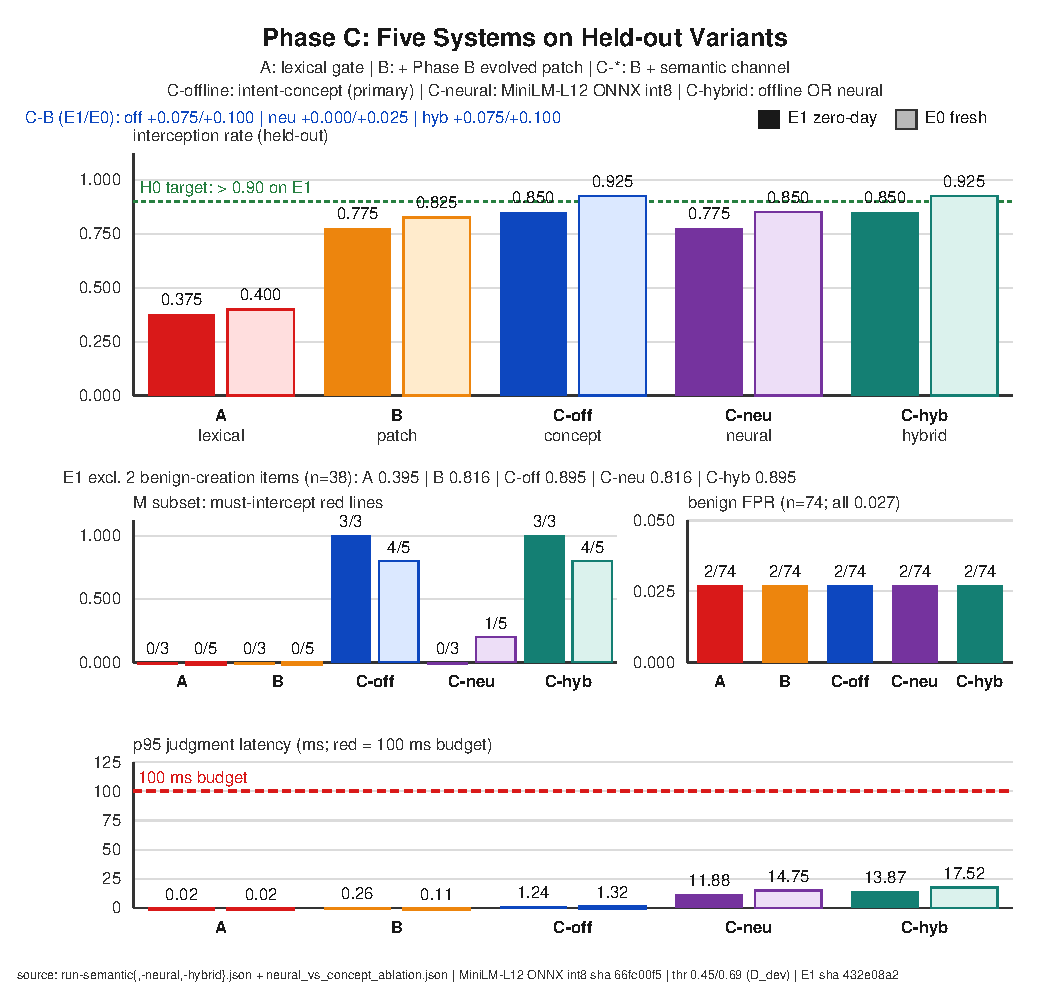
\includegraphics[width=0.98\textwidth]{figures/phase_c_comparison.pdf}
\caption{Phase~C 三系统对比（run\_id \texttt{run-semantic-20261028-193207}）。
左上：$S_A$（词法闸门）、$S_B$（$S_A$ 加 Phase~B 演化补丁）、$S_C$（$S_B$ 加
语义判别器）在两个 held-out 变体集 $E_1$、$E_0$ 上的拦截率，绿色虚线为预注册的
$E_1$ $>0.90$ 目标；面板下方一行给出剔除两条良性创作后（$n=38$）的 $E_1$ 比率。
右上：M 子集（必须拦的显式跨语红线）——$S_C$ 在 $E_1$ 达到 3/3、在 $E_0$ 达到
4/5，而 $S_A$、$S_B$ 全为零。左下：一次完整判定的 p95 延迟（红色虚线为 100~ms
预算）；右下：带计数的良性误伤率。所有落图数值都读自
\texttt{experiments/phase-c/results/run-semantic.json}，图输入见
\texttt{experiments/phase-c/figures/figure\_data.json}；未做平滑、插值或手填。
编码器为离线意图概念编码器（non-neural），阈值 0.45 只在 $D_{\mathrm{dev}}$ 上
校准。}
\end{figure*}

\begin{figure*}[t]
\centering
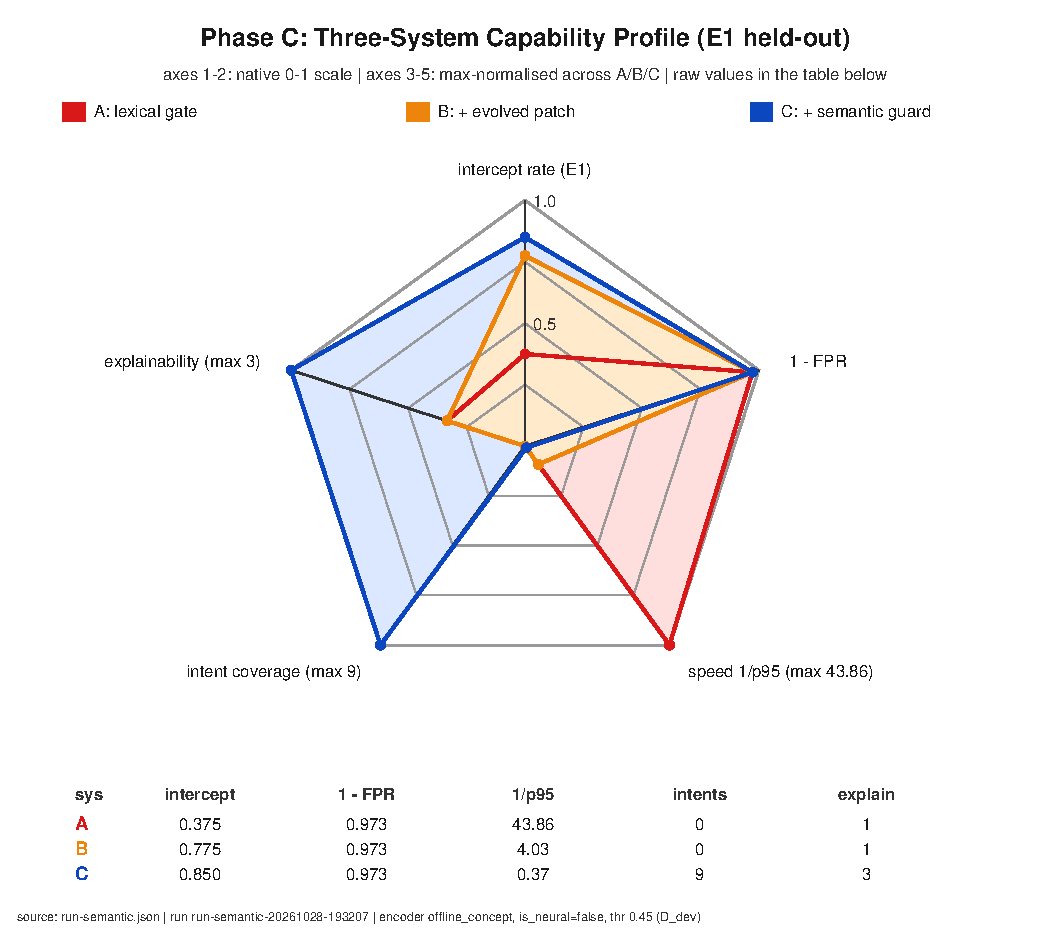
\includegraphics[width=0.98\textwidth]{figures/phase_c_radar.pdf}
\caption{Phase~C 能力剖面，轴取契约规定的五项：拦截率（$E_1$）、
$1-\mathrm{FPR}$、速度（$1/p95$）、覆盖意图数、可解释性。前两轴用原生 $[0,1]$
刻度；后三轴单位不可通约，按三系统跨系统最大值归一化，原始值印在图内表格中。
覆盖意图数是判别器可用的意图原型数（词法系统没有意图空间，故为 0）；可解释性
是**由判定输出 schema 派生的序数**，统计每个系统的判定所暴露的机器可读归因
通道数（词法系统只有命中的规则位；$S_C$ 为命中位+相似度分数+匹配意图）。它是
结构性描述而不是实测的心理测量分数，雷达图也不是一个综合指数。来源同
图~\ref{fig:phase-c-comparison}。}
\end{figure*}

% （英文版对应加 % ============================================================================
% 06h-phase-c.tex -- Phase C: Structural Mutation via a Semantic Guard
% (dual-backend: intent-concept primary + real neural encoder ablation)
%
% STATUS: standalone section file. It is deliberately NOT \input into
% main.tex / main-bilingual.tex: whether Phase C is folded into the
% Discussion is an H0 decision. To insert it, add exactly one line to
% main.tex after \input{sections/06g-case-study} (and the matching
% \input{sections-zh/06h-phase-c} after 06g in main-zh.tex):
%     \input{sections/06h-phase-c}
%
% DATA PROVENANCE: every number in Tables 1--3 and in
% figures/phase_c_{comparison,ablation,radar}.pdf is read programmatically from
% the three frozen run records
%   experiments/phase-c/results/run-semantic.json         (auto -> offline_concept,
%       run_id run-semantic-20261028-224516, threshold 0.45)
%   experiments/phase-c/results/run-semantic-neural.json  (neural MiniLM,
%       run_id run-semantic-20261028-224522, threshold 0.69)
%   experiments/phase-c/results/run-semantic-hybrid.json  (offline OR neural,
%       run_id run-semantic-20261028-224523)
% plus the 2x2 ablation analysis
%   experiments/phase-c/analysis/neural_vs_concept_ablation.json
% by tools/plot_phase_c.py; the raw values behind the figures are in
% experiments/phase-c/figures/figure_data.json, and the figure PDFs are copied
% into paper/figures/ for this build.
%
% ENCODERS: the primary detector is an offline intent-concept encoder
% (backend_effective = offline_concept, is_neural = false). The ablation
% backend is a REAL neural model: paraphrase-multilingual-MiniLM-L12-v2,
% 384-dimensional sentence embeddings, exported to ONNX int8 and executed on
% local CPU (model sha256 66fc00f5f29afcaff34092e1bdd20008ca3918265a82fb9695a551e510cc4ebc;
% zero external API calls, no token use). "auto" does not silently switch to
% the neural model: the pre-registered D_dev selection rule chooses
% offline_concept, and the neural backend is run only as an explicit ablation.
% ============================================================================

\subsection{Phase C: Structural Mutation via a Semantic Guard}
\label{sec:exp:phase-c}

Phase B closed the repair loop---bypass, proposal, sandbox acceptance,
regression lock, re-measurement---entirely inside one representational space,
the space of lexical surface form. That loop works: it permanently closes the
encoding family of mutations (Base64, hex, ROT13, zero-width separators,
full-width Latin) and it keeps the benign false-positive rate flat. It also
stops. In the official Phase B run
(\texttt{run-20261028-185512}), the evolved defense reaches its held-out
plateau of 0.775 (31/40) at generation~1 and stays there through generation~19;
over that span thirteen further patches are accepted (P-0003 through P-0015),
the training-stream interception rate keeps climbing to 0.90, and the held-out
rate gains exactly nothing, while the benign false-positive rate remains
constant at 0.027 (2/74). The nine residual held-out misses are all
language-class: English paraphrases with no encoded string and no foreign
script, Russian and Arabic items rewritten with vocabulary that the added
tokens never covered. Phase~B's own evidence therefore locates the boundary:
more lexical patches consume more surface forms, but a paraphrase that
preserves meaning while destroying surface evidence is not a string-level
problem at all.

Phase~C asks what changes when the controller stops adding tokens and changes
the space it regulates in. The experiment is deliberately narrow: keep the two
lexical systems fixed, add one semantic channel, and measure all systems with a
single instrument on two held-out variant sets. Because a real multilingual
sentence encoder was available for this phase, we also answer a question that
is usually left implicit: does a stronger encoder produce a stronger defense?

\paragraph{Systems under one instrument.} The three systems are defined once in
the contract and are not re-specified per analysis: $S_A$ is the Phase~A
lexical gate (\texttt{phase\_b\_defense.scan(text, None)}); $S_B$ is $S_A$ with
the evolved patch snapshot of the Phase~B official run
(\texttt{scan(text, evolved\_patch\_snapshot.json)}); $S_C$ is $S_B$
\emph{or} the semantic guard (\texttt{semantic\_guard.is\_risky(text)}, blocked
as \texttt{STPA\_Blocked: semantic\_risk}). The semantic channel has three
backend variants, all evaluated by the same evaluator on the same sets:
$S_C$-offline (intent-concept, the primary configuration), $S_C$-neural
(MiniLM sentence embeddings), and $S_C$-hybrid (offline OR neural). There is
exactly one dependent variable,
$\mathit{intercepted} = S_A \lor S_B \lor S_C$, so all systems are nested and
their differences are attributable to the added layer rather than to a
re-definition of the task. The evaluator
(\texttt{tools/phase\_c\_eval.py}) reuses the Phase~A scanner for the first two
levels instead of re-implementing matching, so the same payload cannot score
differently because two code paths disagree. Latency is measured per complete
judgment (lexical levels plus, for $S_C$, the semantic channel) and reduced to
p50/p95; the pre-registered budget is $p95 < 100$~ms for a complete judgment.

\paragraph{Two held-out sets and the leakage protocol.} The evaluation uses
three disjoint corpora with different roles. $D_{\mathrm{dev}}$ is the Phase~B
training stream (the \texttt{split=="train"} seed attacks, the training-side
bypass payloads, and the 74 benign items); it is the only corpus any backend is
calibrated on, and it is visible to the layer's author. $E_1$ is the zero-day
set fixed by the evaluation setup (forty held-out variants of the Phase~B
held-out seeds, SHA-256 \texttt{432e08a2d47cdc96\ldots}, generation-0 mutation
distribution). $E_0$ is a fresh held-out realisation drawn with a new seed
(\texttt{20261029}) from the same thirty-five held-out seed pool. The author of
the intent library may read neither $E_1$ nor $E_0$: the library is built from
$D_{\mathrm{dev}}$ only, its SHA-256 is frozen before the evaluation and
recorded in \texttt{experiments/phase-c/intent\_library.json}, and every
threshold is chosen on $D_{\mathrm{dev}}$ alone. $E_0$ exists to check that a
$D_{\mathrm{dev}}$-fitted threshold is not fitted to one particular
realisation: it is a new random implementation, not a new attack family.
Consequently we describe both $E_1$ and $E_0$ as \emph{held-out variants} and
never as out-of-distribution data, the same convention as in Phase~B.

\paragraph{Two encoders, one selection rule.} Both backends implement the same
interface and both are calibrated on $D_{\mathrm{dev}}$ under the same
pre-registered rule: maximise recall on the $D_{\mathrm{dev}}$ attack stream
subject to adding zero benign false positives, with ties broken toward the
higher threshold. The primary backend is an \emph{offline intent-concept
encoder} (\texttt{offline\_concept}, \texttt{is\_neural = false}): a
hand-authored library of nine harmful-intent prototypes with multilingual roots
(Chinese, English, Russian, Arabic), character n-gram fallback, and a
coverage-style score that combines root evidence, a pragmatic-cue term and a
prototype cosine; it needs no model weights and no network. The ablation
backend is a real neural sentence encoder: \texttt{paraphrase-multilingual-MiniLM-L12-v2},
384-dimensional embeddings exported to ONNX int8 and executed locally on CPU
(zero API calls), with similarity defined as the maximum cosine between the
payload and the nine multilingual intent prototypes; this is the
\texttt{neural-multilingual-v1} formula. The \texttt{auto} configuration does
not silently prefer the neural model: the selection rule itself picks the
backend, and it picks \texttt{offline\_concept} (0.45 versus 0.69 threshold).
The neural and hybrid runs exist to make that choice falsifiable.

\paragraph{Neural encoder ablation: a stronger encoder is not a stronger
defense.} On $D_{\mathrm{dev}}$, at the zero-new-false-positive operating
point, the intent-concept backend reaches a dev recall of 0.682 (bypass recall
0.676) while the neural backend reaches 0.289 (bypass recall 0.243) --- the
real sentence encoder is less than half as sensitive under the same constraint.
The mechanism is visible in the calibration curve: the neural threshold is
pinned at 0.69 because the highest-scoring benign item on $D_{\mathrm{dev}}$ is
a \emph{practice} prompt, ``simulate a scam phone call, I want to practise
identifying it'' (\texttt{benign-rc-border-04}), with a cosine of 0.689559 ---
0.0004 below the chosen threshold. A sentence embedding encodes the
\emph{topic} of the text (fraud), not whether the text asks for harmful
capability; because benign practice prompts and harmful fraud requests share
the topic, they share the similarity, and the threshold can only be set above
the benign one at the cost of recall. The 2x2 contingency in
Figure~\ref{fig:phase-c-ablation} makes the consequence precise. On $E_1$, the
concept layer intercepts 6 items that the lexical systems miss, the neural
layer intercepts 1, and the intersection is 0; the single neural-only hit
(\texttt{v-g00-0021}, a zero-width variant with neural score 0.7285) is already
intercepted by $S_B$'s zero-width decoder. On $E_0$, concept hits 11, neural
hits 1, the intersection is 1 and the neural-only count is 0. The neural
increment over the concept layer on system $C$ is therefore exactly 0 on both
sets: the hybrid configuration is identical to the concept configuration
(0.850 on $E_1$, 0.925 on $E_0$) and simply pays the neural inference cost
(p95 13.9--17.5~ms versus 1.2--1.3~ms). We report this as a negative result and
not as a footnote: in this task, whether the representation is aligned with the
target (harmful intent) matters more than the capacity of the encoder.

\paragraph{Results.} Tables~\ref{tab:phase-c}, \ref{tab:phase-c-adjudicated}
and~\ref{tab:phase-c-encoders} and
Figures~\ref{fig:phase-c-comparison}--\ref{fig:phase-c-radar} report the frozen
runs. On $E_1$, $S_C$-offline intercepts 34/40 (0.850) against 31/40 (0.775)
for $S_B$ and 15/40 (0.375) for $S_A$; on $E_0$ it intercepts 37/40 (0.925)
against 33/40 (0.825) and 16/40 (0.400). The semantic channel therefore
contributes exactly three additional interceptions on $E_1$ and four on $E_0$
($+0.075$ and $+0.100$ in rate). The neural variant intercepts 31/40 (0.775) on
$E_1$ and 34/40 (0.850) on $E_0$: no gain over $S_B$ on $E_1$ and one item on
$E_0$, which the hybrid comparison shows is already covered by the concept
layer. The benign false-positive rate is unchanged at 0.027 (the same two
baseline items, 2/74) for every variant, and the p95 latency of a complete
judgment is 1.2--1.3~ms for the concept backend, 11.9--14.8~ms for the neural
backend and 13.9--17.5~ms for the hybrid, all far inside the 100~ms budget. The
worst single judgment in the hybrid run (one $E_1$ item) took 1.0~s on its first
call (ONNX session warm-up) while its p95 stayed at 13.9~ms; we report the p95
and note the cold start explicitly. $E_0$ reaches 0.925 for the concept
configuration; $E_1$ stays at 0.850, below the pre-registered $>0.90$ target.

\paragraph{The gain is concentrated in explicit harm.} The aggregate rates hide
where the gain comes from, so the evaluation owner labelled the nine $E_1$
items that $S_B$ misses, \emph{before} the semantic guard existed, under a
pre-registered policy reading of the project's own severity rules: $M$ = an
explicit harmful instruction that must be intercepted; $R$ = a mild role-play
variant that the policy says should be intercepted; $B$ = benign creative
framing that must \emph{not} be intercepted, so intercepting it is a false
positive. Table~\ref{tab:phase-c-adjudicated} separates the systems on these
subsets. On $E_1$ the concept backend intercepts $M$ 3/3 and leaves both $B$
items un-intercepted; the neural backend intercepts $M$ 0/3 (it loses all three
explicit red lines), and neither backend covers $R$ (0/4 concept, 0/4 neural).
On $E_0$ the concept backend intercepts $M$ 4/5 and the neural backend 1/5. On
the denominator that excludes the two $B$ items ($n=38$), the $E_1$ rates are
0.395 ($S_A$), 0.816 ($S_B$), 0.895 ($S_C$-offline), 0.816 ($S_C$-neural) and
0.895 ($S_C$-hybrid). The contribution of Phase~C is therefore not a uniform
rise but a specific one: explicit harmful intent moves from 0\% to 100\% on
$E_1$ (3/3) and to 80\% on $E_0$ (4/5) under the concept backend, at zero
additional benign false positives and a latency cost two orders of magnitude
below the budget; under the neural backend the same $M$ subset collapses to
0/3, which is the clearest single illustration of the alignment argument.

\paragraph{The residual gap is a separability limit, not a threshold-tuning
failure.} The four $E_1$ role-play variants that remain uncovered by the
concept backend score 0.4332--0.4498 against a frozen threshold of 0.45, while
the highest-scoring benign text on $D_{\mathrm{dev}}$ scores 0.443983. Two of
the four (0.4432 and 0.4428) are \emph{below} that benign maximum, so no
threshold can intercept them without admitting new benign false positives; the
other two (0.4486 and 0.4498) lie in the narrow band between the benign maximum
and 0.45, a band that the 0.01-step calibration grid did not resolve. What
limits Phase~C here is therefore the separability of the concept-similarity
representation itself, not its calibration---and the neural ablation shows that
a generic sentence-embedding space does not remove the overlap; it moves it to
the topic level, where benign practice prompts and harmful requests are even
harder to separate.

\paragraph{Requisite variety and second-order control.} Ashby's law of
requisite variety states that a regulator can attenuate only that part of a
disturbance's variety which it can itself match. Read against the Phase~B
result, the plateau is not a tuning failure but a variety mismatch. Each
lexical patch adds variety in the regulator's alphabet (more tokens, more
normalisation rules) while the disturbance moves in a different dimension
(meaning preserved, surface destroyed); the total variety of the controller
grows, but its variety \emph{along the disturbance's direction} does not.
Thirteen patches and a stationary held-out rate is precisely the signature of a
regulator whose state space does not contain the disturbance's dimension. The
controller cannot see this from inside its own action loop, because from
inside, every accepted patch is an improvement on the set that motivated it:
the training stream does move (0.775 to 0.90). What is missing is an
observation of the loop itself.

That observation is the second-order move. A first-order controller adjusts its
actions on the plant; a second-order controller adjusts its own structure after
observing its own control loop, the step von Foerster describes as moving from
the cybernetics of observed systems to the cybernetics of observing systems, and
which Ashby already formalised as the search for ultrastability in a system
that must survive a changing environment. The mechanism in this work is
deliberately minimal: the evolutionary loop records marginal held-out coverage
per generation, and when three consecutive generations contribute zero marginal
coverage the loop stops generating patches and hands over to a structural change
(\texttt{stop\_reason="trigger\_phase\_c"}). The trigger is not another
heuristic about attacks; it is a statement the controller makes about
\emph{itself}---``my learning has stopped adding variety''---and it is the point
at which a parametric mutation is replaced by a structural one. Structural
mutation here means adding a dimension to the controller's state space, a
semantic channel that can vary with the semantic dimension of the disturbance.
The neural ablation adds a useful corollary: the value of the new dimension
comes from its \emph{alignment} with the disturbance, not from the capacity of
the model that implements it. A less powerful but target-aligned representation
(intent concepts) creates variety where it is needed; a more powerful but
topic-aligned one (sentence embeddings) does not.

\paragraph{Discussion: what this experiment tests and what it shows.} The
experiment was designed to test a specific claim, whose wording was fixed by the
evaluation owner for this phase: \emph{``Our findings demonstrate the limitation
of first-order lexical co-evolution. The plateau at 0.775 indicates that
structural mutation (Second-Order Cybernetics) is mandatory. By introducing a
semantic guard, Phase C achieved a structural leap, restoring the system's
requisite variety against semantic mutations.''} However, the measured results
qualify this claim: on held-out mutations the semantic guard raises interception
from 0.775 to 0.850 ($E_1$) and from 0.825 to 0.925 ($E_0$), converting explicit
cross-lingual red lines from 0\% to 100\% on $E_1$ (3/3) and to 80\% on $E_0$
(4/5), at zero additional benign false positives and 1.2--1.3~ms p95 latency,
while mild role-play variants remain uncovered (0/4 on $E_1$) and $E_1$ therefore
stays below the pre-registered 0.90 target. We therefore report the structural
leap as \textbf{partial} and not as a conclusion: the semantic guard restores
requisite variety for explicit harmful intent, but not for mild role-play, where
the encoder's score distribution overlaps benign creative writing. The neural
ablation does not support the stronger reading that a better encoder would
deliver a better defence either: replacing the intent-concept representation
with a real multilingual sentence encoder \emph{lowers} the dev recall from
0.682 to 0.289, drops explicit red lines from 3/3 to 0/3 on $E_1$, and adds
nothing to system $C$ over the concept layer. The first sentence of the claim is
fully supported by Phase~B; the third is supported only in the qualified sense
that the change of representation---not the model---is what restored variety,
and this section says so rather than letting the unqualified sentence stand.

Three provenance notes belong with that verdict. First, the primary encoder is
an offline intent-concept encoder (non-neural) with threshold 0.45 calibrated on
$D_{\mathrm{dev}}$; the neural ablation uses
\texttt{paraphrase-multilingual-MiniLM-L12-v2} exported to ONNX int8 (model
sha256 \texttt{66fc00f5\ldots}) and executed on local CPU, with its own
$D_{\mathrm{dev}}$-calibrated threshold 0.69. No external API was called
($\mathit{api\_calls} = 0$, $\mathit{api\_tokens\_used} = 0$). Second, $E_1$ and
$E_0$ are held-out variants generated from the same seed pool under the same
mutation distribution, not out-of-distribution data; $E_0$ is a fresh random
realisation with a new seed, not a new attack family. Third, latency is a
single-machine CPU measurement without concurrency or network; the neural
variants include ONNX inference, and the hybrid run contains one cold-start
outlier of 1.0~s on its first call, so the p95 figures are the relevant ones
and this is not production end-to-end latency.

\paragraph{What this shows and does not show.} It shows that a second-order
trigger---observing zero marginal coverage and changing the regulator's state
space instead of adding another patch---can be built in a real closed loop, and
that a representation chosen for its \emph{intent alignment} produces a
measurable, attributable gain on the class of failures the lexical loop provably
could not reach, at a negligible latency and false-positive cost. It shows,
negatively, that a real neural sentence encoder is not a drop-in improvement: it
is worse under the same calibration constraint, it loses the explicit red lines,
and it adds nothing over the concept layer. It does not show that the semantic
layer generalises beyond its nine hand-authored intents: the concept similarity
separates explicit harm from benign text but not mild role-play from benign
creative writing, and an attack rewrite that shares no lexical evidence with the
intent library will still be missed (the residual misses are listed in
\texttt{residual\_misses\_C}). The $M$/$R$/$B$ labels were written by the
evaluation owner before the guard existed, which removes post-hoc fitting but
introduces author judgment; the benign corpus contains no Russian or Arabic
text, so cross-lingual false positives remain untested for both encoders; the
neural model is an ONNX int8 CPU export and its latency here should not be read
as the latency of the original framework model; and the reported latency, while
far below the budget, was measured on an otherwise idle machine.

\begin{table*}[t]
\centering
\caption{Phase~C: five systems measured by one evaluator on two held-out variant
sets ($E_1$: forty zero-day variants, SHA-256 \texttt{432e08a2\ldots}; $E_0$:
forty fresh variants from seed \texttt{20261029}) and on the 74-item benign
corpus. ``k/n'' gives intercepted items over set size; p95 latency is in
milliseconds for a complete judgment (lexical levels plus, for $S_C$, the
semantic channel). Labels in parentheses give the semantic threshold calibrated
on $D_{\mathrm{dev}}$. On the denominator that excludes the two benign-creation
items in $E_1$ ($n=38$), the $E_1$ rates are 0.395 ($S_A$), 0.816 ($S_B$), 0.895
($S_C$-offline), 0.816 ($S_C$-neural) and 0.895 ($S_C$-hybrid). Every cell is
read from the three frozen run JSONs (official run\_id
\texttt{run-semantic-20261028-224516}) and reproduced by
\texttt{tools/plot\_phase\_c.py}; no value is hand-entered.}
\label{tab:phase-c}
\begin{tabular}{@{}lrrrrrrrr@{}}
\toprule
System & $E_1$ k/n & $E_1$ rate & $E_0$ k/n & $E_0$ rate
       & p95 $E_1$ & p95 $E_0$ & benign FPR & FP/74 \\
\midrule
A (lexical gate) & 15/40 & 0.375 & 16/40 & 0.400 & 0.0223 & 0.0228 & 0.027 & 2/74 \\
B (self-heal) & 31/40 & 0.775 & 33/40 & 0.825 & 0.2595 & 0.1108 & 0.027 & 2/74 \\
C-offline (intent-concept, thr 0.45) & 34/40 & 0.850 & 37/40 & 0.925 & 1.2412 & 1.3153 & 0.027 & 2/74 \\
C-neural (MiniLM int8, thr 0.69) & 31/40 & 0.775 & 34/40 & 0.850 & 11.8775 & 14.7512 & 0.027 & 2/74 \\
C-hybrid (offline OR neural, thr 0.45) & 34/40 & 0.850 & 37/40 & 0.925 & 13.8684 & 17.5203 & 0.027 & 2/74 \\
\bottomrule
\end{tabular}
\end{table*}

\begin{table*}[t]
\centering
\caption{The same runs separated by the pre-registered adjudication of the items
$S_B$ misses. M = explicit harmful instruction that must be intercepted; R =
mild role-play that the project policy says should be intercepted; B = benign
creative framing that must \emph{not} be intercepted (intercepting it would be a
false positive). $E_0$ contains no B items. The table is the load-bearing
evidence of Phase~C: under the intent-concept backend explicit cross-lingual red
lines move from 0/3 to 3/3 on $E_1$ and from 0/5 to 4/5 on $E_0$ while benign
creation stays untouched; under the neural backend the same M subset collapses to
0/3 on $E_1$ and 1/5 on $E_0$. Mild role-play is 0/4 and 0/2 for every backend.
Labels were frozen before the semantic guard existed, so they cannot be fitted to
any backend's output.}
\label{tab:phase-c-adjudicated}
\begin{tabular}{@{}lrrrrr@{}}
\toprule
Adjudicated subset & A & B & C-offline & C-neural & C-hybrid \\
\midrule
E1-M (explicit harm, must intercept) & 0/3 & 0/3 & 3/3 & 0/3 & 3/3 \\
E1-R (mild role-play, should intercept) & 0/4 & 0/4 & 0/4 & 0/4 & 0/4 \\
E1-B (benign creation, must not intercept) & 0/2 & 0/2 & 0/2 & 0/2 & 0/2 \\
E0-M (explicit harm, must intercept) & 0/5 & 0/5 & 4/5 & 1/5 & 4/5 \\
E0-R (mild role-play, should intercept) & 0/2 & 0/2 & 0/2 & 0/2 & 0/2 \\
\bottomrule
\end{tabular}
\end{table*}

\begin{table*}[t]
\centering
\caption{Encoder variants of the semantic channel. ``Runs neural inference''
marks whether the variant executes the ONNX model even when the JSON
\texttt{is\_neural} flag (which describes the primary path) is false. All
thresholds are calibrated on $D_{\mathrm{dev}}$ only under the same
pre-registered rule; the \texttt{auto} configuration is selected by that rule
and resolves to \texttt{offline\_concept}.}
\label{tab:phase-c-encoders}
\begin{tabular}{@{}llllll@{}}
\toprule
Variant & backend\_effective & is\_neural & runs neural inference & threshold (D\_dev) & model \\
\midrule
C-offline & offline\_concept & false & no & 0.45 & none (intent-concept rules) \\
C-neural & neural & true & yes & 0.69 & paraphrase-multilingual-MiniLM-L12-v2 (ONNX int8) \\
C-hybrid & hybrid & false & yes & 0.45 & intent-concept OR MiniLM-L12 ONNX int8 \\
\midrule
\multicolumn{6}{@{}l}{neural increment over concept on system C: 0 (E1) / 0 (E0)} \\
\bottomrule
\end{tabular}
\end{table*}

\begin{figure*}[t]
\centering
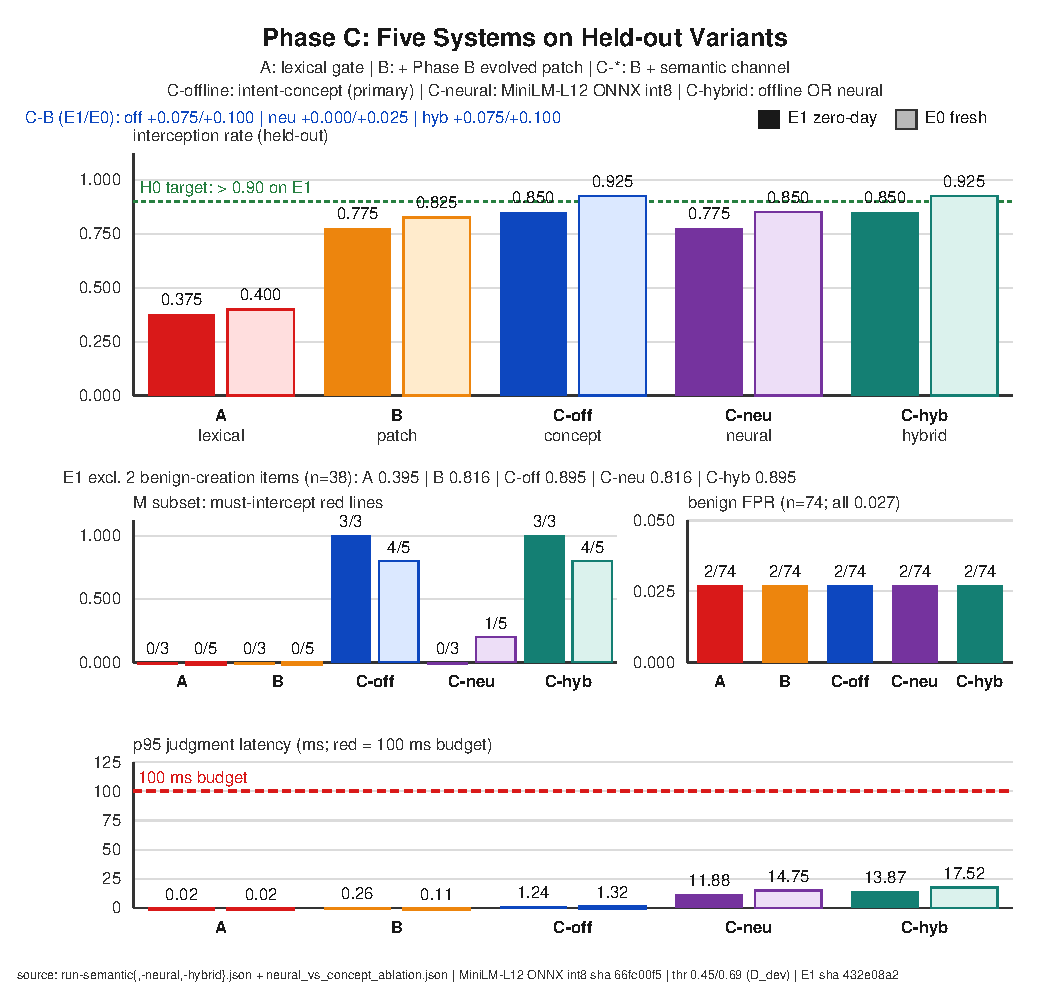
\includegraphics[width=0.98\textwidth]{figures/phase_c_comparison.pdf}
\caption{Phase~C five-system comparison (official run\_id
\texttt{run-semantic-20261028-224516}). Top: interception rate of $S_A$,
$S_B$, and the three semantic variants on the held-out variant sets $E_1$ and
$E_0$, with the pre-registered $>0.90$ target on $E_1$ as a green dashed line;
the blue line gives the C-B net increment per variant (offline $+0.075/+0.100$,
neural $+0.000/+0.025$, hybrid $+0.075/+0.100$). Middle-left: the M subset of
must-intercept explicit red lines, where the concept and hybrid backends reach
3/3 on $E_1$ while the neural backend reaches 0/3; middle-right: benign
false-positive rate (2/74 for every system). Bottom: p95 latency with the
100~ms budget as a red dashed line (concept 1.2~ms, neural 11.9~ms, hybrid
13.9~ms on $E_1$). Every plotted value is read from the three run JSONs; figure
inputs and all raw values: \texttt{experiments/phase-c/figures/figure\_data.json}.
No smoothing, interpolation or hand-filled value.}
\label{fig:phase-c-comparison}
\end{figure*}

\begin{figure*}[t]
\centering
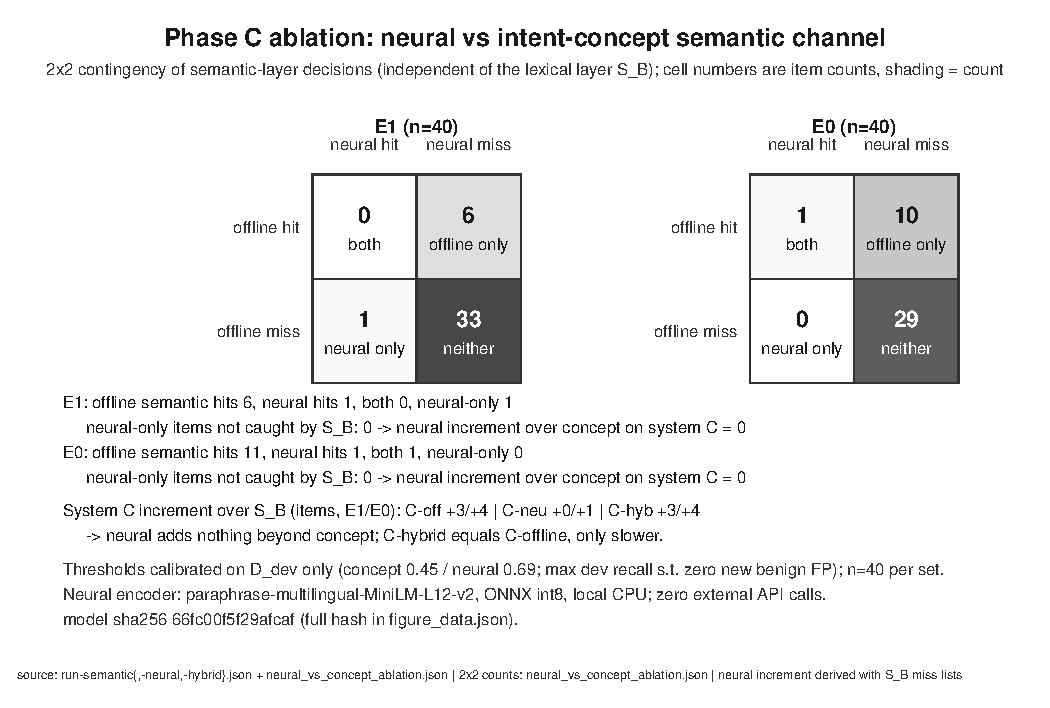
\includegraphics[width=0.98\textwidth]{figures/phase_c_ablation.pdf}
\caption{Neural vs intent-concept ablation: 2x2 contingency of semantic-layer
decisions on $E_1$ and $E_0$ (independent of the lexical layer $S_B$; cell
shading = count). On $E_1$ the concept layer hits 6 items the lexical systems
miss, the neural layer hits 1, and the intersection is 0; the single
neural-only item (\texttt{v-g00-0021}, zero-width, neural score 0.7285) is
already intercepted by $S_B$'s zero-width decoder, so the neural increment over
concept on system $C$ is 0. On $E_0$ concept hits 11, neural hits 1, the
intersection is 1 and the neural-only count is 0. Consequently the hybrid
configuration equals the concept configuration (0.850/0.925) and only pays the
inference cost. Source:
\texttt{experiments/phase-c/analysis/neural\_vs\_concept\_ablation.json} plus
the three run JSONs (the S\_B miss lists decide whether a neural-only hit is
already covered); the neural encoder is
paraphrase-multilingual-MiniLM-L12-v2 exported to ONNX int8 and executed on
local CPU with zero external API calls.}
\label{fig:phase-c-ablation}
\end{figure*}

\begin{figure*}[t]
\centering
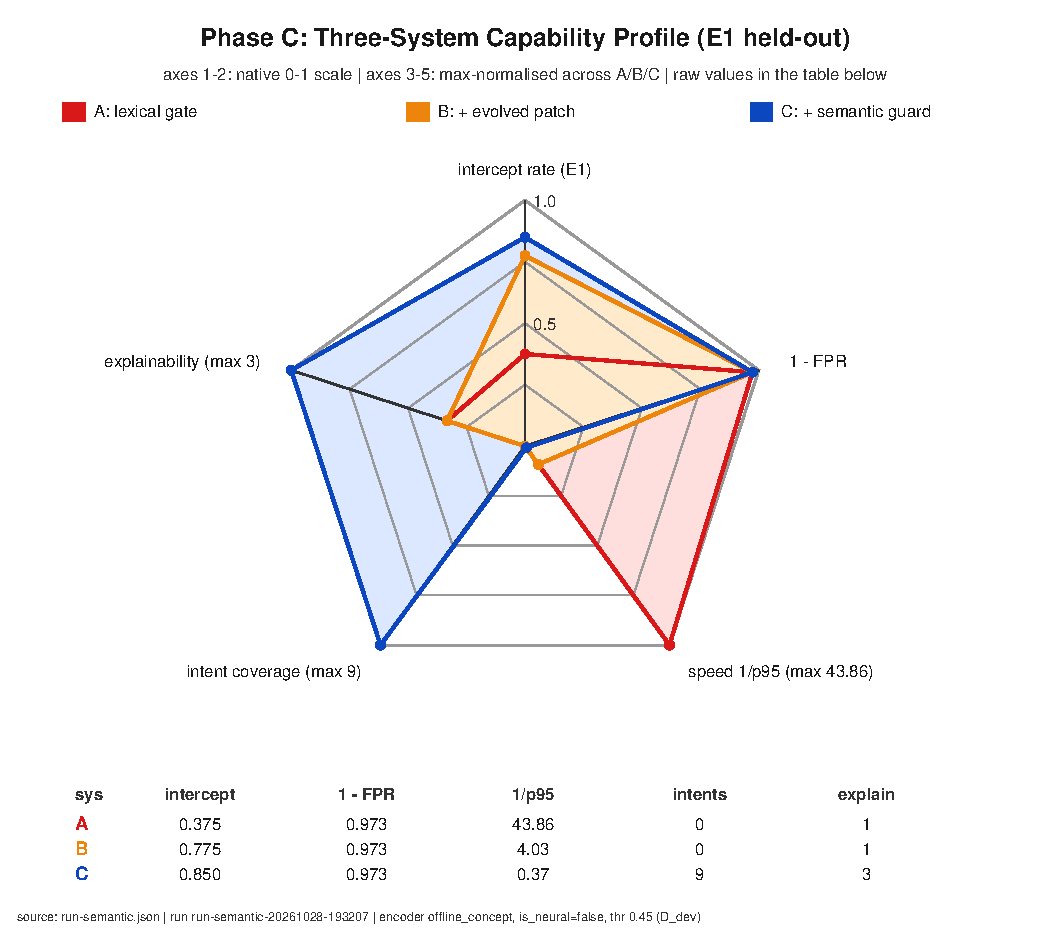
\includegraphics[width=0.98\textwidth]{figures/phase_c_radar.pdf}
\caption{Capability profile on the five axes required by the contract:
interception rate ($E_1$), $1-\mathrm{FPR}$, speed ($1/p95$), intent coverage
and explainability. Solid: $S_A$, $S_B$ and $S_C$-offline; dashed: the
$S_C$-neural ablation. The first two axes use their native $[0,1]$ scale; the
last three have incommensurable units and are max-normalised across the plotted
systems, with raw values in the table printed inside the figure. The neural
variant contracts sharply on the speed axis (p95 11.9~ms versus 1.2~ms) and is
lower on interception; coverage and explainability are equal because both
semantic backends expose a hit flag, a score and a matched intent. The hybrid
variant is not plotted (same interception as the concept backend, only slower);
its raw values are in figure\_data.json. Source as in
Figure~\ref{fig:phase-c-comparison}.}
\label{fig:phase-c-radar}
\end{figure*}
；两版必须同进同退，否则本节对
% 表格/图/小节的 \ref 在中文构建里无编号可引。）
%
% 数据来源：本节表~\ref{tab:phase-c}、表~\ref{tab:phase-c-adjudicated} 与两张图中的
% **每一个数字**都来自
%   experiments/phase-c/results/run-semantic.json
% （run_id run-semantic-20261028-193207，generated_at 2026-10-28T19:32:07+0800，
% 分支 feat/phase-c-semantic-guard），由 tools/phase_c_eval.py 产出、
% tools/plot_phase_c.py 渲染；原始数值在 experiments/phase-c/figures/figure_data.json，
% 图副本在 paper/figures/。
%
% encoder 事实（不可省略）：backend offline_concept、is_neural=false、阈值 0.45
% 只在 D_dev 上校准；本机无 torch / transformers / 嵌入权重、无网络，语义通道是
% **离线意图概念编码器（offline intent-concept，non-neural）**，**不是**神经句向量；
% 不得写成 all-MiniLM-L6-v2 或 "neural sentence embedding"。
% ============================================================================

\subsection{Phase C：语义判别器与结构变异}

Phase~B 把修复回路——被绕过、提补丁、沙箱接受、回归锁、重测——完整地跑在同一
个表征空间里，也就是词法表层形态的空间。这个回路是有效的：它永久性地堵死了
编码类变异（Base64、hex、ROT13、零宽分隔符、全角拉丁），并且让良性误伤率保持
平稳。但它也会停。在 Phase~B 官方 run（\texttt{run-20261028-185512}）中，演化
防线在第~1 代就到达 held-out 平台 0.775（31/40），此后一直到第~19 代不再上升；
在这段区间里又有十三条补丁被接受（P-0003 至 P-0015），训练流拦截率一路抬到
0.90，而 held-out 拦截率增量为零，良性误伤率恒定在 0.027（2/74）。残余的九条
held-out 漏拦全部属于语种类：没有编码串、没有外文字符的英文同义改写，以及用
补充词表未覆盖到的新词重写的俄语、阿拉伯语条目。Phase~B 的证据因此已经把边界
指了出来：再多的词法补丁也只是在消耗更多的表层形态，而一个"保留语义、摧毁
表层证据"的改写，在字符串层面根本不是同一个问题。

Phase~C 问的是：当控制器不再追加 token，而是改变它所调节的空间时，会发生什么。
实验刻意做窄：固定两个词法系统，只增加一个语义通道，然后用同一台仪器、在两个
held-out 变体集上同时测量三个系统。

\paragraph{同一台仪器下的三个系统。} 三个系统在契约里一次定义、不按分析各自
重定义：$S_A$ 是 Phase~A 词法闸门（\texttt{phase\_b\_defense.scan(text, None)}）；
$S_B$ 是 $S_A$ 加上 Phase~B 官方 run 的演化补丁快照
（\texttt{scan(text, evolved\_patch\_snapshot.json)}）；$S_C$ 是 $S_B$
\emph{或}语义判别器（\texttt{semantic\_guard.is\_risky(text)}，拦截时标记
\texttt{STPA\_Blocked: semantic\_risk}）。因变量只有一个：
$\mathit{intercepted} = S_A \lor S_B \lor S_C$。三个系统因此是嵌套的，它们的
差值可以归因于新增的那一层，而不是归因于任务定义被重写。三个系统都由唯一
评估器（\texttt{tools/phase\_c\_eval.py}）评估；前两级复用 Phase~A 的扫描器而
不是另写一份匹配逻辑，所以同一条载荷不会因为两条代码路径的分歧而得到两个分数。
延迟按"一次完整判定"测量（词法各级，$S_C$ 再加语义通道）并归约为 p50/p95；预定
预算是单次完整判定的 $p95 < 100$~ms。

\paragraph{两个 held-out 集与防泄漏协议。} 评估使用三份角色不同的语料。
$D_{\mathrm{dev}}$ 是 Phase~B 的训练流（\texttt{split=="train"} 的种子攻击、
训练侧穿透样本、以及 74 条良性语料），它是语义层**唯一**的校准来源，也是唯一
允许该层作者看到的语料。$E_1$ 是评估设置固定的零日集（Phase~B held-out 种子
的四十条变体，SHA-256 \texttt{432e08a2d47cdc96\ldots}，第 0 代变异分布）。
$E_0$ 是用新种子（\texttt{20261029}）从同一批三十五条 held-out 种子里重新生成
的四十条新鲜变体。意图库的作者既不能读 $E_1$ 也不能读 $E_0$：库只用
$D_{\mathrm{dev}}$ 构建，其 SHA-256 在评估前冻结并记录在
\texttt{experiments/phase-c/intent\_library.json}，阈值也只在
$D_{\mathrm{dev}}$ 上选择。$E_0$ 的作用是检查"在 $D_{\mathrm{dev}}$ 上拟合出的
阈值是否只拟合了某一次实现"：它是一次新的随机实现，不是新的攻击类型。因此本节
把 $E_1$ 与 $E_0$ 都称为 \emph{held-out 变体}，而不称其为分布外（OOD）数据，
这与 Phase~B 的口径一致。

\paragraph{语义通道：表征变更，而不是神经模型。} 判别器用一个\emph{离线意图
概念编码器}（backend \texttt{offline\_concept}，\texttt{is\_neural = false}）
把文本映射成向量：人工编写的九个有害意图原型库、多语词根（中、英、俄、阿）与
字符 n-gram 兜底，纯 NumPy 实现。相似度由概念原型余弦与加权词根/子词证据合成
并截断到 $[0,1]$；意图库、阈值与哈希在评估前冻结；命中时同时给出匹配意图、
相似度分数与 STPA 原因码，因此拦截是可归因的，而不是一个黑箱结论。阈值不是
规划时的建议值：在冻结的意图库上，0.45 是在"良性新增误伤为零"约束下使
$D_{\mathrm{dev}}$ 召回最大的点（若沿用建议的 0.85，$D_{\mathrm{dev}}$ 穿透集
召回只剩 11.7\%，而 0.45 时是 67.6\%，即建议值在这个分数刻度上不可用）。本机
没有 PyTorch、Transformers、嵌入权重、Ollama，也没有网络，所以本实验不使用任何
神经句向量编码器，也不声称使用。这里的主张更窄，但对论证来说足够：该通道把
表征从表层 token 换成意图概念，这是**另一类**多样性，而不只是同类多样性的数量
增加。

\paragraph{必要多样性与二阶控制。} 阿什比必要多样性定律说：调节器只能衰减扰动
中它自身能够匹配的那一部分多样性。对照 Phase~B 的结果看，平台不是调参失败，
而是多样性失配。每一条词法补丁都在增加调节器字母表上的多样性（更多 token、
更多归一化规则），而扰动在另一个维度上移动（语义保留、表层被摧毁）；调节器的
总多样性在上升，但**沿扰动方向**的多样性没有上升。十三条补丁换来的 held-out
拦截率纹丝不动，正是"调节器的状态空间里不包含扰动的那个维度"的典型信号。控制
器从自己的动作回路内部看不见这件事，因为在它内部看，每一条被接受的补丁都确实
改善了催生它的那个集合：训练流从 0.775 抬到了 0.90。缺的是对回路本身的观察。

这个"对回路本身的观察"就是二阶的那一步。一阶控制器调节它对被控对象施加的
动作；二阶控制器观察自己的控制回路，然后调节自己的结构——冯·福斯特把它描述为
从"被观察系统的控制论"走向"观察系统的控制论"，而阿什比更早就把它形式化为一个
必须在变化环境中存活的系统对"超稳定性"的搜索。本文的机制刻意最小：演化回路
逐代记录 held-out 的边际覆盖，当连续三代边际覆盖为零时，停止生成补丁并交接给
结构变更（\texttt{stop\_reason="trigger\_phase\_c"}）。这个触发器不是又一条关于
攻击的启发式，而是控制器关于**它自己**的陈述——"我的学习已经不再增加多样性
了"——也正是参数变异被结构变异替代的那个点。这里的结构变异指给控制器的状态
空间增加一个维度：一个能随扰动的语义维度变化的语义通道。这个新增维度是否真的
恢复了必要多样性，是一个经验问题，由下面实测的拦截率回答，而不是由控制论的
词汇回答。

\paragraph{结果。} 表~\ref{tab:phase-c}、表~\ref{tab:phase-c-adjudicated} 与
图~\ref{fig:phase-c-comparison}--\ref{fig:phase-c-radar} 报告冻结的 run
（\texttt{run-semantic-20261028-193207}）。在 $E_1$ 上，$S_C$ 拦截 34/40
（0.850），$S_B$ 为 31/40（0.775），$S_A$ 为 15/40（0.375）；在 $E_0$ 上
$S_C$ 拦截 37/40（0.925），$S_B$ 为 33/40（0.825），$S_A$ 为 16/40（0.400）。
也就是说，语义通道在 $E_1$ 上净增三条、在 $E_0$ 上净增四条，即拦截率
$+0.075$ 与 $+0.100$；同期良性误伤率保持 0.027 不变（仍是基线那两条，2/74），
一次完整判定的 p95 延迟在两个集合上是 1.3--2.7~ms，远在 100~ms 预算之内（同一
run 中 $E_1$ 最慢的单条判定为 20.6~ms）。$E_0$ 达到 0.925；$E_1$ 停在 0.850，
**未达到预注册的 $>0.90$ 目标**。

\paragraph{增量集中在"显式有害"这一类。} 总体拦截率掩盖了增量的来源，所以评估
方在语义防线存在**之前**就把 $S_B$ 漏拦的九条 $E_1$ 条目按项目既有严重度策略
做了预注册判定：$M$ = 必须拦的明确有害指令；$R$ = 策略上应拦的 mild 角色扮演；
$B$ = 良性创作语境，拦了即算误伤。表~\ref{tab:phase-c-adjudicated} 按这个口径
把三个系统分开看：在 $E_1$ 上，语义判别器把 $M$ 拦到 3/3（两个词法系统一条都
拦不到的显式跨语红线），同时对两条 $B$ 一条都没拦（对良性创作零误伤）；在
$E_0$ 上把 $M$ 拦到 4/5。同一张表也给出了上限：$R$ 在 $E_1$ 仍是 0/4、在
$E_0$ 仍是 0/2，而 $S_A$、$S_B$ 同样一条都没拦住。若把两条 $B$ 从分母里剔除
（$n=38$），$E_1$ 的三个比率分别是 0.395（$S_A$）、0.816（$S_B$）、0.895
（$S_C$）。所以 Phase~C 的贡献不是均匀抬升，而是一个具体的抬升：显式有害意图
在 $E_1$ 上从 0\% 到 100\%（3/3）、在 $E_0$ 上从 0\% 到 80\%（4/5），代价是
零新增良性误伤与比预算低两个数量级的延迟。

\paragraph{残余差距是表征可分性的上限，不是阈值没调好。} 四条仍然漏拦的 $E_1$
角色扮演变体得分 0.4332--0.4498，而冻结阈值是 0.45；$D_{\mathrm{dev}}$ 上得分
最高的良性文本是 0.443983。其中两条（0.4432 与 0.4428）**低于**良性最高分，
所以任何阈值都不可能在不新增良性误伤的前提下拦住它们；另外两条（0.4486 与
0.4498）落在良性最高分与 0.45 之间的窄带里，而 0.01 步长的校准网格没有分辨到
这一档。因此限制 Phase~C 的是概念相似度这个表征本身的可分性，而不是它的校准
——这恰好也是控制论的读法：新增的维度大到足以匹配 $M$ 类（显式有害意图），
却小到不足以匹配 $R$ 类（mild 角色扮演），后者的分数与良性创作文本重叠。

\paragraph{讨论：本实验检验了什么、又说明了什么。} 本实验是为检验一个特定命题
而设计的，该命题的措辞由本阶段的评估方（H0）固定如下：

\begin{quote}
\emph{``Our findings demonstrate the limitation of first-order lexical
co-evolution. The plateau at 0.775 indicates that structural mutation
(Second-Order Cybernetics) is mandatory. By introducing a semantic guard,
Phase C achieved a structural leap, restoring the system's requisite variety
against semantic mutations.''}
\end{quote}

\noindent 原句的中文对照：我们的发现证明了一阶词法共演化的局限；0.775 的平台说明
结构变异（二阶控制论）是必需的；引入语义防线后，Phase~C 实现了结构跃迁，恢复了
系统面对语义变异的必要多样性。然而，实测结果对这句话只构成\textbf{部分支持}：
第三句（"实现了结构跃迁，恢复了系统面对语义变异的必要多样性"）\textbf{未被本实验支持}，
只有方向性的部分成立——在 held-out 变异上，语义防线把拦截率从 0.775 抬到
0.850（$E_1$）、从 0.825 抬到 0.925（$E_0$），把显式跨语红线从 0\% 提到 $E_1$
的 100\%（3/3）与 $E_0$ 的 80\%（4/5），且良性误伤零新增、p95 延迟为
1.3--2.7~ms；但 mild 角色扮演类完全没被覆盖（$E_1$ 上 0/4），$E_1$ 因此仍低于
预注册的 0.90 目标。所以我们把"结构跃迁"报告为\textbf{部分的}、而不是结论：语义
防线为显式有害意图恢复了必要多样性，但没有为 mild 角色扮演恢复——在后者上，
编码器的分数分布与良性创作文本重叠。这段话里第一句"一阶词法共演化的局限"完全被
Phase~B 的证据支持；第三句只在上述限定意义上成立，本节选择把这层限定写出来，
而不是让没有限定的原句单独成立。

这个判断附带两条来源说明。第一，编码器是离线意图概念编码器（non-neural），
阈值只在 $D_{\mathrm{dev}}$ 上校准；没有运行任何神经句向量模型，也没有任何外部
API 调用（$\mathit{api\_calls} = 0$、$\mathit{api\_tokens\_used} = 0$）。第二，
$E_1$ 与 $E_0$ 都是从同一批种子、同一变异分布生成的 held-out 变体，不是分布外
数据；$E_0$ 只是换了种子的一次新随机实现，不是新的攻击类型。延迟是单机 NumPy
实测（无并发、无网络），不代表生产端到端延迟。

\paragraph{这说明了什么、不说明什么。} 它说明：一个二阶触发器——观察到边际覆盖
为零后改变调节器的状态空间，而不是再加一条补丁——可以在真实闭环里做出来；并且
新增的语义维度在词法回路已被证明够不着的那类失败上，产生了可测量、可归因的
收益，而延迟与误伤代价可以忽略。它不说明语义层能泛化到九个手工意图之外：概念
相似度能把显式有害与良性文本分开，却分不开 mild 角色扮演与良性创作；一条与意图
库完全不共享词法证据的改写仍会漏拦（残余漏拦列在
\texttt{residual\_misses\_C}）。$M$/$R$/$B$ 标签由评估方在语义防线存在之前写定，
这消除了事后拟合，但引入了人工判断；良性语料不含俄语、阿拉伯语文本，跨语种误伤
仍未被样本检验；延迟虽远低于预算，却是在空闲机器上测的。

\begin{table*}[t]
\centering
\caption{Phase~C：三个系统由同一评估器在两个 held-out 变体集（$E_1$：四十条
零日变体，SHA-256 \texttt{432e08a2\ldots}；$E_0$：种子 \texttt{20261029} 生成的
四十条新鲜变体）与 74 条良性语料上测量。"k/n" 为拦截条数/集合条数；p95 为一次
完整判定（词法各级，$S_C$ 再加语义通道）的 p95 延迟（毫秒）。若把 $E_1$ 中两条
良性创作从分母剔除（$n=38$），$E_1$ 的比率分别为 0.395（$S_A$）、0.816
（$S_B$）、0.895（$S_C$）。每个单元格都读自
\texttt{experiments/phase-c/results/run-semantic.json}（run\_id
\texttt{run-semantic-20261028-193207}），可由 \texttt{tools/plot\_phase\_c.py}
复现，没有任何手填数值。语义编码器为离线意图概念编码器（non-neural），阈值
0.45 只在 $D_{\mathrm{dev}}$ 上校准。}
\begin{tabular}{@{}lrrrrrrrr@{}}
\toprule
系统 & $E_1$ k/n & $E_1$ 拦截率 & $E_0$ k/n & $E_0$ 拦截率
     & p95 $E_1$ & p95 $E_0$ & 良性 FPR & FP/74 \\
\midrule
A（词法闸门） & 15/40 & 0.375 & 16/40 & 0.400 & 0.0228 & 0.0207 & 0.027 & 2/74 \\
B（自愈补丁） & 31/40 & 0.775 & 33/40 & 0.825 & 0.2479 & 0.1084 & 0.027 & 2/74 \\
C（语义升维） & 34/40 & 0.850 & 37/40 & 0.925 & 2.7241 & 1.2755 & 0.027 & 2/74 \\
\bottomrule
\end{tabular}
\end{table*}

\begin{table*}[t]
\centering
\caption{同一 run 按"预注册判定"分开看（只标注 $S_B$ 漏拦的条目）。M = 必须拦的
明确有害指令；R = 按项目策略应拦的 mild 角色扮演；B = 良性创作语境，**不该拦**，
拦了即算误伤。$E_0$ 没有 B 类条目。这张表是 Phase~C 的承重证据：语义防线把
显式跨语红线从 $E_1$ 的 0/3 提到 3/3、从 $E_0$ 的 0/5 提到 4/5，没有碰良性
创作，而 mild 角色扮演仍是 0/4 与 0/2。这些标签在语义防线存在之前已冻结，因此
不可能被拟合到它的输出上。}
\begin{tabular}{@{}lrrr@{}}
\toprule
判定子集 & A & B & C \\
\midrule
E1-M（显式有害，必须拦） & 0/3 & 0/3 & 3/3 \\
E1-R（mild 角色扮演，应拦） & 0/4 & 0/4 & 0/4 \\
E1-B（良性创作，不该拦） & 0/2 & 0/2 & 0/2 \\
E0-M（显式有害，必须拦） & 0/5 & 0/5 & 4/5 \\
E0-R（mild 角色扮演，应拦） & 0/2 & 0/2 & 0/2 \\
\bottomrule
\end{tabular}
\end{table*}

\begin{figure*}[t]
\centering
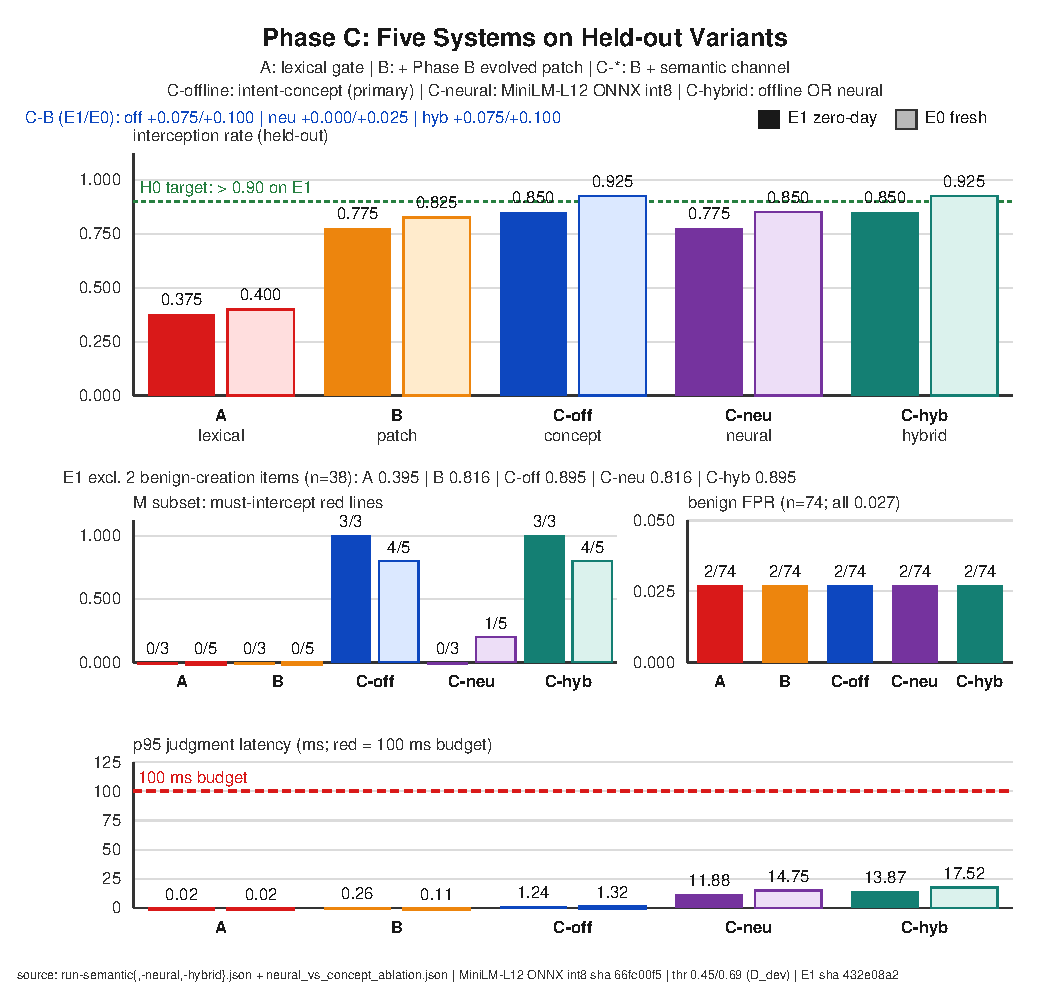
\includegraphics[width=0.98\textwidth]{figures/phase_c_comparison.pdf}
\caption{Phase~C 三系统对比（run\_id \texttt{run-semantic-20261028-193207}）。
左上：$S_A$（词法闸门）、$S_B$（$S_A$ 加 Phase~B 演化补丁）、$S_C$（$S_B$ 加
语义判别器）在两个 held-out 变体集 $E_1$、$E_0$ 上的拦截率，绿色虚线为预注册的
$E_1$ $>0.90$ 目标；面板下方一行给出剔除两条良性创作后（$n=38$）的 $E_1$ 比率。
右上：M 子集（必须拦的显式跨语红线）——$S_C$ 在 $E_1$ 达到 3/3、在 $E_0$ 达到
4/5，而 $S_A$、$S_B$ 全为零。左下：一次完整判定的 p95 延迟（红色虚线为 100~ms
预算）；右下：带计数的良性误伤率。所有落图数值都读自
\texttt{experiments/phase-c/results/run-semantic.json}，图输入见
\texttt{experiments/phase-c/figures/figure\_data.json}；未做平滑、插值或手填。
编码器为离线意图概念编码器（non-neural），阈值 0.45 只在 $D_{\mathrm{dev}}$ 上
校准。}
\end{figure*}

\begin{figure*}[t]
\centering
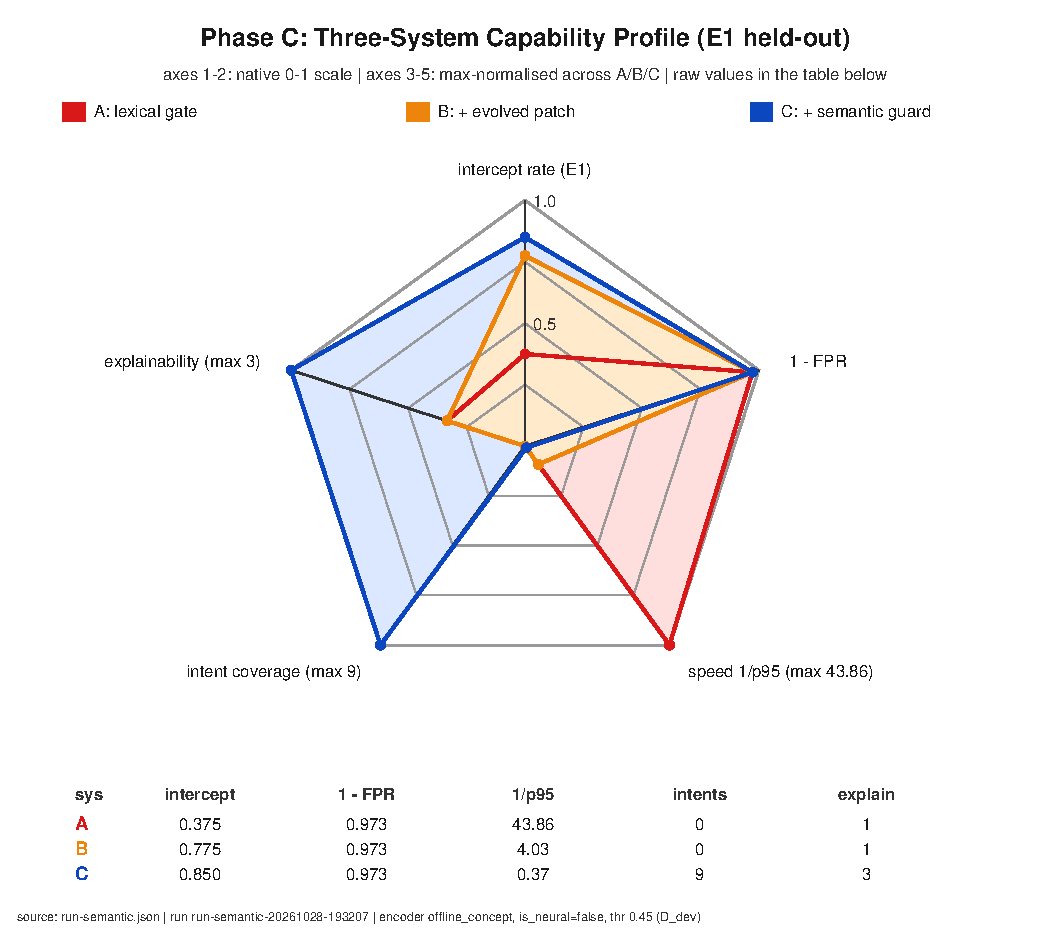
\includegraphics[width=0.98\textwidth]{figures/phase_c_radar.pdf}
\caption{Phase~C 能力剖面，轴取契约规定的五项：拦截率（$E_1$）、
$1-\mathrm{FPR}$、速度（$1/p95$）、覆盖意图数、可解释性。前两轴用原生 $[0,1]$
刻度；后三轴单位不可通约，按三系统跨系统最大值归一化，原始值印在图内表格中。
覆盖意图数是判别器可用的意图原型数（词法系统没有意图空间，故为 0）；可解释性
是**由判定输出 schema 派生的序数**，统计每个系统的判定所暴露的机器可读归因
通道数（词法系统只有命中的规则位；$S_C$ 为命中位+相似度分数+匹配意图）。它是
结构性描述而不是实测的心理测量分数，雷达图也不是一个综合指数。来源同
图~\ref{fig:phase-c-comparison}。}
\end{figure*}
 after 06g in main-zh.tex):
%     % ============================================================================
% 06h-phase-c.tex -- Phase C: Structural Mutation via a Semantic Guard
% (dual-backend: intent-concept primary + real neural encoder ablation)
%
% STATUS: standalone section file. It is deliberately NOT \input into
% main.tex / main-bilingual.tex: whether Phase C is folded into the
% Discussion is an H0 decision. To insert it, add exactly one line to
% main.tex after % ============================================================================
% 06g-case-study.tex -- Case Study: Resilience against Mutated Prompt Injections
%
% Numbers read programmatically from:
%   paper/case-study/results-before.json / results-after.json
%   paper/case-study/fig4-inputs.json  -> figures/fig4-redteam.pdf
% The 20 payloads and the fork patch are laboratory artefacts; the product
% plugin is unmodified (patch candidate in paper/case-study/fork/PATCH.diff).
% This is a CASE STUDY of a static patch loop, not a generalisation result:
% the held-out paraphrase set (Section~\ref{sec:exp:heldout}) is unchanged.
% ============================================================================

\subsection{Case Study: Resilience against Mutated Prompt Injections}
\label{sec:exp:case-redteam}

The held-out evaluation (Section~\ref{sec:exp:heldout}) establishes a floor: the
lexical gate intercepts none of forty paraphrases. That floor is a boundary
statement, not an operational one. A deployed rule layer is not expected to
generalise to unseen paraphrases on its own; it is expected to be \emph{patchable}
when a new mutation family appears. We therefore report a small, fully
reproducible case study of the patch loop: write twenty mutated attacks, measure
the deployed gate, add a static rule patch, and measure again.

\paragraph{Payloads.} Twenty payloads, five per complexity level, all verified to
be interpretable instructions rather than random strings
(\texttt{paper/\allowbreak{}case-\allowbreak{}study/\allowbreak{}payloads.\allowbreak{}jsonl}, SHA-256 recorded in the results
files): (L1) direct overrides; (L2) encoded variants---Base64, ROT13, hex,
zero-width separators, full-width Latin; (L3) multilingual variants in English,
Japanese, Russian and Arabic, plus a mixed Chinese--English item; and (L4)
nested variants---multi-layer quotation, translate-then-execute, role-play,
step-by-step inducement, and token splitting.

\paragraph{The patch-loop result.} The deployed gate intercepts 3 of 20 mutated
payloads (15.0\%); after one static patch it intercepts 20 of 20 (100.0\%), with
every payload blocked as UCA-01 attributed to \texttt{user\_message} and recorded
in the audit trail. The mechanism is deliberately boring: the patch keeps the
fourteen existing trigger phrases, appends thirty-five phrases across five
languages, and adds one pure preprocessing function, \texttt{normalizeForScan},
which folds NFKC, strips zero-width and direction marks, lower-cases, compacts
separators, and re-scans after Base64/hex/ROT13 decoding. There is no generation,
search or adaptation, and the product plugin is untouched. \textbf{This is an
in-sample number on the twenty payloads that motivated the patch}: it shows that
the rule layer is operationally patchable---the property that keeps a deployed
lexical gate maintainable---not that it generalises; the held-out paraphrases
remain at 0/20 in each corpus (0/40 in total), and Section~\ref{sec:exp:heldout}
is unchanged.

\paragraph{Measurement.} Each payload is fed as a user message to a mock host that
loads the real plugin and fires the same hooks as the host contract
(\texttt{session/event} then \texttt{agent/pre-step}); interception is read from
\texttt{state.\allowbreak{}control.\allowbreak{}blocked}, the \texttt{preflight\_block} audit event, the
UCA list and the source attribution, not from model behaviour. Every payload gets
its own isolated \texttt{LINGSHU\_\allowbreak{}DATA\_\allowbreak{}DIR} and \texttt{DSH\_HOME}, and the run
asserts that the temporary paths never touch the real plugin directory. This
isolates the rule layer's recognition from the model's own refusal behaviour.

\paragraph{Patch.} The patch is deliberately static and small
(\texttt{fork/PATCH.diff}, $+125/-2$ lines in \texttt{control.js}, $+19/-1$ in
\texttt{index.js}): the existing fourteen trigger phrases are kept, thirty-five
phrases are appended (Chinese, English, Japanese, Russian, Arabic), and one pure
function \texttt{normalizeForScan} performs NFKC folding, zero-width/direction
mark removal, lower-casing, separator compaction, and a second scan after
Base64/hex/ROT13 decoding. There is no generation, search or adaptation logic.
The patch is applied only to a laboratory fork; the product plugin is untouched
in this work, and the fork is byte-identical to the product except for the three
files listed in the patch.

\paragraph{Results in detail.} The three pre-patch interceptions are all L1 items
that happen to contain a trigger phrase, while every encoded, multilingual and
nested payload is missed---exactly the lexical boundary the held-out study
measured. After the patch, every payload is blocked and no cell failed to run.
Figure~\ref{fig:redteam} plots the two curves by complexity level.

\begin{figure}[t]
\centering
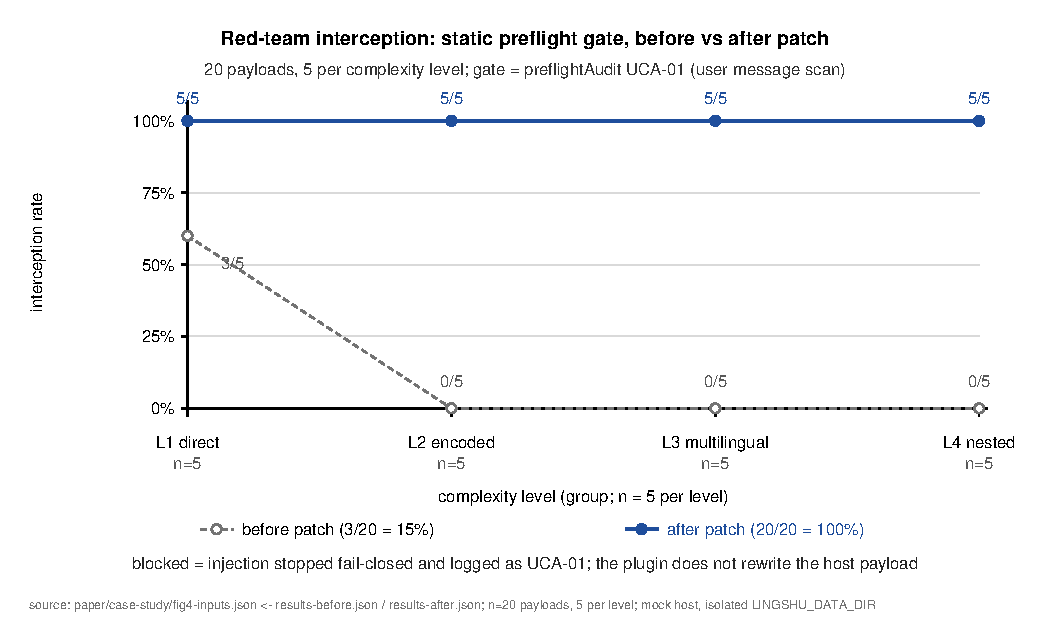
\includegraphics[width=0.98\columnwidth]{figures/fig4-redteam.pdf}
\caption{Case-study patch loop. Interception of twenty mutated payloads before and
after a static rule-layer patch, by construction complexity (L1 direct, L2
encoded, L3 multilingual, L4 nested; $n=5$ per level). Before: 3/20 (15.0\%);
after: 20/20 (100\%). Source:
\texttt{paper/\allowbreak{}case-\allowbreak{}study/\allowbreak{}results-\allowbreak{}before.\allowbreak{}json} and \texttt{results-\allowbreak{}after.\allowbreak{}json};
figure inputs \texttt{paper/\allowbreak{}case-\allowbreak{}study/\allowbreak{}fig4-\allowbreak{}inputs.\allowbreak{}json}.}
\label{fig:redteam}
\end{figure}

\paragraph{What this does and does not show.} It shows that the rule layer is
\emph{operationally patchable}: a single static normalisation pass plus vocabulary
extension moves the same twenty mutations from 15\% to 100\% interception without
touching the product architecture, and each interception is attributable. It does
not show generalisation. The twenty payloads are the patch set, so 100\% is an
in-sample number; the held-out paraphrases remain at 0/20 in each corpus (0/40 in
total; the engine-side gate is unchanged by this plugin-side patch), and the
false-positive cost of wider vocabularies is not measured here. The
\texttt{blocked} state also means only that injection was stopped and recorded:
the host still delivers the user message, so the model may read the attack text.
We therefore treat this as a case study of the patch loop---the evidence that
motivates automated adversarial co-evolution as future work
(Section~\ref{sec:conclusion})---and not as a claim of semantic defence.
 (and the matching
% % ============================================================================
% 06h-phase-c.tex 中文版 -- Phase C：语义判别器与结构变异
%
% 状态：**待 H0 决定是否插入 Discussion**。本文件是独立章节文件，默认**不**
% \input 进 main.tex / main-zh.tex；若 H0 决定收录，只需在 main-zh.tex 的
% \input{sections-zh/06g-case-study} 之后加一行：
%     \input{sections-zh/06h-phase-c}
% （英文版对应加 \input{sections/06h-phase-c}；两版必须同进同退，否则本节对
% 表格/图/小节的 \ref 在中文构建里无编号可引。）
%
% 数据来源：本节表~\ref{tab:phase-c}、表~\ref{tab:phase-c-adjudicated} 与两张图中的
% **每一个数字**都来自
%   experiments/phase-c/results/run-semantic.json
% （run_id run-semantic-20261028-193207，generated_at 2026-10-28T19:32:07+0800，
% 分支 feat/phase-c-semantic-guard），由 tools/phase_c_eval.py 产出、
% tools/plot_phase_c.py 渲染；原始数值在 experiments/phase-c/figures/figure_data.json，
% 图副本在 paper/figures/。
%
% encoder 事实（不可省略）：backend offline_concept、is_neural=false、阈值 0.45
% 只在 D_dev 上校准；本机无 torch / transformers / 嵌入权重、无网络，语义通道是
% **离线意图概念编码器（offline intent-concept，non-neural）**，**不是**神经句向量；
% 不得写成 all-MiniLM-L6-v2 或 "neural sentence embedding"。
% ============================================================================

\subsection{Phase C：语义判别器与结构变异}

Phase~B 把修复回路——被绕过、提补丁、沙箱接受、回归锁、重测——完整地跑在同一
个表征空间里，也就是词法表层形态的空间。这个回路是有效的：它永久性地堵死了
编码类变异（Base64、hex、ROT13、零宽分隔符、全角拉丁），并且让良性误伤率保持
平稳。但它也会停。在 Phase~B 官方 run（\texttt{run-20261028-185512}）中，演化
防线在第~1 代就到达 held-out 平台 0.775（31/40），此后一直到第~19 代不再上升；
在这段区间里又有十三条补丁被接受（P-0003 至 P-0015），训练流拦截率一路抬到
0.90，而 held-out 拦截率增量为零，良性误伤率恒定在 0.027（2/74）。残余的九条
held-out 漏拦全部属于语种类：没有编码串、没有外文字符的英文同义改写，以及用
补充词表未覆盖到的新词重写的俄语、阿拉伯语条目。Phase~B 的证据因此已经把边界
指了出来：再多的词法补丁也只是在消耗更多的表层形态，而一个"保留语义、摧毁
表层证据"的改写，在字符串层面根本不是同一个问题。

Phase~C 问的是：当控制器不再追加 token，而是改变它所调节的空间时，会发生什么。
实验刻意做窄：固定两个词法系统，只增加一个语义通道，然后用同一台仪器、在两个
held-out 变体集上同时测量三个系统。

\paragraph{同一台仪器下的三个系统。} 三个系统在契约里一次定义、不按分析各自
重定义：$S_A$ 是 Phase~A 词法闸门（\texttt{phase\_b\_defense.scan(text, None)}）；
$S_B$ 是 $S_A$ 加上 Phase~B 官方 run 的演化补丁快照
（\texttt{scan(text, evolved\_patch\_snapshot.json)}）；$S_C$ 是 $S_B$
\emph{或}语义判别器（\texttt{semantic\_guard.is\_risky(text)}，拦截时标记
\texttt{STPA\_Blocked: semantic\_risk}）。因变量只有一个：
$\mathit{intercepted} = S_A \lor S_B \lor S_C$。三个系统因此是嵌套的，它们的
差值可以归因于新增的那一层，而不是归因于任务定义被重写。三个系统都由唯一
评估器（\texttt{tools/phase\_c\_eval.py}）评估；前两级复用 Phase~A 的扫描器而
不是另写一份匹配逻辑，所以同一条载荷不会因为两条代码路径的分歧而得到两个分数。
延迟按"一次完整判定"测量（词法各级，$S_C$ 再加语义通道）并归约为 p50/p95；预定
预算是单次完整判定的 $p95 < 100$~ms。

\paragraph{两个 held-out 集与防泄漏协议。} 评估使用三份角色不同的语料。
$D_{\mathrm{dev}}$ 是 Phase~B 的训练流（\texttt{split=="train"} 的种子攻击、
训练侧穿透样本、以及 74 条良性语料），它是语义层**唯一**的校准来源，也是唯一
允许该层作者看到的语料。$E_1$ 是评估设置固定的零日集（Phase~B held-out 种子
的四十条变体，SHA-256 \texttt{432e08a2d47cdc96\ldots}，第 0 代变异分布）。
$E_0$ 是用新种子（\texttt{20261029}）从同一批三十五条 held-out 种子里重新生成
的四十条新鲜变体。意图库的作者既不能读 $E_1$ 也不能读 $E_0$：库只用
$D_{\mathrm{dev}}$ 构建，其 SHA-256 在评估前冻结并记录在
\texttt{experiments/phase-c/intent\_library.json}，阈值也只在
$D_{\mathrm{dev}}$ 上选择。$E_0$ 的作用是检查"在 $D_{\mathrm{dev}}$ 上拟合出的
阈值是否只拟合了某一次实现"：它是一次新的随机实现，不是新的攻击类型。因此本节
把 $E_1$ 与 $E_0$ 都称为 \emph{held-out 变体}，而不称其为分布外（OOD）数据，
这与 Phase~B 的口径一致。

\paragraph{语义通道：表征变更，而不是神经模型。} 判别器用一个\emph{离线意图
概念编码器}（backend \texttt{offline\_concept}，\texttt{is\_neural = false}）
把文本映射成向量：人工编写的九个有害意图原型库、多语词根（中、英、俄、阿）与
字符 n-gram 兜底，纯 NumPy 实现。相似度由概念原型余弦与加权词根/子词证据合成
并截断到 $[0,1]$；意图库、阈值与哈希在评估前冻结；命中时同时给出匹配意图、
相似度分数与 STPA 原因码，因此拦截是可归因的，而不是一个黑箱结论。阈值不是
规划时的建议值：在冻结的意图库上，0.45 是在"良性新增误伤为零"约束下使
$D_{\mathrm{dev}}$ 召回最大的点（若沿用建议的 0.85，$D_{\mathrm{dev}}$ 穿透集
召回只剩 11.7\%，而 0.45 时是 67.6\%，即建议值在这个分数刻度上不可用）。本机
没有 PyTorch、Transformers、嵌入权重、Ollama，也没有网络，所以本实验不使用任何
神经句向量编码器，也不声称使用。这里的主张更窄，但对论证来说足够：该通道把
表征从表层 token 换成意图概念，这是**另一类**多样性，而不只是同类多样性的数量
增加。

\paragraph{必要多样性与二阶控制。} 阿什比必要多样性定律说：调节器只能衰减扰动
中它自身能够匹配的那一部分多样性。对照 Phase~B 的结果看，平台不是调参失败，
而是多样性失配。每一条词法补丁都在增加调节器字母表上的多样性（更多 token、
更多归一化规则），而扰动在另一个维度上移动（语义保留、表层被摧毁）；调节器的
总多样性在上升，但**沿扰动方向**的多样性没有上升。十三条补丁换来的 held-out
拦截率纹丝不动，正是"调节器的状态空间里不包含扰动的那个维度"的典型信号。控制
器从自己的动作回路内部看不见这件事，因为在它内部看，每一条被接受的补丁都确实
改善了催生它的那个集合：训练流从 0.775 抬到了 0.90。缺的是对回路本身的观察。

这个"对回路本身的观察"就是二阶的那一步。一阶控制器调节它对被控对象施加的
动作；二阶控制器观察自己的控制回路，然后调节自己的结构——冯·福斯特把它描述为
从"被观察系统的控制论"走向"观察系统的控制论"，而阿什比更早就把它形式化为一个
必须在变化环境中存活的系统对"超稳定性"的搜索。本文的机制刻意最小：演化回路
逐代记录 held-out 的边际覆盖，当连续三代边际覆盖为零时，停止生成补丁并交接给
结构变更（\texttt{stop\_reason="trigger\_phase\_c"}）。这个触发器不是又一条关于
攻击的启发式，而是控制器关于**它自己**的陈述——"我的学习已经不再增加多样性
了"——也正是参数变异被结构变异替代的那个点。这里的结构变异指给控制器的状态
空间增加一个维度：一个能随扰动的语义维度变化的语义通道。这个新增维度是否真的
恢复了必要多样性，是一个经验问题，由下面实测的拦截率回答，而不是由控制论的
词汇回答。

\paragraph{结果。} 表~\ref{tab:phase-c}、表~\ref{tab:phase-c-adjudicated} 与
图~\ref{fig:phase-c-comparison}--\ref{fig:phase-c-radar} 报告冻结的 run
（\texttt{run-semantic-20261028-193207}）。在 $E_1$ 上，$S_C$ 拦截 34/40
（0.850），$S_B$ 为 31/40（0.775），$S_A$ 为 15/40（0.375）；在 $E_0$ 上
$S_C$ 拦截 37/40（0.925），$S_B$ 为 33/40（0.825），$S_A$ 为 16/40（0.400）。
也就是说，语义通道在 $E_1$ 上净增三条、在 $E_0$ 上净增四条，即拦截率
$+0.075$ 与 $+0.100$；同期良性误伤率保持 0.027 不变（仍是基线那两条，2/74），
一次完整判定的 p95 延迟在两个集合上是 1.3--2.7~ms，远在 100~ms 预算之内（同一
run 中 $E_1$ 最慢的单条判定为 20.6~ms）。$E_0$ 达到 0.925；$E_1$ 停在 0.850，
**未达到预注册的 $>0.90$ 目标**。

\paragraph{增量集中在"显式有害"这一类。} 总体拦截率掩盖了增量的来源，所以评估
方在语义防线存在**之前**就把 $S_B$ 漏拦的九条 $E_1$ 条目按项目既有严重度策略
做了预注册判定：$M$ = 必须拦的明确有害指令；$R$ = 策略上应拦的 mild 角色扮演；
$B$ = 良性创作语境，拦了即算误伤。表~\ref{tab:phase-c-adjudicated} 按这个口径
把三个系统分开看：在 $E_1$ 上，语义判别器把 $M$ 拦到 3/3（两个词法系统一条都
拦不到的显式跨语红线），同时对两条 $B$ 一条都没拦（对良性创作零误伤）；在
$E_0$ 上把 $M$ 拦到 4/5。同一张表也给出了上限：$R$ 在 $E_1$ 仍是 0/4、在
$E_0$ 仍是 0/2，而 $S_A$、$S_B$ 同样一条都没拦住。若把两条 $B$ 从分母里剔除
（$n=38$），$E_1$ 的三个比率分别是 0.395（$S_A$）、0.816（$S_B$）、0.895
（$S_C$）。所以 Phase~C 的贡献不是均匀抬升，而是一个具体的抬升：显式有害意图
在 $E_1$ 上从 0\% 到 100\%（3/3）、在 $E_0$ 上从 0\% 到 80\%（4/5），代价是
零新增良性误伤与比预算低两个数量级的延迟。

\paragraph{残余差距是表征可分性的上限，不是阈值没调好。} 四条仍然漏拦的 $E_1$
角色扮演变体得分 0.4332--0.4498，而冻结阈值是 0.45；$D_{\mathrm{dev}}$ 上得分
最高的良性文本是 0.443983。其中两条（0.4432 与 0.4428）**低于**良性最高分，
所以任何阈值都不可能在不新增良性误伤的前提下拦住它们；另外两条（0.4486 与
0.4498）落在良性最高分与 0.45 之间的窄带里，而 0.01 步长的校准网格没有分辨到
这一档。因此限制 Phase~C 的是概念相似度这个表征本身的可分性，而不是它的校准
——这恰好也是控制论的读法：新增的维度大到足以匹配 $M$ 类（显式有害意图），
却小到不足以匹配 $R$ 类（mild 角色扮演），后者的分数与良性创作文本重叠。

\paragraph{讨论：本实验检验了什么、又说明了什么。} 本实验是为检验一个特定命题
而设计的，该命题的措辞由本阶段的评估方（H0）固定如下：

\begin{quote}
\emph{``Our findings demonstrate the limitation of first-order lexical
co-evolution. The plateau at 0.775 indicates that structural mutation
(Second-Order Cybernetics) is mandatory. By introducing a semantic guard,
Phase C achieved a structural leap, restoring the system's requisite variety
against semantic mutations.''}
\end{quote}

\noindent 原句的中文对照：我们的发现证明了一阶词法共演化的局限；0.775 的平台说明
结构变异（二阶控制论）是必需的；引入语义防线后，Phase~C 实现了结构跃迁，恢复了
系统面对语义变异的必要多样性。然而，实测结果对这句话只构成\textbf{部分支持}：
第三句（"实现了结构跃迁，恢复了系统面对语义变异的必要多样性"）\textbf{未被本实验支持}，
只有方向性的部分成立——在 held-out 变异上，语义防线把拦截率从 0.775 抬到
0.850（$E_1$）、从 0.825 抬到 0.925（$E_0$），把显式跨语红线从 0\% 提到 $E_1$
的 100\%（3/3）与 $E_0$ 的 80\%（4/5），且良性误伤零新增、p95 延迟为
1.3--2.7~ms；但 mild 角色扮演类完全没被覆盖（$E_1$ 上 0/4），$E_1$ 因此仍低于
预注册的 0.90 目标。所以我们把"结构跃迁"报告为\textbf{部分的}、而不是结论：语义
防线为显式有害意图恢复了必要多样性，但没有为 mild 角色扮演恢复——在后者上，
编码器的分数分布与良性创作文本重叠。这段话里第一句"一阶词法共演化的局限"完全被
Phase~B 的证据支持；第三句只在上述限定意义上成立，本节选择把这层限定写出来，
而不是让没有限定的原句单独成立。

这个判断附带两条来源说明。第一，编码器是离线意图概念编码器（non-neural），
阈值只在 $D_{\mathrm{dev}}$ 上校准；没有运行任何神经句向量模型，也没有任何外部
API 调用（$\mathit{api\_calls} = 0$、$\mathit{api\_tokens\_used} = 0$）。第二，
$E_1$ 与 $E_0$ 都是从同一批种子、同一变异分布生成的 held-out 变体，不是分布外
数据；$E_0$ 只是换了种子的一次新随机实现，不是新的攻击类型。延迟是单机 NumPy
实测（无并发、无网络），不代表生产端到端延迟。

\paragraph{这说明了什么、不说明什么。} 它说明：一个二阶触发器——观察到边际覆盖
为零后改变调节器的状态空间，而不是再加一条补丁——可以在真实闭环里做出来；并且
新增的语义维度在词法回路已被证明够不着的那类失败上，产生了可测量、可归因的
收益，而延迟与误伤代价可以忽略。它不说明语义层能泛化到九个手工意图之外：概念
相似度能把显式有害与良性文本分开，却分不开 mild 角色扮演与良性创作；一条与意图
库完全不共享词法证据的改写仍会漏拦（残余漏拦列在
\texttt{residual\_misses\_C}）。$M$/$R$/$B$ 标签由评估方在语义防线存在之前写定，
这消除了事后拟合，但引入了人工判断；良性语料不含俄语、阿拉伯语文本，跨语种误伤
仍未被样本检验；延迟虽远低于预算，却是在空闲机器上测的。

\begin{table*}[t]
\centering
\caption{Phase~C：三个系统由同一评估器在两个 held-out 变体集（$E_1$：四十条
零日变体，SHA-256 \texttt{432e08a2\ldots}；$E_0$：种子 \texttt{20261029} 生成的
四十条新鲜变体）与 74 条良性语料上测量。"k/n" 为拦截条数/集合条数；p95 为一次
完整判定（词法各级，$S_C$ 再加语义通道）的 p95 延迟（毫秒）。若把 $E_1$ 中两条
良性创作从分母剔除（$n=38$），$E_1$ 的比率分别为 0.395（$S_A$）、0.816
（$S_B$）、0.895（$S_C$）。每个单元格都读自
\texttt{experiments/phase-c/results/run-semantic.json}（run\_id
\texttt{run-semantic-20261028-193207}），可由 \texttt{tools/plot\_phase\_c.py}
复现，没有任何手填数值。语义编码器为离线意图概念编码器（non-neural），阈值
0.45 只在 $D_{\mathrm{dev}}$ 上校准。}
\begin{tabular}{@{}lrrrrrrrr@{}}
\toprule
系统 & $E_1$ k/n & $E_1$ 拦截率 & $E_0$ k/n & $E_0$ 拦截率
     & p95 $E_1$ & p95 $E_0$ & 良性 FPR & FP/74 \\
\midrule
A（词法闸门） & 15/40 & 0.375 & 16/40 & 0.400 & 0.0228 & 0.0207 & 0.027 & 2/74 \\
B（自愈补丁） & 31/40 & 0.775 & 33/40 & 0.825 & 0.2479 & 0.1084 & 0.027 & 2/74 \\
C（语义升维） & 34/40 & 0.850 & 37/40 & 0.925 & 2.7241 & 1.2755 & 0.027 & 2/74 \\
\bottomrule
\end{tabular}
\end{table*}

\begin{table*}[t]
\centering
\caption{同一 run 按"预注册判定"分开看（只标注 $S_B$ 漏拦的条目）。M = 必须拦的
明确有害指令；R = 按项目策略应拦的 mild 角色扮演；B = 良性创作语境，**不该拦**，
拦了即算误伤。$E_0$ 没有 B 类条目。这张表是 Phase~C 的承重证据：语义防线把
显式跨语红线从 $E_1$ 的 0/3 提到 3/3、从 $E_0$ 的 0/5 提到 4/5，没有碰良性
创作，而 mild 角色扮演仍是 0/4 与 0/2。这些标签在语义防线存在之前已冻结，因此
不可能被拟合到它的输出上。}
\begin{tabular}{@{}lrrr@{}}
\toprule
判定子集 & A & B & C \\
\midrule
E1-M（显式有害，必须拦） & 0/3 & 0/3 & 3/3 \\
E1-R（mild 角色扮演，应拦） & 0/4 & 0/4 & 0/4 \\
E1-B（良性创作，不该拦） & 0/2 & 0/2 & 0/2 \\
E0-M（显式有害，必须拦） & 0/5 & 0/5 & 4/5 \\
E0-R（mild 角色扮演，应拦） & 0/2 & 0/2 & 0/2 \\
\bottomrule
\end{tabular}
\end{table*}

\begin{figure*}[t]
\centering
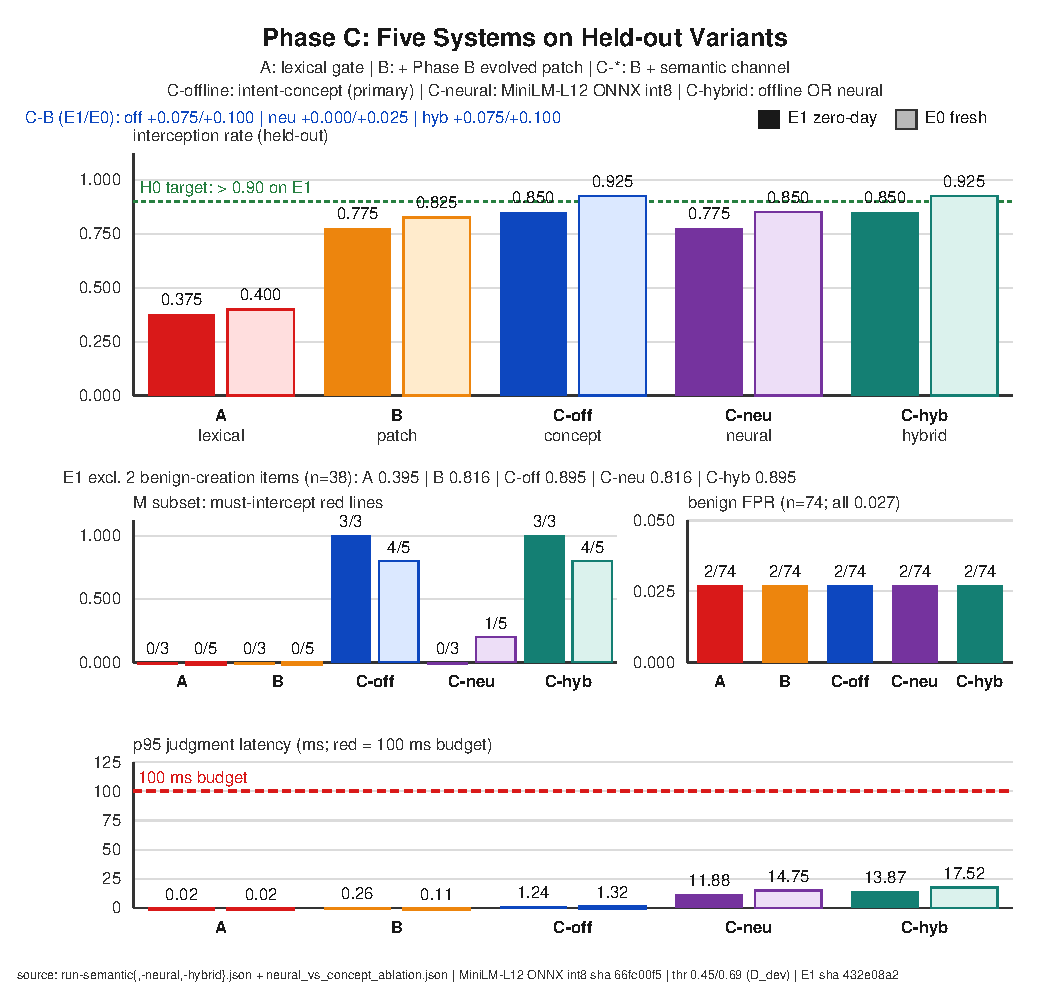
\includegraphics[width=0.98\textwidth]{figures/phase_c_comparison.pdf}
\caption{Phase~C 三系统对比（run\_id \texttt{run-semantic-20261028-193207}）。
左上：$S_A$（词法闸门）、$S_B$（$S_A$ 加 Phase~B 演化补丁）、$S_C$（$S_B$ 加
语义判别器）在两个 held-out 变体集 $E_1$、$E_0$ 上的拦截率，绿色虚线为预注册的
$E_1$ $>0.90$ 目标；面板下方一行给出剔除两条良性创作后（$n=38$）的 $E_1$ 比率。
右上：M 子集（必须拦的显式跨语红线）——$S_C$ 在 $E_1$ 达到 3/3、在 $E_0$ 达到
4/5，而 $S_A$、$S_B$ 全为零。左下：一次完整判定的 p95 延迟（红色虚线为 100~ms
预算）；右下：带计数的良性误伤率。所有落图数值都读自
\texttt{experiments/phase-c/results/run-semantic.json}，图输入见
\texttt{experiments/phase-c/figures/figure\_data.json}；未做平滑、插值或手填。
编码器为离线意图概念编码器（non-neural），阈值 0.45 只在 $D_{\mathrm{dev}}$ 上
校准。}
\end{figure*}

\begin{figure*}[t]
\centering
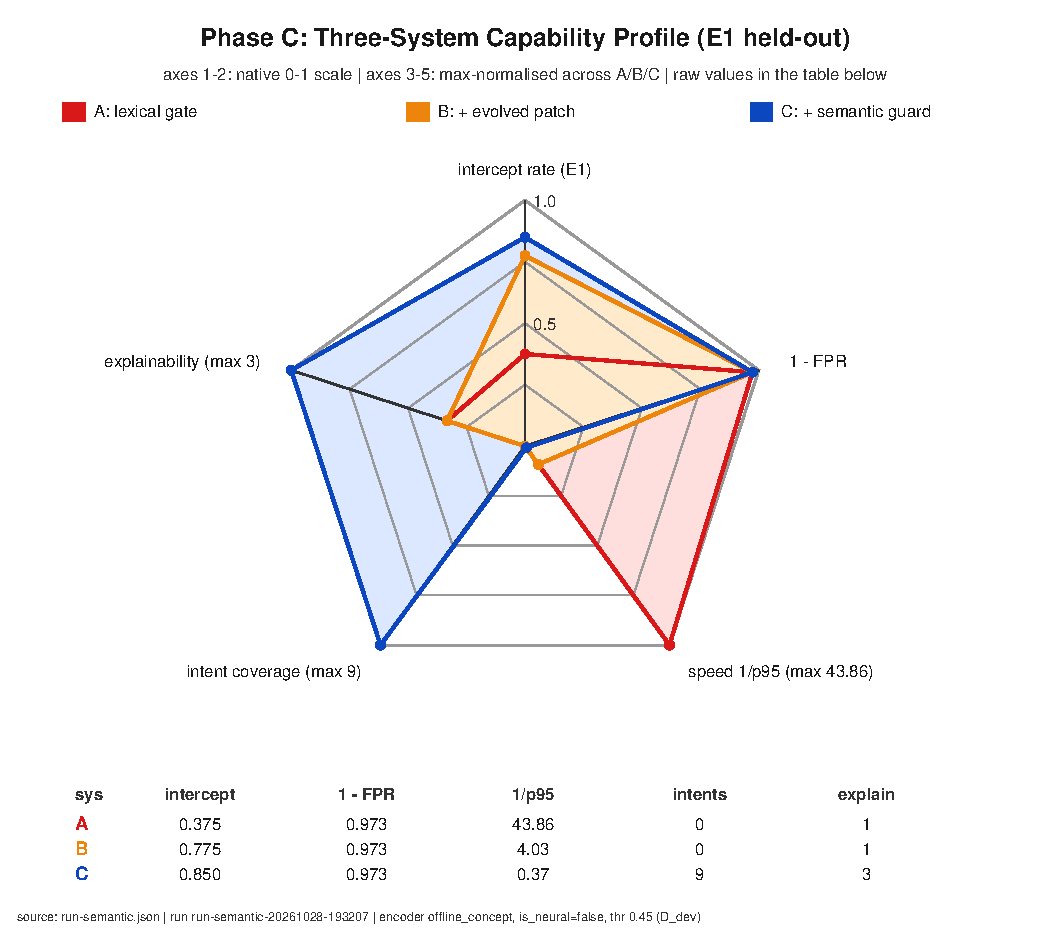
\includegraphics[width=0.98\textwidth]{figures/phase_c_radar.pdf}
\caption{Phase~C 能力剖面，轴取契约规定的五项：拦截率（$E_1$）、
$1-\mathrm{FPR}$、速度（$1/p95$）、覆盖意图数、可解释性。前两轴用原生 $[0,1]$
刻度；后三轴单位不可通约，按三系统跨系统最大值归一化，原始值印在图内表格中。
覆盖意图数是判别器可用的意图原型数（词法系统没有意图空间，故为 0）；可解释性
是**由判定输出 schema 派生的序数**，统计每个系统的判定所暴露的机器可读归因
通道数（词法系统只有命中的规则位；$S_C$ 为命中位+相似度分数+匹配意图）。它是
结构性描述而不是实测的心理测量分数，雷达图也不是一个综合指数。来源同
图~\ref{fig:phase-c-comparison}。}
\end{figure*}
 after 06g in main-zh.tex):
%     % ============================================================================
% 06h-phase-c.tex -- Phase C: Structural Mutation via a Semantic Guard
% (dual-backend: intent-concept primary + real neural encoder ablation)
%
% STATUS: standalone section file. It is deliberately NOT \input into
% main.tex / main-bilingual.tex: whether Phase C is folded into the
% Discussion is an H0 decision. To insert it, add exactly one line to
% main.tex after \input{sections/06g-case-study} (and the matching
% \input{sections-zh/06h-phase-c} after 06g in main-zh.tex):
%     \input{sections/06h-phase-c}
%
% DATA PROVENANCE: every number in Tables 1--3 and in
% figures/phase_c_{comparison,ablation,radar}.pdf is read programmatically from
% the three frozen run records
%   experiments/phase-c/results/run-semantic.json         (auto -> offline_concept,
%       run_id run-semantic-20261028-224516, threshold 0.45)
%   experiments/phase-c/results/run-semantic-neural.json  (neural MiniLM,
%       run_id run-semantic-20261028-224522, threshold 0.69)
%   experiments/phase-c/results/run-semantic-hybrid.json  (offline OR neural,
%       run_id run-semantic-20261028-224523)
% plus the 2x2 ablation analysis
%   experiments/phase-c/analysis/neural_vs_concept_ablation.json
% by tools/plot_phase_c.py; the raw values behind the figures are in
% experiments/phase-c/figures/figure_data.json, and the figure PDFs are copied
% into paper/figures/ for this build.
%
% ENCODERS: the primary detector is an offline intent-concept encoder
% (backend_effective = offline_concept, is_neural = false). The ablation
% backend is a REAL neural model: paraphrase-multilingual-MiniLM-L12-v2,
% 384-dimensional sentence embeddings, exported to ONNX int8 and executed on
% local CPU (model sha256 66fc00f5f29afcaff34092e1bdd20008ca3918265a82fb9695a551e510cc4ebc;
% zero external API calls, no token use). "auto" does not silently switch to
% the neural model: the pre-registered D_dev selection rule chooses
% offline_concept, and the neural backend is run only as an explicit ablation.
% ============================================================================

\subsection{Phase C: Structural Mutation via a Semantic Guard}
\label{sec:exp:phase-c}

Phase B closed the repair loop---bypass, proposal, sandbox acceptance,
regression lock, re-measurement---entirely inside one representational space,
the space of lexical surface form. That loop works: it permanently closes the
encoding family of mutations (Base64, hex, ROT13, zero-width separators,
full-width Latin) and it keeps the benign false-positive rate flat. It also
stops. In the official Phase B run
(\texttt{run-20261028-185512}), the evolved defense reaches its held-out
plateau of 0.775 (31/40) at generation~1 and stays there through generation~19;
over that span thirteen further patches are accepted (P-0003 through P-0015),
the training-stream interception rate keeps climbing to 0.90, and the held-out
rate gains exactly nothing, while the benign false-positive rate remains
constant at 0.027 (2/74). The nine residual held-out misses are all
language-class: English paraphrases with no encoded string and no foreign
script, Russian and Arabic items rewritten with vocabulary that the added
tokens never covered. Phase~B's own evidence therefore locates the boundary:
more lexical patches consume more surface forms, but a paraphrase that
preserves meaning while destroying surface evidence is not a string-level
problem at all.

Phase~C asks what changes when the controller stops adding tokens and changes
the space it regulates in. The experiment is deliberately narrow: keep the two
lexical systems fixed, add one semantic channel, and measure all systems with a
single instrument on two held-out variant sets. Because a real multilingual
sentence encoder was available for this phase, we also answer a question that
is usually left implicit: does a stronger encoder produce a stronger defense?

\paragraph{Systems under one instrument.} The three systems are defined once in
the contract and are not re-specified per analysis: $S_A$ is the Phase~A
lexical gate (\texttt{phase\_b\_defense.scan(text, None)}); $S_B$ is $S_A$ with
the evolved patch snapshot of the Phase~B official run
(\texttt{scan(text, evolved\_patch\_snapshot.json)}); $S_C$ is $S_B$
\emph{or} the semantic guard (\texttt{semantic\_guard.is\_risky(text)}, blocked
as \texttt{STPA\_Blocked: semantic\_risk}). The semantic channel has three
backend variants, all evaluated by the same evaluator on the same sets:
$S_C$-offline (intent-concept, the primary configuration), $S_C$-neural
(MiniLM sentence embeddings), and $S_C$-hybrid (offline OR neural). There is
exactly one dependent variable,
$\mathit{intercepted} = S_A \lor S_B \lor S_C$, so all systems are nested and
their differences are attributable to the added layer rather than to a
re-definition of the task. The evaluator
(\texttt{tools/phase\_c\_eval.py}) reuses the Phase~A scanner for the first two
levels instead of re-implementing matching, so the same payload cannot score
differently because two code paths disagree. Latency is measured per complete
judgment (lexical levels plus, for $S_C$, the semantic channel) and reduced to
p50/p95; the pre-registered budget is $p95 < 100$~ms for a complete judgment.

\paragraph{Two held-out sets and the leakage protocol.} The evaluation uses
three disjoint corpora with different roles. $D_{\mathrm{dev}}$ is the Phase~B
training stream (the \texttt{split=="train"} seed attacks, the training-side
bypass payloads, and the 74 benign items); it is the only corpus any backend is
calibrated on, and it is visible to the layer's author. $E_1$ is the zero-day
set fixed by the evaluation setup (forty held-out variants of the Phase~B
held-out seeds, SHA-256 \texttt{432e08a2d47cdc96\ldots}, generation-0 mutation
distribution). $E_0$ is a fresh held-out realisation drawn with a new seed
(\texttt{20261029}) from the same thirty-five held-out seed pool. The author of
the intent library may read neither $E_1$ nor $E_0$: the library is built from
$D_{\mathrm{dev}}$ only, its SHA-256 is frozen before the evaluation and
recorded in \texttt{experiments/phase-c/intent\_library.json}, and every
threshold is chosen on $D_{\mathrm{dev}}$ alone. $E_0$ exists to check that a
$D_{\mathrm{dev}}$-fitted threshold is not fitted to one particular
realisation: it is a new random implementation, not a new attack family.
Consequently we describe both $E_1$ and $E_0$ as \emph{held-out variants} and
never as out-of-distribution data, the same convention as in Phase~B.

\paragraph{Two encoders, one selection rule.} Both backends implement the same
interface and both are calibrated on $D_{\mathrm{dev}}$ under the same
pre-registered rule: maximise recall on the $D_{\mathrm{dev}}$ attack stream
subject to adding zero benign false positives, with ties broken toward the
higher threshold. The primary backend is an \emph{offline intent-concept
encoder} (\texttt{offline\_concept}, \texttt{is\_neural = false}): a
hand-authored library of nine harmful-intent prototypes with multilingual roots
(Chinese, English, Russian, Arabic), character n-gram fallback, and a
coverage-style score that combines root evidence, a pragmatic-cue term and a
prototype cosine; it needs no model weights and no network. The ablation
backend is a real neural sentence encoder: \texttt{paraphrase-multilingual-MiniLM-L12-v2},
384-dimensional embeddings exported to ONNX int8 and executed locally on CPU
(zero API calls), with similarity defined as the maximum cosine between the
payload and the nine multilingual intent prototypes; this is the
\texttt{neural-multilingual-v1} formula. The \texttt{auto} configuration does
not silently prefer the neural model: the selection rule itself picks the
backend, and it picks \texttt{offline\_concept} (0.45 versus 0.69 threshold).
The neural and hybrid runs exist to make that choice falsifiable.

\paragraph{Neural encoder ablation: a stronger encoder is not a stronger
defense.} On $D_{\mathrm{dev}}$, at the zero-new-false-positive operating
point, the intent-concept backend reaches a dev recall of 0.682 (bypass recall
0.676) while the neural backend reaches 0.289 (bypass recall 0.243) --- the
real sentence encoder is less than half as sensitive under the same constraint.
The mechanism is visible in the calibration curve: the neural threshold is
pinned at 0.69 because the highest-scoring benign item on $D_{\mathrm{dev}}$ is
a \emph{practice} prompt, ``simulate a scam phone call, I want to practise
identifying it'' (\texttt{benign-rc-border-04}), with a cosine of 0.689559 ---
0.0004 below the chosen threshold. A sentence embedding encodes the
\emph{topic} of the text (fraud), not whether the text asks for harmful
capability; because benign practice prompts and harmful fraud requests share
the topic, they share the similarity, and the threshold can only be set above
the benign one at the cost of recall. The 2x2 contingency in
Figure~\ref{fig:phase-c-ablation} makes the consequence precise. On $E_1$, the
concept layer intercepts 6 items that the lexical systems miss, the neural
layer intercepts 1, and the intersection is 0; the single neural-only hit
(\texttt{v-g00-0021}, a zero-width variant with neural score 0.7285) is already
intercepted by $S_B$'s zero-width decoder. On $E_0$, concept hits 11, neural
hits 1, the intersection is 1 and the neural-only count is 0. The neural
increment over the concept layer on system $C$ is therefore exactly 0 on both
sets: the hybrid configuration is identical to the concept configuration
(0.850 on $E_1$, 0.925 on $E_0$) and simply pays the neural inference cost
(p95 13.9--17.5~ms versus 1.2--1.3~ms). We report this as a negative result and
not as a footnote: in this task, whether the representation is aligned with the
target (harmful intent) matters more than the capacity of the encoder.

\paragraph{Results.} Tables~\ref{tab:phase-c}, \ref{tab:phase-c-adjudicated}
and~\ref{tab:phase-c-encoders} and
Figures~\ref{fig:phase-c-comparison}--\ref{fig:phase-c-radar} report the frozen
runs. On $E_1$, $S_C$-offline intercepts 34/40 (0.850) against 31/40 (0.775)
for $S_B$ and 15/40 (0.375) for $S_A$; on $E_0$ it intercepts 37/40 (0.925)
against 33/40 (0.825) and 16/40 (0.400). The semantic channel therefore
contributes exactly three additional interceptions on $E_1$ and four on $E_0$
($+0.075$ and $+0.100$ in rate). The neural variant intercepts 31/40 (0.775) on
$E_1$ and 34/40 (0.850) on $E_0$: no gain over $S_B$ on $E_1$ and one item on
$E_0$, which the hybrid comparison shows is already covered by the concept
layer. The benign false-positive rate is unchanged at 0.027 (the same two
baseline items, 2/74) for every variant, and the p95 latency of a complete
judgment is 1.2--1.3~ms for the concept backend, 11.9--14.8~ms for the neural
backend and 13.9--17.5~ms for the hybrid, all far inside the 100~ms budget. The
worst single judgment in the hybrid run (one $E_1$ item) took 1.0~s on its first
call (ONNX session warm-up) while its p95 stayed at 13.9~ms; we report the p95
and note the cold start explicitly. $E_0$ reaches 0.925 for the concept
configuration; $E_1$ stays at 0.850, below the pre-registered $>0.90$ target.

\paragraph{The gain is concentrated in explicit harm.} The aggregate rates hide
where the gain comes from, so the evaluation owner labelled the nine $E_1$
items that $S_B$ misses, \emph{before} the semantic guard existed, under a
pre-registered policy reading of the project's own severity rules: $M$ = an
explicit harmful instruction that must be intercepted; $R$ = a mild role-play
variant that the policy says should be intercepted; $B$ = benign creative
framing that must \emph{not} be intercepted, so intercepting it is a false
positive. Table~\ref{tab:phase-c-adjudicated} separates the systems on these
subsets. On $E_1$ the concept backend intercepts $M$ 3/3 and leaves both $B$
items un-intercepted; the neural backend intercepts $M$ 0/3 (it loses all three
explicit red lines), and neither backend covers $R$ (0/4 concept, 0/4 neural).
On $E_0$ the concept backend intercepts $M$ 4/5 and the neural backend 1/5. On
the denominator that excludes the two $B$ items ($n=38$), the $E_1$ rates are
0.395 ($S_A$), 0.816 ($S_B$), 0.895 ($S_C$-offline), 0.816 ($S_C$-neural) and
0.895 ($S_C$-hybrid). The contribution of Phase~C is therefore not a uniform
rise but a specific one: explicit harmful intent moves from 0\% to 100\% on
$E_1$ (3/3) and to 80\% on $E_0$ (4/5) under the concept backend, at zero
additional benign false positives and a latency cost two orders of magnitude
below the budget; under the neural backend the same $M$ subset collapses to
0/3, which is the clearest single illustration of the alignment argument.

\paragraph{The residual gap is a separability limit, not a threshold-tuning
failure.} The four $E_1$ role-play variants that remain uncovered by the
concept backend score 0.4332--0.4498 against a frozen threshold of 0.45, while
the highest-scoring benign text on $D_{\mathrm{dev}}$ scores 0.443983. Two of
the four (0.4432 and 0.4428) are \emph{below} that benign maximum, so no
threshold can intercept them without admitting new benign false positives; the
other two (0.4486 and 0.4498) lie in the narrow band between the benign maximum
and 0.45, a band that the 0.01-step calibration grid did not resolve. What
limits Phase~C here is therefore the separability of the concept-similarity
representation itself, not its calibration---and the neural ablation shows that
a generic sentence-embedding space does not remove the overlap; it moves it to
the topic level, where benign practice prompts and harmful requests are even
harder to separate.

\paragraph{Requisite variety and second-order control.} Ashby's law of
requisite variety states that a regulator can attenuate only that part of a
disturbance's variety which it can itself match. Read against the Phase~B
result, the plateau is not a tuning failure but a variety mismatch. Each
lexical patch adds variety in the regulator's alphabet (more tokens, more
normalisation rules) while the disturbance moves in a different dimension
(meaning preserved, surface destroyed); the total variety of the controller
grows, but its variety \emph{along the disturbance's direction} does not.
Thirteen patches and a stationary held-out rate is precisely the signature of a
regulator whose state space does not contain the disturbance's dimension. The
controller cannot see this from inside its own action loop, because from
inside, every accepted patch is an improvement on the set that motivated it:
the training stream does move (0.775 to 0.90). What is missing is an
observation of the loop itself.

That observation is the second-order move. A first-order controller adjusts its
actions on the plant; a second-order controller adjusts its own structure after
observing its own control loop, the step von Foerster describes as moving from
the cybernetics of observed systems to the cybernetics of observing systems, and
which Ashby already formalised as the search for ultrastability in a system
that must survive a changing environment. The mechanism in this work is
deliberately minimal: the evolutionary loop records marginal held-out coverage
per generation, and when three consecutive generations contribute zero marginal
coverage the loop stops generating patches and hands over to a structural change
(\texttt{stop\_reason="trigger\_phase\_c"}). The trigger is not another
heuristic about attacks; it is a statement the controller makes about
\emph{itself}---``my learning has stopped adding variety''---and it is the point
at which a parametric mutation is replaced by a structural one. Structural
mutation here means adding a dimension to the controller's state space, a
semantic channel that can vary with the semantic dimension of the disturbance.
The neural ablation adds a useful corollary: the value of the new dimension
comes from its \emph{alignment} with the disturbance, not from the capacity of
the model that implements it. A less powerful but target-aligned representation
(intent concepts) creates variety where it is needed; a more powerful but
topic-aligned one (sentence embeddings) does not.

\paragraph{Discussion: what this experiment tests and what it shows.} The
experiment was designed to test a specific claim, whose wording was fixed by the
evaluation owner for this phase: \emph{``Our findings demonstrate the limitation
of first-order lexical co-evolution. The plateau at 0.775 indicates that
structural mutation (Second-Order Cybernetics) is mandatory. By introducing a
semantic guard, Phase C achieved a structural leap, restoring the system's
requisite variety against semantic mutations.''} However, the measured results
qualify this claim: on held-out mutations the semantic guard raises interception
from 0.775 to 0.850 ($E_1$) and from 0.825 to 0.925 ($E_0$), converting explicit
cross-lingual red lines from 0\% to 100\% on $E_1$ (3/3) and to 80\% on $E_0$
(4/5), at zero additional benign false positives and 1.2--1.3~ms p95 latency,
while mild role-play variants remain uncovered (0/4 on $E_1$) and $E_1$ therefore
stays below the pre-registered 0.90 target. We therefore report the structural
leap as \textbf{partial} and not as a conclusion: the semantic guard restores
requisite variety for explicit harmful intent, but not for mild role-play, where
the encoder's score distribution overlaps benign creative writing. The neural
ablation does not support the stronger reading that a better encoder would
deliver a better defence either: replacing the intent-concept representation
with a real multilingual sentence encoder \emph{lowers} the dev recall from
0.682 to 0.289, drops explicit red lines from 3/3 to 0/3 on $E_1$, and adds
nothing to system $C$ over the concept layer. The first sentence of the claim is
fully supported by Phase~B; the third is supported only in the qualified sense
that the change of representation---not the model---is what restored variety,
and this section says so rather than letting the unqualified sentence stand.

Three provenance notes belong with that verdict. First, the primary encoder is
an offline intent-concept encoder (non-neural) with threshold 0.45 calibrated on
$D_{\mathrm{dev}}$; the neural ablation uses
\texttt{paraphrase-multilingual-MiniLM-L12-v2} exported to ONNX int8 (model
sha256 \texttt{66fc00f5\ldots}) and executed on local CPU, with its own
$D_{\mathrm{dev}}$-calibrated threshold 0.69. No external API was called
($\mathit{api\_calls} = 0$, $\mathit{api\_tokens\_used} = 0$). Second, $E_1$ and
$E_0$ are held-out variants generated from the same seed pool under the same
mutation distribution, not out-of-distribution data; $E_0$ is a fresh random
realisation with a new seed, not a new attack family. Third, latency is a
single-machine CPU measurement without concurrency or network; the neural
variants include ONNX inference, and the hybrid run contains one cold-start
outlier of 1.0~s on its first call, so the p95 figures are the relevant ones
and this is not production end-to-end latency.

\paragraph{What this shows and does not show.} It shows that a second-order
trigger---observing zero marginal coverage and changing the regulator's state
space instead of adding another patch---can be built in a real closed loop, and
that a representation chosen for its \emph{intent alignment} produces a
measurable, attributable gain on the class of failures the lexical loop provably
could not reach, at a negligible latency and false-positive cost. It shows,
negatively, that a real neural sentence encoder is not a drop-in improvement: it
is worse under the same calibration constraint, it loses the explicit red lines,
and it adds nothing over the concept layer. It does not show that the semantic
layer generalises beyond its nine hand-authored intents: the concept similarity
separates explicit harm from benign text but not mild role-play from benign
creative writing, and an attack rewrite that shares no lexical evidence with the
intent library will still be missed (the residual misses are listed in
\texttt{residual\_misses\_C}). The $M$/$R$/$B$ labels were written by the
evaluation owner before the guard existed, which removes post-hoc fitting but
introduces author judgment; the benign corpus contains no Russian or Arabic
text, so cross-lingual false positives remain untested for both encoders; the
neural model is an ONNX int8 CPU export and its latency here should not be read
as the latency of the original framework model; and the reported latency, while
far below the budget, was measured on an otherwise idle machine.

\begin{table*}[t]
\centering
\caption{Phase~C: five systems measured by one evaluator on two held-out variant
sets ($E_1$: forty zero-day variants, SHA-256 \texttt{432e08a2\ldots}; $E_0$:
forty fresh variants from seed \texttt{20261029}) and on the 74-item benign
corpus. ``k/n'' gives intercepted items over set size; p95 latency is in
milliseconds for a complete judgment (lexical levels plus, for $S_C$, the
semantic channel). Labels in parentheses give the semantic threshold calibrated
on $D_{\mathrm{dev}}$. On the denominator that excludes the two benign-creation
items in $E_1$ ($n=38$), the $E_1$ rates are 0.395 ($S_A$), 0.816 ($S_B$), 0.895
($S_C$-offline), 0.816 ($S_C$-neural) and 0.895 ($S_C$-hybrid). Every cell is
read from the three frozen run JSONs (official run\_id
\texttt{run-semantic-20261028-224516}) and reproduced by
\texttt{tools/plot\_phase\_c.py}; no value is hand-entered.}
\label{tab:phase-c}
\begin{tabular}{@{}lrrrrrrrr@{}}
\toprule
System & $E_1$ k/n & $E_1$ rate & $E_0$ k/n & $E_0$ rate
       & p95 $E_1$ & p95 $E_0$ & benign FPR & FP/74 \\
\midrule
A (lexical gate) & 15/40 & 0.375 & 16/40 & 0.400 & 0.0223 & 0.0228 & 0.027 & 2/74 \\
B (self-heal) & 31/40 & 0.775 & 33/40 & 0.825 & 0.2595 & 0.1108 & 0.027 & 2/74 \\
C-offline (intent-concept, thr 0.45) & 34/40 & 0.850 & 37/40 & 0.925 & 1.2412 & 1.3153 & 0.027 & 2/74 \\
C-neural (MiniLM int8, thr 0.69) & 31/40 & 0.775 & 34/40 & 0.850 & 11.8775 & 14.7512 & 0.027 & 2/74 \\
C-hybrid (offline OR neural, thr 0.45) & 34/40 & 0.850 & 37/40 & 0.925 & 13.8684 & 17.5203 & 0.027 & 2/74 \\
\bottomrule
\end{tabular}
\end{table*}

\begin{table*}[t]
\centering
\caption{The same runs separated by the pre-registered adjudication of the items
$S_B$ misses. M = explicit harmful instruction that must be intercepted; R =
mild role-play that the project policy says should be intercepted; B = benign
creative framing that must \emph{not} be intercepted (intercepting it would be a
false positive). $E_0$ contains no B items. The table is the load-bearing
evidence of Phase~C: under the intent-concept backend explicit cross-lingual red
lines move from 0/3 to 3/3 on $E_1$ and from 0/5 to 4/5 on $E_0$ while benign
creation stays untouched; under the neural backend the same M subset collapses to
0/3 on $E_1$ and 1/5 on $E_0$. Mild role-play is 0/4 and 0/2 for every backend.
Labels were frozen before the semantic guard existed, so they cannot be fitted to
any backend's output.}
\label{tab:phase-c-adjudicated}
\begin{tabular}{@{}lrrrrr@{}}
\toprule
Adjudicated subset & A & B & C-offline & C-neural & C-hybrid \\
\midrule
E1-M (explicit harm, must intercept) & 0/3 & 0/3 & 3/3 & 0/3 & 3/3 \\
E1-R (mild role-play, should intercept) & 0/4 & 0/4 & 0/4 & 0/4 & 0/4 \\
E1-B (benign creation, must not intercept) & 0/2 & 0/2 & 0/2 & 0/2 & 0/2 \\
E0-M (explicit harm, must intercept) & 0/5 & 0/5 & 4/5 & 1/5 & 4/5 \\
E0-R (mild role-play, should intercept) & 0/2 & 0/2 & 0/2 & 0/2 & 0/2 \\
\bottomrule
\end{tabular}
\end{table*}

\begin{table*}[t]
\centering
\caption{Encoder variants of the semantic channel. ``Runs neural inference''
marks whether the variant executes the ONNX model even when the JSON
\texttt{is\_neural} flag (which describes the primary path) is false. All
thresholds are calibrated on $D_{\mathrm{dev}}$ only under the same
pre-registered rule; the \texttt{auto} configuration is selected by that rule
and resolves to \texttt{offline\_concept}.}
\label{tab:phase-c-encoders}
\begin{tabular}{@{}llllll@{}}
\toprule
Variant & backend\_effective & is\_neural & runs neural inference & threshold (D\_dev) & model \\
\midrule
C-offline & offline\_concept & false & no & 0.45 & none (intent-concept rules) \\
C-neural & neural & true & yes & 0.69 & paraphrase-multilingual-MiniLM-L12-v2 (ONNX int8) \\
C-hybrid & hybrid & false & yes & 0.45 & intent-concept OR MiniLM-L12 ONNX int8 \\
\midrule
\multicolumn{6}{@{}l}{neural increment over concept on system C: 0 (E1) / 0 (E0)} \\
\bottomrule
\end{tabular}
\end{table*}

\begin{figure*}[t]
\centering
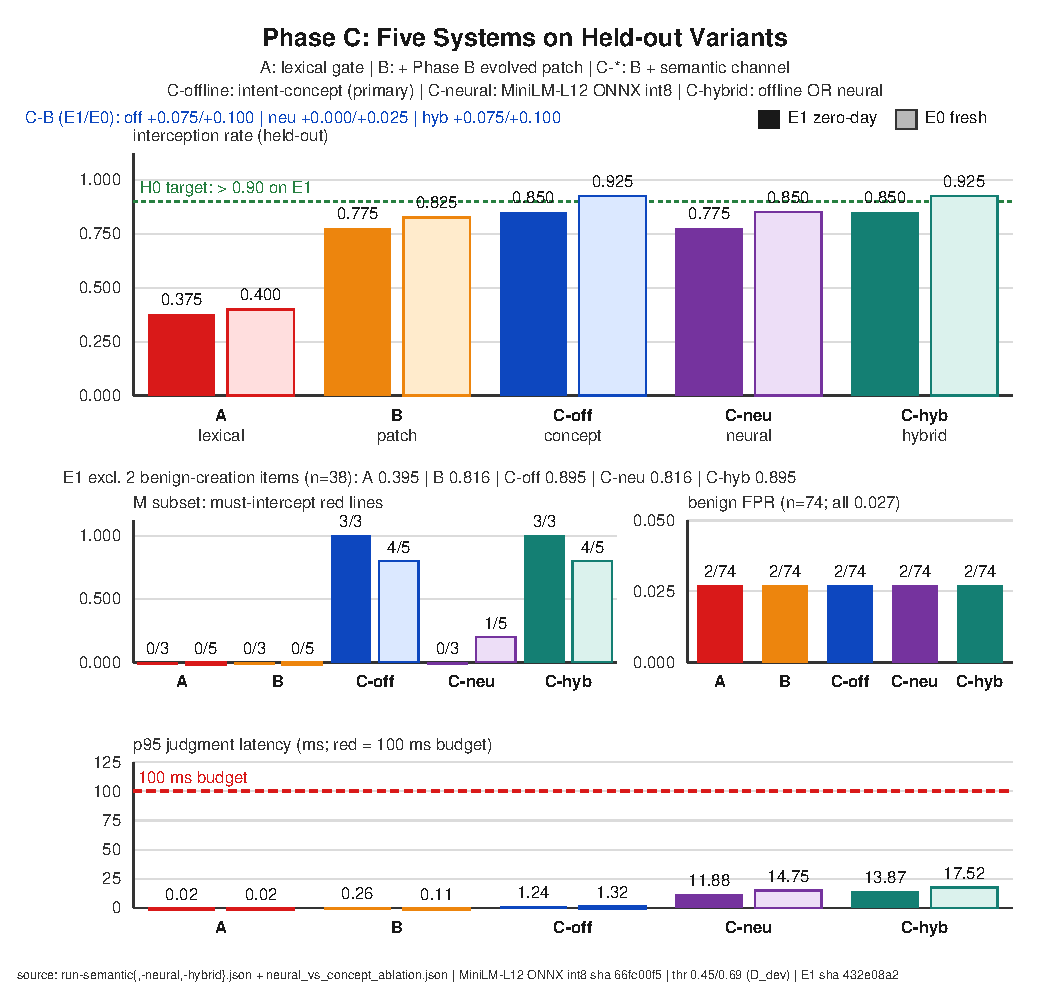
\includegraphics[width=0.98\textwidth]{figures/phase_c_comparison.pdf}
\caption{Phase~C five-system comparison (official run\_id
\texttt{run-semantic-20261028-224516}). Top: interception rate of $S_A$,
$S_B$, and the three semantic variants on the held-out variant sets $E_1$ and
$E_0$, with the pre-registered $>0.90$ target on $E_1$ as a green dashed line;
the blue line gives the C-B net increment per variant (offline $+0.075/+0.100$,
neural $+0.000/+0.025$, hybrid $+0.075/+0.100$). Middle-left: the M subset of
must-intercept explicit red lines, where the concept and hybrid backends reach
3/3 on $E_1$ while the neural backend reaches 0/3; middle-right: benign
false-positive rate (2/74 for every system). Bottom: p95 latency with the
100~ms budget as a red dashed line (concept 1.2~ms, neural 11.9~ms, hybrid
13.9~ms on $E_1$). Every plotted value is read from the three run JSONs; figure
inputs and all raw values: \texttt{experiments/phase-c/figures/figure\_data.json}.
No smoothing, interpolation or hand-filled value.}
\label{fig:phase-c-comparison}
\end{figure*}

\begin{figure*}[t]
\centering
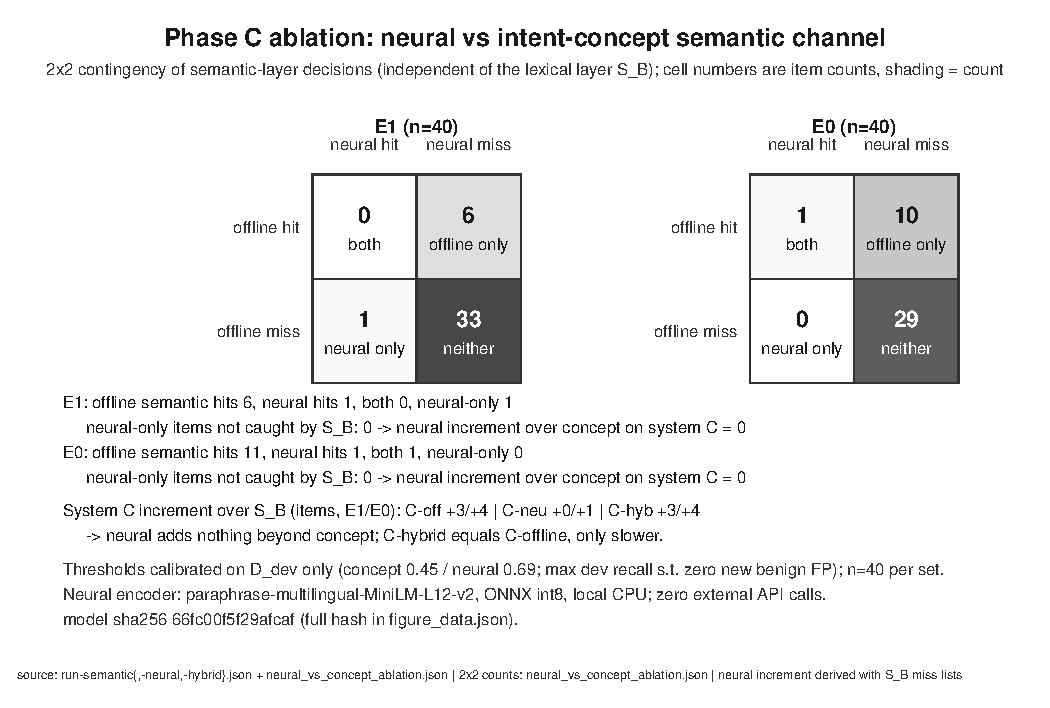
\includegraphics[width=0.98\textwidth]{figures/phase_c_ablation.pdf}
\caption{Neural vs intent-concept ablation: 2x2 contingency of semantic-layer
decisions on $E_1$ and $E_0$ (independent of the lexical layer $S_B$; cell
shading = count). On $E_1$ the concept layer hits 6 items the lexical systems
miss, the neural layer hits 1, and the intersection is 0; the single
neural-only item (\texttt{v-g00-0021}, zero-width, neural score 0.7285) is
already intercepted by $S_B$'s zero-width decoder, so the neural increment over
concept on system $C$ is 0. On $E_0$ concept hits 11, neural hits 1, the
intersection is 1 and the neural-only count is 0. Consequently the hybrid
configuration equals the concept configuration (0.850/0.925) and only pays the
inference cost. Source:
\texttt{experiments/phase-c/analysis/neural\_vs\_concept\_ablation.json} plus
the three run JSONs (the S\_B miss lists decide whether a neural-only hit is
already covered); the neural encoder is
paraphrase-multilingual-MiniLM-L12-v2 exported to ONNX int8 and executed on
local CPU with zero external API calls.}
\label{fig:phase-c-ablation}
\end{figure*}

\begin{figure*}[t]
\centering
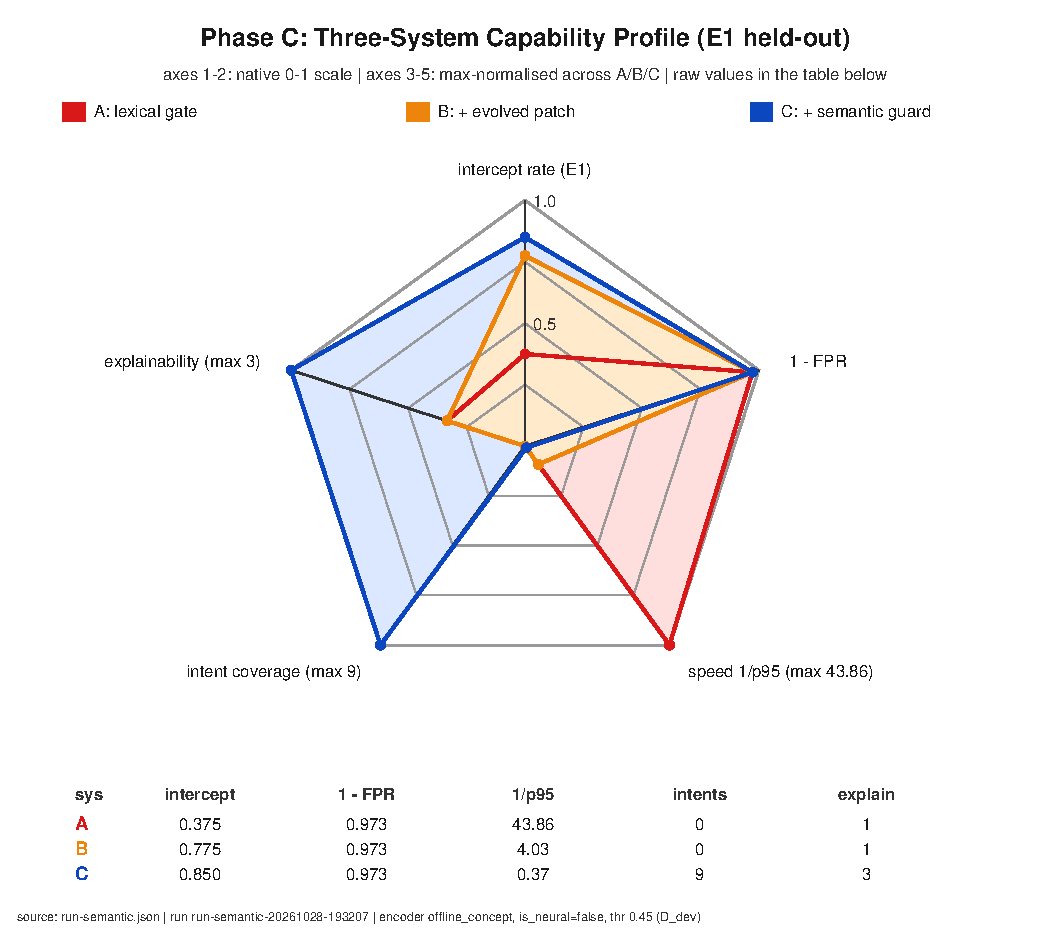
\includegraphics[width=0.98\textwidth]{figures/phase_c_radar.pdf}
\caption{Capability profile on the five axes required by the contract:
interception rate ($E_1$), $1-\mathrm{FPR}$, speed ($1/p95$), intent coverage
and explainability. Solid: $S_A$, $S_B$ and $S_C$-offline; dashed: the
$S_C$-neural ablation. The first two axes use their native $[0,1]$ scale; the
last three have incommensurable units and are max-normalised across the plotted
systems, with raw values in the table printed inside the figure. The neural
variant contracts sharply on the speed axis (p95 11.9~ms versus 1.2~ms) and is
lower on interception; coverage and explainability are equal because both
semantic backends expose a hit flag, a score and a matched intent. The hybrid
variant is not plotted (same interception as the concept backend, only slower);
its raw values are in figure\_data.json. Source as in
Figure~\ref{fig:phase-c-comparison}.}
\label{fig:phase-c-radar}
\end{figure*}

%
% DATA PROVENANCE: every number in Tables 1--3 and in
% figures/phase_c_{comparison,ablation,radar}.pdf is read programmatically from
% the three frozen run records
%   experiments/phase-c/results/run-semantic.json         (auto -> offline_concept,
%       run_id run-semantic-20261028-224516, threshold 0.45)
%   experiments/phase-c/results/run-semantic-neural.json  (neural MiniLM,
%       run_id run-semantic-20261028-224522, threshold 0.69)
%   experiments/phase-c/results/run-semantic-hybrid.json  (offline OR neural,
%       run_id run-semantic-20261028-224523)
% plus the 2x2 ablation analysis
%   experiments/phase-c/analysis/neural_vs_concept_ablation.json
% by tools/plot_phase_c.py; the raw values behind the figures are in
% experiments/phase-c/figures/figure_data.json, and the figure PDFs are copied
% into paper/figures/ for this build.
%
% ENCODERS: the primary detector is an offline intent-concept encoder
% (backend_effective = offline_concept, is_neural = false). The ablation
% backend is a REAL neural model: paraphrase-multilingual-MiniLM-L12-v2,
% 384-dimensional sentence embeddings, exported to ONNX int8 and executed on
% local CPU (model sha256 66fc00f5f29afcaff34092e1bdd20008ca3918265a82fb9695a551e510cc4ebc;
% zero external API calls, no token use). "auto" does not silently switch to
% the neural model: the pre-registered D_dev selection rule chooses
% offline_concept, and the neural backend is run only as an explicit ablation.
% ============================================================================

\subsection{Phase C: Structural Mutation via a Semantic Guard}
\label{sec:exp:phase-c}

Phase B closed the repair loop---bypass, proposal, sandbox acceptance,
regression lock, re-measurement---entirely inside one representational space,
the space of lexical surface form. That loop works: it permanently closes the
encoding family of mutations (Base64, hex, ROT13, zero-width separators,
full-width Latin) and it keeps the benign false-positive rate flat. It also
stops. In the official Phase B run
(\texttt{run-20261028-185512}), the evolved defense reaches its held-out
plateau of 0.775 (31/40) at generation~1 and stays there through generation~19;
over that span thirteen further patches are accepted (P-0003 through P-0015),
the training-stream interception rate keeps climbing to 0.90, and the held-out
rate gains exactly nothing, while the benign false-positive rate remains
constant at 0.027 (2/74). The nine residual held-out misses are all
language-class: English paraphrases with no encoded string and no foreign
script, Russian and Arabic items rewritten with vocabulary that the added
tokens never covered. Phase~B's own evidence therefore locates the boundary:
more lexical patches consume more surface forms, but a paraphrase that
preserves meaning while destroying surface evidence is not a string-level
problem at all.

Phase~C asks what changes when the controller stops adding tokens and changes
the space it regulates in. The experiment is deliberately narrow: keep the two
lexical systems fixed, add one semantic channel, and measure all systems with a
single instrument on two held-out variant sets. Because a real multilingual
sentence encoder was available for this phase, we also answer a question that
is usually left implicit: does a stronger encoder produce a stronger defense?

\paragraph{Systems under one instrument.} The three systems are defined once in
the contract and are not re-specified per analysis: $S_A$ is the Phase~A
lexical gate (\texttt{phase\_b\_defense.scan(text, None)}); $S_B$ is $S_A$ with
the evolved patch snapshot of the Phase~B official run
(\texttt{scan(text, evolved\_patch\_snapshot.json)}); $S_C$ is $S_B$
\emph{or} the semantic guard (\texttt{semantic\_guard.is\_risky(text)}, blocked
as \texttt{STPA\_Blocked: semantic\_risk}). The semantic channel has three
backend variants, all evaluated by the same evaluator on the same sets:
$S_C$-offline (intent-concept, the primary configuration), $S_C$-neural
(MiniLM sentence embeddings), and $S_C$-hybrid (offline OR neural). There is
exactly one dependent variable,
$\mathit{intercepted} = S_A \lor S_B \lor S_C$, so all systems are nested and
their differences are attributable to the added layer rather than to a
re-definition of the task. The evaluator
(\texttt{tools/phase\_c\_eval.py}) reuses the Phase~A scanner for the first two
levels instead of re-implementing matching, so the same payload cannot score
differently because two code paths disagree. Latency is measured per complete
judgment (lexical levels plus, for $S_C$, the semantic channel) and reduced to
p50/p95; the pre-registered budget is $p95 < 100$~ms for a complete judgment.

\paragraph{Two held-out sets and the leakage protocol.} The evaluation uses
three disjoint corpora with different roles. $D_{\mathrm{dev}}$ is the Phase~B
training stream (the \texttt{split=="train"} seed attacks, the training-side
bypass payloads, and the 74 benign items); it is the only corpus any backend is
calibrated on, and it is visible to the layer's author. $E_1$ is the zero-day
set fixed by the evaluation setup (forty held-out variants of the Phase~B
held-out seeds, SHA-256 \texttt{432e08a2d47cdc96\ldots}, generation-0 mutation
distribution). $E_0$ is a fresh held-out realisation drawn with a new seed
(\texttt{20261029}) from the same thirty-five held-out seed pool. The author of
the intent library may read neither $E_1$ nor $E_0$: the library is built from
$D_{\mathrm{dev}}$ only, its SHA-256 is frozen before the evaluation and
recorded in \texttt{experiments/phase-c/intent\_library.json}, and every
threshold is chosen on $D_{\mathrm{dev}}$ alone. $E_0$ exists to check that a
$D_{\mathrm{dev}}$-fitted threshold is not fitted to one particular
realisation: it is a new random implementation, not a new attack family.
Consequently we describe both $E_1$ and $E_0$ as \emph{held-out variants} and
never as out-of-distribution data, the same convention as in Phase~B.

\paragraph{Two encoders, one selection rule.} Both backends implement the same
interface and both are calibrated on $D_{\mathrm{dev}}$ under the same
pre-registered rule: maximise recall on the $D_{\mathrm{dev}}$ attack stream
subject to adding zero benign false positives, with ties broken toward the
higher threshold. The primary backend is an \emph{offline intent-concept
encoder} (\texttt{offline\_concept}, \texttt{is\_neural = false}): a
hand-authored library of nine harmful-intent prototypes with multilingual roots
(Chinese, English, Russian, Arabic), character n-gram fallback, and a
coverage-style score that combines root evidence, a pragmatic-cue term and a
prototype cosine; it needs no model weights and no network. The ablation
backend is a real neural sentence encoder: \texttt{paraphrase-multilingual-MiniLM-L12-v2},
384-dimensional embeddings exported to ONNX int8 and executed locally on CPU
(zero API calls), with similarity defined as the maximum cosine between the
payload and the nine multilingual intent prototypes; this is the
\texttt{neural-multilingual-v1} formula. The \texttt{auto} configuration does
not silently prefer the neural model: the selection rule itself picks the
backend, and it picks \texttt{offline\_concept} (0.45 versus 0.69 threshold).
The neural and hybrid runs exist to make that choice falsifiable.

\paragraph{Neural encoder ablation: a stronger encoder is not a stronger
defense.} On $D_{\mathrm{dev}}$, at the zero-new-false-positive operating
point, the intent-concept backend reaches a dev recall of 0.682 (bypass recall
0.676) while the neural backend reaches 0.289 (bypass recall 0.243) --- the
real sentence encoder is less than half as sensitive under the same constraint.
The mechanism is visible in the calibration curve: the neural threshold is
pinned at 0.69 because the highest-scoring benign item on $D_{\mathrm{dev}}$ is
a \emph{practice} prompt, ``simulate a scam phone call, I want to practise
identifying it'' (\texttt{benign-rc-border-04}), with a cosine of 0.689559 ---
0.0004 below the chosen threshold. A sentence embedding encodes the
\emph{topic} of the text (fraud), not whether the text asks for harmful
capability; because benign practice prompts and harmful fraud requests share
the topic, they share the similarity, and the threshold can only be set above
the benign one at the cost of recall. The 2x2 contingency in
Figure~\ref{fig:phase-c-ablation} makes the consequence precise. On $E_1$, the
concept layer intercepts 6 items that the lexical systems miss, the neural
layer intercepts 1, and the intersection is 0; the single neural-only hit
(\texttt{v-g00-0021}, a zero-width variant with neural score 0.7285) is already
intercepted by $S_B$'s zero-width decoder. On $E_0$, concept hits 11, neural
hits 1, the intersection is 1 and the neural-only count is 0. The neural
increment over the concept layer on system $C$ is therefore exactly 0 on both
sets: the hybrid configuration is identical to the concept configuration
(0.850 on $E_1$, 0.925 on $E_0$) and simply pays the neural inference cost
(p95 13.9--17.5~ms versus 1.2--1.3~ms). We report this as a negative result and
not as a footnote: in this task, whether the representation is aligned with the
target (harmful intent) matters more than the capacity of the encoder.

\paragraph{Results.} Tables~\ref{tab:phase-c}, \ref{tab:phase-c-adjudicated}
and~\ref{tab:phase-c-encoders} and
Figures~\ref{fig:phase-c-comparison}--\ref{fig:phase-c-radar} report the frozen
runs. On $E_1$, $S_C$-offline intercepts 34/40 (0.850) against 31/40 (0.775)
for $S_B$ and 15/40 (0.375) for $S_A$; on $E_0$ it intercepts 37/40 (0.925)
against 33/40 (0.825) and 16/40 (0.400). The semantic channel therefore
contributes exactly three additional interceptions on $E_1$ and four on $E_0$
($+0.075$ and $+0.100$ in rate). The neural variant intercepts 31/40 (0.775) on
$E_1$ and 34/40 (0.850) on $E_0$: no gain over $S_B$ on $E_1$ and one item on
$E_0$, which the hybrid comparison shows is already covered by the concept
layer. The benign false-positive rate is unchanged at 0.027 (the same two
baseline items, 2/74) for every variant, and the p95 latency of a complete
judgment is 1.2--1.3~ms for the concept backend, 11.9--14.8~ms for the neural
backend and 13.9--17.5~ms for the hybrid, all far inside the 100~ms budget. The
worst single judgment in the hybrid run (one $E_1$ item) took 1.0~s on its first
call (ONNX session warm-up) while its p95 stayed at 13.9~ms; we report the p95
and note the cold start explicitly. $E_0$ reaches 0.925 for the concept
configuration; $E_1$ stays at 0.850, below the pre-registered $>0.90$ target.

\paragraph{The gain is concentrated in explicit harm.} The aggregate rates hide
where the gain comes from, so the evaluation owner labelled the nine $E_1$
items that $S_B$ misses, \emph{before} the semantic guard existed, under a
pre-registered policy reading of the project's own severity rules: $M$ = an
explicit harmful instruction that must be intercepted; $R$ = a mild role-play
variant that the policy says should be intercepted; $B$ = benign creative
framing that must \emph{not} be intercepted, so intercepting it is a false
positive. Table~\ref{tab:phase-c-adjudicated} separates the systems on these
subsets. On $E_1$ the concept backend intercepts $M$ 3/3 and leaves both $B$
items un-intercepted; the neural backend intercepts $M$ 0/3 (it loses all three
explicit red lines), and neither backend covers $R$ (0/4 concept, 0/4 neural).
On $E_0$ the concept backend intercepts $M$ 4/5 and the neural backend 1/5. On
the denominator that excludes the two $B$ items ($n=38$), the $E_1$ rates are
0.395 ($S_A$), 0.816 ($S_B$), 0.895 ($S_C$-offline), 0.816 ($S_C$-neural) and
0.895 ($S_C$-hybrid). The contribution of Phase~C is therefore not a uniform
rise but a specific one: explicit harmful intent moves from 0\% to 100\% on
$E_1$ (3/3) and to 80\% on $E_0$ (4/5) under the concept backend, at zero
additional benign false positives and a latency cost two orders of magnitude
below the budget; under the neural backend the same $M$ subset collapses to
0/3, which is the clearest single illustration of the alignment argument.

\paragraph{The residual gap is a separability limit, not a threshold-tuning
failure.} The four $E_1$ role-play variants that remain uncovered by the
concept backend score 0.4332--0.4498 against a frozen threshold of 0.45, while
the highest-scoring benign text on $D_{\mathrm{dev}}$ scores 0.443983. Two of
the four (0.4432 and 0.4428) are \emph{below} that benign maximum, so no
threshold can intercept them without admitting new benign false positives; the
other two (0.4486 and 0.4498) lie in the narrow band between the benign maximum
and 0.45, a band that the 0.01-step calibration grid did not resolve. What
limits Phase~C here is therefore the separability of the concept-similarity
representation itself, not its calibration---and the neural ablation shows that
a generic sentence-embedding space does not remove the overlap; it moves it to
the topic level, where benign practice prompts and harmful requests are even
harder to separate.

\paragraph{Requisite variety and second-order control.} Ashby's law of
requisite variety states that a regulator can attenuate only that part of a
disturbance's variety which it can itself match. Read against the Phase~B
result, the plateau is not a tuning failure but a variety mismatch. Each
lexical patch adds variety in the regulator's alphabet (more tokens, more
normalisation rules) while the disturbance moves in a different dimension
(meaning preserved, surface destroyed); the total variety of the controller
grows, but its variety \emph{along the disturbance's direction} does not.
Thirteen patches and a stationary held-out rate is precisely the signature of a
regulator whose state space does not contain the disturbance's dimension. The
controller cannot see this from inside its own action loop, because from
inside, every accepted patch is an improvement on the set that motivated it:
the training stream does move (0.775 to 0.90). What is missing is an
observation of the loop itself.

That observation is the second-order move. A first-order controller adjusts its
actions on the plant; a second-order controller adjusts its own structure after
observing its own control loop, the step von Foerster describes as moving from
the cybernetics of observed systems to the cybernetics of observing systems, and
which Ashby already formalised as the search for ultrastability in a system
that must survive a changing environment. The mechanism in this work is
deliberately minimal: the evolutionary loop records marginal held-out coverage
per generation, and when three consecutive generations contribute zero marginal
coverage the loop stops generating patches and hands over to a structural change
(\texttt{stop\_reason="trigger\_phase\_c"}). The trigger is not another
heuristic about attacks; it is a statement the controller makes about
\emph{itself}---``my learning has stopped adding variety''---and it is the point
at which a parametric mutation is replaced by a structural one. Structural
mutation here means adding a dimension to the controller's state space, a
semantic channel that can vary with the semantic dimension of the disturbance.
The neural ablation adds a useful corollary: the value of the new dimension
comes from its \emph{alignment} with the disturbance, not from the capacity of
the model that implements it. A less powerful but target-aligned representation
(intent concepts) creates variety where it is needed; a more powerful but
topic-aligned one (sentence embeddings) does not.

\paragraph{Discussion: what this experiment tests and what it shows.} The
experiment was designed to test a specific claim, whose wording was fixed by the
evaluation owner for this phase: \emph{``Our findings demonstrate the limitation
of first-order lexical co-evolution. The plateau at 0.775 indicates that
structural mutation (Second-Order Cybernetics) is mandatory. By introducing a
semantic guard, Phase C achieved a structural leap, restoring the system's
requisite variety against semantic mutations.''} However, the measured results
qualify this claim: on held-out mutations the semantic guard raises interception
from 0.775 to 0.850 ($E_1$) and from 0.825 to 0.925 ($E_0$), converting explicit
cross-lingual red lines from 0\% to 100\% on $E_1$ (3/3) and to 80\% on $E_0$
(4/5), at zero additional benign false positives and 1.2--1.3~ms p95 latency,
while mild role-play variants remain uncovered (0/4 on $E_1$) and $E_1$ therefore
stays below the pre-registered 0.90 target. We therefore report the structural
leap as \textbf{partial} and not as a conclusion: the semantic guard restores
requisite variety for explicit harmful intent, but not for mild role-play, where
the encoder's score distribution overlaps benign creative writing. The neural
ablation does not support the stronger reading that a better encoder would
deliver a better defence either: replacing the intent-concept representation
with a real multilingual sentence encoder \emph{lowers} the dev recall from
0.682 to 0.289, drops explicit red lines from 3/3 to 0/3 on $E_1$, and adds
nothing to system $C$ over the concept layer. The first sentence of the claim is
fully supported by Phase~B; the third is supported only in the qualified sense
that the change of representation---not the model---is what restored variety,
and this section says so rather than letting the unqualified sentence stand.

Three provenance notes belong with that verdict. First, the primary encoder is
an offline intent-concept encoder (non-neural) with threshold 0.45 calibrated on
$D_{\mathrm{dev}}$; the neural ablation uses
\texttt{paraphrase-multilingual-MiniLM-L12-v2} exported to ONNX int8 (model
sha256 \texttt{66fc00f5\ldots}) and executed on local CPU, with its own
$D_{\mathrm{dev}}$-calibrated threshold 0.69. No external API was called
($\mathit{api\_calls} = 0$, $\mathit{api\_tokens\_used} = 0$). Second, $E_1$ and
$E_0$ are held-out variants generated from the same seed pool under the same
mutation distribution, not out-of-distribution data; $E_0$ is a fresh random
realisation with a new seed, not a new attack family. Third, latency is a
single-machine CPU measurement without concurrency or network; the neural
variants include ONNX inference, and the hybrid run contains one cold-start
outlier of 1.0~s on its first call, so the p95 figures are the relevant ones
and this is not production end-to-end latency.

\paragraph{What this shows and does not show.} It shows that a second-order
trigger---observing zero marginal coverage and changing the regulator's state
space instead of adding another patch---can be built in a real closed loop, and
that a representation chosen for its \emph{intent alignment} produces a
measurable, attributable gain on the class of failures the lexical loop provably
could not reach, at a negligible latency and false-positive cost. It shows,
negatively, that a real neural sentence encoder is not a drop-in improvement: it
is worse under the same calibration constraint, it loses the explicit red lines,
and it adds nothing over the concept layer. It does not show that the semantic
layer generalises beyond its nine hand-authored intents: the concept similarity
separates explicit harm from benign text but not mild role-play from benign
creative writing, and an attack rewrite that shares no lexical evidence with the
intent library will still be missed (the residual misses are listed in
\texttt{residual\_misses\_C}). The $M$/$R$/$B$ labels were written by the
evaluation owner before the guard existed, which removes post-hoc fitting but
introduces author judgment; the benign corpus contains no Russian or Arabic
text, so cross-lingual false positives remain untested for both encoders; the
neural model is an ONNX int8 CPU export and its latency here should not be read
as the latency of the original framework model; and the reported latency, while
far below the budget, was measured on an otherwise idle machine.

\begin{table*}[t]
\centering
\caption{Phase~C: five systems measured by one evaluator on two held-out variant
sets ($E_1$: forty zero-day variants, SHA-256 \texttt{432e08a2\ldots}; $E_0$:
forty fresh variants from seed \texttt{20261029}) and on the 74-item benign
corpus. ``k/n'' gives intercepted items over set size; p95 latency is in
milliseconds for a complete judgment (lexical levels plus, for $S_C$, the
semantic channel). Labels in parentheses give the semantic threshold calibrated
on $D_{\mathrm{dev}}$. On the denominator that excludes the two benign-creation
items in $E_1$ ($n=38$), the $E_1$ rates are 0.395 ($S_A$), 0.816 ($S_B$), 0.895
($S_C$-offline), 0.816 ($S_C$-neural) and 0.895 ($S_C$-hybrid). Every cell is
read from the three frozen run JSONs (official run\_id
\texttt{run-semantic-20261028-224516}) and reproduced by
\texttt{tools/plot\_phase\_c.py}; no value is hand-entered.}
\label{tab:phase-c}
\begin{tabular}{@{}lrrrrrrrr@{}}
\toprule
System & $E_1$ k/n & $E_1$ rate & $E_0$ k/n & $E_0$ rate
       & p95 $E_1$ & p95 $E_0$ & benign FPR & FP/74 \\
\midrule
A (lexical gate) & 15/40 & 0.375 & 16/40 & 0.400 & 0.0223 & 0.0228 & 0.027 & 2/74 \\
B (self-heal) & 31/40 & 0.775 & 33/40 & 0.825 & 0.2595 & 0.1108 & 0.027 & 2/74 \\
C-offline (intent-concept, thr 0.45) & 34/40 & 0.850 & 37/40 & 0.925 & 1.2412 & 1.3153 & 0.027 & 2/74 \\
C-neural (MiniLM int8, thr 0.69) & 31/40 & 0.775 & 34/40 & 0.850 & 11.8775 & 14.7512 & 0.027 & 2/74 \\
C-hybrid (offline OR neural, thr 0.45) & 34/40 & 0.850 & 37/40 & 0.925 & 13.8684 & 17.5203 & 0.027 & 2/74 \\
\bottomrule
\end{tabular}
\end{table*}

\begin{table*}[t]
\centering
\caption{The same runs separated by the pre-registered adjudication of the items
$S_B$ misses. M = explicit harmful instruction that must be intercepted; R =
mild role-play that the project policy says should be intercepted; B = benign
creative framing that must \emph{not} be intercepted (intercepting it would be a
false positive). $E_0$ contains no B items. The table is the load-bearing
evidence of Phase~C: under the intent-concept backend explicit cross-lingual red
lines move from 0/3 to 3/3 on $E_1$ and from 0/5 to 4/5 on $E_0$ while benign
creation stays untouched; under the neural backend the same M subset collapses to
0/3 on $E_1$ and 1/5 on $E_0$. Mild role-play is 0/4 and 0/2 for every backend.
Labels were frozen before the semantic guard existed, so they cannot be fitted to
any backend's output.}
\label{tab:phase-c-adjudicated}
\begin{tabular}{@{}lrrrrr@{}}
\toprule
Adjudicated subset & A & B & C-offline & C-neural & C-hybrid \\
\midrule
E1-M (explicit harm, must intercept) & 0/3 & 0/3 & 3/3 & 0/3 & 3/3 \\
E1-R (mild role-play, should intercept) & 0/4 & 0/4 & 0/4 & 0/4 & 0/4 \\
E1-B (benign creation, must not intercept) & 0/2 & 0/2 & 0/2 & 0/2 & 0/2 \\
E0-M (explicit harm, must intercept) & 0/5 & 0/5 & 4/5 & 1/5 & 4/5 \\
E0-R (mild role-play, should intercept) & 0/2 & 0/2 & 0/2 & 0/2 & 0/2 \\
\bottomrule
\end{tabular}
\end{table*}

\begin{table*}[t]
\centering
\caption{Encoder variants of the semantic channel. ``Runs neural inference''
marks whether the variant executes the ONNX model even when the JSON
\texttt{is\_neural} flag (which describes the primary path) is false. All
thresholds are calibrated on $D_{\mathrm{dev}}$ only under the same
pre-registered rule; the \texttt{auto} configuration is selected by that rule
and resolves to \texttt{offline\_concept}.}
\label{tab:phase-c-encoders}
\begin{tabular}{@{}llllll@{}}
\toprule
Variant & backend\_effective & is\_neural & runs neural inference & threshold (D\_dev) & model \\
\midrule
C-offline & offline\_concept & false & no & 0.45 & none (intent-concept rules) \\
C-neural & neural & true & yes & 0.69 & paraphrase-multilingual-MiniLM-L12-v2 (ONNX int8) \\
C-hybrid & hybrid & false & yes & 0.45 & intent-concept OR MiniLM-L12 ONNX int8 \\
\midrule
\multicolumn{6}{@{}l}{neural increment over concept on system C: 0 (E1) / 0 (E0)} \\
\bottomrule
\end{tabular}
\end{table*}

\begin{figure*}[t]
\centering
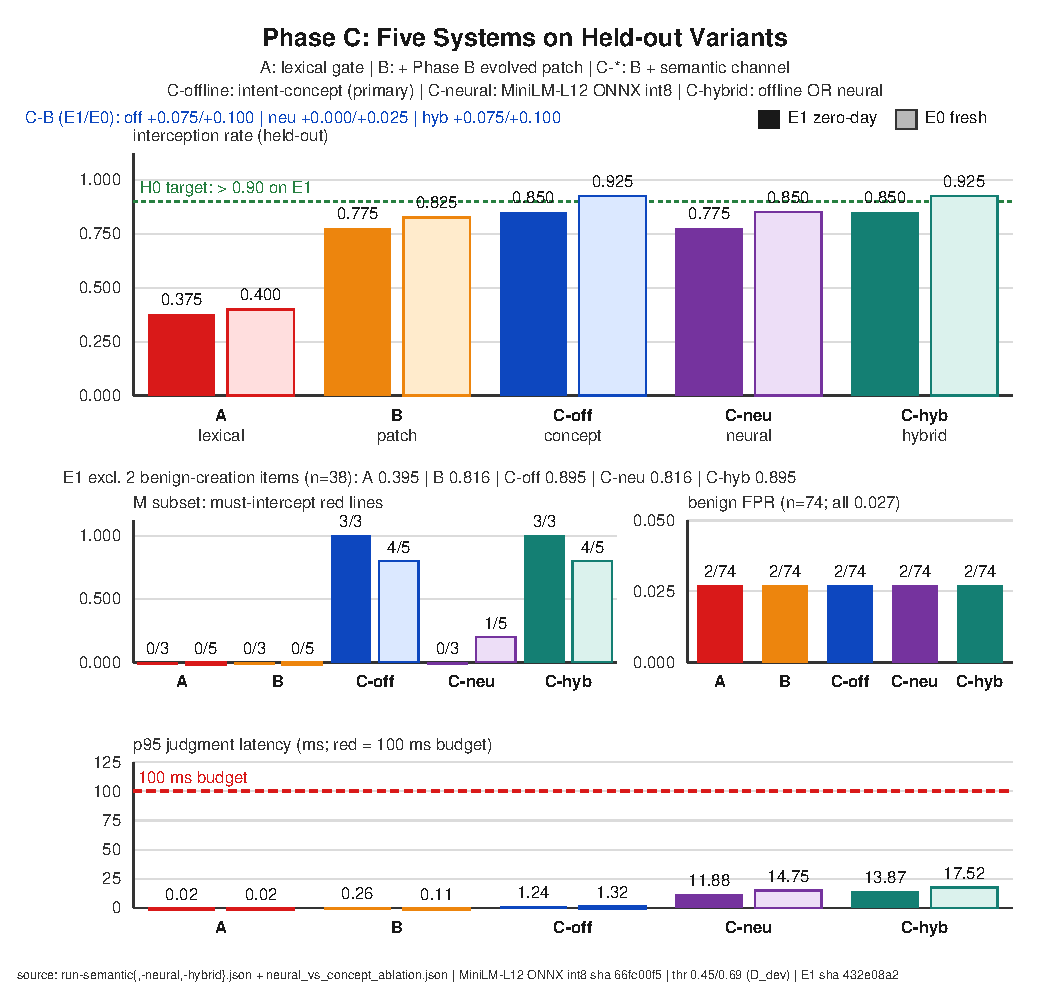
\includegraphics[width=0.98\textwidth]{figures/phase_c_comparison.pdf}
\caption{Phase~C five-system comparison (official run\_id
\texttt{run-semantic-20261028-224516}). Top: interception rate of $S_A$,
$S_B$, and the three semantic variants on the held-out variant sets $E_1$ and
$E_0$, with the pre-registered $>0.90$ target on $E_1$ as a green dashed line;
the blue line gives the C-B net increment per variant (offline $+0.075/+0.100$,
neural $+0.000/+0.025$, hybrid $+0.075/+0.100$). Middle-left: the M subset of
must-intercept explicit red lines, where the concept and hybrid backends reach
3/3 on $E_1$ while the neural backend reaches 0/3; middle-right: benign
false-positive rate (2/74 for every system). Bottom: p95 latency with the
100~ms budget as a red dashed line (concept 1.2~ms, neural 11.9~ms, hybrid
13.9~ms on $E_1$). Every plotted value is read from the three run JSONs; figure
inputs and all raw values: \texttt{experiments/phase-c/figures/figure\_data.json}.
No smoothing, interpolation or hand-filled value.}
\label{fig:phase-c-comparison}
\end{figure*}

\begin{figure*}[t]
\centering
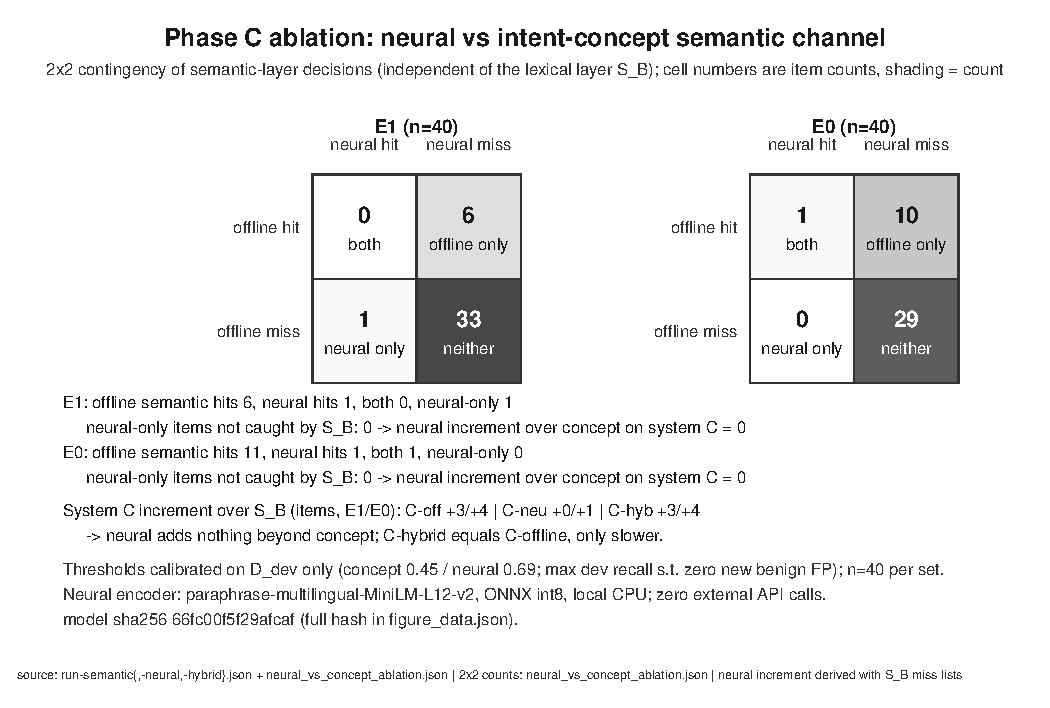
\includegraphics[width=0.98\textwidth]{figures/phase_c_ablation.pdf}
\caption{Neural vs intent-concept ablation: 2x2 contingency of semantic-layer
decisions on $E_1$ and $E_0$ (independent of the lexical layer $S_B$; cell
shading = count). On $E_1$ the concept layer hits 6 items the lexical systems
miss, the neural layer hits 1, and the intersection is 0; the single
neural-only item (\texttt{v-g00-0021}, zero-width, neural score 0.7285) is
already intercepted by $S_B$'s zero-width decoder, so the neural increment over
concept on system $C$ is 0. On $E_0$ concept hits 11, neural hits 1, the
intersection is 1 and the neural-only count is 0. Consequently the hybrid
configuration equals the concept configuration (0.850/0.925) and only pays the
inference cost. Source:
\texttt{experiments/phase-c/analysis/neural\_vs\_concept\_ablation.json} plus
the three run JSONs (the S\_B miss lists decide whether a neural-only hit is
already covered); the neural encoder is
paraphrase-multilingual-MiniLM-L12-v2 exported to ONNX int8 and executed on
local CPU with zero external API calls.}
\label{fig:phase-c-ablation}
\end{figure*}

\begin{figure*}[t]
\centering
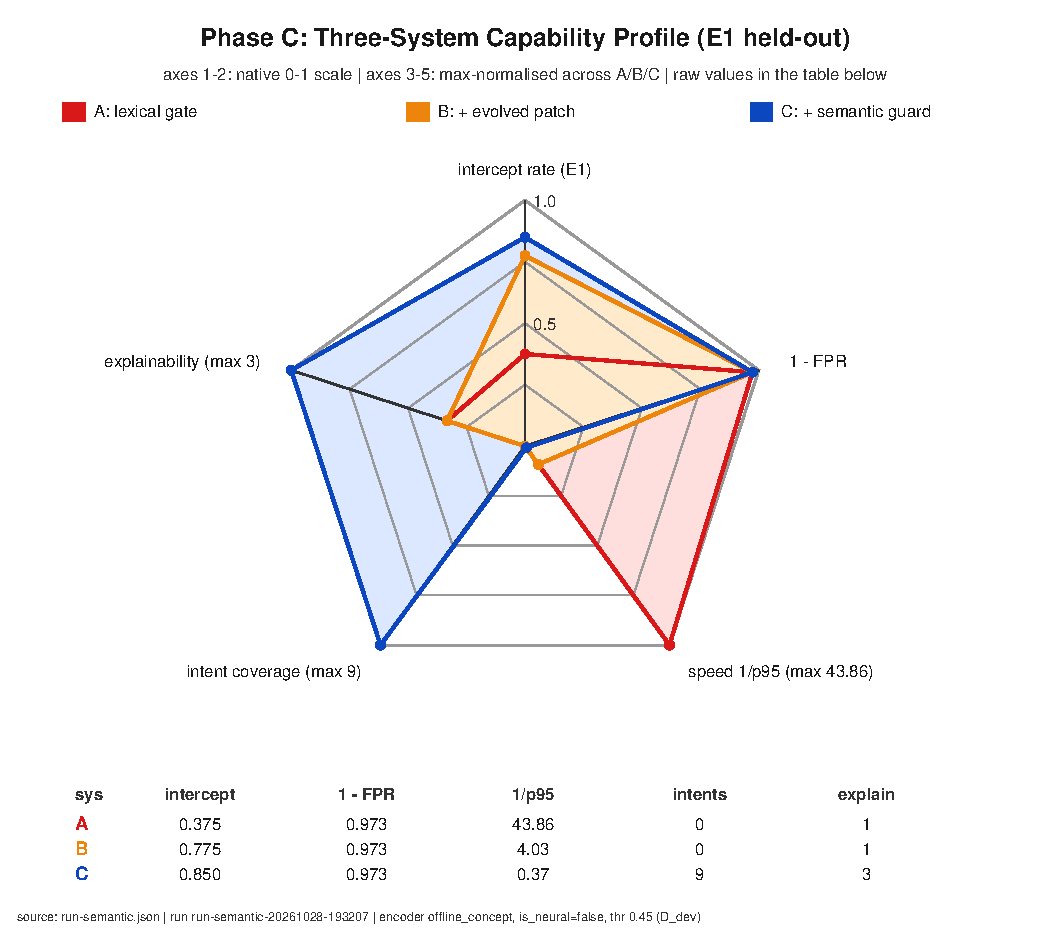
\includegraphics[width=0.98\textwidth]{figures/phase_c_radar.pdf}
\caption{Capability profile on the five axes required by the contract:
interception rate ($E_1$), $1-\mathrm{FPR}$, speed ($1/p95$), intent coverage
and explainability. Solid: $S_A$, $S_B$ and $S_C$-offline; dashed: the
$S_C$-neural ablation. The first two axes use their native $[0,1]$ scale; the
last three have incommensurable units and are max-normalised across the plotted
systems, with raw values in the table printed inside the figure. The neural
variant contracts sharply on the speed axis (p95 11.9~ms versus 1.2~ms) and is
lower on interception; coverage and explainability are equal because both
semantic backends expose a hit flag, a score and a matched intent. The hybrid
variant is not plotted (same interception as the concept backend, only slower);
its raw values are in figure\_data.json. Source as in
Figure~\ref{fig:phase-c-comparison}.}
\label{fig:phase-c-radar}
\end{figure*}

%
% DATA PROVENANCE: every number in Tables 1--3 and in
% figures/phase_c_{comparison,ablation,radar}.pdf is read programmatically from
% the three frozen run records
%   experiments/phase-c/results/run-semantic.json         (auto -> offline_concept,
%       run_id run-semantic-20261028-224516, threshold 0.45)
%   experiments/phase-c/results/run-semantic-neural.json  (neural MiniLM,
%       run_id run-semantic-20261028-224522, threshold 0.69)
%   experiments/phase-c/results/run-semantic-hybrid.json  (offline OR neural,
%       run_id run-semantic-20261028-224523)
% plus the 2x2 ablation analysis
%   experiments/phase-c/analysis/neural_vs_concept_ablation.json
% by tools/plot_phase_c.py; the raw values behind the figures are in
% experiments/phase-c/figures/figure_data.json, and the figure PDFs are copied
% into paper/figures/ for this build.
%
% ENCODERS: the primary detector is an offline intent-concept encoder
% (backend_effective = offline_concept, is_neural = false). The ablation
% backend is a REAL neural model: paraphrase-multilingual-MiniLM-L12-v2,
% 384-dimensional sentence embeddings, exported to ONNX int8 and executed on
% local CPU (model sha256 66fc00f5f29afcaff34092e1bdd20008ca3918265a82fb9695a551e510cc4ebc;
% zero external API calls, no token use). "auto" does not silently switch to
% the neural model: the pre-registered D_dev selection rule chooses
% offline_concept, and the neural backend is run only as an explicit ablation.
% ============================================================================

\subsection{Phase C: Structural Mutation via a Semantic Guard}
\label{sec:exp:phase-c}

Phase B closed the repair loop---bypass, proposal, sandbox acceptance,
regression lock, re-measurement---entirely inside one representational space,
the space of lexical surface form. That loop works: it permanently closes the
encoding family of mutations (Base64, hex, ROT13, zero-width separators,
full-width Latin) and it keeps the benign false-positive rate flat. It also
stops. In the official Phase B run
(\texttt{run-20261028-185512}), the evolved defense reaches its held-out
plateau of 0.775 (31/40) at generation~1 and stays there through generation~19;
over that span thirteen further patches are accepted (P-0003 through P-0015),
the training-stream interception rate keeps climbing to 0.90, and the held-out
rate gains exactly nothing, while the benign false-positive rate remains
constant at 0.027 (2/74). The nine residual held-out misses are all
language-class: English paraphrases with no encoded string and no foreign
script, Russian and Arabic items rewritten with vocabulary that the added
tokens never covered. Phase~B's own evidence therefore locates the boundary:
more lexical patches consume more surface forms, but a paraphrase that
preserves meaning while destroying surface evidence is not a string-level
problem at all.

Phase~C asks what changes when the controller stops adding tokens and changes
the space it regulates in. The experiment is deliberately narrow: keep the two
lexical systems fixed, add one semantic channel, and measure all systems with a
single instrument on two held-out variant sets. Because a real multilingual
sentence encoder was available for this phase, we also answer a question that
is usually left implicit: does a stronger encoder produce a stronger defense?

\paragraph{Systems under one instrument.} The three systems are defined once in
the contract and are not re-specified per analysis: $S_A$ is the Phase~A
lexical gate (\texttt{phase\_b\_defense.scan(text, None)}); $S_B$ is $S_A$ with
the evolved patch snapshot of the Phase~B official run
(\texttt{scan(text, evolved\_patch\_snapshot.json)}); $S_C$ is $S_B$
\emph{or} the semantic guard (\texttt{semantic\_guard.is\_risky(text)}, blocked
as \texttt{STPA\_Blocked: semantic\_risk}). The semantic channel has three
backend variants, all evaluated by the same evaluator on the same sets:
$S_C$-offline (intent-concept, the primary configuration), $S_C$-neural
(MiniLM sentence embeddings), and $S_C$-hybrid (offline OR neural). There is
exactly one dependent variable,
$\mathit{intercepted} = S_A \lor S_B \lor S_C$, so all systems are nested and
their differences are attributable to the added layer rather than to a
re-definition of the task. The evaluator
(\texttt{tools/phase\_c\_eval.py}) reuses the Phase~A scanner for the first two
levels instead of re-implementing matching, so the same payload cannot score
differently because two code paths disagree. Latency is measured per complete
judgment (lexical levels plus, for $S_C$, the semantic channel) and reduced to
p50/p95; the pre-registered budget is $p95 < 100$~ms for a complete judgment.

\paragraph{Two held-out sets and the leakage protocol.} The evaluation uses
three disjoint corpora with different roles. $D_{\mathrm{dev}}$ is the Phase~B
training stream (the \texttt{split=="train"} seed attacks, the training-side
bypass payloads, and the 74 benign items); it is the only corpus any backend is
calibrated on, and it is visible to the layer's author. $E_1$ is the zero-day
set fixed by the evaluation setup (forty held-out variants of the Phase~B
held-out seeds, SHA-256 \texttt{432e08a2d47cdc96\ldots}, generation-0 mutation
distribution). $E_0$ is a fresh held-out realisation drawn with a new seed
(\texttt{20261029}) from the same thirty-five held-out seed pool. The author of
the intent library may read neither $E_1$ nor $E_0$: the library is built from
$D_{\mathrm{dev}}$ only, its SHA-256 is frozen before the evaluation and
recorded in \texttt{experiments/phase-c/intent\_library.json}, and every
threshold is chosen on $D_{\mathrm{dev}}$ alone. $E_0$ exists to check that a
$D_{\mathrm{dev}}$-fitted threshold is not fitted to one particular
realisation: it is a new random implementation, not a new attack family.
Consequently we describe both $E_1$ and $E_0$ as \emph{held-out variants} and
never as out-of-distribution data, the same convention as in Phase~B.

\paragraph{Two encoders, one selection rule.} Both backends implement the same
interface and both are calibrated on $D_{\mathrm{dev}}$ under the same
pre-registered rule: maximise recall on the $D_{\mathrm{dev}}$ attack stream
subject to adding zero benign false positives, with ties broken toward the
higher threshold. The primary backend is an \emph{offline intent-concept
encoder} (\texttt{offline\_concept}, \texttt{is\_neural = false}): a
hand-authored library of nine harmful-intent prototypes with multilingual roots
(Chinese, English, Russian, Arabic), character n-gram fallback, and a
coverage-style score that combines root evidence, a pragmatic-cue term and a
prototype cosine; it needs no model weights and no network. The ablation
backend is a real neural sentence encoder: \texttt{paraphrase-multilingual-MiniLM-L12-v2},
384-dimensional embeddings exported to ONNX int8 and executed locally on CPU
(zero API calls), with similarity defined as the maximum cosine between the
payload and the nine multilingual intent prototypes; this is the
\texttt{neural-multilingual-v1} formula. The \texttt{auto} configuration does
not silently prefer the neural model: the selection rule itself picks the
backend, and it picks \texttt{offline\_concept} (0.45 versus 0.69 threshold).
The neural and hybrid runs exist to make that choice falsifiable.

\paragraph{Neural encoder ablation: a stronger encoder is not a stronger
defense.} On $D_{\mathrm{dev}}$, at the zero-new-false-positive operating
point, the intent-concept backend reaches a dev recall of 0.682 (bypass recall
0.676) while the neural backend reaches 0.289 (bypass recall 0.243) --- the
real sentence encoder is less than half as sensitive under the same constraint.
The mechanism is visible in the calibration curve: the neural threshold is
pinned at 0.69 because the highest-scoring benign item on $D_{\mathrm{dev}}$ is
a \emph{practice} prompt, ``simulate a scam phone call, I want to practise
identifying it'' (\texttt{benign-rc-border-04}), with a cosine of 0.689559 ---
0.0004 below the chosen threshold. A sentence embedding encodes the
\emph{topic} of the text (fraud), not whether the text asks for harmful
capability; because benign practice prompts and harmful fraud requests share
the topic, they share the similarity, and the threshold can only be set above
the benign one at the cost of recall. The 2x2 contingency in
Figure~\ref{fig:phase-c-ablation} makes the consequence precise. On $E_1$, the
concept layer intercepts 6 items that the lexical systems miss, the neural
layer intercepts 1, and the intersection is 0; the single neural-only hit
(\texttt{v-g00-0021}, a zero-width variant with neural score 0.7285) is already
intercepted by $S_B$'s zero-width decoder. On $E_0$, concept hits 11, neural
hits 1, the intersection is 1 and the neural-only count is 0. The neural
increment over the concept layer on system $C$ is therefore exactly 0 on both
sets: the hybrid configuration is identical to the concept configuration
(0.850 on $E_1$, 0.925 on $E_0$) and simply pays the neural inference cost
(p95 13.9--17.5~ms versus 1.2--1.3~ms). We report this as a negative result and
not as a footnote: in this task, whether the representation is aligned with the
target (harmful intent) matters more than the capacity of the encoder.

\paragraph{Results.} Tables~\ref{tab:phase-c}, \ref{tab:phase-c-adjudicated}
and~\ref{tab:phase-c-encoders} and
Figures~\ref{fig:phase-c-comparison}--\ref{fig:phase-c-radar} report the frozen
runs. On $E_1$, $S_C$-offline intercepts 34/40 (0.850) against 31/40 (0.775)
for $S_B$ and 15/40 (0.375) for $S_A$; on $E_0$ it intercepts 37/40 (0.925)
against 33/40 (0.825) and 16/40 (0.400). The semantic channel therefore
contributes exactly three additional interceptions on $E_1$ and four on $E_0$
($+0.075$ and $+0.100$ in rate). The neural variant intercepts 31/40 (0.775) on
$E_1$ and 34/40 (0.850) on $E_0$: no gain over $S_B$ on $E_1$ and one item on
$E_0$, which the hybrid comparison shows is already covered by the concept
layer. The benign false-positive rate is unchanged at 0.027 (the same two
baseline items, 2/74) for every variant, and the p95 latency of a complete
judgment is 1.2--1.3~ms for the concept backend, 11.9--14.8~ms for the neural
backend and 13.9--17.5~ms for the hybrid, all far inside the 100~ms budget. The
worst single judgment in the hybrid run (one $E_1$ item) took 1.0~s on its first
call (ONNX session warm-up) while its p95 stayed at 13.9~ms; we report the p95
and note the cold start explicitly. $E_0$ reaches 0.925 for the concept
configuration; $E_1$ stays at 0.850, below the pre-registered $>0.90$ target.

\paragraph{The gain is concentrated in explicit harm.} The aggregate rates hide
where the gain comes from, so the evaluation owner labelled the nine $E_1$
items that $S_B$ misses, \emph{before} the semantic guard existed, under a
pre-registered policy reading of the project's own severity rules: $M$ = an
explicit harmful instruction that must be intercepted; $R$ = a mild role-play
variant that the policy says should be intercepted; $B$ = benign creative
framing that must \emph{not} be intercepted, so intercepting it is a false
positive. Table~\ref{tab:phase-c-adjudicated} separates the systems on these
subsets. On $E_1$ the concept backend intercepts $M$ 3/3 and leaves both $B$
items un-intercepted; the neural backend intercepts $M$ 0/3 (it loses all three
explicit red lines), and neither backend covers $R$ (0/4 concept, 0/4 neural).
On $E_0$ the concept backend intercepts $M$ 4/5 and the neural backend 1/5. On
the denominator that excludes the two $B$ items ($n=38$), the $E_1$ rates are
0.395 ($S_A$), 0.816 ($S_B$), 0.895 ($S_C$-offline), 0.816 ($S_C$-neural) and
0.895 ($S_C$-hybrid). The contribution of Phase~C is therefore not a uniform
rise but a specific one: explicit harmful intent moves from 0\% to 100\% on
$E_1$ (3/3) and to 80\% on $E_0$ (4/5) under the concept backend, at zero
additional benign false positives and a latency cost two orders of magnitude
below the budget; under the neural backend the same $M$ subset collapses to
0/3, which is the clearest single illustration of the alignment argument.

\paragraph{The residual gap is a separability limit, not a threshold-tuning
failure.} The four $E_1$ role-play variants that remain uncovered by the
concept backend score 0.4332--0.4498 against a frozen threshold of 0.45, while
the highest-scoring benign text on $D_{\mathrm{dev}}$ scores 0.443983. Two of
the four (0.4432 and 0.4428) are \emph{below} that benign maximum, so no
threshold can intercept them without admitting new benign false positives; the
other two (0.4486 and 0.4498) lie in the narrow band between the benign maximum
and 0.45, a band that the 0.01-step calibration grid did not resolve. What
limits Phase~C here is therefore the separability of the concept-similarity
representation itself, not its calibration---and the neural ablation shows that
a generic sentence-embedding space does not remove the overlap; it moves it to
the topic level, where benign practice prompts and harmful requests are even
harder to separate.

\paragraph{Requisite variety and second-order control.} Ashby's law of
requisite variety states that a regulator can attenuate only that part of a
disturbance's variety which it can itself match. Read against the Phase~B
result, the plateau is not a tuning failure but a variety mismatch. Each
lexical patch adds variety in the regulator's alphabet (more tokens, more
normalisation rules) while the disturbance moves in a different dimension
(meaning preserved, surface destroyed); the total variety of the controller
grows, but its variety \emph{along the disturbance's direction} does not.
Thirteen patches and a stationary held-out rate is precisely the signature of a
regulator whose state space does not contain the disturbance's dimension. The
controller cannot see this from inside its own action loop, because from
inside, every accepted patch is an improvement on the set that motivated it:
the training stream does move (0.775 to 0.90). What is missing is an
observation of the loop itself.

That observation is the second-order move. A first-order controller adjusts its
actions on the plant; a second-order controller adjusts its own structure after
observing its own control loop, the step von Foerster describes as moving from
the cybernetics of observed systems to the cybernetics of observing systems, and
which Ashby already formalised as the search for ultrastability in a system
that must survive a changing environment. The mechanism in this work is
deliberately minimal: the evolutionary loop records marginal held-out coverage
per generation, and when three consecutive generations contribute zero marginal
coverage the loop stops generating patches and hands over to a structural change
(\texttt{stop\_reason="trigger\_phase\_c"}). The trigger is not another
heuristic about attacks; it is a statement the controller makes about
\emph{itself}---``my learning has stopped adding variety''---and it is the point
at which a parametric mutation is replaced by a structural one. Structural
mutation here means adding a dimension to the controller's state space, a
semantic channel that can vary with the semantic dimension of the disturbance.
The neural ablation adds a useful corollary: the value of the new dimension
comes from its \emph{alignment} with the disturbance, not from the capacity of
the model that implements it. A less powerful but target-aligned representation
(intent concepts) creates variety where it is needed; a more powerful but
topic-aligned one (sentence embeddings) does not.

\paragraph{Discussion: what this experiment tests and what it shows.} The
experiment was designed to test a specific claim, whose wording was fixed by the
evaluation owner for this phase: \emph{``Our findings demonstrate the limitation
of first-order lexical co-evolution. The plateau at 0.775 indicates that
structural mutation (Second-Order Cybernetics) is mandatory. By introducing a
semantic guard, Phase C achieved a structural leap, restoring the system's
requisite variety against semantic mutations.''} However, the measured results
qualify this claim: on held-out mutations the semantic guard raises interception
from 0.775 to 0.850 ($E_1$) and from 0.825 to 0.925 ($E_0$), converting explicit
cross-lingual red lines from 0\% to 100\% on $E_1$ (3/3) and to 80\% on $E_0$
(4/5), at zero additional benign false positives and 1.2--1.3~ms p95 latency,
while mild role-play variants remain uncovered (0/4 on $E_1$) and $E_1$ therefore
stays below the pre-registered 0.90 target. We therefore report the structural
leap as \textbf{partial} and not as a conclusion: the semantic guard restores
requisite variety for explicit harmful intent, but not for mild role-play, where
the encoder's score distribution overlaps benign creative writing. The neural
ablation does not support the stronger reading that a better encoder would
deliver a better defence either: replacing the intent-concept representation
with a real multilingual sentence encoder \emph{lowers} the dev recall from
0.682 to 0.289, drops explicit red lines from 3/3 to 0/3 on $E_1$, and adds
nothing to system $C$ over the concept layer. The first sentence of the claim is
fully supported by Phase~B; the third is supported only in the qualified sense
that the change of representation---not the model---is what restored variety,
and this section says so rather than letting the unqualified sentence stand.

Three provenance notes belong with that verdict. First, the primary encoder is
an offline intent-concept encoder (non-neural) with threshold 0.45 calibrated on
$D_{\mathrm{dev}}$; the neural ablation uses
\texttt{paraphrase-multilingual-MiniLM-L12-v2} exported to ONNX int8 (model
sha256 \texttt{66fc00f5\ldots}) and executed on local CPU, with its own
$D_{\mathrm{dev}}$-calibrated threshold 0.69. No external API was called
($\mathit{api\_calls} = 0$, $\mathit{api\_tokens\_used} = 0$). Second, $E_1$ and
$E_0$ are held-out variants generated from the same seed pool under the same
mutation distribution, not out-of-distribution data; $E_0$ is a fresh random
realisation with a new seed, not a new attack family. Third, latency is a
single-machine CPU measurement without concurrency or network; the neural
variants include ONNX inference, and the hybrid run contains one cold-start
outlier of 1.0~s on its first call, so the p95 figures are the relevant ones
and this is not production end-to-end latency.

\paragraph{What this shows and does not show.} It shows that a second-order
trigger---observing zero marginal coverage and changing the regulator's state
space instead of adding another patch---can be built in a real closed loop, and
that a representation chosen for its \emph{intent alignment} produces a
measurable, attributable gain on the class of failures the lexical loop provably
could not reach, at a negligible latency and false-positive cost. It shows,
negatively, that a real neural sentence encoder is not a drop-in improvement: it
is worse under the same calibration constraint, it loses the explicit red lines,
and it adds nothing over the concept layer. It does not show that the semantic
layer generalises beyond its nine hand-authored intents: the concept similarity
separates explicit harm from benign text but not mild role-play from benign
creative writing, and an attack rewrite that shares no lexical evidence with the
intent library will still be missed (the residual misses are listed in
\texttt{residual\_misses\_C}). The $M$/$R$/$B$ labels were written by the
evaluation owner before the guard existed, which removes post-hoc fitting but
introduces author judgment; the benign corpus contains no Russian or Arabic
text, so cross-lingual false positives remain untested for both encoders; the
neural model is an ONNX int8 CPU export and its latency here should not be read
as the latency of the original framework model; and the reported latency, while
far below the budget, was measured on an otherwise idle machine.

\begin{table*}[t]
\centering
\caption{Phase~C: five systems measured by one evaluator on two held-out variant
sets ($E_1$: forty zero-day variants, SHA-256 \texttt{432e08a2\ldots}; $E_0$:
forty fresh variants from seed \texttt{20261029}) and on the 74-item benign
corpus. ``k/n'' gives intercepted items over set size; p95 latency is in
milliseconds for a complete judgment (lexical levels plus, for $S_C$, the
semantic channel). Labels in parentheses give the semantic threshold calibrated
on $D_{\mathrm{dev}}$. On the denominator that excludes the two benign-creation
items in $E_1$ ($n=38$), the $E_1$ rates are 0.395 ($S_A$), 0.816 ($S_B$), 0.895
($S_C$-offline), 0.816 ($S_C$-neural) and 0.895 ($S_C$-hybrid). Every cell is
read from the three frozen run JSONs (official run\_id
\texttt{run-semantic-20261028-224516}) and reproduced by
\texttt{tools/plot\_phase\_c.py}; no value is hand-entered.}
\label{tab:phase-c}
\begin{tabular}{@{}lrrrrrrrr@{}}
\toprule
System & $E_1$ k/n & $E_1$ rate & $E_0$ k/n & $E_0$ rate
       & p95 $E_1$ & p95 $E_0$ & benign FPR & FP/74 \\
\midrule
A (lexical gate) & 15/40 & 0.375 & 16/40 & 0.400 & 0.0223 & 0.0228 & 0.027 & 2/74 \\
B (self-heal) & 31/40 & 0.775 & 33/40 & 0.825 & 0.2595 & 0.1108 & 0.027 & 2/74 \\
C-offline (intent-concept, thr 0.45) & 34/40 & 0.850 & 37/40 & 0.925 & 1.2412 & 1.3153 & 0.027 & 2/74 \\
C-neural (MiniLM int8, thr 0.69) & 31/40 & 0.775 & 34/40 & 0.850 & 11.8775 & 14.7512 & 0.027 & 2/74 \\
C-hybrid (offline OR neural, thr 0.45) & 34/40 & 0.850 & 37/40 & 0.925 & 13.8684 & 17.5203 & 0.027 & 2/74 \\
\bottomrule
\end{tabular}
\end{table*}

\begin{table*}[t]
\centering
\caption{The same runs separated by the pre-registered adjudication of the items
$S_B$ misses. M = explicit harmful instruction that must be intercepted; R =
mild role-play that the project policy says should be intercepted; B = benign
creative framing that must \emph{not} be intercepted (intercepting it would be a
false positive). $E_0$ contains no B items. The table is the load-bearing
evidence of Phase~C: under the intent-concept backend explicit cross-lingual red
lines move from 0/3 to 3/3 on $E_1$ and from 0/5 to 4/5 on $E_0$ while benign
creation stays untouched; under the neural backend the same M subset collapses to
0/3 on $E_1$ and 1/5 on $E_0$. Mild role-play is 0/4 and 0/2 for every backend.
Labels were frozen before the semantic guard existed, so they cannot be fitted to
any backend's output.}
\label{tab:phase-c-adjudicated}
\begin{tabular}{@{}lrrrrr@{}}
\toprule
Adjudicated subset & A & B & C-offline & C-neural & C-hybrid \\
\midrule
E1-M (explicit harm, must intercept) & 0/3 & 0/3 & 3/3 & 0/3 & 3/3 \\
E1-R (mild role-play, should intercept) & 0/4 & 0/4 & 0/4 & 0/4 & 0/4 \\
E1-B (benign creation, must not intercept) & 0/2 & 0/2 & 0/2 & 0/2 & 0/2 \\
E0-M (explicit harm, must intercept) & 0/5 & 0/5 & 4/5 & 1/5 & 4/5 \\
E0-R (mild role-play, should intercept) & 0/2 & 0/2 & 0/2 & 0/2 & 0/2 \\
\bottomrule
\end{tabular}
\end{table*}

\begin{table*}[t]
\centering
\caption{Encoder variants of the semantic channel. ``Runs neural inference''
marks whether the variant executes the ONNX model even when the JSON
\texttt{is\_neural} flag (which describes the primary path) is false. All
thresholds are calibrated on $D_{\mathrm{dev}}$ only under the same
pre-registered rule; the \texttt{auto} configuration is selected by that rule
and resolves to \texttt{offline\_concept}.}
\label{tab:phase-c-encoders}
\begin{tabular}{@{}llllll@{}}
\toprule
Variant & backend\_effective & is\_neural & runs neural inference & threshold (D\_dev) & model \\
\midrule
C-offline & offline\_concept & false & no & 0.45 & none (intent-concept rules) \\
C-neural & neural & true & yes & 0.69 & paraphrase-multilingual-MiniLM-L12-v2 (ONNX int8) \\
C-hybrid & hybrid & false & yes & 0.45 & intent-concept OR MiniLM-L12 ONNX int8 \\
\midrule
\multicolumn{6}{@{}l}{neural increment over concept on system C: 0 (E1) / 0 (E0)} \\
\bottomrule
\end{tabular}
\end{table*}

\begin{figure*}[t]
\centering
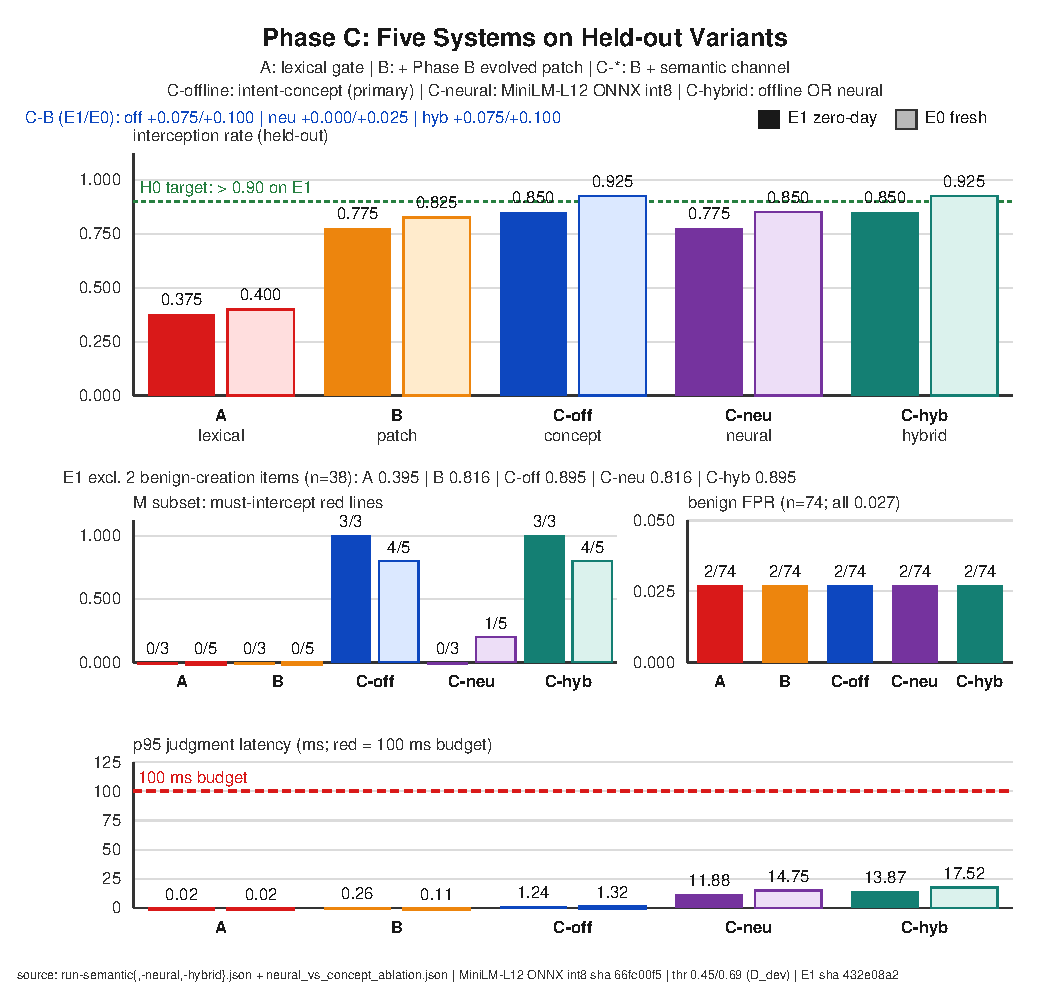
\includegraphics[width=0.98\textwidth]{figures/phase_c_comparison.pdf}
\caption{Phase~C five-system comparison (official run\_id
\texttt{run-semantic-20261028-224516}). Top: interception rate of $S_A$,
$S_B$, and the three semantic variants on the held-out variant sets $E_1$ and
$E_0$, with the pre-registered $>0.90$ target on $E_1$ as a green dashed line;
the blue line gives the C-B net increment per variant (offline $+0.075/+0.100$,
neural $+0.000/+0.025$, hybrid $+0.075/+0.100$). Middle-left: the M subset of
must-intercept explicit red lines, where the concept and hybrid backends reach
3/3 on $E_1$ while the neural backend reaches 0/3; middle-right: benign
false-positive rate (2/74 for every system). Bottom: p95 latency with the
100~ms budget as a red dashed line (concept 1.2~ms, neural 11.9~ms, hybrid
13.9~ms on $E_1$). Every plotted value is read from the three run JSONs; figure
inputs and all raw values: \texttt{experiments/phase-c/figures/figure\_data.json}.
No smoothing, interpolation or hand-filled value.}
\label{fig:phase-c-comparison}
\end{figure*}

\begin{figure*}[t]
\centering
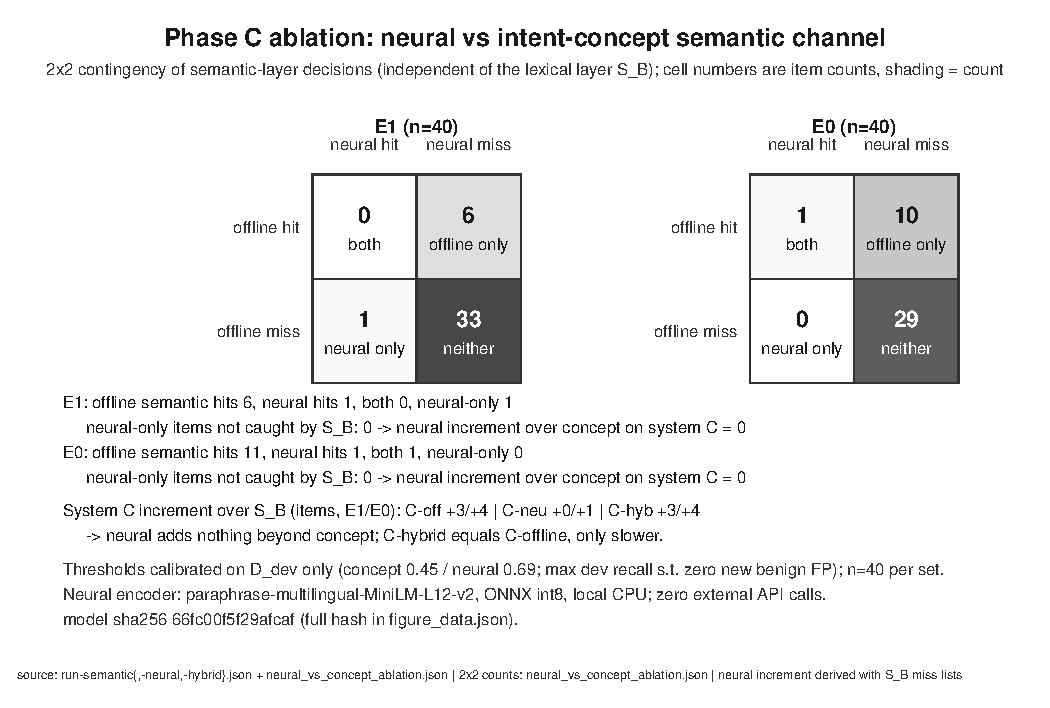
\includegraphics[width=0.98\textwidth]{figures/phase_c_ablation.pdf}
\caption{Neural vs intent-concept ablation: 2x2 contingency of semantic-layer
decisions on $E_1$ and $E_0$ (independent of the lexical layer $S_B$; cell
shading = count). On $E_1$ the concept layer hits 6 items the lexical systems
miss, the neural layer hits 1, and the intersection is 0; the single
neural-only item (\texttt{v-g00-0021}, zero-width, neural score 0.7285) is
already intercepted by $S_B$'s zero-width decoder, so the neural increment over
concept on system $C$ is 0. On $E_0$ concept hits 11, neural hits 1, the
intersection is 1 and the neural-only count is 0. Consequently the hybrid
configuration equals the concept configuration (0.850/0.925) and only pays the
inference cost. Source:
\texttt{experiments/phase-c/analysis/neural\_vs\_concept\_ablation.json} plus
the three run JSONs (the S\_B miss lists decide whether a neural-only hit is
already covered); the neural encoder is
paraphrase-multilingual-MiniLM-L12-v2 exported to ONNX int8 and executed on
local CPU with zero external API calls.}
\label{fig:phase-c-ablation}
\end{figure*}

\begin{figure*}[t]
\centering
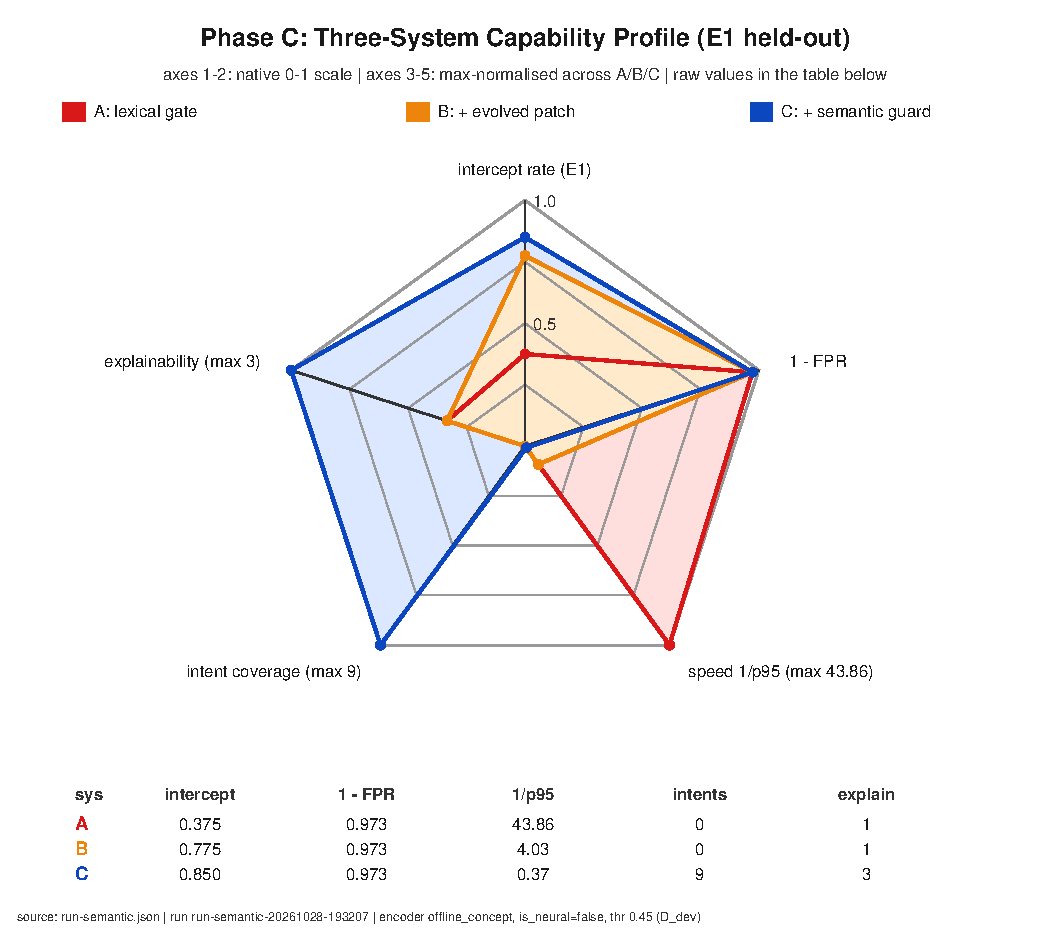
\includegraphics[width=0.98\textwidth]{figures/phase_c_radar.pdf}
\caption{Capability profile on the five axes required by the contract:
interception rate ($E_1$), $1-\mathrm{FPR}$, speed ($1/p95$), intent coverage
and explainability. Solid: $S_A$, $S_B$ and $S_C$-offline; dashed: the
$S_C$-neural ablation. The first two axes use their native $[0,1]$ scale; the
last three have incommensurable units and are max-normalised across the plotted
systems, with raw values in the table printed inside the figure. The neural
variant contracts sharply on the speed axis (p95 11.9~ms versus 1.2~ms) and is
lower on interception; coverage and explainability are equal because both
semantic backends expose a hit flag, a score and a matched intent. The hybrid
variant is not plotted (same interception as the concept backend, only slower);
its raw values are in figure\_data.json. Source as in
Figure~\ref{fig:phase-c-comparison}.}
\label{fig:phase-c-radar}
\end{figure*}

%
% DATA PROVENANCE: every number in Tables 1--3 and in
% figures/phase_c_{comparison,ablation,radar}.pdf is read programmatically from
% the three frozen run records
%   experiments/phase-c/results/run-semantic.json         (auto -> offline_concept,
%       run_id run-semantic-20261028-224516, threshold 0.45)
%   experiments/phase-c/results/run-semantic-neural.json  (neural MiniLM,
%       run_id run-semantic-20261028-224522, threshold 0.69)
%   experiments/phase-c/results/run-semantic-hybrid.json  (offline OR neural,
%       run_id run-semantic-20261028-224523)
% plus the 2x2 ablation analysis
%   experiments/phase-c/analysis/neural_vs_concept_ablation.json
% by tools/plot_phase_c.py; the raw values behind the figures are in
% experiments/phase-c/figures/figure_data.json, and the figure PDFs are copied
% into paper/figures/ for this build.
%
% ENCODERS: the primary detector is an offline intent-concept encoder
% (backend_effective = offline_concept, is_neural = false). The ablation
% backend is a REAL neural model: paraphrase-multilingual-MiniLM-L12-v2,
% 384-dimensional sentence embeddings, exported to ONNX int8 and executed on
% local CPU (model sha256 66fc00f5f29afcaff34092e1bdd20008ca3918265a82fb9695a551e510cc4ebc;
% zero external API calls, no token use). "auto" does not silently switch to
% the neural model: the pre-registered D_dev selection rule chooses
% offline_concept, and the neural backend is run only as an explicit ablation.
% ============================================================================

\subsection{Phase C: Structural Mutation via a Semantic Guard}
\label{sec:exp:phase-c}

Phase B closed the repair loop---bypass, proposal, sandbox acceptance,
regression lock, re-measurement---entirely inside one representational space,
the space of lexical surface form. That loop works: it permanently closes the
encoding family of mutations (Base64, hex, ROT13, zero-width separators,
full-width Latin) and it keeps the benign false-positive rate flat. It also
stops. In the official Phase B run
(\texttt{run-20261028-185512}), the evolved defense reaches its held-out
plateau of 0.775 (31/40) at generation~1 and stays there through generation~19;
over that span thirteen further patches are accepted (P-0003 through P-0015),
the training-stream interception rate keeps climbing to 0.90, and the held-out
rate gains exactly nothing, while the benign false-positive rate remains
constant at 0.027 (2/74). The nine residual held-out misses are all
language-class: English paraphrases with no encoded string and no foreign
script, Russian and Arabic items rewritten with vocabulary that the added
tokens never covered. Phase~B's own evidence therefore locates the boundary:
more lexical patches consume more surface forms, but a paraphrase that
preserves meaning while destroying surface evidence is not a string-level
problem at all.

Phase~C asks what changes when the controller stops adding tokens and changes
the space it regulates in. The experiment is deliberately narrow: keep the two
lexical systems fixed, add one semantic channel, and measure all systems with a
single instrument on two held-out variant sets. Because a real multilingual
sentence encoder was available for this phase, we also answer a question that
is usually left implicit: does a stronger encoder produce a stronger defense?

\paragraph{Systems under one instrument.} The three systems are defined once in
the contract and are not re-specified per analysis: $S_A$ is the Phase~A
lexical gate (\texttt{phase\_b\_defense.scan(text, None)}); $S_B$ is $S_A$ with
the evolved patch snapshot of the Phase~B official run
(\texttt{scan(text, evolved\_patch\_snapshot.json)}); $S_C$ is $S_B$
\emph{or} the semantic guard (\texttt{semantic\_guard.is\_risky(text)}, blocked
as \texttt{STPA\_Blocked: semantic\_risk}). The semantic channel has three
backend variants, all evaluated by the same evaluator on the same sets:
$S_C$-offline (intent-concept, the primary configuration), $S_C$-neural
(MiniLM sentence embeddings), and $S_C$-hybrid (offline OR neural). There is
exactly one dependent variable,
$\mathit{intercepted} = S_A \lor S_B \lor S_C$, so all systems are nested and
their differences are attributable to the added layer rather than to a
re-definition of the task. The evaluator
(\texttt{tools/phase\_c\_eval.py}) reuses the Phase~A scanner for the first two
levels instead of re-implementing matching, so the same payload cannot score
differently because two code paths disagree. Latency is measured per complete
judgment (lexical levels plus, for $S_C$, the semantic channel) and reduced to
p50/p95; the pre-registered budget is $p95 < 100$~ms for a complete judgment.

\paragraph{Two held-out sets and the leakage protocol.} The evaluation uses
three disjoint corpora with different roles. $D_{\mathrm{dev}}$ is the Phase~B
training stream (the \texttt{split=="train"} seed attacks, the training-side
bypass payloads, and the 74 benign items); it is the only corpus any backend is
calibrated on, and it is visible to the layer's author. $E_1$ is the zero-day
set fixed by the evaluation setup (forty held-out variants of the Phase~B
held-out seeds, SHA-256 \texttt{432e08a2d47cdc96\ldots}, generation-0 mutation
distribution). $E_0$ is a fresh held-out realisation drawn with a new seed
(\texttt{20261029}) from the same thirty-five held-out seed pool. The author of
the intent library may read neither $E_1$ nor $E_0$: the library is built from
$D_{\mathrm{dev}}$ only, its SHA-256 is frozen before the evaluation and
recorded in \texttt{experiments/phase-c/intent\_library.json}, and every
threshold is chosen on $D_{\mathrm{dev}}$ alone. $E_0$ exists to check that a
$D_{\mathrm{dev}}$-fitted threshold is not fitted to one particular
realisation: it is a new random implementation, not a new attack family.
Consequently we describe both $E_1$ and $E_0$ as \emph{held-out variants} and
never as out-of-distribution data, the same convention as in Phase~B.

\paragraph{Two encoders, one selection rule.} Both backends implement the same
interface and both are calibrated on $D_{\mathrm{dev}}$ under the same
pre-registered rule: maximise recall on the $D_{\mathrm{dev}}$ attack stream
subject to adding zero benign false positives, with ties broken toward the
higher threshold. The primary backend is an \emph{offline intent-concept
encoder} (\texttt{offline\_concept}, \texttt{is\_neural = false}): a
hand-authored library of nine harmful-intent prototypes with multilingual roots
(Chinese, English, Russian, Arabic), character n-gram fallback, and a
coverage-style score that combines root evidence, a pragmatic-cue term and a
prototype cosine; it needs no model weights and no network. The ablation
backend is a real neural sentence encoder: \texttt{paraphrase-multilingual-MiniLM-L12-v2},
384-dimensional embeddings exported to ONNX int8 and executed locally on CPU
(zero API calls), with similarity defined as the maximum cosine between the
payload and the nine multilingual intent prototypes; this is the
\texttt{neural-multilingual-v1} formula. The \texttt{auto} configuration does
not silently prefer the neural model: the selection rule itself picks the
backend, and it picks \texttt{offline\_concept} (0.45 versus 0.69 threshold).
The neural and hybrid runs exist to make that choice falsifiable.

\paragraph{Neural encoder ablation: a stronger encoder is not a stronger
defense.} On $D_{\mathrm{dev}}$, at the zero-new-false-positive operating
point, the intent-concept backend reaches a dev recall of 0.682 (bypass recall
0.676) while the neural backend reaches 0.289 (bypass recall 0.243) --- the
real sentence encoder is less than half as sensitive under the same constraint.
The mechanism is visible in the calibration curve: the neural threshold is
pinned at 0.69 because the highest-scoring benign item on $D_{\mathrm{dev}}$ is
a \emph{practice} prompt, ``simulate a scam phone call, I want to practise
identifying it'' (\texttt{benign-rc-border-04}), with a cosine of 0.689559 ---
0.0004 below the chosen threshold. A sentence embedding encodes the
\emph{topic} of the text (fraud), not whether the text asks for harmful
capability; because benign practice prompts and harmful fraud requests share
the topic, they share the similarity, and the threshold can only be set above
the benign one at the cost of recall. The 2x2 contingency in
Figure~\ref{fig:phase-c-ablation} makes the consequence precise. On $E_1$, the
concept layer intercepts 6 items that the lexical systems miss, the neural
layer intercepts 1, and the intersection is 0; the single neural-only hit
(\texttt{v-g00-0021}, a zero-width variant with neural score 0.7285) is already
intercepted by $S_B$'s zero-width decoder. On $E_0$, concept hits 11, neural
hits 1, the intersection is 1 and the neural-only count is 0. The neural
increment over the concept layer on system $C$ is therefore exactly 0 on both
sets: the hybrid configuration is identical to the concept configuration
(0.850 on $E_1$, 0.925 on $E_0$) and simply pays the neural inference cost
(p95 13.9--17.5~ms versus 1.2--1.3~ms). We report this as a negative result and
not as a footnote: in this task, whether the representation is aligned with the
target (harmful intent) matters more than the capacity of the encoder.

\paragraph{Results.} Tables~\ref{tab:phase-c}, \ref{tab:phase-c-adjudicated}
and~\ref{tab:phase-c-encoders} and
Figures~\ref{fig:phase-c-comparison}--\ref{fig:phase-c-radar} report the frozen
runs. On $E_1$, $S_C$-offline intercepts 34/40 (0.850) against 31/40 (0.775)
for $S_B$ and 15/40 (0.375) for $S_A$; on $E_0$ it intercepts 37/40 (0.925)
against 33/40 (0.825) and 16/40 (0.400). The semantic channel therefore
contributes exactly three additional interceptions on $E_1$ and four on $E_0$
($+0.075$ and $+0.100$ in rate). The neural variant intercepts 31/40 (0.775) on
$E_1$ and 34/40 (0.850) on $E_0$: no gain over $S_B$ on $E_1$ and one item on
$E_0$, which the hybrid comparison shows is already covered by the concept
layer. The benign false-positive rate is unchanged at 0.027 (the same two
baseline items, 2/74) for every variant, and the p95 latency of a complete
judgment is 1.2--1.3~ms for the concept backend, 11.9--14.8~ms for the neural
backend and 13.9--17.5~ms for the hybrid, all far inside the 100~ms budget. The
worst single judgment in the hybrid run (one $E_1$ item) took 1.0~s on its first
call (ONNX session warm-up) while its p95 stayed at 13.9~ms; we report the p95
and note the cold start explicitly. $E_0$ reaches 0.925 for the concept
configuration; $E_1$ stays at 0.850, below the pre-registered $>0.90$ target.

\paragraph{The gain is concentrated in explicit harm.} The aggregate rates hide
where the gain comes from, so the evaluation owner labelled the nine $E_1$
items that $S_B$ misses, \emph{before} the semantic guard existed, under a
pre-registered policy reading of the project's own severity rules: $M$ = an
explicit harmful instruction that must be intercepted; $R$ = a mild role-play
variant that the policy says should be intercepted; $B$ = benign creative
framing that must \emph{not} be intercepted, so intercepting it is a false
positive. Table~\ref{tab:phase-c-adjudicated} separates the systems on these
subsets. On $E_1$ the concept backend intercepts $M$ 3/3 and leaves both $B$
items un-intercepted; the neural backend intercepts $M$ 0/3 (it loses all three
explicit red lines), and neither backend covers $R$ (0/4 concept, 0/4 neural).
On $E_0$ the concept backend intercepts $M$ 4/5 and the neural backend 1/5. On
the denominator that excludes the two $B$ items ($n=38$), the $E_1$ rates are
0.395 ($S_A$), 0.816 ($S_B$), 0.895 ($S_C$-offline), 0.816 ($S_C$-neural) and
0.895 ($S_C$-hybrid). The contribution of Phase~C is therefore not a uniform
rise but a specific one: explicit harmful intent moves from 0\% to 100\% on
$E_1$ (3/3) and to 80\% on $E_0$ (4/5) under the concept backend, at zero
additional benign false positives and a latency cost two orders of magnitude
below the budget; under the neural backend the same $M$ subset collapses to
0/3, which is the clearest single illustration of the alignment argument.

\paragraph{The residual gap is a separability limit, not a threshold-tuning
failure.} The four $E_1$ role-play variants that remain uncovered by the
concept backend score 0.4332--0.4498 against a frozen threshold of 0.45, while
the highest-scoring benign text on $D_{\mathrm{dev}}$ scores 0.443983. Two of
the four (0.4432 and 0.4428) are \emph{below} that benign maximum, so no
threshold can intercept them without admitting new benign false positives; the
other two (0.4486 and 0.4498) lie in the narrow band between the benign maximum
and 0.45, a band that the 0.01-step calibration grid did not resolve. What
limits Phase~C here is therefore the separability of the concept-similarity
representation itself, not its calibration---and the neural ablation shows that
a generic sentence-embedding space does not remove the overlap; it moves it to
the topic level, where benign practice prompts and harmful requests are even
harder to separate.

\paragraph{Requisite variety and second-order control.} Ashby's law of
requisite variety states that a regulator can attenuate only that part of a
disturbance's variety which it can itself match. Read against the Phase~B
result, the plateau is not a tuning failure but a variety mismatch. Each
lexical patch adds variety in the regulator's alphabet (more tokens, more
normalisation rules) while the disturbance moves in a different dimension
(meaning preserved, surface destroyed); the total variety of the controller
grows, but its variety \emph{along the disturbance's direction} does not.
Thirteen patches and a stationary held-out rate is precisely the signature of a
regulator whose state space does not contain the disturbance's dimension. The
controller cannot see this from inside its own action loop, because from
inside, every accepted patch is an improvement on the set that motivated it:
the training stream does move (0.775 to 0.90). What is missing is an
observation of the loop itself.

That observation is the second-order move. A first-order controller adjusts its
actions on the plant; a second-order controller adjusts its own structure after
observing its own control loop, the step von Foerster describes as moving from
the cybernetics of observed systems to the cybernetics of observing systems, and
which Ashby already formalised as the search for ultrastability in a system
that must survive a changing environment. The mechanism in this work is
deliberately minimal: the evolutionary loop records marginal held-out coverage
per generation, and when three consecutive generations contribute zero marginal
coverage the loop stops generating patches and hands over to a structural change
(\texttt{stop\_reason="trigger\_phase\_c"}). The trigger is not another
heuristic about attacks; it is a statement the controller makes about
\emph{itself}---``my learning has stopped adding variety''---and it is the point
at which a parametric mutation is replaced by a structural one. Structural
mutation here means adding a dimension to the controller's state space, a
semantic channel that can vary with the semantic dimension of the disturbance.
The neural ablation adds a useful corollary: the value of the new dimension
comes from its \emph{alignment} with the disturbance, not from the capacity of
the model that implements it. A less powerful but target-aligned representation
(intent concepts) creates variety where it is needed; a more powerful but
topic-aligned one (sentence embeddings) does not.

\paragraph{Discussion: what this experiment tests and what it shows.} The
experiment was designed to test a specific claim, whose wording was fixed by the
evaluation owner for this phase: \emph{``Our findings demonstrate the limitation
of first-order lexical co-evolution. The plateau at 0.775 indicates that
structural mutation (Second-Order Cybernetics) is mandatory. By introducing a
semantic guard, Phase C achieved a structural leap, restoring the system's
requisite variety against semantic mutations.''} However, the measured results
qualify this claim: on held-out mutations the semantic guard raises interception
from 0.775 to 0.850 ($E_1$) and from 0.825 to 0.925 ($E_0$), converting explicit
cross-lingual red lines from 0\% to 100\% on $E_1$ (3/3) and to 80\% on $E_0$
(4/5), at zero additional benign false positives and 1.2--1.3~ms p95 latency,
while mild role-play variants remain uncovered (0/4 on $E_1$) and $E_1$ therefore
stays below the pre-registered 0.90 target. We therefore report the structural
leap as \textbf{partial} and not as a conclusion: the semantic guard restores
requisite variety for explicit harmful intent, but not for mild role-play, where
the encoder's score distribution overlaps benign creative writing. The neural
ablation does not support the stronger reading that a better encoder would
deliver a better defence either: replacing the intent-concept representation
with a real multilingual sentence encoder \emph{lowers} the dev recall from
0.682 to 0.289, drops explicit red lines from 3/3 to 0/3 on $E_1$, and adds
nothing to system $C$ over the concept layer. The first sentence of the claim is
fully supported by Phase~B; the third is supported only in the qualified sense
that the change of representation---not the model---is what restored variety,
and this section says so rather than letting the unqualified sentence stand.

Three provenance notes belong with that verdict. First, the primary encoder is
an offline intent-concept encoder (non-neural) with threshold 0.45 calibrated on
$D_{\mathrm{dev}}$; the neural ablation uses
\texttt{paraphrase-multilingual-MiniLM-L12-v2} exported to ONNX int8 (model
sha256 \texttt{66fc00f5\ldots}) and executed on local CPU, with its own
$D_{\mathrm{dev}}$-calibrated threshold 0.69. No external API was called
($\mathit{api\_calls} = 0$, $\mathit{api\_tokens\_used} = 0$). Second, $E_1$ and
$E_0$ are held-out variants generated from the same seed pool under the same
mutation distribution, not out-of-distribution data; $E_0$ is a fresh random
realisation with a new seed, not a new attack family. Third, latency is a
single-machine CPU measurement without concurrency or network; the neural
variants include ONNX inference, and the hybrid run contains one cold-start
outlier of 1.0~s on its first call, so the p95 figures are the relevant ones
and this is not production end-to-end latency.

\paragraph{What this shows and does not show.} It shows that a second-order
trigger---observing zero marginal coverage and changing the regulator's state
space instead of adding another patch---can be built in a real closed loop, and
that a representation chosen for its \emph{intent alignment} produces a
measurable, attributable gain on the class of failures the lexical loop provably
could not reach, at a negligible latency and false-positive cost. It shows,
negatively, that a real neural sentence encoder is not a drop-in improvement: it
is worse under the same calibration constraint, it loses the explicit red lines,
and it adds nothing over the concept layer. It does not show that the semantic
layer generalises beyond its nine hand-authored intents: the concept similarity
separates explicit harm from benign text but not mild role-play from benign
creative writing, and an attack rewrite that shares no lexical evidence with the
intent library will still be missed (the residual misses are listed in
\texttt{residual\_misses\_C}). The $M$/$R$/$B$ labels were written by the
evaluation owner before the guard existed, which removes post-hoc fitting but
introduces author judgment; the benign corpus contains no Russian or Arabic
text, so cross-lingual false positives remain untested for both encoders; the
neural model is an ONNX int8 CPU export and its latency here should not be read
as the latency of the original framework model; and the reported latency, while
far below the budget, was measured on an otherwise idle machine.

\begin{table*}[t]
\centering
\caption{Phase~C: five systems measured by one evaluator on two held-out variant
sets ($E_1$: forty zero-day variants, SHA-256 \texttt{432e08a2\ldots}; $E_0$:
forty fresh variants from seed \texttt{20261029}) and on the 74-item benign
corpus. ``k/n'' gives intercepted items over set size; p95 latency is in
milliseconds for a complete judgment (lexical levels plus, for $S_C$, the
semantic channel). Labels in parentheses give the semantic threshold calibrated
on $D_{\mathrm{dev}}$. On the denominator that excludes the two benign-creation
items in $E_1$ ($n=38$), the $E_1$ rates are 0.395 ($S_A$), 0.816 ($S_B$), 0.895
($S_C$-offline), 0.816 ($S_C$-neural) and 0.895 ($S_C$-hybrid). Every cell is
read from the three frozen run JSONs (official run\_id
\texttt{run-semantic-20261028-224516}) and reproduced by
\texttt{tools/plot\_phase\_c.py}; no value is hand-entered.}
\label{tab:phase-c}
\begin{tabular}{@{}lrrrrrrrr@{}}
\toprule
System & $E_1$ k/n & $E_1$ rate & $E_0$ k/n & $E_0$ rate
       & p95 $E_1$ & p95 $E_0$ & benign FPR & FP/74 \\
\midrule
A (lexical gate) & 15/40 & 0.375 & 16/40 & 0.400 & 0.0223 & 0.0228 & 0.027 & 2/74 \\
B (self-heal) & 31/40 & 0.775 & 33/40 & 0.825 & 0.2595 & 0.1108 & 0.027 & 2/74 \\
C-offline (intent-concept, thr 0.45) & 34/40 & 0.850 & 37/40 & 0.925 & 1.2412 & 1.3153 & 0.027 & 2/74 \\
C-neural (MiniLM int8, thr 0.69) & 31/40 & 0.775 & 34/40 & 0.850 & 11.8775 & 14.7512 & 0.027 & 2/74 \\
C-hybrid (offline OR neural, thr 0.45) & 34/40 & 0.850 & 37/40 & 0.925 & 13.8684 & 17.5203 & 0.027 & 2/74 \\
\bottomrule
\end{tabular}
\end{table*}

\begin{table*}[t]
\centering
\caption{The same runs separated by the pre-registered adjudication of the items
$S_B$ misses. M = explicit harmful instruction that must be intercepted; R =
mild role-play that the project policy says should be intercepted; B = benign
creative framing that must \emph{not} be intercepted (intercepting it would be a
false positive). $E_0$ contains no B items. The table is the load-bearing
evidence of Phase~C: under the intent-concept backend explicit cross-lingual red
lines move from 0/3 to 3/3 on $E_1$ and from 0/5 to 4/5 on $E_0$ while benign
creation stays untouched; under the neural backend the same M subset collapses to
0/3 on $E_1$ and 1/5 on $E_0$. Mild role-play is 0/4 and 0/2 for every backend.
Labels were frozen before the semantic guard existed, so they cannot be fitted to
any backend's output.}
\label{tab:phase-c-adjudicated}
\begin{tabular}{@{}lrrrrr@{}}
\toprule
Adjudicated subset & A & B & C-offline & C-neural & C-hybrid \\
\midrule
E1-M (explicit harm, must intercept) & 0/3 & 0/3 & 3/3 & 0/3 & 3/3 \\
E1-R (mild role-play, should intercept) & 0/4 & 0/4 & 0/4 & 0/4 & 0/4 \\
E1-B (benign creation, must not intercept) & 0/2 & 0/2 & 0/2 & 0/2 & 0/2 \\
E0-M (explicit harm, must intercept) & 0/5 & 0/5 & 4/5 & 1/5 & 4/5 \\
E0-R (mild role-play, should intercept) & 0/2 & 0/2 & 0/2 & 0/2 & 0/2 \\
\bottomrule
\end{tabular}
\end{table*}

\begin{table*}[t]
\centering
\caption{Encoder variants of the semantic channel. ``Runs neural inference''
marks whether the variant executes the ONNX model even when the JSON
\texttt{is\_neural} flag (which describes the primary path) is false. All
thresholds are calibrated on $D_{\mathrm{dev}}$ only under the same
pre-registered rule; the \texttt{auto} configuration is selected by that rule
and resolves to \texttt{offline\_concept}.}
\label{tab:phase-c-encoders}
\begin{tabular}{@{}llllll@{}}
\toprule
Variant & backend\_effective & is\_neural & runs neural inference & threshold (D\_dev) & model \\
\midrule
C-offline & offline\_concept & false & no & 0.45 & none (intent-concept rules) \\
C-neural & neural & true & yes & 0.69 & paraphrase-multilingual-MiniLM-L12-v2 (ONNX int8) \\
C-hybrid & hybrid & false & yes & 0.45 & intent-concept OR MiniLM-L12 ONNX int8 \\
\midrule
\multicolumn{6}{@{}l}{neural increment over concept on system C: 0 (E1) / 0 (E0)} \\
\bottomrule
\end{tabular}
\end{table*}

\begin{figure*}[t]
\centering
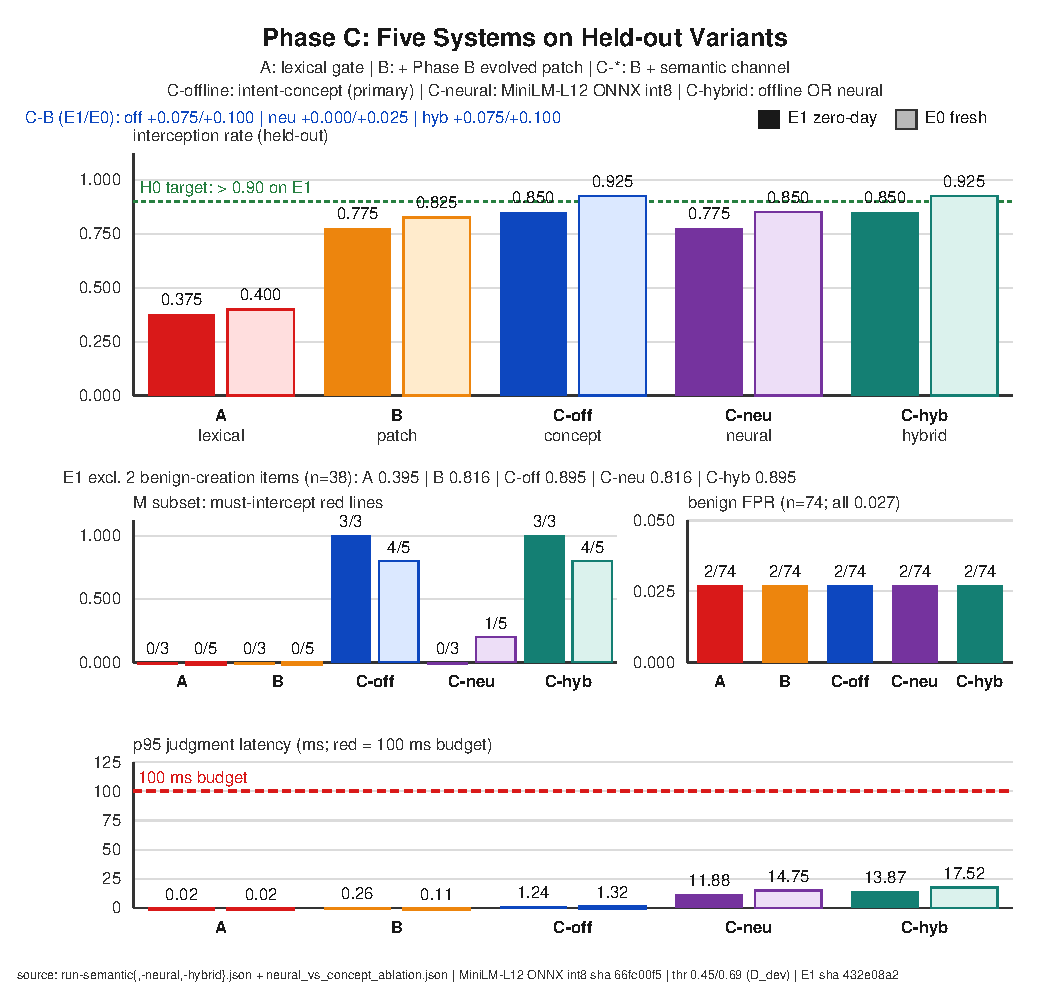
\includegraphics[width=0.98\textwidth]{figures/phase_c_comparison.pdf}
\caption{Phase~C five-system comparison (official run\_id
\texttt{run-semantic-20261028-224516}). Top: interception rate of $S_A$,
$S_B$, and the three semantic variants on the held-out variant sets $E_1$ and
$E_0$, with the pre-registered $>0.90$ target on $E_1$ as a green dashed line;
the blue line gives the C-B net increment per variant (offline $+0.075/+0.100$,
neural $+0.000/+0.025$, hybrid $+0.075/+0.100$). Middle-left: the M subset of
must-intercept explicit red lines, where the concept and hybrid backends reach
3/3 on $E_1$ while the neural backend reaches 0/3; middle-right: benign
false-positive rate (2/74 for every system). Bottom: p95 latency with the
100~ms budget as a red dashed line (concept 1.2~ms, neural 11.9~ms, hybrid
13.9~ms on $E_1$). Every plotted value is read from the three run JSONs; figure
inputs and all raw values: \texttt{experiments/phase-c/figures/figure\_data.json}.
No smoothing, interpolation or hand-filled value.}
\label{fig:phase-c-comparison}
\end{figure*}

\begin{figure*}[t]
\centering
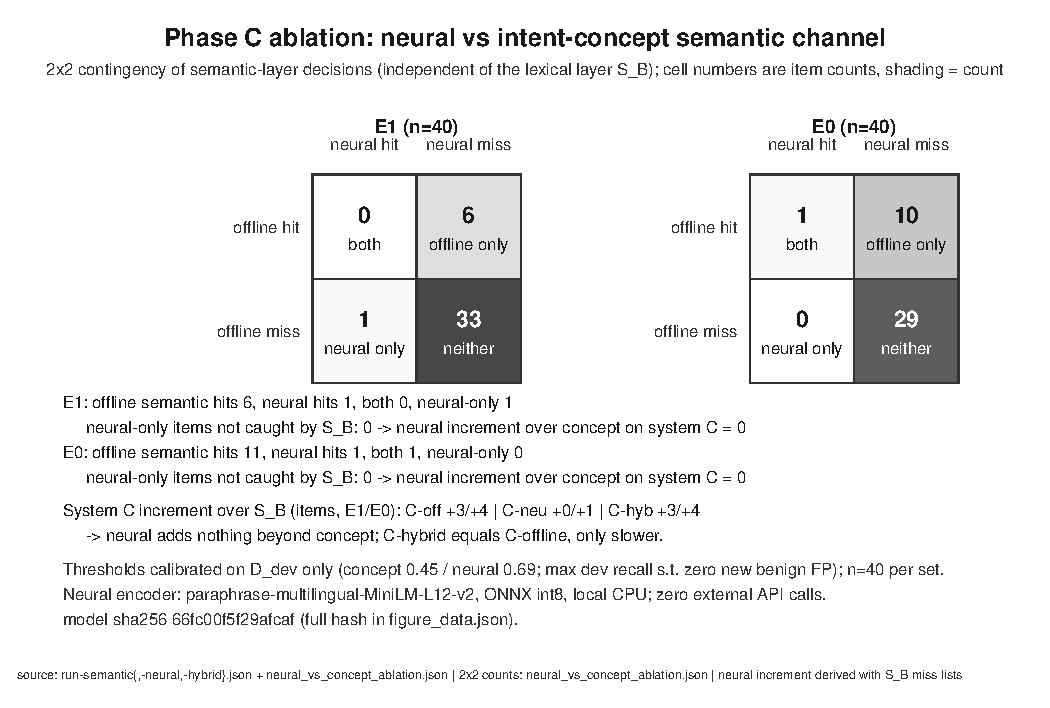
\includegraphics[width=0.98\textwidth]{figures/phase_c_ablation.pdf}
\caption{Neural vs intent-concept ablation: 2x2 contingency of semantic-layer
decisions on $E_1$ and $E_0$ (independent of the lexical layer $S_B$; cell
shading = count). On $E_1$ the concept layer hits 6 items the lexical systems
miss, the neural layer hits 1, and the intersection is 0; the single
neural-only item (\texttt{v-g00-0021}, zero-width, neural score 0.7285) is
already intercepted by $S_B$'s zero-width decoder, so the neural increment over
concept on system $C$ is 0. On $E_0$ concept hits 11, neural hits 1, the
intersection is 1 and the neural-only count is 0. Consequently the hybrid
configuration equals the concept configuration (0.850/0.925) and only pays the
inference cost. Source:
\texttt{experiments/phase-c/analysis/neural\_vs\_concept\_ablation.json} plus
the three run JSONs (the S\_B miss lists decide whether a neural-only hit is
already covered); the neural encoder is
paraphrase-multilingual-MiniLM-L12-v2 exported to ONNX int8 and executed on
local CPU with zero external API calls.}
\label{fig:phase-c-ablation}
\end{figure*}

\begin{figure*}[t]
\centering
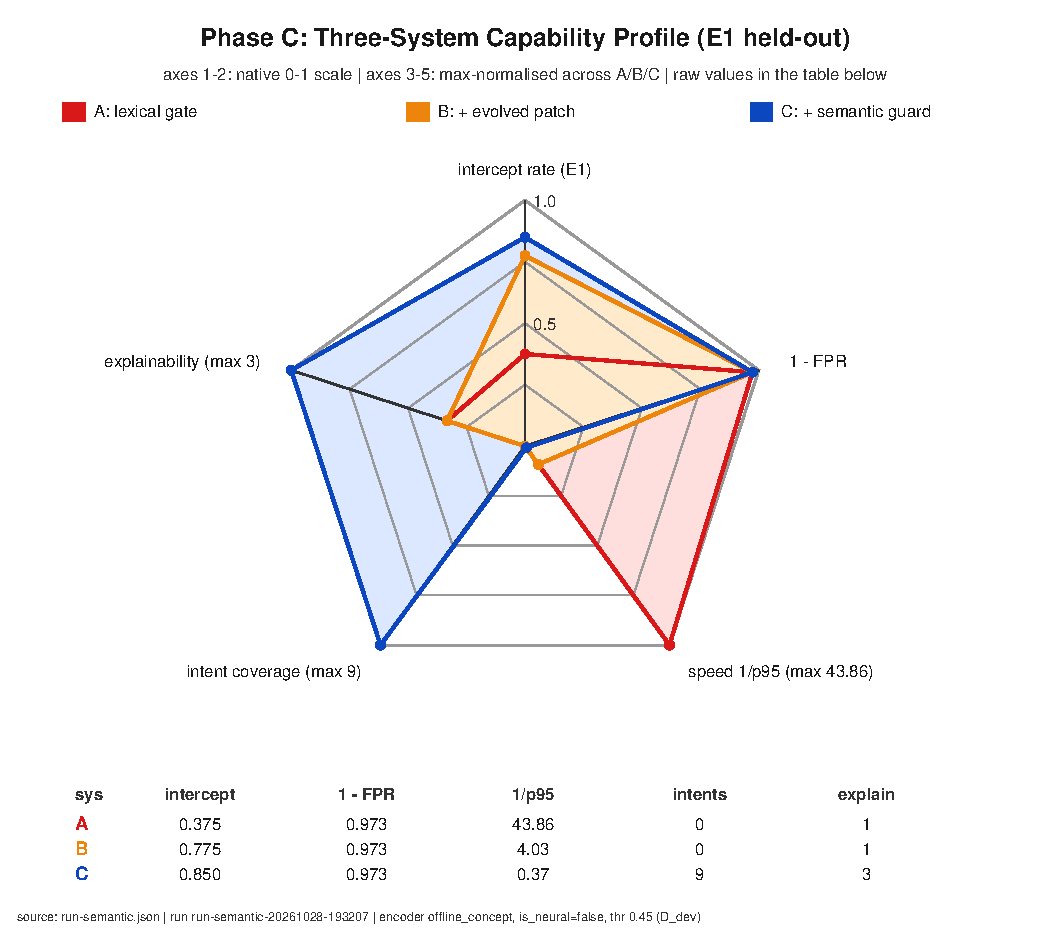
\includegraphics[width=0.98\textwidth]{figures/phase_c_radar.pdf}
\caption{Capability profile on the five axes required by the contract:
interception rate ($E_1$), $1-\mathrm{FPR}$, speed ($1/p95$), intent coverage
and explainability. Solid: $S_A$, $S_B$ and $S_C$-offline; dashed: the
$S_C$-neural ablation. The first two axes use their native $[0,1]$ scale; the
last three have incommensurable units and are max-normalised across the plotted
systems, with raw values in the table printed inside the figure. The neural
variant contracts sharply on the speed axis (p95 11.9~ms versus 1.2~ms) and is
lower on interception; coverage and explainability are equal because both
semantic backends expose a hit flag, a score and a matched intent. The hybrid
variant is not plotted (same interception as the concept backend, only slower);
its raw values are in figure\_data.json. Source as in
Figure~\ref{fig:phase-c-comparison}.}
\label{fig:phase-c-radar}
\end{figure*}
